% Options for packages loaded elsewhere
\PassOptionsToPackage{unicode}{hyperref}
\PassOptionsToPackage{hyphens}{url}
%
\documentclass[
]{book}
\usepackage{lmodern}
\usepackage{amssymb,amsmath}
\usepackage{ifxetex,ifluatex}
\ifnum 0\ifxetex 1\fi\ifluatex 1\fi=0 % if pdftex
  \usepackage[T1]{fontenc}
  \usepackage[utf8]{inputenc}
  \usepackage{textcomp} % provide euro and other symbols
\else % if luatex or xetex
  \usepackage{unicode-math}
  \defaultfontfeatures{Scale=MatchLowercase}
  \defaultfontfeatures[\rmfamily]{Ligatures=TeX,Scale=1}
\fi
% Use upquote if available, for straight quotes in verbatim environments
\IfFileExists{upquote.sty}{\usepackage{upquote}}{}
\IfFileExists{microtype.sty}{% use microtype if available
  \usepackage[]{microtype}
  \UseMicrotypeSet[protrusion]{basicmath} % disable protrusion for tt fonts
}{}
\makeatletter
\@ifundefined{KOMAClassName}{% if non-KOMA class
  \IfFileExists{parskip.sty}{%
    \usepackage{parskip}
  }{% else
    \setlength{\parindent}{0pt}
    \setlength{\parskip}{6pt plus 2pt minus 1pt}}
}{% if KOMA class
  \KOMAoptions{parskip=half}}
\makeatother
\usepackage{xcolor}
\IfFileExists{xurl.sty}{\usepackage{xurl}}{} % add URL line breaks if available
\IfFileExists{bookmark.sty}{\usepackage{bookmark}}{\usepackage{hyperref}}
\hypersetup{
  pdftitle={R'da Ekonometri Uygulamaları},
  pdfauthor={Ahmet Akgül (rpydaneogrendim)},
  hidelinks,
  pdfcreator={LaTeX via pandoc}}
\urlstyle{same} % disable monospaced font for URLs
\usepackage{color}
\usepackage{fancyvrb}
\newcommand{\VerbBar}{|}
\newcommand{\VERB}{\Verb[commandchars=\\\{\}]}
\DefineVerbatimEnvironment{Highlighting}{Verbatim}{commandchars=\\\{\}}
% Add ',fontsize=\small' for more characters per line
\usepackage{framed}
\definecolor{shadecolor}{RGB}{248,248,248}
\newenvironment{Shaded}{\begin{snugshade}}{\end{snugshade}}
\newcommand{\AlertTok}[1]{\textcolor[rgb]{0.94,0.16,0.16}{#1}}
\newcommand{\AnnotationTok}[1]{\textcolor[rgb]{0.56,0.35,0.01}{\textbf{\textit{#1}}}}
\newcommand{\AttributeTok}[1]{\textcolor[rgb]{0.77,0.63,0.00}{#1}}
\newcommand{\BaseNTok}[1]{\textcolor[rgb]{0.00,0.00,0.81}{#1}}
\newcommand{\BuiltInTok}[1]{#1}
\newcommand{\CharTok}[1]{\textcolor[rgb]{0.31,0.60,0.02}{#1}}
\newcommand{\CommentTok}[1]{\textcolor[rgb]{0.56,0.35,0.01}{\textit{#1}}}
\newcommand{\CommentVarTok}[1]{\textcolor[rgb]{0.56,0.35,0.01}{\textbf{\textit{#1}}}}
\newcommand{\ConstantTok}[1]{\textcolor[rgb]{0.00,0.00,0.00}{#1}}
\newcommand{\ControlFlowTok}[1]{\textcolor[rgb]{0.13,0.29,0.53}{\textbf{#1}}}
\newcommand{\DataTypeTok}[1]{\textcolor[rgb]{0.13,0.29,0.53}{#1}}
\newcommand{\DecValTok}[1]{\textcolor[rgb]{0.00,0.00,0.81}{#1}}
\newcommand{\DocumentationTok}[1]{\textcolor[rgb]{0.56,0.35,0.01}{\textbf{\textit{#1}}}}
\newcommand{\ErrorTok}[1]{\textcolor[rgb]{0.64,0.00,0.00}{\textbf{#1}}}
\newcommand{\ExtensionTok}[1]{#1}
\newcommand{\FloatTok}[1]{\textcolor[rgb]{0.00,0.00,0.81}{#1}}
\newcommand{\FunctionTok}[1]{\textcolor[rgb]{0.00,0.00,0.00}{#1}}
\newcommand{\ImportTok}[1]{#1}
\newcommand{\InformationTok}[1]{\textcolor[rgb]{0.56,0.35,0.01}{\textbf{\textit{#1}}}}
\newcommand{\KeywordTok}[1]{\textcolor[rgb]{0.13,0.29,0.53}{\textbf{#1}}}
\newcommand{\NormalTok}[1]{#1}
\newcommand{\OperatorTok}[1]{\textcolor[rgb]{0.81,0.36,0.00}{\textbf{#1}}}
\newcommand{\OtherTok}[1]{\textcolor[rgb]{0.56,0.35,0.01}{#1}}
\newcommand{\PreprocessorTok}[1]{\textcolor[rgb]{0.56,0.35,0.01}{\textit{#1}}}
\newcommand{\RegionMarkerTok}[1]{#1}
\newcommand{\SpecialCharTok}[1]{\textcolor[rgb]{0.00,0.00,0.00}{#1}}
\newcommand{\SpecialStringTok}[1]{\textcolor[rgb]{0.31,0.60,0.02}{#1}}
\newcommand{\StringTok}[1]{\textcolor[rgb]{0.31,0.60,0.02}{#1}}
\newcommand{\VariableTok}[1]{\textcolor[rgb]{0.00,0.00,0.00}{#1}}
\newcommand{\VerbatimStringTok}[1]{\textcolor[rgb]{0.31,0.60,0.02}{#1}}
\newcommand{\WarningTok}[1]{\textcolor[rgb]{0.56,0.35,0.01}{\textbf{\textit{#1}}}}
\usepackage{longtable,booktabs}
% Correct order of tables after \paragraph or \subparagraph
\usepackage{etoolbox}
\makeatletter
\patchcmd\longtable{\par}{\if@noskipsec\mbox{}\fi\par}{}{}
\makeatother
% Allow footnotes in longtable head/foot
\IfFileExists{footnotehyper.sty}{\usepackage{footnotehyper}}{\usepackage{footnote}}
\makesavenoteenv{longtable}
\usepackage{graphicx,grffile}
\makeatletter
\def\maxwidth{\ifdim\Gin@nat@width>\linewidth\linewidth\else\Gin@nat@width\fi}
\def\maxheight{\ifdim\Gin@nat@height>\textheight\textheight\else\Gin@nat@height\fi}
\makeatother
% Scale images if necessary, so that they will not overflow the page
% margins by default, and it is still possible to overwrite the defaults
% using explicit options in \includegraphics[width, height, ...]{}
\setkeys{Gin}{width=\maxwidth,height=\maxheight,keepaspectratio}
% Set default figure placement to htbp
\makeatletter
\def\fps@figure{htbp}
\makeatother
\setlength{\emergencystretch}{3em} % prevent overfull lines
\providecommand{\tightlist}{%
  \setlength{\itemsep}{0pt}\setlength{\parskip}{0pt}}
\setcounter{secnumdepth}{5}
\usepackage{booktabs}
\usepackage[]{natbib}
\bibliographystyle{apalike}

\title{R'da Ekonometri Uygulamaları}
\author{Ahmet Akgül (rpydaneogrendim)}
\date{2020-05-16}

\begin{document}
\maketitle

{
\setcounter{tocdepth}{1}
\tableofcontents
}
\hypertarget{nelere-ihtiyacux131nux131z-olacak}{%
\chapter{Nelere İhtiyacınız Olacak?}\label{nelere-ihtiyacux131nux131z-olacak}}

Öncelikle R ve tavsiye olarak RStudio IDE'sini indirmenizi ve bu programlama dili hakkında bir miktar bilgi sahibi olmanızı tavsiye ederim. Çünkü bu kitapta R hakkında herhangi bir konu anlatımı olmayacaktır.

Ekonometri konularını akademik bir anlatımdan uzak tutmaya çalıştım fakat bu ezberci bir sistem ile öğreneceğiniz anlamına gelmeyecek. Her konu hakkında temel bir bilginiz olacak ve mutlaka en az bir uygulama yapmış olacaksınız.

Öğrenmek dinamik bir süreçtir. Temel bilgileri alır ve yaşamınız boyunca üzerine katarak ilerlemeye çalışırsınız. Bu kitap temel bir bilgi sahibi olmanızı amaçlamaktadır. Sonrası okuyucunun kendine kattıkları olacaktır.

\begin{quote}
\emph{İlim ve fennin yaşadığımız her dakikadaki safhalarının gelişmesini kavramak ve izlemek şarttır.} -Mustafa Kemal ATATÜRK
\end{quote}

\hypertarget{kullanux131lan-kuxfctuxfcphaneler}{%
\section{Kullanılan Kütüphaneler}\label{kullanux131lan-kuxfctuxfcphaneler}}

Kitap boyunca kullanacağımız kütüphaneler aşağıda verilmiştir:

\begin{Shaded}
\begin{Highlighting}[]
\KeywordTok{library}\NormalTok{(readxl)}
\KeywordTok{library}\NormalTok{(tidyverse)}
\KeywordTok{library}\NormalTok{(magrittr)}
\KeywordTok{library}\NormalTok{(HistData)}
\KeywordTok{library}\NormalTok{(moments)}
\KeywordTok{library}\NormalTok{(segmented)}
\KeywordTok{library}\NormalTok{(corrplot)}
\KeywordTok{library}\NormalTok{(psych)}
\KeywordTok{library}\NormalTok{(car)}
\KeywordTok{library}\NormalTok{(factoextra)}
\KeywordTok{library}\NormalTok{(FactoMineR)}
\KeywordTok{library}\NormalTok{(lmridge)}
\KeywordTok{library}\NormalTok{(AER)}
\KeywordTok{library}\NormalTok{(lmtest)}
\KeywordTok{library}\NormalTok{(estimatr)}
\KeywordTok{library}\NormalTok{(sandwich)}
\KeywordTok{library}\NormalTok{(nnet)}
\KeywordTok{library}\NormalTok{(mlogit)}
\KeywordTok{library}\NormalTok{(stargazer)}
\KeywordTok{library}\NormalTok{(Epi)}
\KeywordTok{library}\NormalTok{(MASS)}
\KeywordTok{library}\NormalTok{(VGAM)}
\KeywordTok{library}\NormalTok{(truncreg)}
\KeywordTok{library}\NormalTok{(ARDL)}
\KeywordTok{library}\NormalTok{(quantreg)}
\end{Highlighting}
\end{Shaded}

\hypertarget{kullanux131lan-veri-setleri}{%
\section{Kullanılan Veri Setleri}\label{kullanux131lan-veri-setleri}}

Kitap boyunca kullanılan veri setleri Github'da verilmiştir. Öncelikli olarak bu dosyayı indirmenizi tavsiye ederim.

\begin{itemize}
\item
  \href{https://github.com/rpydaneogrendim/rEkonometri}{Buraya tıklayın.}
\item
  \emph{Clone or download} bölümünden \emph{Download ZIP} seçeneği ile dosyaları indirebilirsiniz. Hedef dosya: \textbf{data}
\end{itemize}

\hypertarget{veri-ve-model-uxe7eux15fitleri}{%
\chapter{Veri ve Model Çeşitleri}\label{veri-ve-model-uxe7eux15fitleri}}

\hypertarget{veri-uxe7eux15fitleri}{%
\section{Veri Çeşitleri}\label{veri-uxe7eux15fitleri}}

\textbf{Zaman Serisi:} Bir değişkenin farklı zamanlarda aldığı değerler kümesine zaman serisi diyoruz. Günlük \$/TL kuru, haftalık para arzı, aylık enflasyon, üç aylık GSYH gibi çeşitli frekanslarda örnekler çoğaltılabilir. \textbf{Yatay-Kesit:} Bir veya daha fazla değişken için aynı zaman noktasında derlenen verilere yatay-kesit diyoruz. Nüfus sayımı, kamuoyu yoklamaları, illere göre araç sayıları gibi örnekler verilebilir. \textbf{Panel:} Hem zaman serisi hem de yatay-kesit verilerini bir araya getiren bu türe de panel diyoruz. Bankaların 20 yıllık döneme ait sermaye yeterlilik rasyoları, illerin bir ürüne ait 10 yıllık üretim değerleri gibi örnekler verilebilir.

\hypertarget{model-uxe7eux15fitleri}{%
\section{Model Çeşitleri}\label{model-uxe7eux15fitleri}}

Bu kitapta \textbf{regresyon} modellerini göreceğiz. Regresyon modelleri dışında kalan \textbf{zaman serisi modelleri}, \textbf{eşanlı denklem sistemleri} ve \textbf{panel veri} modelleri bu kitabın kapsamında değildir. Gelecek projelerde anlatılması planlanmaktadır.

\hypertarget{doux11frusal-regresyon-modeli}{%
\chapter{Doğrusal Regresyon Modeli}\label{doux11frusal-regresyon-modeli}}

İlk konunun çok önemli olduğunu düşünüyorum. Bu konuyu anlatabilen hoca da anlayan öğrenci de çok şey başarmış demektir. Greene, \emph{ekonometricinin alet çantasındaki en kullanışlı tek araç doğrusal regresyon modelidir} der. Gerekirse saatlerinizi yetmezse günlerinizi verin ama bu konuyu anlamadan asla diğer konulara geçmeyin.

Genel olarak doğrusal regresyon modelini şöyle yazarız:

\(Y_i = \beta_1 + \beta_2X_{2i} + \beta_3X_{3i} + ... + \beta_kX_{ki} + \epsilon_i\)

Y, bağımlı ya da açıklanan; X'ler bağımsız ya da açıklayıcı değişkenlerdir. \(\epsilon\), rassal ya da stokastik hata terimidir.

Yukarıda yazdığımız eşitliğe anakütle modeli denir. Anakütle kavramı kişiler, firmalar, şehirler gibi geneli temsil eder.

Eşitlikteki \(\beta_1\) kesme terimidir. \(\beta_2\) ile \(\beta_k\) arası ise eğim parametreleridir. Genel olarak \(\beta\), gerçek değerini bilmediğimiz ve istatistiki yöntemlerle tahmin etmeye çalıştığımız parametre kavramının sembolik ifadesidir.

\(\epsilon\), rassal ya da stokastik hata terimidir ve çeşitli nedenlerden dolayı modelde bulunamayan değişkenleri temsil eder. Stokastik sözcüğü hedef ya da hedefin göbeği anlamına gelir. Kennedy, stokastik ve hata terimini şu örnekle açıklar: \emph{Stokastik bir ilişki, okun nadiren hedefi tam on ikiden vurması gibi, bağımlı değişken değerinin tam olarak öngörülmesi anlamında, her zaman hedefi vuramaz. Hata terimi açıkça bu hedeften sapmaların ya da hataların büyüklüklerini belirlemek amacı ile kullanılır.} Hata terimi gibi bir de kalıntı elde edeceğiz. Bu, aynı anlama gelmekle beraber örneklem söz konusu olduğu zaman kullanılan bir ifadedir. Kennedy, hata terimi için \emph{ekonometristlerin kullandığı tahmin yöntemlerinin başarısı büyük bir oranda hata teriminin yapısına bağlıdır} der.

Öncelikli amacımız, X bağımsız değişkenlerinin değerlerindeki değişmeye Y'nin verdiği \emph{ortalama} tepkiyi bulmaktır. Başka bir ifade ile diğer değişkenleri sabit tutarak bir tane bağımsız değişkenin Y bağımlı değişkeni üzerindeki 1 birimlik etkisini her biri için ölçeriz.

Doğrusal dediğimiz zaman buradaki doğrusallığın değişkenlerden (X'ler) değil; parametrelerden (\(\beta'lar\)) geldiğini bilmemiz gerekiyor. Bağımlı ve bağımsız değişken(ler) logaritmik, tersi veya kuvveti alınmış şekilde olabilir. Bu, doğrusallık kavramını etkilemez. Asıl önemli olan \(\beta\) parametrelerinin kuvvetinin alınmaması, diğer parametrelere bölünmemesi veya dönüştürülmemesidir.

Bu kısa bilgilerden sonra uygulamaya geçebiliriz.

ABD Nüfus İdaresi'nin 1289 (anakütleden alınmış örneklem) kişi ile yaptığı araştırmasından elde edilen veri setini kullanacağız.

\begin{Shaded}
\begin{Highlighting}[]
\KeywordTok{library}\NormalTok{(readxl);}\KeywordTok{library}\NormalTok{(tidyverse);}\KeywordTok{library}\NormalTok{(magrittr)}

\KeywordTok{setwd}\NormalTok{(}\StringTok{"C:/Users/datanerd/Desktop/Github/rEkonometri/data"}\NormalTok{) }\CommentTok{#Dosyaları kaydettiğiniz yeri ayarlamalısınız.}
\NormalTok{df <-}\StringTok{ }\KeywordTok{read_excel}\NormalTok{(}\StringTok{"Table1_1.xls"}\NormalTok{)}
\end{Highlighting}
\end{Shaded}

\begin{Shaded}
\begin{Highlighting}[]
\NormalTok{df }\OperatorTok\StringTok{ }
\StringTok{  }\NormalTok{dplyr}\OperatorTok{::}\KeywordTok{select}\NormalTok{(wage, female, nonwhite, union, education, exper) }\CommentTok{#Kullanacağımız değişkenler.}

\KeywordTok{str}\NormalTok{(df)}
\end{Highlighting}
\end{Shaded}

\begin{verbatim}
## tibble [1,289 x 6] (S3: tbl_df/tbl/data.frame)
##  $ wage     : num [1:1289] 11.6 5 12 7 21.1 ...
##  $ female   : num [1:1289] 1 0 0 0 1 1 1 1 0 1 ...
##  $ nonwhite : num [1:1289] 0 0 0 1 1 0 0 1 0 0 ...
##  $ union    : num [1:1289] 0 0 0 1 0 0 0 0 0 0 ...
##  $ education: num [1:1289] 12 9 16 14 16 12 12 12 18 18 ...
##  $ exper    : num [1:1289] 20 9 15 38 19 4 14 32 7 5 ...
\end{verbatim}

Bağımlı değişken:

\begin{itemize}
\tightlist
\item
  \textbf{wage:} Saatlik ücret (\$)
\end{itemize}

Bağımsız değişken(ler):

\begin{itemize}
\item
  \textbf{female:} Kadınsa 1; değilse 0
\item
  \textbf{nonwhite:} Beyaz olmayan işçi ise 1; değilse 0
\item
  \textbf{union:} Sendikalı bir işte ise 1; değilse 0
\item
  \textbf{education:} Yıl bazlı eğitim
\item
  \textbf{exper:} Yıl bazlı iş deneyimi. Yaş -- eğitim süresi -- 6 okula başlama yaşı
\end{itemize}

wage, education, exper oran ölçeğidir. Oran ölçeği oran, uzaklık ve sıralama özelliklerine sahiptir.

female, nonwhite, union ise kukla değişken olarak kodlanmıştır ve nominal ölçektir. Nominal ölçek oran ölçeğinin özelliklerini taşımaz. Genellikle 1 veya 0 olarak tanımlanırlar.

Çoklu doğrusal regresyon modelini kurabiliriz.

Modeli, \emph{Sıradan En Küçük Kareler} yöntemi ile kuruyoruz.

Elimizde iki değişkenli bir anakütle regresyon fonksiyonu olsun:

\(Y_i = \beta_1 + \beta_2X_i + \epsilon_i\)

Biz anakütle regresyon fonksiyonunu doğrudan gözlemleyemediğimizi biliyoruz ve bu durumda örnekleme başvuruyoruz.

Örneklem regresyon fonksiyonu şöyle olsun (şapka, tahmincisi olduğunu belirtir):

\(Y_i = \hat{\beta_1} + \hat{\beta_2}X_i + \hat{e_i}\)

\(Y_i = \hat{Y_i} + \hat{e_i}\)

Örneklem regresyon fonksiyonunu nasıl belirleyeceğiz?

\(\hat{e_i} = Y_i - \hat{Y_i}\)

\(\hat{e_i} = Y_i - \hat{\beta_1} - \hat{\beta_2}X_i\)

\(\hat{e_i}\)'nin kalıntılar; yani, gözlemlenen değerlerden tahmin edilen değerlerin çıkarılması ile bulunduğunu biliyoruz.

Sıradan En Küçük Kareler yöntemi öyle bir örneklem regresyon fonksiyonu seçer ki kalıntıların kareleri toplamı minimum çıkar. Yani, bu yöntem bir nevi kalıntıları ağırlıklandırır.

\begin{Shaded}
\begin{Highlighting}[]
\NormalTok{model <-}\StringTok{ }\KeywordTok{lm}\NormalTok{(}\DataTypeTok{formula =}\NormalTok{ wage }\OperatorTok{~}\StringTok{ }\NormalTok{female }\OperatorTok{+}\StringTok{ }\NormalTok{nonwhite }\OperatorTok{+}\StringTok{ }\NormalTok{union }\OperatorTok{+}\StringTok{ }\NormalTok{education }\OperatorTok{+}\StringTok{ }\NormalTok{exper, }\DataTypeTok{data =}\NormalTok{ df)}
\CommentTok{#ya da model <- lm(formula = wage ~., data = df)}
\KeywordTok{summary}\NormalTok{(model) }\CommentTok{#Bazı değerler manuel bulunacak. Bu değerler aşağıdaki çıktıda zaten verilmiş olan değerlerdir.}
\end{Highlighting}
\end{Shaded}

\begin{verbatim}
## 
## Call:
## lm(formula = wage ~ female + nonwhite + union + education + exper, 
##     data = df)
## 
## Residuals:
##     Min      1Q  Median      3Q     Max 
## -20.781  -3.760  -1.044   2.418  50.414 
## 
## Coefficients:
##             Estimate Std. Error t value Pr(>|t|)    
## (Intercept) -7.18334    1.01579  -7.072 2.51e-12 ***
## female      -3.07488    0.36462  -8.433  < 2e-16 ***
## nonwhite    -1.56531    0.50919  -3.074  0.00216 ** 
## union        1.09598    0.50608   2.166  0.03052 *  
## education    1.37030    0.06590  20.792  < 2e-16 ***
## exper        0.16661    0.01605  10.382  < 2e-16 ***
## ---
## Signif. codes:  0 '***' 0.001 '**' 0.01 '*' 0.05 '.' 0.1 ' ' 1
## 
## Residual standard error: 6.508 on 1283 degrees of freedom
## Multiple R-squared:  0.3233, Adjusted R-squared:  0.3207 
## F-statistic: 122.6 on 5 and 1283 DF,  p-value: < 2.2e-16
\end{verbatim}

p değeri, bir sıfır hipotezinin (\(H_0\)) reddedilebileceği en düşük anlamlılık düzeyidir. Her istatistiksel testin sonucunda kullanılan test istatistiğine ait bir p değeri hesaplanır. Bu p değeri, \emph{ilgili hipotez testi sonucunda anlamlı fark vardır} denileceği durumda hatalı karar verme olasılığının ne olduğunu gösterir. p değeri ne kadar küçük olursa \(H_0\) hipotezini reddetmek için elimizdeki kanıt o kadar yüksek olur. Her bir parametre için \(H_0\) o parametreye ait anakütle değerinin sıfır olduğu anlamına gelir. Yani, diğer bağımsız değişkenler sabitken, \emph{ilgili bağımsız değişkenin bağımlı değişken üzerinde bir etkisi yoktur} anlamını taşır. Örnek olarak exper bağımsız değişkenini alalım. Parametresi 0.16661 olarak bulunmuştur. t değeri ise 10.382'dir. Eğer hipotez bu değişkenin anakütle regresyon fonksiyonundaki parametre değerinin sıfır olduğu yönündeyse, bu hipotezi doğrudan reddedebiliriz. Çünkü en az böyle bir t değeri elde etmenin p değeri neredeyse sıfırdır (0.0000000000000002). O zaman bu durumda exper değişkeninin parametresi istatistiksel olarak oldukça anlamlıdır. Modeldeki diğer değişkenlerin etkisini de dahil ederek exper değişkeni wage'in önemli bir belirleyicisidir diyebiliriz. p değerini \%5 olarak belirlersek; bütün değişkenlerin wage üzerinde anlamlı bir etkisi olduğunu söyleyebiliriz.

Hipotez ile ilgili şunu belirtelim: Bir anlamlılık sınamasına, örneğimizde olduğu gibi t sınamasına dayanarak \(H_0\)'ı reddedemeseydik bu, \emph{bu hipotezi reddedecek nedenimiz olmadığındandır} anlamına gelecekti. Yani, \(H_0\)'ın bütün kuşkulardan uzak bir biçimde doğru olduğu anlamına gelmez. Tıpkı bir mahkemenin \emph{suçsuzdur} yerine \emph{beraat etmiştir} demesi gibi, bir istatistik sınaması da \emph{kabul ederiz} yerine \emph{reddedemeyiz} sonucuna varır.

\(R^2\) değerinin 0.3233; düzeltilmiş \(R^2\) değerinin ise 0.3207 olduğunu görüyoruz. \(R^2\)'yi şöyle bulabiliriz:

Toplam Kareler Toplamı = \(\sum y^2_i = \sum(Y_i - \overline{Y})^2\)

Açıklanan Kareler Toplamı = \(\sum(\hat{Y_i} - \overline{Y})^2\)

Kalıntı Kareler Toplamı = \(\sum e^2_i\)

\(R^2 = \frac{\sum(\hat{Y_i} - \overline{Y})^2}{\sum(Y_i - \overline{Y})^2} = \frac{Açıklanan Kareler Toplamı}{Toplam Kareler Toplamı}\) ya da

\(R^2 = 1 - \frac{\sum e^2_i}{\sum(Y_i - \overline{Y})^2} = 1 - \frac{Kalıntı Kareler Toplamı}{Toplam Kareler Toplamı}\)

\begin{Shaded}
\begin{Highlighting}[]
\CommentTok{#Yol-1:}

\NormalTok{y <-}\StringTok{ }\NormalTok{df}\OperatorTok{$}\NormalTok{wage}
\NormalTok{y_sapka <-}\StringTok{ }\NormalTok{model}\OperatorTok{$}\NormalTok{fitted.values}
\NormalTok{y_ortalama <-}\StringTok{ }\KeywordTok{mean}\NormalTok{(df}\OperatorTok{$}\NormalTok{wage)}
\NormalTok{kalintilar <-}\StringTok{ }\NormalTok{model}\OperatorTok{$}\NormalTok{residuals}

\NormalTok{aciklanan_kt <-}\StringTok{ }\KeywordTok{sum}\NormalTok{((y_sapka }\OperatorTok{-}\StringTok{ }\NormalTok{y_ortalama)}\OperatorTok{^}\DecValTok{2}\NormalTok{)}
\NormalTok{toplam_kt <-}\StringTok{ }\KeywordTok{sum}\NormalTok{((y }\OperatorTok{-}\StringTok{ }\NormalTok{y_ortalama)}\OperatorTok{^}\DecValTok{2}\NormalTok{)}

\NormalTok{aciklanan_kt }\OperatorTok{/}\StringTok{ }\NormalTok{toplam_kt}
\end{Highlighting}
\end{Shaded}

\begin{verbatim}
## [1] 0.3233388
\end{verbatim}

\begin{Shaded}
\begin{Highlighting}[]
\CommentTok{#Yol-2:}

\NormalTok{kalinti_kt <-}\StringTok{ }\KeywordTok{sum}\NormalTok{(kalintilar}\OperatorTok{^}\DecValTok{2}\NormalTok{)}

\DecValTok{1} \OperatorTok{-}\StringTok{ }\NormalTok{kalinti_kt }\OperatorTok{/}\StringTok{ }\NormalTok{toplam_kt}
\end{Highlighting}
\end{Shaded}

\begin{verbatim}
## [1] 0.3233388
\end{verbatim}

\(R^2\), örneklem regresyon doğrusunun verilere ne kadar iyi uyduğunu gösterir. Başka bir anlatım ile bağımsız değişkenlerdeki değişimin bağımlı değişimi açıklama oranıdır. 0 ile 1 arasında değer alır. 1 tam uyum anlamındadır. Bu da her tahmin edilen Y'nin gerçek Y'ye eşit olmasıdır (\(\hat{Y_i} = Y_i\)). Fakat bağımsız değişken sayısı arttıkça \(R^2\) değeri de artış eğilimi gösterir. Yani, bu değer modelde yer alan bağımsız değişkenlerin azalmayan bir fonksiyonudur. Bu nedenle çoklu regresyon modellerinde bir de düzeltilmiş değerine bakarız. Buradaki düzeltilmiş teriminden kasıt serbestlik derecesi (gözlem sayısı - bağımsız değişken sayısı, 1289 - 6) düzeltmesidir. Bu da bağımsız değişken sayısına bağlıdır. Eğer bağımsız değişken sayısı 1'den büyük ise düzeltilmiş \(R^2\) düzeltilmemiş \(R^2\)'den küçük olur. Ayrıca düzeltilmiş \(R^2\) negatif değer de alabilir. Düzeltilmiş \(R^2\)'yi \(\overline{R}^2 = 1 - (1 - R^2)\frac{n-1}{n-k}\) ile bulabiliriz.

\begin{Shaded}
\begin{Highlighting}[]
\NormalTok{R2 <-}\StringTok{ }\FloatTok{0.3233}
\NormalTok{n <-}\StringTok{ }\KeywordTok{nrow}\NormalTok{(df)}
\NormalTok{k <-}\StringTok{ }\DecValTok{6}

\NormalTok{duzeltilmis_R2 <-}\StringTok{ }\DecValTok{1} \OperatorTok{-}\StringTok{ }\NormalTok{(}\DecValTok{1} \OperatorTok{-}\StringTok{ }\NormalTok{R2) }\OperatorTok{*}\StringTok{ }\NormalTok{((n }\OperatorTok{-}\StringTok{ }\DecValTok{1}\NormalTok{) }\OperatorTok{/}\StringTok{ }\NormalTok{(n }\OperatorTok{-}\StringTok{ }\NormalTok{k))}
\NormalTok{duzeltilmis_R2}
\end{Highlighting}
\end{Shaded}

\begin{verbatim}
## [1] 0.3206628
\end{verbatim}

wage'deki değişkenliğin \%32'lik kısmı seçtiğimiz beş bağımsız değişken tarafından açıklanır yorumunu yapabiliriz.

Bütün eğim parametrelerinin aynı anda sıfıra eşit olduğu hipotezini test etmek istediğimizde F değerine bakarız. F değeri \(R^2\) yardımı ile \(F = \frac{R^2/(k-1)}{(1-R^2)/(n-k)}\) şeklinde bulunabilir.

\begin{Shaded}
\begin{Highlighting}[]
\NormalTok{R2 <-}\StringTok{ }\FloatTok{0.3233}
\NormalTok{n <-}\StringTok{ }\KeywordTok{nrow}\NormalTok{(df)}
\NormalTok{k <-}\StringTok{ }\DecValTok{6}

\NormalTok{F_deger <-}\StringTok{ }\NormalTok{(R2 }\OperatorTok{/}\StringTok{ }\NormalTok{(k }\OperatorTok{-}\StringTok{ }\DecValTok{1}\NormalTok{)) }\OperatorTok{/}\StringTok{ }\NormalTok{((}\DecValTok{1} \OperatorTok{-}\StringTok{ }\NormalTok{R2) }\OperatorTok{/}\StringTok{ }\NormalTok{(n }\OperatorTok{-}\StringTok{ }\NormalTok{k))}
\NormalTok{F_deger}
\end{Highlighting}
\end{Shaded}

\begin{verbatim}
## [1] 122.5931
\end{verbatim}

Eğer bu değere ait p değeri çok düşükse bu hipotez reddedilebilir. Çıktıya baktığımızda bu değerin 0.00000000000000022 olduğunu görüyoruz. Yani, toplu olarak bütün bağımsız değişkenlerin wage üzerinde bir etkisinin olmadığını söyleyen \(H_0\)'ı güçlü bir şekilde reddedebiliriz. Bu da en az bir bağımsız değişkenin wage üzerinde anlamlı bir etkisi var demektir.

Her bir parametrenin en iyi tahmin değerlerini bulmuştuk. Yine exper üzerinden gidersek bu değer exper için 0.16661'dir. Peki, bir güven aralığında bunu vermek istersek? İstatistikte bir nokta tahmin edicisinin güvenilirliği standart hatasıyla ölçülür. Yalnızca nokta tahminine güvenecek yerde, onun iki yanında iki ya da üç standart hata uzaklığa kadar uzanan öyle bir aralık oluşturabiliriz ki bu aralık, diyelim \%95 olasılıkla anakütlenin gerçek parametresini içersin. Burada güven aralığı dediğimiz şeyin genişliği tahmin edicinin standart hatasıyla orantılıdır. \(Pr[\hat\beta - t_{a/2}sh(\hat\beta) \le \beta \le \hat\beta + t_{a/2}sh(\hat\beta)]\). Tahmin edicinin örneklem dağılımının standart sapması dediğimiz standart hata (sh) büyüdükçe güven aralığı o kadar genişler. Başka bir ifade ile standart hata ne kadar büyükse anakütle parametresinin bilinmeyen gerçek değerini tahmin etmedeki belirsizlik o kadar yüksek olur. Nasıl yorumlayacağız? \%95 varsayımında her 100 aralığın 95'inde gerçek \(\beta\) değeri içerilir. Nasıl \emph{yorumlamayacağız}? Belirli bir aralık gerçek \(\beta\) değerini \%95 olasılıkla içerir. Bu yorum belirtildiği üzere yanlış olacaktır. Belli bir sabit aralığın gerçek \(\beta\) değerini içerme olasılığı ya 1'dir ya da 0.

\begin{Shaded}
\begin{Highlighting}[]
\KeywordTok{confint}\NormalTok{(model, }\DataTypeTok{level =} \FloatTok{0.95}\NormalTok{)}
\end{Highlighting}
\end{Shaded}

\begin{verbatim}
##                  2.5 %     97.5 %
## (Intercept) -9.1761258 -5.1905507
## female      -3.7901849 -2.3595660
## nonwhite    -2.5642450 -0.5663817
## union        0.1031443  2.0888072
## education    1.2410091  1.4995928
## exper        0.1351242  0.1980889
\end{verbatim}

exper değişkeninin en iyi tek tahmini 0.16661 idi. \%95 güven aralığı 0.1351242 ile 0.1980889 arasındadır. Diğer şeyler sabit tutulduğunda, ilave bir yıllık iş deneyiminin wage üzerindeki etkisinin en az 0.14 \$ ve en çok 0.20 \$ olduğu konusunda \%95 güvendeyiz ama bunun \%5'inde hatalı oluruz. Ayrıca yukarıda dediğimizin üzerinden gidersek, örneğin, gerçek exper parametresinin 0.5 olduğu varsayımını yaptığımızda, aralık sabit olduğundan 0.5 bu aralıkta yer almaz diyebiliriz. Yani, 0.5 bu aralıkta ya yer alır ya da yer almaz. Ya 1 ya da 0.

Bağımsız değişkenlerdeki bir birimlik değişimin wage üzerindeki etkisi şöyledir:

\begin{Shaded}
\begin{Highlighting}[]
\NormalTok{model}\OperatorTok{$}\NormalTok{coefficients}
\end{Highlighting}
\end{Shaded}

\begin{verbatim}
## (Intercept)      female    nonwhite       union   education       exper 
##  -7.1833382  -3.0748754  -1.5653133   1.0959758   1.3703010   0.1666065
\end{verbatim}

Diğer değişkenler sabit tutulduğunda;

Kadınların ortalama wage'i erkeklerin ortalama wage'inden 3.08 \$ daha düşüktür (female).

Beyaz olmayan bir işçinin ortalama wage'i beyaz bir işçinin ortalama wage'inden 1.57 \$ daha düşüktür (nonwhite).

Sendikalı bir işte çalışanın ortalama wage'i sendikalı bir işte çalışmayanın ortalama wage'inden 1.1 \$ daha fazladır (union).

Her ilave eğitim yılı için ortalama wage 1.37 \$ artmaktadır (education).

Her ilave deneyim için ortalama wage 0.17 \$ artmaktadır (exper).

Bu model yardımı ile bir kişinin alacağı ücreti kesin olarak söyleyemeyiz. Sadece bu kişinin niteliklerine göre ne kazanabileceğini öngörebiliriz.

Kurduğumuz bu regresyon klasik doğrusal regresyon modelinin varsayımlarına dayanmaktadır. Peki, model bu varsayımları sağlıyor mu?

Varsayımlar:

\begin{itemize}
\item
  Regresyon modeli parametrelere göre doğrusaldır.
\item
  Bağımsız değişkenler sabittir. Diğer bir ifade ile hata teriminden bağımsızdırlar.
\item
  Hata teriminin beklenen değeri ya da ortalama değeri sıfırdır.
\item
  Hata terimleri sabit varyanslıdır.
\item
  Hata terimleri arasında otokorelasyon yoktur.
\item
  Bağımsız değişkenler arasında çoklu doğrusal bağlantı yoktur.
\item
  Modelde tanımlama yanlılığı veya hatası yoktur.
\item
  Hata terimi normal dağılımlıdır.
\item
  Gözlem sayısı, bağımsız değişken sayısından büyüktür.
\end{itemize}

\begin{quote}
\emph{İstatistikçiler, sanatçılar gibi, modellerine aşık olmak gibi kötü bir alışkanlığa sahiptirler.} -Box
\end{quote}

\hypertarget{regresyon-modelleriyle-uxf6nguxf6ruxfc}{%
\chapter{Regresyon Modelleriyle Öngörü}\label{regresyon-modelleriyle-uxf6nguxf6ruxfc}}

Öngörülerin kullanışlı olduğunu gösteren bazı alanlar:

\begin{itemize}
\item
  Planlama ve kontrol işlemleri
\item
  Pazarlama
\item
  Ekonomi
\item
  Finansal varlık yönetimi
\item
  Finansal risk yönetimi
\item
  İşletme ve devlet bütçesi
\item
  Demografi
\item
  Kriz yönetimi
\end{itemize}

Gujarati, \emph{geçmiş ve bugünkü bilgiye dayanan öngörünün amacı ilgi alanına giren konunun gelecekte alabileceği yola ait niceliksel tahmin(ler) vermektir. Bu amaçla ekonometrik modeller geliştirir ve gelecekteki güzergah için en az bir öngörü yöntemini kullanırız} der.

Basit bir şekilde aşağıdaki regresyonu ele alalım:

\(pce_t = \beta_1 + \beta_2pdi_t + \epsilon_t\)

Bağımlı değişken:

\begin{itemize}
\tightlist
\item
  \textbf{pce:} Kişi başına düşen kişisel tüketim harcaması
\end{itemize}

Bağımsız değişken(ler):

\begin{itemize}
\tightlist
\item
  \textbf{pdi:} Kişi başına düşen kişisel harcanabilir gelir (vergi sonrası)
\end{itemize}

Bu bir tüketim fonksiyonudur. Regresyonun eğim parametresi marjinal tüketim eğilimine eşittir. Yani, gelirdeki 1 \$ artış için artan tüketim harcamasıdır.

\begin{Shaded}
\begin{Highlighting}[]
\KeywordTok{library}\NormalTok{(readxl);}\KeywordTok{library}\NormalTok{(tidyverse);}\KeywordTok{library}\NormalTok{(magrittr)}

\KeywordTok{setwd}\NormalTok{(}\StringTok{"C:/Users/datanerd/Desktop/Github/rEkonometri/data"}\NormalTok{)}
\NormalTok{df <-}\StringTok{ }\KeywordTok{read_excel}\NormalTok{(}\StringTok{"Table16_1.xls"}\NormalTok{)}
\end{Highlighting}
\end{Shaded}

\begin{Shaded}
\begin{Highlighting}[]
\NormalTok{df }\OperatorTok\StringTok{ }
\StringTok{  }\NormalTok{dplyr}\OperatorTok{::}\KeywordTok{select}\NormalTok{(year, pce, pdi)}

\KeywordTok{str}\NormalTok{(df)}
\end{Highlighting}
\end{Shaded}

\begin{verbatim}
## tibble [49 x 3] (S3: tbl_df/tbl/data.frame)
##  $ year: num [1:49] 1960 1961 1962 1963 1964 ...
##  $ pce : num [1:49] 9871 9911 10243 10512 10985 ...
##  $ pdi : num [1:49] 10865 11052 11413 11672 12342 ...
\end{verbatim}

Veriler 1960-2008 yıllarını kapsıyor. Tüketim fonksiyonunun tahmininde ilk olarak 1960-2004 arası gözlemleri kullanıyoruz ve son 4 gözlemi (2005-2008) tahmin edilen modelin performansını değerlendirebilmek amacıyla ayırıyoruz.

\begin{Shaded}
\begin{Highlighting}[]
\NormalTok{df_train <-}\StringTok{ }\NormalTok{df }\OperatorTok\StringTok{ }
\StringTok{  }\KeywordTok{filter}\NormalTok{(year }\OperatorTok\StringTok{ }\KeywordTok{c}\NormalTok{(}\DecValTok{1960}\OperatorTok{:}\DecValTok{2004}\NormalTok{))}
\end{Highlighting}
\end{Shaded}

Öncelikle iki değişkenin ilişkisini grafiğe aktaralım.

\begin{Shaded}
\begin{Highlighting}[]
\KeywordTok{ggplot}\NormalTok{(df_train, }\KeywordTok{aes}\NormalTok{(}\DataTypeTok{x =}\NormalTok{ pdi, }\DataTypeTok{y =}\NormalTok{ pce)) }\OperatorTok{+}
\StringTok{  }\KeywordTok{geom_point}\NormalTok{() }\OperatorTok{+}
\StringTok{  }\KeywordTok{theme_minimal}\NormalTok{() }\OperatorTok{+}
\StringTok{  }\KeywordTok{theme}\NormalTok{(}\DataTypeTok{axis.title =} \KeywordTok{element_text}\NormalTok{())}
\end{Highlighting}
\end{Shaded}

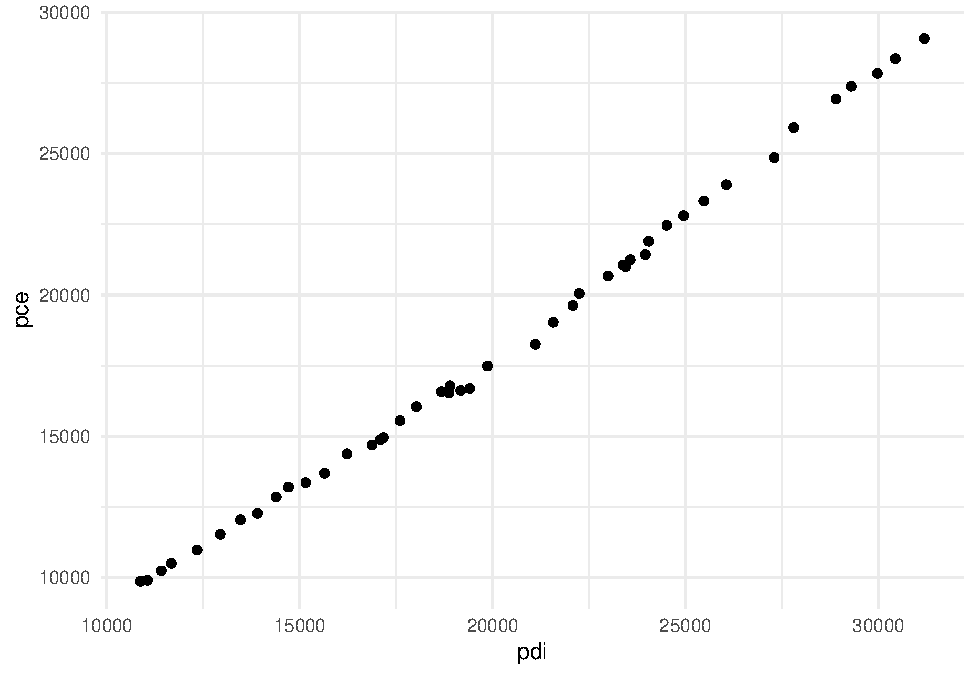
\includegraphics{rEkonometri_files/figure-latex/unnamed-chunk-13-1.pdf}

Modelin çıktısına da ulaşalım.

\begin{Shaded}
\begin{Highlighting}[]
\NormalTok{model <-}\StringTok{ }\KeywordTok{lm}\NormalTok{(}\DataTypeTok{formula =}\NormalTok{ pce }\OperatorTok{~}\StringTok{ }\NormalTok{pdi, }\DataTypeTok{data =}\NormalTok{ df_train)}
\KeywordTok{summary}\NormalTok{(model)}
\end{Highlighting}
\end{Shaded}

\begin{verbatim}
## 
## Call:
## lm(formula = pce ~ pdi, data = df_train)
## 
## Residuals:
##     Min      1Q  Median      3Q     Max 
## -789.30 -284.75  -12.24  291.49  592.29 
## 
## Coefficients:
##               Estimate Std. Error t value Pr(>|t|)    
## (Intercept) -1.084e+03  1.940e+02  -5.589 1.44e-06 ***
## pdi          9.538e-01  9.233e-03 103.298  < 2e-16 ***
## ---
## Signif. codes:  0 '***' 0.001 '**' 0.01 '*' 0.05 '.' 0.1 ' ' 1
## 
## Residual standard error: 353.5 on 43 degrees of freedom
## Multiple R-squared:  0.996,  Adjusted R-squared:  0.9959 
## F-statistic: 1.067e+04 on 1 and 43 DF,  p-value: < 2.2e-16
\end{verbatim}

pdi'daki 1 \$'lık artış pce'de 0.95 \$'lık artışa neden oluyor. Dolayısıyla marjinal tüketim eğilimi 0.95'tir.

Çıktıda da görebileceğimiz gibi modeli yaklaşık olarak \(\hat{pce_t} = -1083.98 + 0.95pdi_t\) bulduk.

Öngörüde bulunmadan önce bazı terimleri bilmemiz gerekiyor.

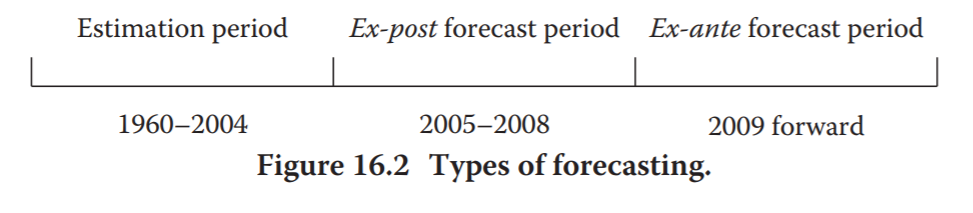
\includegraphics[width=1\linewidth]{C:/Users/datanerd/Desktop/Github/rEkonometri/img/typesofforecasting}

Nokta ve aralık öngörüleri: Noktada her öngörü dönemi için tek bir değer bulunur. Aralıkta ise belli bir olasılık ile alt ve üst sınırlar vardır. Aralık öngörü için Merkez Bankası'ndan örnek verebiliriz.

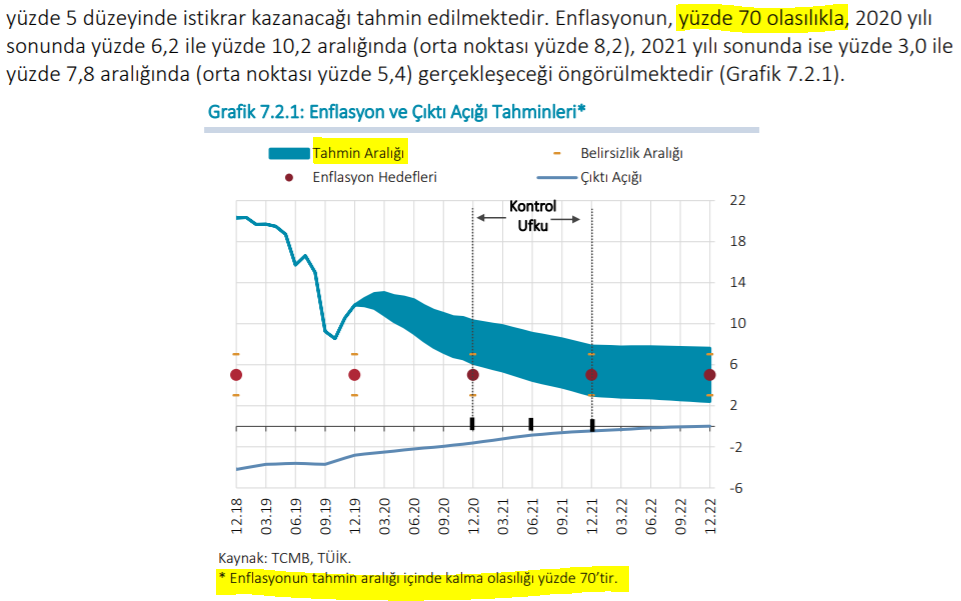
\includegraphics[width=1\linewidth]{C:/Users/datanerd/Desktop/Github/rEkonometri/img/interval}

Gerçekleşen ve öncül öngörüler (ex post and ex ante forecasts): Örneğimizde 1960-2004 yıllarını alıp model kurmuştuk. Bu tahmin dönemidir (estimation period). Gerçekleşen öngörü (ex post forecast) döneminde ise bağımlı-bağımsız değişken değerlerini biliriz. 2005-2008 yılları ayırdığımız dönemlerdir. Bu değerleri aslında biliyoruz. Bu dönem performans ölçümü ile alakalıdır. Son olarak öncül öngörüde (ex ante forecast) bağımlı değişken değerlerini tahmin döneminin ilerisi için tahmin ederiz.

\begin{Shaded}
\begin{Highlighting}[]
\NormalTok{df }\OperatorTok\StringTok{ }
\StringTok{  }\KeywordTok{filter}\NormalTok{(year }\OperatorTok\StringTok{ }\KeywordTok{c}\NormalTok{(}\DecValTok{2005}\OperatorTok{:}\DecValTok{2008}\NormalTok{)) }\OperatorTok\StringTok{ }
\StringTok{  }\NormalTok{dplyr}\OperatorTok{::}\KeywordTok{select}\NormalTok{(pdi, pce, year)}
\end{Highlighting}
\end{Shaded}

\begin{verbatim}
## # A tibble: 4 x 3
##     pdi   pce  year
##   <dbl> <dbl> <dbl>
## 1 31318 29771  2005
## 2 32271 30341  2006
## 3 32648 30838  2007
## 4 32514 30479  2008
\end{verbatim}

31,318 milyar \$ olan 2005 yılı kişi başı pdi değeri verildiğinde yine 2005 yılı için pce nedir? Burada nokta öngörü yapacağız. Kişi başı pdi verildiğinde \emph{en iyi ortalama kestirimi} elde ederiz.

\(\hat{pce}_{2005} = \beta_1 + \beta_2pdi_{2005} = -1083.98 + 0.95*31318 = 28668.12\)

31,318 milyar \$ olan pdi verildiğinde 2005 için en iyi ortalama kestirim değeri 28,668 milyar \$'dır. Biz bunun gerçek değerinin 29,771 milyar \$ olduğunu biliyoruz. Yani, öngörü hatamız (forecast error) 1,103 milyar \$'dır.

Peki, muhtemel öngörü hatamızı hesaplayabilir miyiz? Hata terimi normal dağılımlı ise\ldots{}

2005 yılı için;

\(Pr[\hat{Y}_{2005} - t_{\alpha/2}sh(\hat{Y}_{2005}) \le E(Y_{2005}) \le \hat{Y}_{2005} + t_{\alpha/2}sh(\hat{Y}_{2005})] = \%95\)

\(\alpha = \%5\)

sh: Standart hata

Normal dağılım yerine t dağılımını kullandık. Çünkü gerçek hata varyansını tahmin etmek istiyoruz.

\begin{Shaded}
\begin{Highlighting}[]
\KeywordTok{predict}\NormalTok{(model, }\DataTypeTok{newdata =} \KeywordTok{data.frame}\NormalTok{(}\DataTypeTok{pdi =} \DecValTok{31318}\NormalTok{, }\DataTypeTok{year =} \DecValTok{2005}\NormalTok{), }\DataTypeTok{interval =} \StringTok{"confidence"}\NormalTok{)}
\end{Highlighting}
\end{Shaded}

\begin{verbatim}
##        fit      lwr      upr
## 1 28786.14 28553.71 29018.57
\end{verbatim}

En iyi tek tahmin 28,786 milyar \$ olmasına rağmen \%95 güven aralığı 28,553;29,018 milyar \$ şeklindedir. Tabi biz bunu sadece 2005 için yapmayacağız. Her bir yıl için yaptığımızda ortaya bir güven bandı çıkacaktır.

\begin{Shaded}
\begin{Highlighting}[]
\NormalTok{df }\OperatorTok\StringTok{ }
\StringTok{  }\NormalTok{dplyr}\OperatorTok{::}\KeywordTok{select}\NormalTok{(pdi,year) }\OperatorTok\StringTok{ }
\StringTok{  }\KeywordTok{filter}\NormalTok{(year }\OperatorTok\StringTok{ }\KeywordTok{c}\NormalTok{(}\DecValTok{2005}\OperatorTok{:}\DecValTok{2008}\NormalTok{)) ->}\StringTok{ }\NormalTok{expost}

\KeywordTok{predict}\NormalTok{(model, }\DataTypeTok{newdata =}\NormalTok{ expost, }\DataTypeTok{interval =} \StringTok{"confidence"}\NormalTok{)}
\end{Highlighting}
\end{Shaded}

\begin{verbatim}
##        fit      lwr      upr
## 1 28786.14 28553.71 29018.57
## 2 29695.08 29446.73 29943.43
## 3 30054.65 29799.94 30309.36
## 4 29926.85 29674.40 30179.29
\end{verbatim}

Bağımsız değişken ortalama değerden uzaklaştıkça öngörü hatası artacaktır. Bu da bandın genişlemesine yol açacaktır (Merkez Bankası'nın güven bandına tekrar bakın).

Bu yazıda öngörü konusuna odaklandığımız için sahte regresyon, otokorelasyon gibi karşımıza çıkabilecek sorunları atladık.

\hypertarget{francis-galton-ve-regresyon-terimi}{%
\chapter{Francis Galton ve Regresyon Terimi}\label{francis-galton-ve-regresyon-terimi}}

Regresyon terimi ilk kez Francis Galton tarafından kullanılmıştır.

Saymak ve ölçmek Galton'ın hobisiymiş. Bırakın hobiyi saplantı da denilebilir.

\begin{quote}
\emph{Wherever you can, count.}
\end{quote}

Yapabildiğin her yerde say. Kendisi hakkında yazılan çok şey var. Gerçekten de yapabildiği her yerde saymış.

\begin{quote}
\emph{He even made a beauty map of britain, based on a secret grading of the local women on a scale from attractive to repulsive (the low point was in aberdeen).} -BBC
\end{quote}

Sokakta yürürken karşılaştığı kızları çekicilik derecelerine göre sınıflandırmış, kız alımlıysa sol cebinde taşıdığı kartı, sıradansa sağ cebindekini işaretlermiş. Böyle böyle İngiltere'nin güzellik haritasını çıkarmış ve Londralı kızlar en yüksek puanı; Aberdeenli kızlar ise son sırayı almış.

Kurduğu Galton Antropometrik (antropolojik ölçüm) Laboratuvarı'nda parmak izleri dahil insan vücuduyla ilgili mümkün olan her ölçümü yapmış, bu ölçümlerin yelpazesini ve karakterini izleyerek kaydını tutmuş. Parmak izleri Galton'ı büyülüyormuş. Nedeni ise vücudun diğer kısımlarından farklı olarak parmak izlerinin şeklinin kişi yaşlansa da hiçbir zaman değişmemesi. Galton bu konuda 200 sayfalık bir kitap yayınlamış ve bu çalışması kısa zamanda polisin parmak izini yaygın biçimde kullanmasına öncülük etmiş.

Galton, Britanya Bilimi İlerletme Birliği Başkanlığı'na seçilmesi sebebiyle bir konuşma yapar ve bu konuşma sırasında gerçekleştirdiği bir deneyde ortalamaya dönüşü destekleyen yeni kanıtlar bulduğunu açıklar. Bu deney için ise kendisine veri sağlayacak kişilere nakit ödeme yapacağını ilan eder ve insanlarla ilgili muazzam miktarda veri toplar: 205 ebeveynden doğmuş 928 yetişkin çocuk.

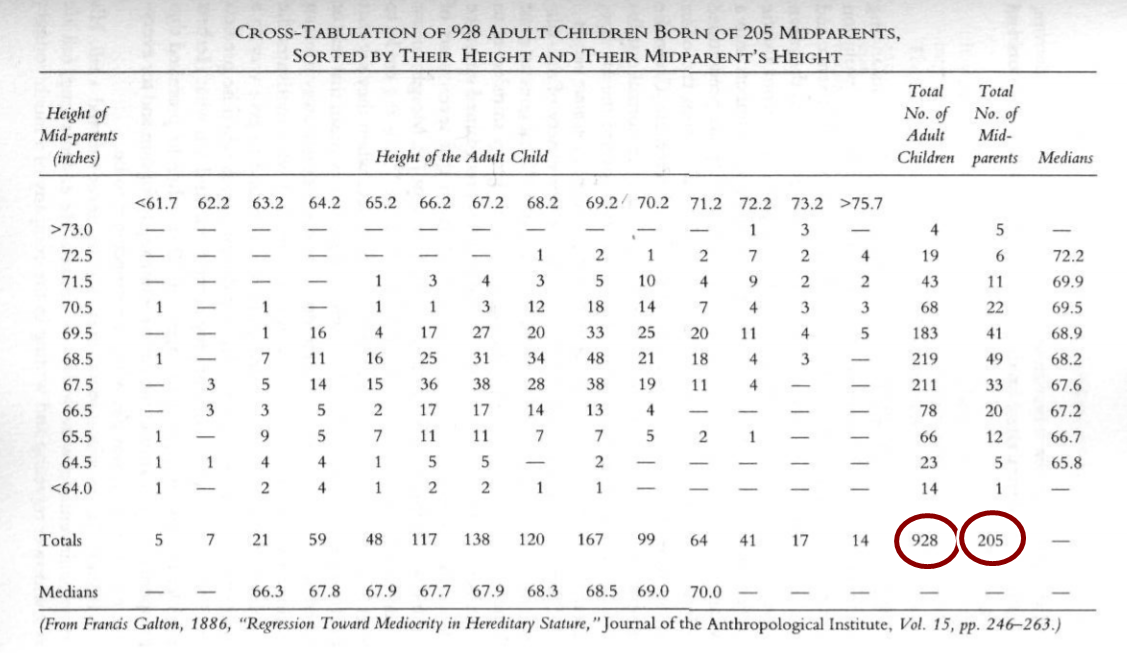
\includegraphics[width=1\linewidth]{C:/Users/datanerd/Desktop/Github/rEkonometri/img/galton_tablo}

R ile verilere ulaşabilmek mümkündür.

\begin{Shaded}
\begin{Highlighting}[]
\KeywordTok{library}\NormalTok{(HistData);}\KeywordTok{library}\NormalTok{(tidyverse)}

\NormalTok{Galton }\OperatorTok\StringTok{ }
\StringTok{  }\KeywordTok{ggplot}\NormalTok{(}\KeywordTok{aes}\NormalTok{(}\DataTypeTok{x=}\NormalTok{parent, }\DataTypeTok{y=}\NormalTok{child)) }\OperatorTok{+}
\StringTok{  }\KeywordTok{geom_point}\NormalTok{(}\DataTypeTok{color=}\StringTok{"red"}\NormalTok{) }\OperatorTok{+}
\StringTok{  }\KeywordTok{geom_smooth}\NormalTok{(}\DataTypeTok{method =} \StringTok{"lm"}\NormalTok{, }\DataTypeTok{color=}\StringTok{"black"}\NormalTok{, }\DataTypeTok{se=}\OtherTok{FALSE}\NormalTok{) }\OperatorTok{+}
\StringTok{  }\KeywordTok{scale_y_continuous}\NormalTok{(}\DataTypeTok{limits =} \KeywordTok{c}\NormalTok{(}\DecValTok{55}\NormalTok{,}\DecValTok{80}\NormalTok{)) }\OperatorTok{+}
\StringTok{  }\KeywordTok{theme_minimal}\NormalTok{()}
\end{Highlighting}
\end{Shaded}

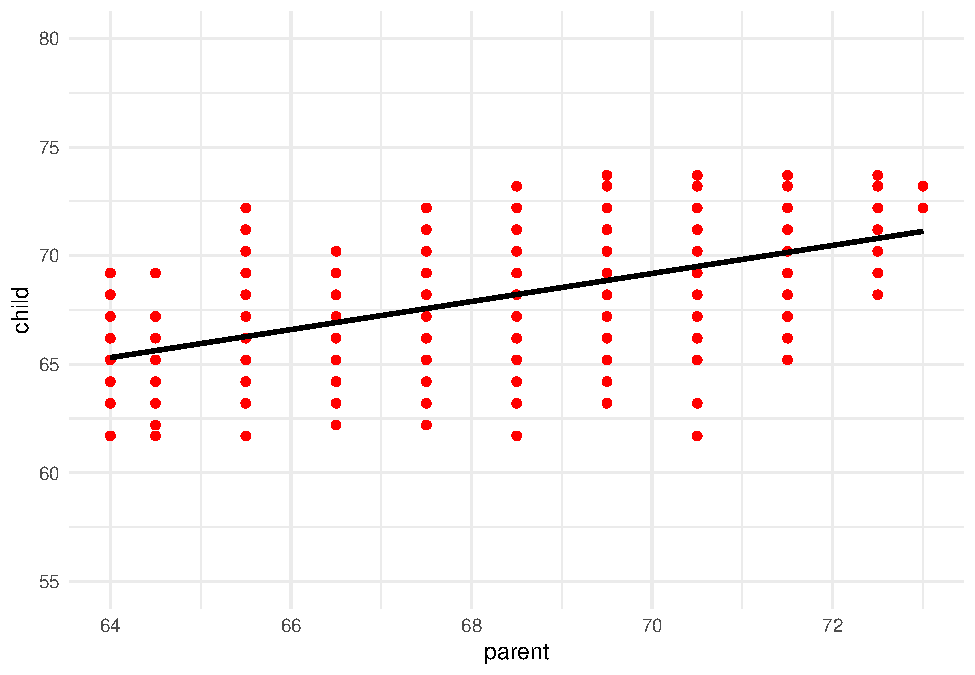
\includegraphics{rEkonometri_files/figure-latex/unnamed-chunk-21-1.pdf}

Gözlemleri inceleyebilmek için kadınlar ve erkekler arasındaki boy farklarıyla ilgili bir düzeltme yapar. Bunun için bütün annelerin boylarını 1.08 ile çarpar, ardından da anne ve babaların boylarını toplayıp ikiye böler. Elde ettiği birime de \emph{orta ebeveyn boyu} adını verir. Tabi bu arada uzunlar uzunlarla, kısalar kısalarla evleniyor gibi bir eğilim var mı diye de hesaplamalar yapar ama böyle bir eğilimin bulunmadığını varsayacağı noktaya yeterince yakındır.

Tabloda\ldots{} Sayıların sol alt köşeden sağ üst köşeye çarpraz bir yapı segilediğini görüyoruz. Yani, uzun boylu ebeveynlerin uzun boylu, kısa boylu ebeveynlerin de kısa boylu çocukları olduğunu gösteriyor: Kalıtım. Büyük sayıların ise tablonun ortasında toplandığı görülebilir. Bu ise her boy grubunun çocuklar arasında normal dağıldığını, aynı şekilde aynı ebeveynlerle ilgili her boy grubundan her çocuk dizisinin de, normal bir dağılım gösterdiğini söyler.

\begin{quote}
\emph{I never felt such a glow of loyalty and respect towards the sovereignty and magnificent sway of mathematical analysis.}
\end{quote}

Matematiksel analizin hükümranlığına ve muhteşem ruhuna hiç bu kadar derin bir bağlılık ve saygı duymamıştım der Galton.

O bizi günlük yaşama, insanların soluk aldığı, terlediği, cinsel ilişkide bulunduğu ve geleceğinden endişelendiği dünyaya götürür. Artık daha önceki matematikçilerin teorilerini doğrulama aracı olarak kullandıkları kumar masalarından da, yıldızlardan da uzaklaşmış bulunuyoruz. Galton, teorileri bulduğu şekilde ele almış ve onları neyin önemli kıldığını keşfetmeye çalışmıştır.

\hypertarget{deux11fiux15fkenleri-doux11frusal-olmayan-regresyon-modelleri}{%
\chapter{Değişkenleri Doğrusal Olmayan Regresyon Modelleri}\label{deux11fiux15fkenleri-doux11frusal-olmayan-regresyon-modelleri}}

Doğrusallığın tanımını şöyle yapmıştık:

\begin{quote}
\emph{Doğrusal dediğimiz zaman buradaki doğrusallığın değişkenlerden (X'ler) değil; parametrelerden} (\(\beta'lar\)) \emph{geldiğini bilmemiz gerekiyor. Bağımlı ve bağımsız değişken(ler) logaritmik, tersi veya kuvveti alınmış şekilde olabilir. Bu, doğrusallık kavramını etkilemez. Asıl önemli olan} \(\beta\) \emph{parametrelerinin kuvvetinin alınmaması, diğer parametrelere bölünmemesi veya dönüştürülmemesidir.}
\end{quote}

Bu başlık altında parametrelerine göre doğrusal olan ama değişkenleri açısından doğrusallık göstermeyen modellerle ilgili uygulamalar yapacağız.

\begin{Shaded}
\begin{Highlighting}[]
\KeywordTok{library}\NormalTok{(readxl);}\KeywordTok{library}\NormalTok{(tidyverse);}\KeywordTok{library}\NormalTok{(magrittr);}\KeywordTok{library}\NormalTok{(moments)}

\KeywordTok{setwd}\NormalTok{(}\StringTok{"C:/Users/datanerd/Desktop/Github/rEkonometri/data"}\NormalTok{)}
\NormalTok{df1 <-}\StringTok{ }\KeywordTok{read_excel}\NormalTok{(}\StringTok{"Table1_1.xls"}\NormalTok{)}
\NormalTok{df2 <-}\StringTok{ }\KeywordTok{read_excel}\NormalTok{(}\StringTok{"Table2_1.xls"}\NormalTok{)}
\NormalTok{df3 <-}\StringTok{ }\KeywordTok{read_excel}\NormalTok{(}\StringTok{"tepav_il_gsyh_gece_isiklari.xlsx"}\NormalTok{, }\DataTypeTok{sheet =} \StringTok{"Kişi Başına GSYH ($) Türkiye")}
\StringTok{df4 <- read_excel("}\NormalTok{Table2_}\FloatTok{8.}\NormalTok{xls}\StringTok{")}
\end{Highlighting}
\end{Shaded}

\hypertarget{log-doux11frusal-ya-da-uxe7ift-log-modeller}{%
\section{Log-Doğrusal ya da Çift-Log Modeller}\label{log-doux11frusal-ya-da-uxe7ift-log-modeller}}

Aşağıdaki modeli ele alalım.

\(Y_i = \beta_1X_i^{\beta_2}e^{\epsilon_i}\)

Her iki tarafın logaritmasını alırsak (log-doğrusal, çift-log);

\(lnY_i = ln\beta_1 + \beta_2lnX_i + \epsilon_i\)

\emph{ln: e tabanına göre logaritmadır.}

Yukarıda bir doğrusallaştırma işlemi yaptık.

\begin{Shaded}
\begin{Highlighting}[]
\NormalTok{df2 }\OperatorTok\StringTok{ }
\StringTok{  }\NormalTok{dplyr}\OperatorTok{::}\KeywordTok{select}\NormalTok{(output, capital, labor) }\OperatorTok\StringTok{ }
\StringTok{  }\KeywordTok{mutate}\NormalTok{(}\DataTypeTok{lnoutput =} \KeywordTok{log}\NormalTok{(output),}
         \DataTypeTok{lncapital =} \KeywordTok{log}\NormalTok{(capital),}
         \DataTypeTok{lnlabor =} \KeywordTok{log}\NormalTok{(labor)) }\CommentTok{#Her bir değişkenin logaritmasını aldık.}

\KeywordTok{str}\NormalTok{(df2)}
\end{Highlighting}
\end{Shaded}

\begin{verbatim}
## tibble [51 x 6] (S3: tbl_df/tbl/data.frame)
##  $ output   : num [1:51] 3.84e+07 1.81e+06 2.37e+07 2.70e+07 2.18e+08 ...
##  $ capital  : num [1:51] 2689076 57997 2308272 1376235 13554116 ...
##  $ labor    : num [1:51] 424471 19895 206893 304055 1809756 ...
##  $ lnoutput : num [1:51] 17.5 14.4 17 17.1 19.2 ...
##  $ lncapital: num [1:51] 14.8 11 14.7 14.1 16.4 ...
##  $ lnlabor  : num [1:51] 13 9.9 12.2 12.6 14.4 ...
\end{verbatim}

ABD için Cobb-Douglas üretim fonksiyonuna bakıyoruz.

Bağımlı değişken:

\begin{itemize}
\tightlist
\item
  \textbf{output:} İmalat sektörüne ait çıktı (katma değer, bin \$)
\end{itemize}

Bağımsız değişken(ler):

\begin{itemize}
\item
  \textbf{capital:} Sermaye girdisi (sermaye harcaması, bin \$)
\item
  \textbf{labor:} Emek girdisi (çalışma saati, bin saat)
\end{itemize}

Modeli kurabiliriz.

\begin{Shaded}
\begin{Highlighting}[]
\NormalTok{model <-}\StringTok{ }\KeywordTok{lm}\NormalTok{(}\DataTypeTok{formula =}\NormalTok{ lnoutput }\OperatorTok{~}\StringTok{ }\NormalTok{lncapital }\OperatorTok{+}\StringTok{ }\NormalTok{lnlabor, }\DataTypeTok{data =}\NormalTok{ df2)}
\KeywordTok{summary}\NormalTok{(model)}
\end{Highlighting}
\end{Shaded}

\begin{verbatim}
## 
## Call:
## lm(formula = lnoutput ~ lncapital + lnlabor, data = df2)
## 
## Residuals:
##      Min       1Q   Median       3Q      Max 
## -0.45645 -0.12112 -0.05319  0.04518  1.21579 
## 
## Coefficients:
##             Estimate Std. Error t value Pr(>|t|)    
## (Intercept)  3.88760    0.39623   9.812 4.70e-13 ***
## lncapital    0.52128    0.09689   5.380 2.18e-06 ***
## lnlabor      0.46833    0.09893   4.734 1.98e-05 ***
## ---
## Signif. codes:  0 '***' 0.001 '**' 0.01 '*' 0.05 '.' 0.1 ' ' 1
## 
## Residual standard error: 0.2668 on 48 degrees of freedom
## Multiple R-squared:  0.9642, Adjusted R-squared:  0.9627 
## F-statistic: 645.9 on 2 and 48 DF,  p-value: < 2.2e-16
\end{verbatim}

Çıktıya ait parametreler esnekliklerdir. Parametreleri farklı olarak şöyle yorumlayacağız: labor girdisi sabit tutulduğunda, capital girdisini \%1 artırırsak output \%0.52 artacaktır. Aynı şekilde capital girdisi sabit tutulduğunda, labor girdisini \%1 artırırsak output \%0.47 artacaktır.

p değerleri çok düşüktür. Bu da parametrelerin istatistiksel olarak anlamlı olduğu ve output üzerinde etkiye sahip olduklarını gösterir.

F ve onun p değerine bakarsak capital ve labor değişkenlerinin bir arada istatistiksel olarak anlamlı olduğunu görürüz. Bu da en az birinin output üzerinde etkisinin olduğunu gösterir.

\(R^2\) değerleri \%96 ile oldukça yüksektir.

Peki, değişkenlerin logaritmasını almadan model kursaydık ne olurdu?

\begin{Shaded}
\begin{Highlighting}[]
\NormalTok{model <-}\StringTok{ }\KeywordTok{lm}\NormalTok{(}\DataTypeTok{formula =}\NormalTok{ output }\OperatorTok{~}\StringTok{ }\NormalTok{capital }\OperatorTok{+}\StringTok{ }\NormalTok{labor, }\DataTypeTok{data =}\NormalTok{ df2)}
\KeywordTok{summary}\NormalTok{(model)}
\end{Highlighting}
\end{Shaded}

\begin{verbatim}
## 
## Call:
## lm(formula = output ~ capital + labor, data = df2)
## 
## Residuals:
##      Min       1Q   Median       3Q      Max 
## -9397412 -4258427  -722360  1573961 21015574 
## 
## Coefficients:
##              Estimate Std. Error t value Pr(>|t|)    
## (Intercept) 2.336e+05  1.250e+06   0.187    0.853    
## capital     9.952e+00  9.781e-01  10.175 1.43e-13 ***
## labor       4.799e+01  7.058e+00   6.799 1.50e-08 ***
## ---
## Signif. codes:  0 '***' 0.001 '**' 0.01 '*' 0.05 '.' 0.1 ' ' 1
## 
## Residual standard error: 6301000 on 48 degrees of freedom
## Multiple R-squared:  0.9811, Adjusted R-squared:  0.9803 
## F-statistic:  1244 on 2 and 48 DF,  p-value: < 2.2e-16
\end{verbatim}

capital ve labor parametreleri istatistiksel olarak anlamlıdır (kesme terimi hariç) fakat yorumları yukarıdaki gibi olmayacaktır.

labor girdisi sabit tutulduğunda, capital girdisindeki 1 birimlik artışın output üzerindeki ortalama etkisi 10 birimdir. capital girdisi sabit tutulduğunda, labor girdisindeki 1 birimlik artışın ise output üzerindeki ortalama etkisi 48 birimdir.

\hypertarget{log-lin-ya-da-yarux131-logaritmik-modeller}{%
\section{Log-Lin ya da Yarı-Logaritmik Modeller}\label{log-lin-ya-da-yarux131-logaritmik-modeller}}

Bu modellerde, bağımsız değişkendeki bir birim değişime karşılık bağımlı değişkendeki yüzde büyümeyi bulmak ile ilgileniriz.

\begin{Shaded}
\begin{Highlighting}[]
\NormalTok{df3 }\OperatorTok\StringTok{ }
\StringTok{  }\KeywordTok{mutate}\NormalTok{(}\DataTypeTok{lnkbgsyh =} \KeywordTok{log}\NormalTok{(kbgsyh)) }\CommentTok{#Bağımlı değişkenin logaritması alındı.}

\KeywordTok{str}\NormalTok{(df3)}
\end{Highlighting}
\end{Shaded}

\begin{verbatim}
## tibble [27 x 4] (S3: tbl_df/tbl/data.frame)
##  $ yıllar  : num [1:27] 1992 1993 1994 1995 1996 ...
##  $ kbgsyh  : num [1:27] 3720 4159 3048 3842 4085 ...
##  $ zaman   : num [1:27] 1 2 3 4 5 6 7 8 9 10 ...
##  $ lnkbgsyh: num [1:27] 8.22 8.33 8.02 8.25 8.32 ...
\end{verbatim}

Türkiye'ye ait veriler, TEPAV'ın yaptığı \emph{1992-2018 Dönemi için Gece Işıklarıyla İl Bazında GSYH Tahmini: 2018'de 81 İlin Büyüme Performansı} başlıklı çalışmasından elde edilmiştir.

\begin{Shaded}
\begin{Highlighting}[]
\NormalTok{df3 }\OperatorTok\StringTok{ }
\StringTok{  }\KeywordTok{ggplot}\NormalTok{(}\KeywordTok{aes}\NormalTok{(}\DataTypeTok{x =}\NormalTok{ zaman, }\DataTypeTok{y =}\NormalTok{ kbgsyh)) }\OperatorTok{+}
\StringTok{  }\KeywordTok{geom_line}\NormalTok{() }\OperatorTok{+}
\StringTok{  }\KeywordTok{theme_minimal}\NormalTok{()}
\end{Highlighting}
\end{Shaded}

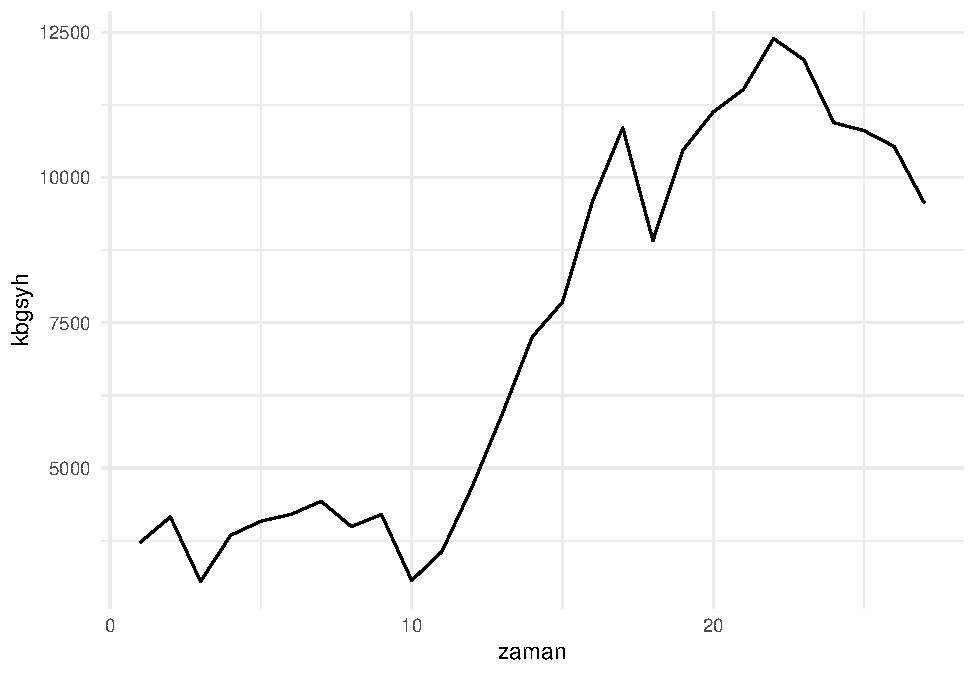
\includegraphics{rEkonometri_files/figure-latex/unnamed-chunk-27-1.pdf}

Bağımlı değişken:

\begin{itemize}
\tightlist
\item
  \textbf{kbgsyh:} Kişi Başına GSYH
\end{itemize}

Bağımsız değişken(ler):

\begin{itemize}
\tightlist
\item
  \textbf{zaman:} Zaman
\end{itemize}

Modeli kuralım.

\begin{Shaded}
\begin{Highlighting}[]
\NormalTok{model <-}\StringTok{ }\KeywordTok{lm}\NormalTok{(}\DataTypeTok{formula =}\NormalTok{ lnkbgsyh }\OperatorTok{~}\StringTok{ }\NormalTok{zaman, }\DataTypeTok{data =}\NormalTok{ df3)}
\KeywordTok{summary}\NormalTok{(model)}
\end{Highlighting}
\end{Shaded}

\begin{verbatim}
## 
## Call:
## lm(formula = lnkbgsyh ~ zaman, data = df3)
## 
## Residuals:
##      Min       1Q   Median       3Q      Max 
## -0.52483 -0.13965  0.04205  0.17764  0.34329 
## 
## Coefficients:
##             Estimate Std. Error t value Pr(>|t|)    
## (Intercept) 7.984766   0.087808   90.93  < 2e-16 ***
## zaman       0.056749   0.005481   10.35 1.58e-10 ***
## ---
## Signif. codes:  0 '***' 0.001 '**' 0.01 '*' 0.05 '.' 0.1 ' ' 1
## 
## Residual standard error: 0.2218 on 25 degrees of freedom
## Multiple R-squared:  0.8109, Adjusted R-squared:  0.8033 
## F-statistic: 107.2 on 1 and 25 DF,  p-value: 1.581e-10
\end{verbatim}

1992-2018 döneminde Türkiye kbgsyh'sinin yıllık \%5.67 büyüdüğünü söyleyebiliriz. zaman'ın p değeri oldukça düşüktür ve istatistiksel olarak anlamlıdır. Bu parametre anlık büyüme hızını verir; bileşik büyüme hızını değil. Eğer ters logaritmasını alıp 1 çıkarırsak bileşik büyüme hızına da ulaşabiliriz ki bu da \%5.84'tür.

\begin{Shaded}
\begin{Highlighting}[]
\KeywordTok{exp}\NormalTok{(}\KeywordTok{as.numeric}\NormalTok{(model}\OperatorTok{$}\NormalTok{coefficients[}\DecValTok{2}\NormalTok{])) }\OperatorTok{-}\StringTok{ }\DecValTok{1}
\end{Highlighting}
\end{Shaded}

\begin{verbatim}
## [1] 0.05839053
\end{verbatim}

Kesme teriminin ters logaritmasını alırsak aşağıdaki değeri bulacağız. Bu, kbgsyh'nin başlangıç (1992 yılı) değeridir. 1992 için gerçek kbgsyh 3720 \$'dır.

\begin{Shaded}
\begin{Highlighting}[]
\KeywordTok{exp}\NormalTok{(}\KeywordTok{as.numeric}\NormalTok{(model}\OperatorTok{$}\NormalTok{coefficients[}\DecValTok{1}\NormalTok{]))}
\end{Highlighting}
\end{Shaded}

\begin{verbatim}
## [1] 2935.891
\end{verbatim}

\begin{Shaded}
\begin{Highlighting}[]
\NormalTok{df3}\OperatorTok{$}\NormalTok{kbgsyh[}\DecValTok{1}\NormalTok{] }\CommentTok{#Başlangıç 1992 yılıdır.}
\end{Highlighting}
\end{Shaded}

\begin{verbatim}
## [1] 3720.399
\end{verbatim}

Burada doğrusal trend modeli de kurulabilirdi.

\begin{Shaded}
\begin{Highlighting}[]
\NormalTok{model <-}\StringTok{ }\KeywordTok{lm}\NormalTok{(}\DataTypeTok{formula =}\NormalTok{ kbgsyh }\OperatorTok{~}\StringTok{ }\NormalTok{zaman, }\DataTypeTok{data =}\NormalTok{ df3)}
\KeywordTok{summary}\NormalTok{(model)}
\end{Highlighting}
\end{Shaded}

\begin{verbatim}
## 
## Call:
## lm(formula = kbgsyh ~ zaman, data = df3)
## 
## Residuals:
##      Min       1Q   Median       3Q      Max 
## -2702.26  -990.27   -25.07  1353.35  2422.91 
## 
## Coefficients:
##             Estimate Std. Error t value Pr(>|t|)    
## (Intercept)  1930.27     588.50    3.28  0.00305 ** 
## zaman         382.72      36.73   10.42 1.39e-10 ***
## ---
## Signif. codes:  0 '***' 0.001 '**' 0.01 '*' 0.05 '.' 0.1 ' ' 1
## 
## Residual standard error: 1487 on 25 degrees of freedom
## Multiple R-squared:  0.8128, Adjusted R-squared:  0.8053 
## F-statistic: 108.6 on 1 and 25 DF,  p-value: 1.392e-10
\end{verbatim}

zaman değişkeni trend değişkendir. zaman'ın eğim parametresi birim dönemde kbgsyh'deki mutlak değişimi verir. Bu parametre pozitif ise yükselen; negatif ise azalan trend anlamını taşır.

Sonuçlar 1992-2018 yılı boyunca Türkiye'de Kişi Başına GSYH'nin yıllık 383 \$ arttığını söyler. Bu da yükselen bir trend olduğunu gösterir.

\hypertarget{lin-log-modeller}{%
\section{Lin-Log Modeller}\label{lin-log-modeller}}

Bu modeller, bağımsız değişkendeki yüzde değişime karşılık bağımlı değişkendeki mutlak değişimin ölçüsü nedir sorusuna cevap verir.

\begin{Shaded}
\begin{Highlighting}[]
\NormalTok{df4 }\OperatorTok\StringTok{ }
\StringTok{  }\NormalTok{dplyr}\OperatorTok{::}\KeywordTok{select}\NormalTok{(expend, sfdho) }\OperatorTok\StringTok{ }
\StringTok{  }\KeywordTok{mutate}\NormalTok{(}\DataTypeTok{lnexpend =} \KeywordTok{log}\NormalTok{(expend)) }\CommentTok{#Bağımsız değişkenin logaritması alındı.}

\KeywordTok{str}\NormalTok{(df4)}
\end{Highlighting}
\end{Shaded}

\begin{verbatim}
## tibble [869 x 3] (S3: tbl_df/tbl/data.frame)
##  $ expend  : num [1:869] 40517 33541 5182 40385 40302 ...
##  $ sfdho   : num [1:869] 0.1598 0.0938 0.3149 0.0596 0.0553 ...
##  $ lnexpend: num [1:869] 10.61 10.42 8.55 10.61 10.6 ...
\end{verbatim}

ABD hanehalkı için evde tüketilen yiyecek ve alkolsüz içecekler ile toplam hanehalkı harcamasına ait verilere bakıyoruz.

Bağımlı değişken:

\begin{itemize}
\tightlist
\item
  \textbf{sfdho:} Gıda harcamasının toplam harcamadaki payı
\end{itemize}

Bağımsız değişken(ler):

\begin{itemize}
\tightlist
\item
  \textbf{expend:} Toplam hanehalkı harcaması
\end{itemize}

Modeli kuralım.

\begin{Shaded}
\begin{Highlighting}[]
\NormalTok{model <-}\StringTok{ }\KeywordTok{lm}\NormalTok{(}\DataTypeTok{formula =}\NormalTok{ sfdho }\OperatorTok{~}\StringTok{ }\NormalTok{lnexpend, }\DataTypeTok{data =}\NormalTok{ df4)}
\KeywordTok{summary}\NormalTok{(model)}
\end{Highlighting}
\end{Shaded}

\begin{verbatim}
## 
## Call:
## lm(formula = sfdho ~ lnexpend, data = df4)
## 
## Residuals:
##      Min       1Q   Median       3Q      Max 
## -0.18180 -0.04350 -0.00654  0.03373  0.48594 
## 
## Coefficients:
##              Estimate Std. Error t value Pr(>|t|)    
## (Intercept)  0.930387   0.036367   25.58   <2e-16 ***
## lnexpend    -0.077737   0.003591  -21.65   <2e-16 ***
## ---
## Signif. codes:  0 '***' 0.001 '**' 0.01 '*' 0.05 '.' 0.1 ' ' 1
## 
## Residual standard error: 0.06875 on 867 degrees of freedom
## Multiple R-squared:  0.3509, Adjusted R-squared:  0.3501 
## F-statistic: 468.6 on 1 and 867 DF,  p-value: < 2.2e-16
\end{verbatim}

Tahmin edilen parametrelere ait p değerleri oldukça düşüktür ya da istatistiksel olarak anlamlıdır.

Toplam harcama \%1 arttığında yiyecek ve alkolsüz içeceklerin harcamadaki payı ortalama 0.0008 birim düşecektir ama parametre -0.08? Bu modellerde doğru yorumlamak için eğim parametresi 100'e bölünür. Alternatif olarak şu yorum da yapılabilir: Toplam harcama \%100 arttığında yiyecek ve alkolsüz içeceklerin harcamadaki payı 0.08 birim azalır.

\hypertarget{ters-modeller}{%
\section{Ters Modeller}\label{ters-modeller}}

Bazen bağımlı değişken ile bağımsız değişkenler arasında ters yönlü ilişki olabilir.

\begin{Shaded}
\begin{Highlighting}[]
\KeywordTok{ggplot}\NormalTok{(df4, }\KeywordTok{aes}\NormalTok{(}\DataTypeTok{x =}\NormalTok{ lnexpend, }\DataTypeTok{y =}\NormalTok{ sfdho)) }\OperatorTok{+}
\StringTok{  }\KeywordTok{geom_point}\NormalTok{() }\OperatorTok{+}
\StringTok{  }\KeywordTok{theme_minimal}\NormalTok{()}
\end{Highlighting}
\end{Shaded}

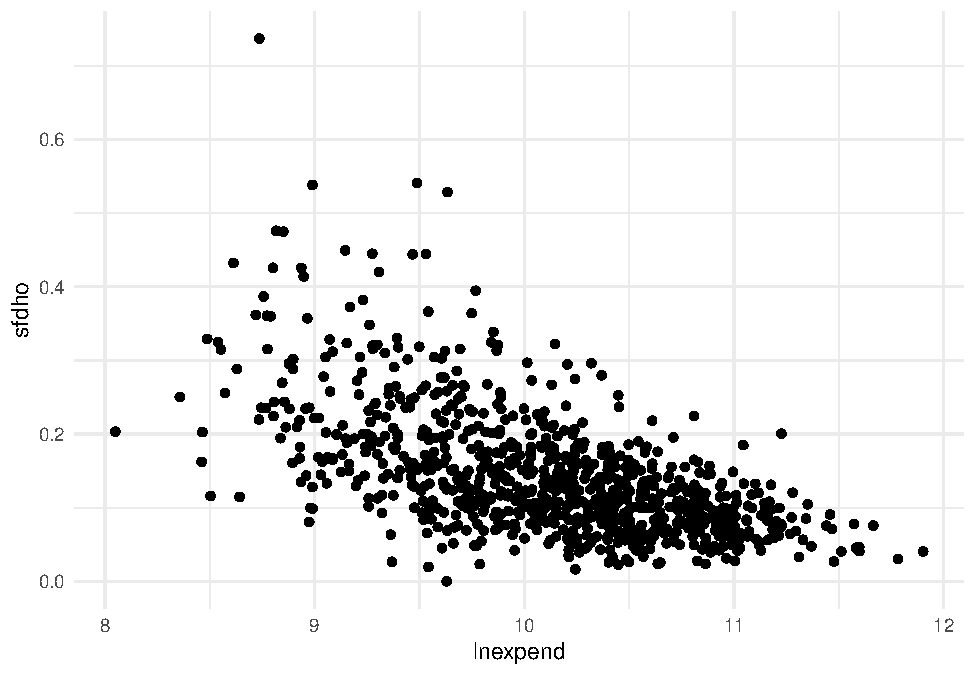
\includegraphics{rEkonometri_files/figure-latex/unnamed-chunk-34-1.pdf}

\begin{Shaded}
\begin{Highlighting}[]
\NormalTok{df4 }\OperatorTok\StringTok{ }
\StringTok{  }\KeywordTok{mutate}\NormalTok{(}\DataTypeTok{expend_ters =} \DecValTok{1} \OperatorTok{/}\StringTok{ }\NormalTok{expend) }\CommentTok{#expend değişkenini 1 / expend (expend_ters) olarak çevirdik.}
\end{Highlighting}
\end{Shaded}

Modeli kuralım.

\begin{Shaded}
\begin{Highlighting}[]
\NormalTok{model <-}\StringTok{ }\KeywordTok{lm}\NormalTok{(}\DataTypeTok{formula =}\NormalTok{ sfdho }\OperatorTok{~}\StringTok{ }\NormalTok{expend_ters, }\DataTypeTok{data =}\NormalTok{ df4)}
\KeywordTok{summary}\NormalTok{(model)}
\end{Highlighting}
\end{Shaded}

\begin{verbatim}
## 
## Call:
## lm(formula = sfdho ~ expend_ters, data = df4)
## 
## Residuals:
##      Min       1Q   Median       3Q      Max 
## -0.29889 -0.04205 -0.01120  0.03229  0.44606 
## 
## Coefficients:
##              Estimate Std. Error t value Pr(>|t|)    
## (Intercept) 7.726e-02  4.012e-03   19.26   <2e-16 ***
## expend_ters 1.331e+03  6.396e+01   20.82   <2e-16 ***
## ---
## Signif. codes:  0 '***' 0.001 '**' 0.01 '*' 0.05 '.' 0.1 ' ' 1
## 
## Residual standard error: 0.06968 on 867 degrees of freedom
## Multiple R-squared:  0.3332, Adjusted R-squared:  0.3325 
## F-statistic: 433.3 on 1 and 867 DF,  p-value: < 2.2e-16
\end{verbatim}

Parametreler istatistiksel olarak anlamlıdır. 0.08 olan kesme terimi, toplam harcama sonsuza gittiğinde yiyecek ve alkolsüz içecek harcamasının toplam harcamadaki payının er ya da geç \%8'e yerleşeceğini belirtir. expend\_ters pozitiftir. Yani, sfdho'nun toplam harcamaya göre değişim hızının her noktada negatif olacağını belirtir. Bunu grafikle gösterebiliriz.

\begin{Shaded}
\begin{Highlighting}[]
\KeywordTok{ggplot}\NormalTok{(df4, }\KeywordTok{aes}\NormalTok{(}\DataTypeTok{x =}\NormalTok{ expend, }\DataTypeTok{y =}\NormalTok{ sfdho)) }\OperatorTok{+}
\StringTok{  }\KeywordTok{geom_point}\NormalTok{() }\OperatorTok{+}
\StringTok{  }\KeywordTok{theme_minimal}\NormalTok{()}
\end{Highlighting}
\end{Shaded}

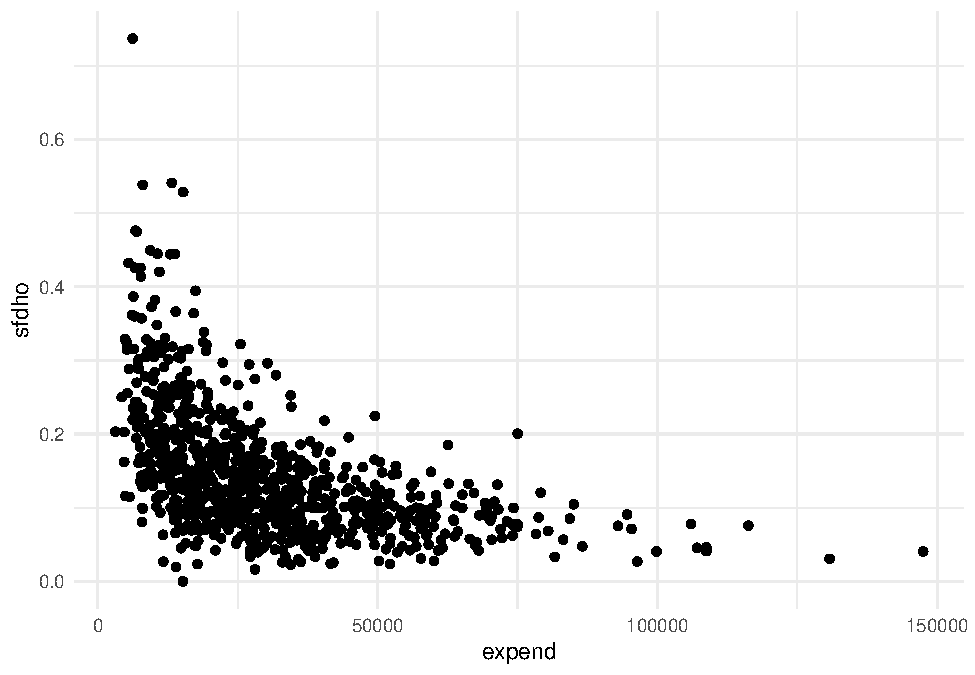
\includegraphics{rEkonometri_files/figure-latex/unnamed-chunk-37-1.pdf}

\hypertarget{polinom-regresyon-modelleri}{%
\section{Polinom Regresyon Modelleri}\label{polinom-regresyon-modelleri}}

Doğrusal trend modelinde kbgsyh'nin zaman'a göre regresyonunu almıştık. Şimdi, zamanın doğrusal olmayan bir fonksiyonu olan zaman'ın karesini alacağız ve karesel fonksiyon ya da ikinci dereceden polinoma döneceğiz (Bağımsız değişkenin en büyük kuvveti ne ise polinomun derecesi odur). zaman ve zaman'ın karesi çoklu doğrusallık sorunu yaratmaz. Nedeni ise zaman'ın karesinin zamanın doğrusal olmayan bir fonksiyonu olmasıdır.

Modeli kuralım.

\begin{Shaded}
\begin{Highlighting}[]
\NormalTok{model <-}\StringTok{ }\KeywordTok{lm}\NormalTok{(}\DataTypeTok{formula =}\NormalTok{ kbgsyh }\OperatorTok{~}\StringTok{ }\NormalTok{zaman }\OperatorTok{+}\StringTok{ }\KeywordTok{I}\NormalTok{(zaman}\OperatorTok{^}\DecValTok{2}\NormalTok{), }\DataTypeTok{data =}\NormalTok{ df3)}
\KeywordTok{summary}\NormalTok{(model)}
\end{Highlighting}
\end{Shaded}

\begin{verbatim}
## 
## Call:
## lm(formula = kbgsyh ~ zaman + I(zaman^2), data = df3)
## 
## Residuals:
##      Min       1Q   Median       3Q      Max 
## -2744.20  -973.95    -5.67  1328.45  2442.91 
## 
## Coefficients:
##              Estimate Std. Error t value Pr(>|t|)  
## (Intercept) 1982.6577   945.0924   2.098   0.0466 *
## zaman        371.8857   155.5635   2.391   0.0250 *
## I(zaman^2)     0.3871     5.3921   0.072   0.9434  
## ---
## Signif. codes:  0 '***' 0.001 '**' 0.01 '*' 0.05 '.' 0.1 ' ' 1
## 
## Residual standard error: 1517 on 24 degrees of freedom
## Multiple R-squared:  0.8128, Adjusted R-squared:  0.7973 
## F-statistic: 52.12 on 2 and 24 DF,  p-value: 1.846e-09
\end{verbatim}

\(zaman^2\) dışında parametreler istatistiksel olarak anlamlıdır.

\(zaman^2\) istatistiksel olarak anlamlı olsaydı\ldots{} Karesel model için kbgsyh artan bir oranda artmaktadır derdik. Çünkü zaman ve \(zaman^2\) değişkenlerinin parametre işaretleri pozitiftir.

Mesela bir de karesel trend değişkenli Log-Lin modeli kuralım.

\begin{Shaded}
\begin{Highlighting}[]
\NormalTok{model <-}\StringTok{ }\KeywordTok{lm}\NormalTok{(}\DataTypeTok{formula =}\NormalTok{ lnkbgsyh }\OperatorTok{~}\StringTok{ }\NormalTok{zaman }\OperatorTok{+}\StringTok{ }\KeywordTok{I}\NormalTok{(zaman}\OperatorTok{^}\DecValTok{2}\NormalTok{), }\DataTypeTok{data =}\NormalTok{ df3)}
\KeywordTok{summary}\NormalTok{(model)}
\end{Highlighting}
\end{Shaded}

\begin{verbatim}
## 
## Call:
## lm(formula = lnkbgsyh ~ zaman + I(zaman^2), data = df3)
## 
## Residuals:
##      Min       1Q   Median       3Q      Max 
## -0.53816 -0.13433  0.05264  0.17750  0.32788 
## 
## Coefficients:
##               Estimate Std. Error t value Pr(>|t|)    
## (Intercept)  7.9443909  0.1406236  56.494  < 2e-16 ***
## zaman        0.0651029  0.0231468   2.813  0.00964 ** 
## I(zaman^2)  -0.0002983  0.0008023  -0.372  0.71327    
## ---
## Signif. codes:  0 '***' 0.001 '**' 0.01 '*' 0.05 '.' 0.1 ' ' 1
## 
## Residual standard error: 0.2257 on 24 degrees of freedom
## Multiple R-squared:  0.812,  Adjusted R-squared:  0.7963 
## F-statistic: 51.83 on 2 and 24 DF,  p-value: 1.951e-09
\end{verbatim}

zaman pozitif iken \(zaman^2\) negatiftir. Bu durum kbgsyh'nin büyüme hızının pozitif olmasına rağmen azalan oranda arttığını gösterir (\(zaman^2\) istatistiksel olarak anlamlı olsaydı).

Güncel bir uygulama olarak Türkiye Covid-19 verilerini de kullanabiliriz.

\begin{Shaded}
\begin{Highlighting}[]
\NormalTok{zaman <-}\StringTok{ }\KeywordTok{seq}\NormalTok{(}\DecValTok{1}\NormalTok{,}\DecValTok{32}\NormalTok{,}\DecValTok{1}\NormalTok{)}
\NormalTok{vaka <-}\StringTok{ }\KeywordTok{c}\NormalTok{(}\DecValTok{1}\NormalTok{, }\DecValTok{1}\NormalTok{, }\DecValTok{5}\NormalTok{, }\DecValTok{5}\NormalTok{, }\DecValTok{6}\NormalTok{, }\DecValTok{18}\NormalTok{, }\DecValTok{47}\NormalTok{, }\DecValTok{98}\NormalTok{, }\DecValTok{192}\NormalTok{, }\DecValTok{359}\NormalTok{, }\DecValTok{670}\NormalTok{, }\DecValTok{947}\NormalTok{, }\DecValTok{1236}\NormalTok{, }\DecValTok{1529}\NormalTok{, }\DecValTok{1872}\NormalTok{, }\DecValTok{2433}\NormalTok{, }\DecValTok{3629}\NormalTok{, }\DecValTok{5698}\NormalTok{, }\DecValTok{7402}\NormalTok{, }\DecValTok{9217}\NormalTok{, }\DecValTok{10827}\NormalTok{, }\DecValTok{13531}\NormalTok{, }\DecValTok{15679}\NormalTok{, }\DecValTok{18135}\NormalTok{, }\DecValTok{20921}\NormalTok{, }\DecValTok{23934}\NormalTok{, }\DecValTok{27069}\NormalTok{, }\DecValTok{30217}\NormalTok{, }\DecValTok{34109}\NormalTok{, }\DecValTok{38226}\NormalTok{, }\DecValTok{42282}\NormalTok{, }\DecValTok{47029}\NormalTok{) }\CommentTok{#32 günlük; 50K'ya kadar alındı.}
\CommentTok{#https://github.com/CSSEGISandData/COVID-19/blob/master/csse_covid_19_data/csse_covid_19_time_series/time_series_covid19_confirmed_global.csv}
\CommentTok{#Verilerde 947 eksikti; tamamlandı.}
\NormalTok{df <-}\StringTok{ }\KeywordTok{data.frame}\NormalTok{(}\DataTypeTok{zaman =}\NormalTok{ zaman, }\DataTypeTok{vaka =}\NormalTok{ vaka)}

\NormalTok{model_dogrusal <-}\StringTok{ }\KeywordTok{lm}\NormalTok{(}\DataTypeTok{formula =}\NormalTok{ vaka }\OperatorTok{~}\StringTok{ }\NormalTok{zaman, }\DataTypeTok{data =}\NormalTok{ df)}
\NormalTok{model_kuadratik <-}\StringTok{ }\KeywordTok{lm}\NormalTok{(}\DataTypeTok{formula =}\NormalTok{ vaka }\OperatorTok{~}\StringTok{ }\NormalTok{zaman }\OperatorTok{+}\StringTok{ }\KeywordTok{I}\NormalTok{(zaman}\OperatorTok{^}\DecValTok{2}\NormalTok{), }\DataTypeTok{data =}\NormalTok{ df)}
\NormalTok{model_kubik <-}\StringTok{ }\KeywordTok{lm}\NormalTok{(}\DataTypeTok{formula =}\NormalTok{ vaka }\OperatorTok{~}\StringTok{ }\NormalTok{zaman }\OperatorTok{+}\StringTok{ }\KeywordTok{I}\NormalTok{(zaman}\OperatorTok{^}\DecValTok{2}\NormalTok{) }\OperatorTok{+}\StringTok{ }\KeywordTok{I}\NormalTok{(zaman}\OperatorTok{^}\DecValTok{3}\NormalTok{), }\DataTypeTok{data =}\NormalTok{ df)}
\end{Highlighting}
\end{Shaded}

Doğrusal model çıktısı:

\begin{Shaded}
\begin{Highlighting}[]
\KeywordTok{ggplot}\NormalTok{(df, }\KeywordTok{aes}\NormalTok{(}\DataTypeTok{x =}\NormalTok{ zaman)) }\OperatorTok{+}
\StringTok{  }\KeywordTok{geom_point}\NormalTok{(}\KeywordTok{aes}\NormalTok{(}\DataTypeTok{y =}\NormalTok{ vaka), }\DataTypeTok{color =} \StringTok{"red"}\NormalTok{, }\DataTypeTok{size =} \DecValTok{2}\NormalTok{) }\OperatorTok{+}
\StringTok{  }\KeywordTok{geom_line}\NormalTok{(}\KeywordTok{aes}\NormalTok{(}\DataTypeTok{y =}\NormalTok{ model_dogrusal}\OperatorTok{$}\NormalTok{fitted.values), }\DataTypeTok{color =} \StringTok{"black"}\NormalTok{) }\OperatorTok{+}
\StringTok{  }\KeywordTok{theme_minimal}\NormalTok{() }\OperatorTok{+}
\StringTok{  }\KeywordTok{labs}\NormalTok{(}\DataTypeTok{y =} \StringTok{"Vaka Sayısı"}\NormalTok{, }\DataTypeTok{x =} \StringTok{"Zaman"}\NormalTok{)}
\end{Highlighting}
\end{Shaded}

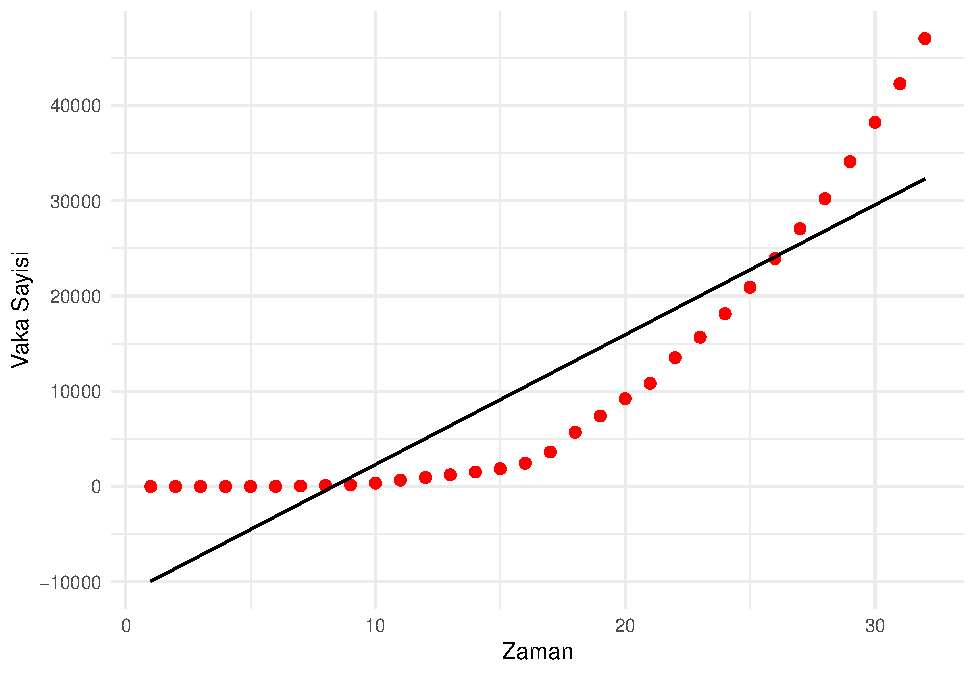
\includegraphics{rEkonometri_files/figure-latex/unnamed-chunk-41-1.pdf}

\begin{Shaded}
\begin{Highlighting}[]
\KeywordTok{summary}\NormalTok{(model_dogrusal)}
\end{Highlighting}
\end{Shaded}

\begin{verbatim}
## 
## Call:
## lm(formula = vaka ~ zaman, data = df)
## 
## Residuals:
##    Min     1Q Median     3Q    Max 
##  -8219  -5428  -1291   4853  14738 
## 
## Coefficients:
##             Estimate Std. Error t value Pr(>|t|)    
## (Intercept)   -11321       2382  -4.754 4.67e-05 ***
## zaman           1363        126  10.820 7.07e-12 ***
## ---
## Signif. codes:  0 '***' 0.001 '**' 0.01 '*' 0.05 '.' 0.1 ' ' 1
## 
## Residual standard error: 6579 on 30 degrees of freedom
## Multiple R-squared:  0.796,  Adjusted R-squared:  0.7892 
## F-statistic: 117.1 on 1 and 30 DF,  p-value: 7.073e-12
\end{verbatim}

Zamanın karesini aldığımız kuadratik model çıktısı:

\begin{Shaded}
\begin{Highlighting}[]
\KeywordTok{ggplot}\NormalTok{(df, }\KeywordTok{aes}\NormalTok{(}\DataTypeTok{x =}\NormalTok{ zaman)) }\OperatorTok{+}
\StringTok{  }\KeywordTok{geom_point}\NormalTok{(}\KeywordTok{aes}\NormalTok{(}\DataTypeTok{y =}\NormalTok{ vaka), }\DataTypeTok{color =} \StringTok{"red"}\NormalTok{, }\DataTypeTok{size =} \DecValTok{2}\NormalTok{) }\OperatorTok{+}
\StringTok{  }\KeywordTok{geom_line}\NormalTok{(}\KeywordTok{aes}\NormalTok{(}\DataTypeTok{y =}\NormalTok{ model_kuadratik}\OperatorTok{$}\NormalTok{fitted.values), }\DataTypeTok{color =} \StringTok{"black"}\NormalTok{) }\OperatorTok{+}
\StringTok{  }\KeywordTok{theme_minimal}\NormalTok{() }\OperatorTok{+}
\StringTok{  }\KeywordTok{labs}\NormalTok{(}\DataTypeTok{y =} \StringTok{"Vaka Sayısı"}\NormalTok{, }\DataTypeTok{x =} \StringTok{"Zaman"}\NormalTok{)}
\end{Highlighting}
\end{Shaded}

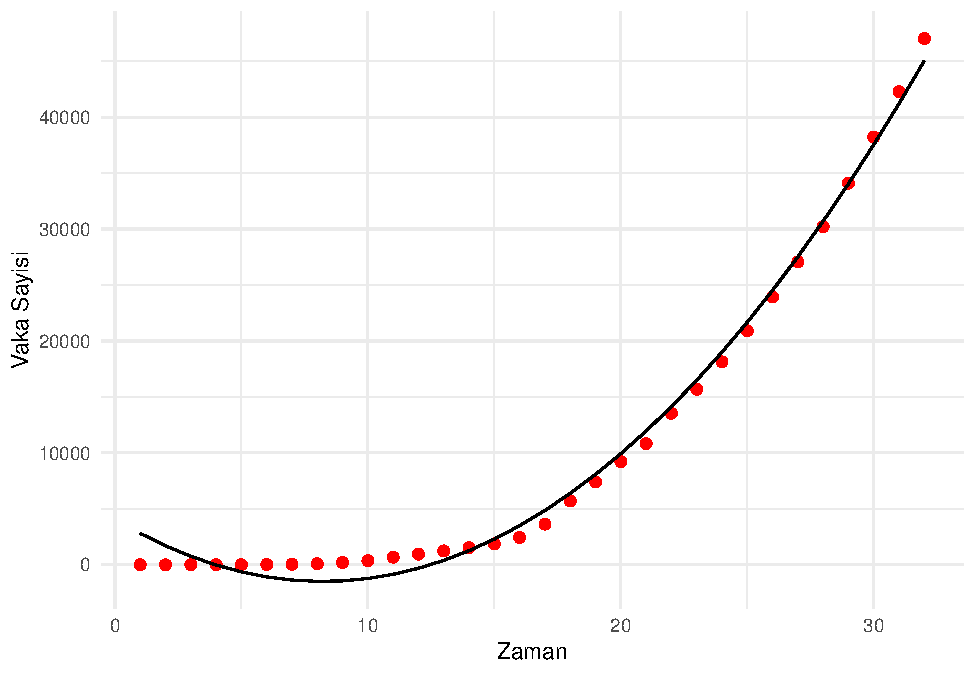
\includegraphics{rEkonometri_files/figure-latex/unnamed-chunk-42-1.pdf}

\begin{Shaded}
\begin{Highlighting}[]
\KeywordTok{summary}\NormalTok{(model_kuadratik)}
\end{Highlighting}
\end{Shaded}

\begin{verbatim}
## 
## Call:
## lm(formula = vaka ~ zaman + I(zaman^2), data = df)
## 
## Residuals:
##     Min      1Q  Median      3Q     Max 
## -2799.7  -750.3  -441.7  1074.0  1978.6 
## 
## Coefficients:
##              Estimate Std. Error t value Pr(>|t|)    
## (Intercept)  4071.917    675.913   6.024 1.49e-06 ***
## zaman       -1353.571     94.429 -14.334 1.08e-14 ***
## I(zaman^2)     82.317      2.776  29.652  < 2e-16 ***
## ---
## Signif. codes:  0 '***' 0.001 '**' 0.01 '*' 0.05 '.' 0.1 ' ' 1
## 
## Residual standard error: 1196 on 29 degrees of freedom
## Multiple R-squared:  0.9935, Adjusted R-squared:  0.993 
## F-statistic:  2212 on 2 and 29 DF,  p-value: < 2.2e-16
\end{verbatim}

Zamanın küpünü de aldığımız kübik model çıktısı:

\begin{Shaded}
\begin{Highlighting}[]
\KeywordTok{ggplot}\NormalTok{(df, }\KeywordTok{aes}\NormalTok{(}\DataTypeTok{x =}\NormalTok{ zaman)) }\OperatorTok{+}
\StringTok{  }\KeywordTok{geom_point}\NormalTok{(}\KeywordTok{aes}\NormalTok{(}\DataTypeTok{y =}\NormalTok{ vaka), }\DataTypeTok{color =} \StringTok{"red"}\NormalTok{, }\DataTypeTok{size =} \DecValTok{2}\NormalTok{) }\OperatorTok{+}
\StringTok{  }\KeywordTok{geom_line}\NormalTok{(}\KeywordTok{aes}\NormalTok{(}\DataTypeTok{y =}\NormalTok{ model_kubik}\OperatorTok{$}\NormalTok{fitted.values), }\DataTypeTok{color =} \StringTok{"black"}\NormalTok{) }\OperatorTok{+}
\StringTok{  }\KeywordTok{theme_minimal}\NormalTok{() }\OperatorTok{+}
\StringTok{  }\KeywordTok{labs}\NormalTok{(}\DataTypeTok{y =} \StringTok{"Vaka Sayısı"}\NormalTok{, }\DataTypeTok{x =} \StringTok{"Zaman"}\NormalTok{)}
\end{Highlighting}
\end{Shaded}

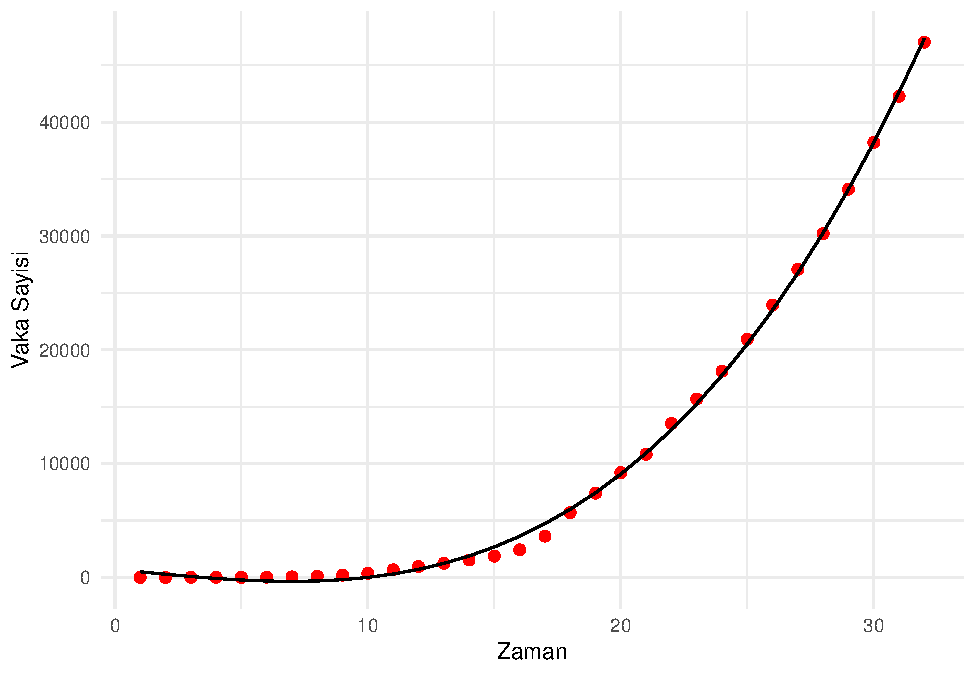
\includegraphics{rEkonometri_files/figure-latex/unnamed-chunk-43-1.pdf}

\begin{Shaded}
\begin{Highlighting}[]
\KeywordTok{summary}\NormalTok{(model_kubik)}
\end{Highlighting}
\end{Shaded}

\begin{verbatim}
## 
## Call:
## lm(formula = vaka ~ zaman + I(zaman^2) + I(zaman^3), data = df)
## 
## Residuals:
##      Min       1Q   Median       3Q      Max 
## -1185.71  -283.69    50.53   372.47   552.33 
## 
## Coefficients:
##              Estimate Std. Error t value Pr(>|t|)    
## (Intercept)  716.1536   372.9893   1.920   0.0651 .  
## zaman       -219.6015    96.3840  -2.278   0.0305 *  
## I(zaman^2)    -2.2819     6.7314  -0.339   0.7371    
## I(zaman^3)     1.7091     0.1342  12.734 3.63e-13 ***
## ---
## Signif. codes:  0 '***' 0.001 '**' 0.01 '*' 0.05 '.' 0.1 ' ' 1
## 
## Residual standard error: 466.9 on 28 degrees of freedom
## Multiple R-squared:  0.999,  Adjusted R-squared:  0.9989 
## F-statistic:  9723 on 3 and 28 DF,  p-value: < 2.2e-16
\end{verbatim}

Farklı farklı fonksiyon kalıplarını tanıdık. Peki, seçimi nasıl yapacağız? Gujarati, beceri ve deneyimin yanında şu maddelere de bakılabileceğini söylüyor:

\begin{enumerate}
\def\labelenumi{\roman{enumi}.}
\item
  Kuram, belli bir kalıbı önerebilir. Phillips eğrisi gibi.
\item
  Bağımlı değişkenin bağımsız değişkene göre eğimi hesaplanabileceği gibi esnekliği de hesaplanabilir.
\item
  Modelin parametreleri beklentileri karşılamalıdır. Araba talebinde fiyatın parametresini eksi beklemek gibi.
\item
  Bazen iki model de uygun düşebilir. Bu durumda \(R^2\) değerine bakılabilir. Fakat buna bakılırken iki modelde de bağımlı değişkenler aynı olmalıdır.
\item
  Bağımlı değişkenleri aynı olan iki model karşılaştırıldığında illa yüksek \(R^2\) değerini seçeceğiz gibi bir kural yoktur. Önemli olan kuramsal sağlamlık, tahmin edilen parametrelerin işaretleri, istatistiksel anlamlılıktır.
\item
  Bazen seçim yapmak kolay olmaz. Bu durumlarda Box-Cox dönüştürmeleri kullanılabilir.
\end{enumerate}

\emph{Uygun fonksiyon yapısını bulalım.}

wage değişkeninin dağılımını inceleyerek başlayalım.

\begin{Shaded}
\begin{Highlighting}[]
\NormalTok{df1 }\OperatorTok\StringTok{ }
\StringTok{  }\NormalTok{dplyr}\OperatorTok{::}\KeywordTok{select}\NormalTok{(wage, female, nonwhite, union, education, exper)}

\NormalTok{df1 }\OperatorTok\StringTok{ }
\StringTok{  }\KeywordTok{ggplot}\NormalTok{(}\KeywordTok{aes}\NormalTok{(}\DataTypeTok{x =}\NormalTok{ wage)) }\OperatorTok{+}
\StringTok{  }\KeywordTok{geom_histogram}\NormalTok{() }\OperatorTok{+}
\StringTok{  }\KeywordTok{theme_minimal}\NormalTok{()}
\end{Highlighting}
\end{Shaded}

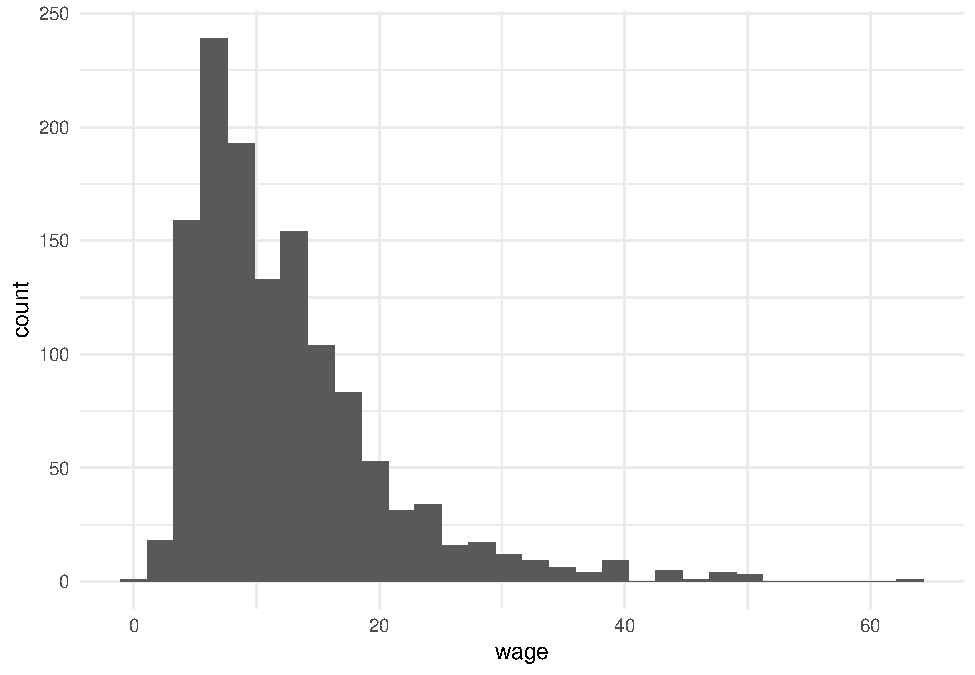
\includegraphics{rEkonometri_files/figure-latex/unnamed-chunk-44-1.pdf}

Dağılım çarpık eğilim göstermektedir. Diğer bir ifadeyle dağılım sağa çarpıktır ve normal dağılımdan uzaktır. Bir değişkenin normal dağılıma sahip olması için skewness denilen çarpıklık parametresinin (simetrinin bir ölçüsü) 0, kurtosis denilen basıklık parametresinin (diklik veya yatıklığın bir ölçüsü) 3 olması gerekmektedir.

\begin{Shaded}
\begin{Highlighting}[]
\KeywordTok{skewness}\NormalTok{(df1}\OperatorTok{$}\NormalTok{wage)}
\end{Highlighting}
\end{Shaded}

\begin{verbatim}
## [1] 1.848114
\end{verbatim}

\begin{Shaded}
\begin{Highlighting}[]
\KeywordTok{kurtosis}\NormalTok{(df1}\OperatorTok{$}\NormalTok{wage)}
\end{Highlighting}
\end{Shaded}

\begin{verbatim}
## [1] 7.836566
\end{verbatim}

Bulduğumuz her iki değer de belirttiğimiz değerlerden farklıdır. Skewness ve kurtosis ölçülerine dayanan Jarque-Bera (J-B) istatistik ve buna ait p değeri aşağıdaki gibidir:

\begin{Shaded}
\begin{Highlighting}[]
\KeywordTok{jarque.test}\NormalTok{(df1}\OperatorTok{$}\NormalTok{wage)}
\end{Highlighting}
\end{Shaded}

\begin{verbatim}
## 
##  Jarque-Bera Normality Test
## 
## data:  df1$wage
## JB = 1990.1, p-value < 2.2e-16
## alternative hypothesis: greater
\end{verbatim}

Normal dağılmış bir değişken için skewness = 0, kurtosis = 3'tür demiştik. Dolayısıyla, J-B testi skewness ile kurtosis'in sırasıyla 0 ve 3 olduğu bir bileşik hipotez testidir. Bu durumda J-B istatistiğinin sıfır olması beklenir. Eğer \(\chi^2\) istatistiğinin p değeri yeterince düşükse, ki bu durum J-B istatistiği 0'dan çok farklı ise ortaya çıkar, normal dağılım varsayımını ileri süren \(H_0\) reddedilebilir. Ama p değeri yüksekse, ki bu durum J-B istatistiği sıfıra yakınsa ortaya çıkar, normallik varsayımı reddedilemez. Uygulamamızda, J-B değeri sıfırdan çok uzaktır ve böyle bir değer elde etmenin olasılığı (p değeri) neredeyse sıfırdır. Yani, normal dağılım varsayımını ileri süren \(H_0\)'ı reddettik.

Peki, wage'in logaritmasını alsaydık nasıl olurdu?

\begin{Shaded}
\begin{Highlighting}[]
\NormalTok{df1 }\OperatorTok\StringTok{ }
\StringTok{  }\KeywordTok{mutate}\NormalTok{(}\DataTypeTok{lnwage =} \KeywordTok{log}\NormalTok{(wage))}

\NormalTok{df1 }\OperatorTok\StringTok{ }
\StringTok{  }\KeywordTok{ggplot}\NormalTok{(}\KeywordTok{aes}\NormalTok{(}\DataTypeTok{x =}\NormalTok{ lnwage)) }\OperatorTok{+}
\StringTok{  }\KeywordTok{geom_histogram}\NormalTok{() }\OperatorTok{+}
\StringTok{  }\KeywordTok{theme_minimal}\NormalTok{()}
\end{Highlighting}
\end{Shaded}

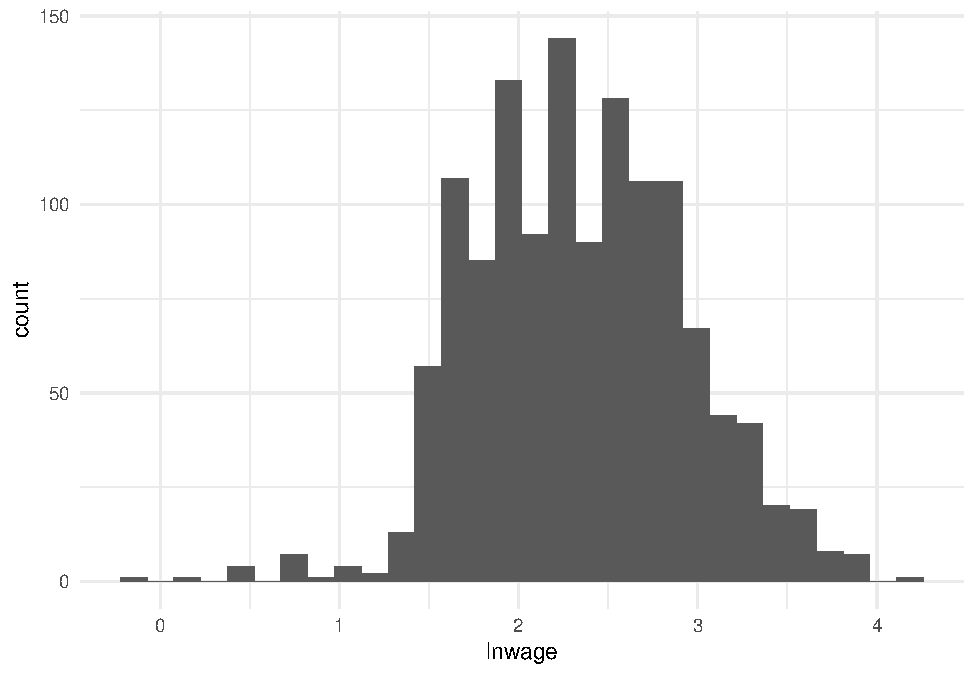
\includegraphics{rEkonometri_files/figure-latex/unnamed-chunk-47-1.pdf}

\begin{Shaded}
\begin{Highlighting}[]
\KeywordTok{skewness}\NormalTok{(df1}\OperatorTok{$}\NormalTok{lnwage)}
\end{Highlighting}
\end{Shaded}

\begin{verbatim}
## [1] 0.01339502
\end{verbatim}

\begin{Shaded}
\begin{Highlighting}[]
\KeywordTok{kurtosis}\NormalTok{(df1}\OperatorTok{$}\NormalTok{lnwage)}
\end{Highlighting}
\end{Shaded}

\begin{verbatim}
## [1] 3.226337
\end{verbatim}

\begin{Shaded}
\begin{Highlighting}[]
\KeywordTok{jarque.test}\NormalTok{(df1}\OperatorTok{$}\NormalTok{lnwage)}
\end{Highlighting}
\end{Shaded}

\begin{verbatim}
## 
##  Jarque-Bera Normality Test
## 
## data:  df1$lnwage
## JB = 2.7899, p-value = 0.2478
## alternative hypothesis: greater
\end{verbatim}

Logaritması alınmış wage ile normal dağılıma ulaşmış olduk. Bunu kullanarak modeli oluşturalım.

\begin{Shaded}
\begin{Highlighting}[]
\NormalTok{model <-}\StringTok{ }\KeywordTok{lm}\NormalTok{(}\DataTypeTok{formula =}\NormalTok{ lnwage }\OperatorTok{~}\StringTok{ }\NormalTok{female }\OperatorTok{+}\StringTok{ }\NormalTok{nonwhite }\OperatorTok{+}\StringTok{ }\NormalTok{union }\OperatorTok{+}\StringTok{ }\NormalTok{education }\OperatorTok{+}\StringTok{ }\NormalTok{exper, }\DataTypeTok{data =}\NormalTok{ df1)}
\KeywordTok{summary}\NormalTok{(model)}
\end{Highlighting}
\end{Shaded}

\begin{verbatim}
## 
## Call:
## lm(formula = lnwage ~ female + nonwhite + union + education + 
##     exper, data = df1)
## 
## Residuals:
##      Min       1Q   Median       3Q      Max 
## -2.51287 -0.28288  0.00345  0.30683  1.79761 
## 
## Coefficients:
##              Estimate Std. Error t value Pr(>|t|)    
## (Intercept)  0.905504   0.074175  12.208  < 2e-16 ***
## female      -0.249154   0.026625  -9.358  < 2e-16 ***
## nonwhite    -0.133535   0.037182  -3.591 0.000341 ***
## union        0.180204   0.036955   4.876 1.22e-06 ***
## education    0.099870   0.004812  20.752  < 2e-16 ***
## exper        0.012760   0.001172  10.889  < 2e-16 ***
## ---
## Signif. codes:  0 '***' 0.001 '**' 0.01 '*' 0.05 '.' 0.1 ' ' 1
## 
## Residual standard error: 0.4752 on 1283 degrees of freedom
## Multiple R-squared:  0.3457, Adjusted R-squared:  0.3431 
## F-statistic: 135.5 on 5 and 1283 DF,  p-value: < 2.2e-16
\end{verbatim}

Parametreler hem t testine göre hem de F testine göre anlamlıdır.

Bu modelde wage değişkeni logaritmik; bağımsız değişkenler ise doğrusal yapıdadır. Yani, yarı logaritmiktir.

Diğer tüm değişkenler sabit tutulduğunda;

Her ilave eğitim yılı için ortalama wage oranının 100*0.099 = \%9.99 artacağını söyleyebiliriz (education).

Her ilave yıllık iş deneyimi için ortalama wage oranının 100*0.013 = \%1.3 artacağını söyleyebiliriz (exper).

Ortalama kadın wage oranı ortalama erkek wage oranına göre \%24.92 daha düşüktür (female). Ancak biz doğru olan yüzdeyi parametrenin ters logaritmasını alıp 1'den çıkararak buluyorduk.

\begin{Shaded}
\begin{Highlighting}[]
\KeywordTok{exp}\NormalTok{(}\KeywordTok{as.numeric}\NormalTok{(model}\OperatorTok{$}\NormalTok{coefficients[}\DecValTok{2}\NormalTok{])) }\OperatorTok{-}\StringTok{ }\DecValTok{1}
\end{Highlighting}
\end{Shaded}

\begin{verbatim}
## [1] -0.2205401
\end{verbatim}

Kadın ortalama wage oranı erkek ortalama wage oranından \%22.06 daha düşüktür. Bu da \%24.92'den farklıdır. Çıktıdaki parametreler yaklaşık değişimi verirken ikinci yöntem kesin değişimi verir.

Beyaz olmayan işçinin ortalama wage oranı beyaz olan işçinin ortalama wage oranından \%12.5 daha düşüktür (nonwhite).

\begin{Shaded}
\begin{Highlighting}[]
\KeywordTok{exp}\NormalTok{(}\KeywordTok{as.numeric}\NormalTok{(model}\OperatorTok{$}\NormalTok{coefficients[}\DecValTok{3}\NormalTok{])) }\OperatorTok{-}\StringTok{ }\DecValTok{1}
\end{Highlighting}
\end{Shaded}

\begin{verbatim}
## [1] -0.1250032
\end{verbatim}

Sendikalı işçinin ortalama wage oranı sendikasız işçinin ortalama wage oranından \%19.75 daha fazladır (union).

\begin{Shaded}
\begin{Highlighting}[]
\KeywordTok{exp}\NormalTok{(}\KeywordTok{as.numeric}\NormalTok{(model}\OperatorTok{$}\NormalTok{coefficients[}\DecValTok{4}\NormalTok{])) }\OperatorTok{-}\StringTok{ }\DecValTok{1}
\end{Highlighting}
\end{Shaded}

\begin{verbatim}
## [1] 0.1974611
\end{verbatim}

Aşağıdaki çıktıyı hatırlayalım (wage değişkeni logaritmasız):

\begin{Shaded}
\begin{Highlighting}[]
\NormalTok{model <-}\StringTok{ }\KeywordTok{lm}\NormalTok{(}\DataTypeTok{formula =}\NormalTok{ wage }\OperatorTok{~}\StringTok{ }\NormalTok{female }\OperatorTok{+}\StringTok{ }\NormalTok{nonwhite }\OperatorTok{+}\StringTok{ }\NormalTok{union }\OperatorTok{+}\StringTok{ }\NormalTok{education }\OperatorTok{+}\StringTok{ }\NormalTok{exper, }\DataTypeTok{data =}\NormalTok{ df1)}
\KeywordTok{summary}\NormalTok{(model)}
\end{Highlighting}
\end{Shaded}

\begin{verbatim}
## 
## Call:
## lm(formula = wage ~ female + nonwhite + union + education + exper, 
##     data = df1)
## 
## Residuals:
##     Min      1Q  Median      3Q     Max 
## -20.781  -3.760  -1.044   2.418  50.414 
## 
## Coefficients:
##             Estimate Std. Error t value Pr(>|t|)    
## (Intercept) -7.18334    1.01579  -7.072 2.51e-12 ***
## female      -3.07488    0.36462  -8.433  < 2e-16 ***
## nonwhite    -1.56531    0.50919  -3.074  0.00216 ** 
## union        1.09598    0.50608   2.166  0.03052 *  
## education    1.37030    0.06590  20.792  < 2e-16 ***
## exper        0.16661    0.01605  10.382  < 2e-16 ***
## ---
## Signif. codes:  0 '***' 0.001 '**' 0.01 '*' 0.05 '.' 0.1 ' ' 1
## 
## Residual standard error: 6.508 on 1283 degrees of freedom
## Multiple R-squared:  0.3233, Adjusted R-squared:  0.3207 
## F-statistic: 122.6 on 5 and 1283 DF,  p-value: < 2.2e-16
\end{verbatim}

wage'i logaritmasız olan model ile wage'i logaritmalı modelin \(R^2\) değerlerini karşılaştırarak karar verebilir miyiz?

Baktığımız zaman wage'i logaritmasız olan model de parametreler açısından anlamlıdır.

Hatırlayalım:

\begin{quote}
\emph{Bazen iki model de uygun düşebilir. Bu durumda} \(R^2\) \emph{değerine bakılabilir. Fakat buna bakılırken iki modelde de bağımlı değişkenler aynı olmalıdır.}
\end{quote}

Yani, \(R^2\) doğrusal modelde bağımlı değişkendeki değişkenliğin bütün bağımsız değişkenlerce açıklanan oranını ölçerken, yarı-logaritmik modelde bağımlı değişkenin logaritmasındaki değişkenliğin oranını ölçer. Bu ikisi aynı şey değildir.

\hypertarget{kukla-deux11fiux15fkenli-regresyon-modeli}{%
\chapter{Kukla Değişkenli Regresyon Modeli}\label{kukla-deux11fiux15fkenli-regresyon-modeli}}

\hypertarget{kukla-deux11fiux15fkenlerin-yorumu}{%
\section{Kukla Değişkenlerin Yorumu}\label{kukla-deux11fiux15fkenlerin-yorumu}}

Kukla değişken derken aynı zamanda nitel değişkenlerden bahsediyoruz. Nitel değişkenlerin belirli bir sayısal değeri yoktur. Yani, nominal ölçek değişkenlerdir. Ama biz 0 ve 1 değerleri ile sayısallaştırıp kukla değişkenler oluşturuyoruz.

Üç tane kukla değişkenimiz vardı: female (kadın ise 1; değilse 0), nonwhite (beyaz olmayan işçi ise 1; değilse 0), union (sendikalı bir iş ise 1; değilse 0).

Kukla değişkeni D (dummy) ile ifade edelim. wage fonksiyonunu şöyle yazabiliriz:

\(wage_i = \beta_1 + \beta_2D_{2i} + \beta_3D_{3i} + \beta_4D_{4i} + \beta_5education_i + \beta_6exper_i + \epsilon_i\)

\(D_{2i}: kadın = 1; erkek = 0\)

\(D_{3i}: beyaz değil = 1; beyaz = 0\)

\(D_{4i}: sendikalı = 1; sendikasız = 0\)

\begin{Shaded}
\begin{Highlighting}[]
\KeywordTok{library}\NormalTok{(readxl);}\KeywordTok{library}\NormalTok{(tidyverse);}\KeywordTok{library}\NormalTok{(magrittr);}\KeywordTok{library}\NormalTok{(segmented)}

\KeywordTok{setwd}\NormalTok{(}\StringTok{"C:/Users/datanerd/Desktop/Github/rEkonometri/data"}\NormalTok{)}
\NormalTok{df1 <-}\StringTok{ }\KeywordTok{read_excel}\NormalTok{(}\StringTok{"Table1_1.xls"}\NormalTok{)}
\NormalTok{df2 <-}\StringTok{ }\KeywordTok{read_excel}\NormalTok{(}\StringTok{"Table3_6.xls"}\NormalTok{)}
\NormalTok{df3 <-}\StringTok{ }\KeywordTok{read_excel}\NormalTok{(}\StringTok{"Table3_10.xls"}\NormalTok{)}
\end{Highlighting}
\end{Shaded}

\begin{Shaded}
\begin{Highlighting}[]
\NormalTok{df1 }\OperatorTok\StringTok{ }
\StringTok{  }\NormalTok{dplyr}\OperatorTok{::}\KeywordTok{select}\NormalTok{(wage, female, nonwhite, union, education, exper)}

\NormalTok{model <-}\StringTok{ }\KeywordTok{lm}\NormalTok{(}\DataTypeTok{formula =}\NormalTok{ wage }\OperatorTok{~}\StringTok{ }\NormalTok{female }\OperatorTok{+}\StringTok{ }\NormalTok{nonwhite }\OperatorTok{+}\StringTok{ }\NormalTok{union }\OperatorTok{+}\StringTok{ }\NormalTok{education }\OperatorTok{+}\StringTok{ }\NormalTok{exper, }\DataTypeTok{data =}\NormalTok{ df1)}
\KeywordTok{summary}\NormalTok{(model)}
\end{Highlighting}
\end{Shaded}

\begin{verbatim}
## 
## Call:
## lm(formula = wage ~ female + nonwhite + union + education + exper, 
##     data = df1)
## 
## Residuals:
##     Min      1Q  Median      3Q     Max 
## -20.781  -3.760  -1.044   2.418  50.414 
## 
## Coefficients:
##             Estimate Std. Error t value Pr(>|t|)    
## (Intercept) -7.18334    1.01579  -7.072 2.51e-12 ***
## female      -3.07488    0.36462  -8.433  < 2e-16 ***
## nonwhite    -1.56531    0.50919  -3.074  0.00216 ** 
## union        1.09598    0.50608   2.166  0.03052 *  
## education    1.37030    0.06590  20.792  < 2e-16 ***
## exper        0.16661    0.01605  10.382  < 2e-16 ***
## ---
## Signif. codes:  0 '***' 0.001 '**' 0.01 '*' 0.05 '.' 0.1 ' ' 1
## 
## Residual standard error: 6.508 on 1283 degrees of freedom
## Multiple R-squared:  0.3233, Adjusted R-squared:  0.3207 
## F-statistic: 122.6 on 5 and 1283 DF,  p-value: < 2.2e-16
\end{verbatim}

\begin{itemize}
\item
  Eğer modele kesme terimi dahil ettiysek ve bir nitel değişkenin m sayıda kategorisi varsa bu durumda m-1 adet kukla değişken belirleriz. Örnek olarak nonwhite değişkenine bakalım. Eğer işçi beyaz değilse 1 olarak kodladık. Zorunlu olarak beyaz olanları da 0 olarak kodlamalıyız. Bu durumda nonwhite'ın iki kategorisi olduğu için 1 tane kukla değişken belirleriz. Burada hangisine 0-1 verildiğinin bir önemi yoktur. Peki, kategorisi ikiden fazla olan bir nitel değişken olsaydı? Örneğin, 3 tane. Bu durumda en fazla iki (3-1) kukla değişkenimiz olabilir. Bu kuralı izlemezsek kukla değişken tuzağına yakalanırız. Yani, tam doğrusal bağlantı durumu. Eğer üç kategori için üç kukla değişkenimiz ve bir de kesme terimimiz varsa bu üç kukla değişkenin toplamı 1 olup bu da 1 olan kesme terimine eşit olacaktır. İşte tam doğrusallık. female örneğine bakalım. Bu örnekte kadınlar için 1; erkekler için 0 idi. Erkekler için 1; kadınlar için 0 değerini alan erkek kukla değişkenini de modele neden dahil etmiyoruz diye sorabiliriz. Bu gereksizdir. Çünkü, erkekler için kesme terimi \(\beta_1\); kadınlar için kesme terimi \(\beta_1 + \beta_2\)'dir. Sadece iki kategori olduğu için sadece iki farklı kesme terimine ihtiyacımız vardır. Bu da şu anlama gelir: \(\beta_1\)'in yanı sıra sadece bir tane kukla değişken kullanmamız gerekir. Biz de ilk başta kadınlar için bir kukla değişken kullanmayı tercih ettik.
\item
  Eğer bir nitel değişkenin m kategorisi varsa, kesme terimi dahil etmemek koşuluyla m adet kukla değişken ekleyebiliriz.
\item
  0 değerini alan kategori referanstır. Tüm karşılaştırmalar bu referansa göre yapılır.
\item
  Kukla değişkenler logaritmik yapıda belirlenemez. Çünkü, 0-1 olarak belirleniyorlar.
\item
  Her kukla parametresi bir serbestlik derecesine mal olur. Bu nedenle küçük örneklemlerde fazla kukla parametresi belirlemekten kaçınmalıyız.
\end{itemize}

Kukla değişkenler ile ilgili yorumları vermiştik. Diğer değişkenler sabit tutulduğunda;

Kuklaların yorumu:

Kadınların ortalama wage'i erkeklerin ortalama wage'inden 3.08 \$ daha düşüktür (female).

Beyaz olmayan bir işçinin ortalama wage'i beyaz bir işçinin ortalama wage'inden 1.57 \$ daha düşüktür (nonwhite).

Sendikalı bir işte çalışanın ortalama wage'i sendikalı bir işte çalışmayanın ortalama wage'inden 1.1 \$ daha fazladır (union).

Kukla olmayanların yorumu:

Her ilave eğitim yılı için ortalama wage 1.37 \$ artmaktadır (education).

Her ilave deneyim için ortalama wage 0.17 \$ artmaktadır (exper).

Örneğin, female için ne dedik? Kadınların ortalama wage'i erkeklerin ortalama wage'inden\ldots{} Burada erkeklere sıfır dediğimiz için referans erkek kategorisi oldu.

-7.18334 olan kesme terimi ise sıfır değeri alan tüm kategorileri işaret etmektedir. Yani, erkek, beyaz, sendikalı olmayan işçilerin beklenen ücreti. Ücret eksi çıkar mı? Yorumlarken tabi ki dikkat edeceğiz. Bunun iktisadi açıdan bir anlamı yoktur.

Bir kadın işçinin erkek işçiye göre ortalama wage'inin ne kadar düşük olduğunu biliyoruz. Ya da beyaz olmayan bir işçinin beyaz işçiye göre\ldots{} Ya da sendika üyesi bir işçinin sendika üyesi olmayan bir işçiye göre\ldots{} Peki, beyaz olmayan bir kadın işçinin ortalama wage'inin, sadece kadın bir işçinin veya sadece beyaz olmayan bir işçinin ortalama wage'inden farklı olması mümkün müdür?

Bunu belirlemek için kadın ve beyaz olmayan kuklaların çarpımını wage fonksiyonuna ekleriz. Bu tür çarpıma etkileşimli kukla diyeceğiz.

\begin{Shaded}
\begin{Highlighting}[]
\NormalTok{df1 }\OperatorTok\StringTok{ }
\StringTok{  }\KeywordTok{mutate}\NormalTok{(}\DataTypeTok{female_nonwhite =}\NormalTok{ female }\OperatorTok{*}\StringTok{ }\NormalTok{nonwhite)}

\NormalTok{model <-}\StringTok{ }\KeywordTok{lm}\NormalTok{(}\DataTypeTok{formula =}\NormalTok{ wage }\OperatorTok{~}\StringTok{ }\NormalTok{female }\OperatorTok{+}\StringTok{ }\NormalTok{nonwhite }\OperatorTok{+}\StringTok{ }\NormalTok{union }\OperatorTok{+}\StringTok{ }\NormalTok{education }\OperatorTok{+}\StringTok{ }\NormalTok{exper }\OperatorTok{+}\StringTok{ }\NormalTok{female_nonwhite, }\DataTypeTok{data =}\NormalTok{ df1)}
\KeywordTok{summary}\NormalTok{(model)}
\end{Highlighting}
\end{Shaded}

\begin{verbatim}
## 
## Call:
## lm(formula = wage ~ female + nonwhite + union + education + exper + 
##     female_nonwhite, data = df1)
## 
## Residuals:
##     Min      1Q  Median      3Q     Max 
## -20.844  -3.746  -1.016   2.452  50.497 
## 
## Coefficients:
##                 Estimate Std. Error t value Pr(>|t|)    
## (Intercept)     -7.08873    1.01948  -6.953 5.67e-12 ***
## female          -3.24015    0.39533  -8.196 5.96e-16 ***
## nonwhite        -2.15853    0.74843  -2.884  0.00399 ** 
## union            1.11504    0.50635   2.202  0.02783 *  
## education        1.37011    0.06590  20.791  < 2e-16 ***
## exper            0.16586    0.01606  10.326  < 2e-16 ***
## female_nonwhite  1.09537    1.01290   1.081  0.27971    
## ---
## Signif. codes:  0 '***' 0.001 '**' 0.01 '*' 0.05 '.' 0.1 ' ' 1
## 
## Residual standard error: 6.508 on 1282 degrees of freedom
## Multiple R-squared:  0.324,  Adjusted R-squared:  0.3208 
## F-statistic: 102.4 on 6 and 1282 DF,  p-value: < 2.2e-16
\end{verbatim}

Diğer faktörler sabit tutulduğunda, kadın olmanın 3.24 \$ daha düşük ortalama wage'i vardır. Beyaz olmamanın ortalama 2.16 \$ daha düşük ortalama wage'i vardır. Hem kadın hem de beyaz olmamanın ise female + nonwhite + female\_nonwhite = -- 3.24 -- 2.16 + 1.10 = -4.30 \$ daha düşük ortalama wage'i vardır. Başka bir ifade ile, beyaz olmayan bir kadın sadece kadın olmaktan veya sadece beyaz olmamaktan daha düşük bir ortalama wage elde eder.

Kukla değişken olmayan örneğin, education için şu yorumu yapmıştık: Her ilave eğitim yılı için ortalama wage 1.37 \$ artmaktadır. Bunu derken aslında kadın ile erkek arasında, beyaz olmayan ile beyaz arasında ve sendikalı ile sendikasız arasında aynı olduğunu kabul ediyoruz.

Ücret fonksiyonunu şöyle ifade edelim:

\(wage_i = \beta_1 + \beta_2D_{2i} + \beta_3D_{3i} + \beta_4D_{4i} + \beta_5education_i + \beta_6exper_i + \beta_7(D_{2i}*education_i) +\)

\(\beta_8(D_{3i}*education_i) + \beta_9(D_{4i}*education_i) + \beta_{10}(D_{2i}*exper_i) + \beta_{11}(D_{3i}*exper_i) +\)

\(\beta_{12}(D_{4i}*exper_i) + \epsilon_i\)

\(\beta_2, \beta_3, \beta_4\)'ü yazmıştık; önceden biliyoruz. \(\beta_7\) ile \(\beta_{11}\) arasını ise aşağıdaki gibi yorumlayacağız.

\begin{Shaded}
\begin{Highlighting}[]
\NormalTok{df1 }\OperatorTok\StringTok{ }
\StringTok{  }\KeywordTok{mutate}\NormalTok{(}\DataTypeTok{female_educ =}\NormalTok{ female }\OperatorTok{*}\StringTok{ }\NormalTok{education,}
         \DataTypeTok{nonwhite_educ =}\NormalTok{ nonwhite }\OperatorTok{*}\StringTok{ }\NormalTok{education,}
         \DataTypeTok{union_educ =}\NormalTok{ union }\OperatorTok{*}\StringTok{ }\NormalTok{education,}
         \DataTypeTok{female_exper =}\NormalTok{ female }\OperatorTok{*}\StringTok{ }\NormalTok{exper,}
         \DataTypeTok{nonwhite_exper =}\NormalTok{ nonwhite }\OperatorTok{*}\StringTok{ }\NormalTok{exper,}
         \DataTypeTok{union_exper =}\NormalTok{ union }\OperatorTok{*}\StringTok{ }\NormalTok{exper)}

\NormalTok{model <-}\StringTok{ }\KeywordTok{lm}\NormalTok{(}\DataTypeTok{formula =}\NormalTok{ wage }\OperatorTok{~}\StringTok{ }\NormalTok{female }\OperatorTok{+}\StringTok{ }\NormalTok{nonwhite }\OperatorTok{+}\StringTok{ }\NormalTok{union }\OperatorTok{+}\StringTok{ }\NormalTok{education }\OperatorTok{+}\StringTok{ }\NormalTok{exper }\OperatorTok{+}\StringTok{ }\NormalTok{female_educ }\OperatorTok{+}\StringTok{ }\NormalTok{nonwhite_educ }\OperatorTok{+}\StringTok{ }\NormalTok{union_educ }\OperatorTok{+}\StringTok{ }\NormalTok{female_exper }\OperatorTok{+}\StringTok{ }\NormalTok{nonwhite_exper }\OperatorTok{+}\StringTok{ }\NormalTok{union_exper, }\DataTypeTok{data =}\NormalTok{ df1)}
\KeywordTok{summary}\NormalTok{(model)}
\end{Highlighting}
\end{Shaded}

\begin{verbatim}
## 
## Call:
## lm(formula = wage ~ female + nonwhite + union + education + exper + 
##     female_educ + nonwhite_educ + union_educ + female_exper + 
##     nonwhite_exper + union_exper, data = df1)
## 
## Residuals:
##     Min      1Q  Median      3Q     Max 
## -23.164  -3.570  -1.070   2.337  50.496 
## 
## Coefficients:
##                 Estimate Std. Error t value Pr(>|t|)    
## (Intercept)    -11.09129    1.42185  -7.801 1.27e-14 ***
## female           3.17416    1.96646   1.614  0.10674    
## nonwhite         2.90913    2.78007   1.046  0.29556    
## union            4.45421    2.97349   1.498  0.13439    
## education        1.58712    0.09382  16.917  < 2e-16 ***
## exper            0.22091    0.02511   8.799  < 2e-16 ***
## female_educ     -0.33689    0.13199  -2.552  0.01082 *  
## nonwhite_educ   -0.32186    0.19535  -1.648  0.09968 .  
## union_educ      -0.19832    0.19137  -1.036  0.30025    
## female_exper    -0.09612    0.03181  -3.022  0.00257 ** 
## nonwhite_exper  -0.02204    0.04438  -0.497  0.61949    
## union_exper     -0.03345    0.04605  -0.726  0.46772    
## ---
## Signif. codes:  0 '***' 0.001 '**' 0.01 '*' 0.05 '.' 0.1 ' ' 1
## 
## Residual standard error: 6.478 on 1277 degrees of freedom
## Multiple R-squared:  0.3328, Adjusted R-squared:  0.3271 
## F-statistic: 57.91 on 11 and 1277 DF,  p-value: < 2.2e-16
\end{verbatim}

female\_educ ve female\_exper parametreleri negatif ve istatistiksel olarak anlamlıdır. Bu da education ve exper'e göre kadın işçiler için ortalama saatlik wage artış hızı, erkek işçilere göre daha düşük demektir. Aynı şekilde nonwhite\_educ için yorum education'a göre wage artış hızı beyaz olmayan işçiler için negatiftir; beyaz işçilerinkinden daha düşüktür. Bu parametre \%10 seviyesinde istatistiksel olarak anlamlıdır. Diğer parametreler istatistiksel olarak anlamlı değildir. Bunları modelden çıkartıp modeli yeniden kuralım.

\begin{Shaded}
\begin{Highlighting}[]
\NormalTok{model <-}\StringTok{ }\KeywordTok{lm}\NormalTok{(}\DataTypeTok{formula =}\NormalTok{ wage }\OperatorTok{~}\StringTok{ }\NormalTok{female }\OperatorTok{+}\StringTok{ }\NormalTok{nonwhite }\OperatorTok{+}\StringTok{ }\NormalTok{union }\OperatorTok{+}\StringTok{ }\NormalTok{education }\OperatorTok{+}\StringTok{ }\NormalTok{exper }\OperatorTok{+}\StringTok{ }\NormalTok{female_educ }\OperatorTok{+}\StringTok{ }\NormalTok{nonwhite_educ }\OperatorTok{+}\StringTok{ }\NormalTok{female_exper, }\DataTypeTok{data =}\NormalTok{ df1)}
\KeywordTok{summary}\NormalTok{(model)}
\end{Highlighting}
\end{Shaded}

\begin{verbatim}
## 
## Call:
## lm(formula = wage ~ female + nonwhite + union + education + exper + 
##     female_educ + nonwhite_educ + female_exper, data = df1)
## 
## Residuals:
##     Min      1Q  Median      3Q     Max 
## -22.885  -3.552  -1.109   2.389  50.553 
## 
## Coefficients:
##                Estimate Std. Error t value Pr(>|t|)    
## (Intercept)   -10.64520    1.37180  -7.760 1.73e-14 ***
## female          3.25747    1.95925   1.663  0.09664 .  
## nonwhite        2.62695    2.41787   1.086  0.27747    
## union           1.07851    0.50540   2.134  0.03303 *  
## education       1.56580    0.09181  17.054  < 2e-16 ***
## exper           0.21262    0.02277   9.338  < 2e-16 ***
## female_educ    -0.34695    0.13149  -2.639  0.00842 ** 
## nonwhite_educ  -0.32937    0.18663  -1.765  0.07783 .  
## female_exper   -0.09491    0.03156  -3.007  0.00269 ** 
## ---
## Signif. codes:  0 '***' 0.001 '**' 0.01 '*' 0.05 '.' 0.1 ' ' 1
## 
## Residual standard error: 6.474 on 1280 degrees of freedom
## Multiple R-squared:  0.332,  Adjusted R-squared:  0.3278 
## F-statistic: 79.52 on 8 and 1280 DF,  p-value: < 2.2e-16
\end{verbatim}

Kategorinin 0 ve 1 olmasına göre aldığımız aksiyonlara dikkat edin.

Beyaz, erkek, sendikalı olmayan işçilerin (hepsi sıfırı temsil ediyor) ücret fonksiyonu:

\(\hat{wage_i} = -10.6452 + 1.5658education_i + 0.21262exper_i\)

Beyaz, kadın, sendikalı olmayan işçilerin ücret fonksiyonu:

\(\hat{wage_i} = (-10.6452 + 3.2574) + (1.5658 – 0.34695)education_i + (0.21262 – 0.0949)exper_i\)

\(\hat{wage_i} = -7.3878 + 1.21885education_i + 0.11772exper_i\)

Beyaz olmayan, erkek, sendikalı olmayan işçilerin ücret fonksiyonu:

\(\hat{wage_i} = (-10.6452 + 2.62695) + (1.5658 – 0.32937)education_i + 0.21262exper_i\)

\(\hat{wage_i} = -8.01825 + 1.23643education_i + 0.21262exper_i\)

Beyaz, erkek, sendikalı işçilerin ücret fonksiyonu:

\(\hat{wage_i} = (-10.6452 + 1.07851) + 1.5658education_i + 0.21262exper_i\)

\(\hat{wage_i} = -9.56669 + 1.5658education_i + 0.21262exper_i\)

Bağımlı değişken logaritmik olsaydı kukla değişkenleri nasıl yorumlayacaktık?

\begin{Shaded}
\begin{Highlighting}[]
\NormalTok{df1 }\OperatorTok\StringTok{ }
\StringTok{  }\KeywordTok{mutate}\NormalTok{(}\DataTypeTok{lnwage =} \KeywordTok{log}\NormalTok{(wage))}

\NormalTok{model <-}\StringTok{ }\KeywordTok{lm}\NormalTok{(}\DataTypeTok{formula =}\NormalTok{ lnwage }\OperatorTok{~}\StringTok{ }\NormalTok{female }\OperatorTok{+}\StringTok{ }\NormalTok{nonwhite }\OperatorTok{+}\StringTok{ }\NormalTok{union }\OperatorTok{+}\StringTok{ }\NormalTok{education }\OperatorTok{+}\StringTok{ }\NormalTok{exper, }\DataTypeTok{data =}\NormalTok{ df1)}
\KeywordTok{summary}\NormalTok{(model)}
\end{Highlighting}
\end{Shaded}

\begin{verbatim}
## 
## Call:
## lm(formula = lnwage ~ female + nonwhite + union + education + 
##     exper, data = df1)
## 
## Residuals:
##      Min       1Q   Median       3Q      Max 
## -2.51287 -0.28288  0.00345  0.30683  1.79761 
## 
## Coefficients:
##              Estimate Std. Error t value Pr(>|t|)    
## (Intercept)  0.905504   0.074175  12.208  < 2e-16 ***
## female      -0.249154   0.026625  -9.358  < 2e-16 ***
## nonwhite    -0.133535   0.037182  -3.591 0.000341 ***
## union        0.180204   0.036955   4.876 1.22e-06 ***
## education    0.099870   0.004812  20.752  < 2e-16 ***
## exper        0.012760   0.001172  10.889  < 2e-16 ***
## ---
## Signif. codes:  0 '***' 0.001 '**' 0.01 '*' 0.05 '.' 0.1 ' ' 1
## 
## Residual standard error: 0.4752 on 1283 degrees of freedom
## Multiple R-squared:  0.3457, Adjusted R-squared:  0.3431 
## F-statistic: 135.5 on 5 and 1283 DF,  p-value: < 2.2e-16
\end{verbatim}

Ortalama kadın işçinin ücret oranı ortalama erkek işçinin ücret oranına göre \%24.92 daha düşüktür (female). Ancak doğru olan yüzde değişimi bulmak için parametrenin ters logaritmasını alıp 1'den çıkarıyoruz.

\begin{Shaded}
\begin{Highlighting}[]
\KeywordTok{exp}\NormalTok{(}\KeywordTok{as.numeric}\NormalTok{(model}\OperatorTok{$}\NormalTok{coefficients[}\DecValTok{2}\NormalTok{])) }\OperatorTok{-}\StringTok{ }\DecValTok{1} \CommentTok{#%24.92 yerine %22.05 koyun.}
\end{Highlighting}
\end{Shaded}

\begin{verbatim}
## [1] -0.2205401
\end{verbatim}

Ortalama beyaz olmayan işçinin ücret oranı ortalama beyaz olan işçinin ücret oranına göre \%13.35 daha düşüktür (nonwhite). Doğru değer için;

\begin{Shaded}
\begin{Highlighting}[]
\KeywordTok{exp}\NormalTok{(}\KeywordTok{as.numeric}\NormalTok{(model}\OperatorTok{$}\NormalTok{coefficients[}\DecValTok{3}\NormalTok{])) }\OperatorTok{-}\StringTok{ }\DecValTok{1} \CommentTok{#%13.35 yerine %12.50 koyun.}
\end{Highlighting}
\end{Shaded}

\begin{verbatim}
## [1] -0.1250032
\end{verbatim}

Ortalama sendikalı olan işçinin ücret oranı ortalama sendikalı olmayan işçinin ücret oranına göre \%18.02 daha yüksektir (union). Doğru değer için;

\begin{Shaded}
\begin{Highlighting}[]
\KeywordTok{exp}\NormalTok{(}\KeywordTok{as.numeric}\NormalTok{(model}\OperatorTok{$}\NormalTok{coefficients[}\DecValTok{4}\NormalTok{])) }\OperatorTok{-}\StringTok{ }\DecValTok{1} \CommentTok{#%18.02 yerine %19.75 koyun.}
\end{Highlighting}
\end{Shaded}

\begin{verbatim}
## [1] 0.1974611
\end{verbatim}

\hypertarget{yapux131sal-deux11fiux15fimdeki-roluxfc}{%
\section{Yapısal Değişimdeki Rolü}\label{yapux131sal-deux11fiux15fimdeki-roluxfc}}

Kukla değişkenleri yapısal değişimlerde kullanabiliriz.

\begin{Shaded}
\begin{Highlighting}[]
\NormalTok{df2 }\OperatorTok\StringTok{ }
\StringTok{  }\NormalTok{dplyr}\OperatorTok{::}\KeywordTok{select}\NormalTok{(obs, gps, gpi)}

\KeywordTok{str}\NormalTok{(df2)}
\end{Highlighting}
\end{Shaded}

\begin{verbatim}
## tibble [49 x 3] (S3: tbl_df/tbl/data.frame)
##  $ obs: num [1:49] 1959 1960 1961 1962 1963 ...
##  $ gps: num [1:49] 84.6 84.8 91.8 100.7 104.6 ...
##  $ gpi: num [1:49] 78.5 78.9 78.2 88.1 93.8 ...
\end{verbatim}

ABD için brüt özel yatırımlar (GPI) ile brüt özel tasarruflar (GPS) arasındaki ilişkiyi inceleyelim.

Bağımlı değişken:

\begin{itemize}
\tightlist
\item
  \textbf{gpi:} Brüt özel yatırımlar
\end{itemize}

Bağımsız değişken(ler):

\begin{itemize}
\tightlist
\item
  \textbf{gps:} Brüt özel tasarruflar
\end{itemize}

Yatırım fonksiyonu şudur:

\(GPI_t = \beta_1 + \beta_2GPS_t + u_t, \beta_2 > 0\)

\(\beta_2\), marjinal yatırım eğilimidir. Yani, 1 \$ fazla tasarruf sonucunda oluşan ek yatırımdır.

ABD'nin 1981-82 döneminde girdiği resesyon yapısal bir değişim yaratmış olabilir.

Önce bunu dikkate almadan modelimizi kuralım.

\begin{Shaded}
\begin{Highlighting}[]
\NormalTok{df2 }\OperatorTok\StringTok{ }
\StringTok{  }\KeywordTok{mutate}\NormalTok{(}\DataTypeTok{r81 =} \KeywordTok{ifelse}\NormalTok{(obs }\OperatorTok{>}\StringTok{ }\DecValTok{1980}\NormalTok{, }\DecValTok{1}\NormalTok{, }\DecValTok{0}\NormalTok{))}

\NormalTok{model <-}\StringTok{ }\KeywordTok{lm}\NormalTok{(}\DataTypeTok{formula =}\NormalTok{ gpi }\OperatorTok{~}\StringTok{ }\NormalTok{gps, }\DataTypeTok{data =}\NormalTok{ df2)}
\KeywordTok{summary}\NormalTok{(model)}
\end{Highlighting}
\end{Shaded}

\begin{verbatim}
## 
## Call:
## lm(formula = gpi ~ gps, data = df2)
## 
## Residuals:
##     Min      1Q  Median      3Q     Max 
## -275.06  -65.89   29.12   55.31  336.84 
## 
## Coefficients:
##              Estimate Std. Error t value Pr(>|t|)    
## (Intercept) -78.72105   27.48474  -2.864  0.00623 ** 
## gps           1.10740    0.02908  38.081  < 2e-16 ***
## ---
## Signif. codes:  0 '***' 0.001 '**' 0.01 '*' 0.05 '.' 0.1 ' ' 1
## 
## Residual standard error: 114.9 on 47 degrees of freedom
## Multiple R-squared:  0.9686, Adjusted R-squared:  0.9679 
## F-statistic:  1450 on 1 and 47 DF,  p-value: < 2.2e-16
\end{verbatim}

Marjinal yatırım eğilimi 1.10 çıktı. Bu da brüt özel tasarruflar 1 \$ arttığında brüt özel yatırımların 1.10 \$ artacağını söyler.

Şimdi yapısal kırılmayı da dikkate alacağız. Bunun için yatırım fonksiyonunu şöyle yazalım:

\(GPI_t = \beta_1 + \beta_2GPS_t + \beta_3R1981_t + \epsilon_t\)

R1981, resesyonu ifade etmektedir ve 1981'den sonraki gözlemler 1 olacak anlamını taşır.

\begin{Shaded}
\begin{Highlighting}[]
\NormalTok{model <-}\StringTok{ }\KeywordTok{lm}\NormalTok{(}\DataTypeTok{formula =}\NormalTok{ gpi }\OperatorTok{~}\StringTok{ }\NormalTok{gps }\OperatorTok{+}\StringTok{ }\NormalTok{r81, }\DataTypeTok{data =}\NormalTok{ df2)}
\KeywordTok{summary}\NormalTok{(model)}
\end{Highlighting}
\end{Shaded}

\begin{verbatim}
## 
## Call:
## lm(formula = gpi ~ gps + r81, data = df2)
## 
## Residuals:
##     Min      1Q  Median      3Q     Max 
## -228.98  -42.82    0.73   37.82  340.56 
## 
## Coefficients:
##               Estimate Std. Error t value Pr(>|t|)    
## (Intercept)  -83.48603   23.15913  -3.605 0.000765 ***
## gps            1.28867    0.04707  27.380  < 2e-16 ***
## r81         -240.78785   53.39663  -4.509 4.46e-05 ***
## ---
## Signif. codes:  0 '***' 0.001 '**' 0.01 '*' 0.05 '.' 0.1 ' ' 1
## 
## Residual standard error: 96.69 on 46 degrees of freedom
## Multiple R-squared:  0.9782, Adjusted R-squared:  0.9773 
## F-statistic:  1034 on 2 and 46 DF,  p-value: < 2.2e-16
\end{verbatim}

Kukla parametresi -240.8 istatistiksel olarak anlamlıdır ve öncesi-sonrasında ciddi bir fark olduğunu gösterir.

Kesme terimi sıfır değeri alan tüm kategorileri işaret etmektedir. Yani, 1981 öncesini. Buradan yola çıkarak -83.5 - 240.8 = -324.3 bulabiliriz. Bu da resesyon öncesi seviyesine göre çok daha düşük olduğunu gösterir.

Sadece kesme terimi değil; eğimde de değişim olabilir. Bunun için kukla değişkenini brüt özel tasarruflarla etkileşime sokup modele dahil edelim.

\begin{Shaded}
\begin{Highlighting}[]
\NormalTok{df2 }\OperatorTok\StringTok{ }
\StringTok{  }\KeywordTok{mutate}\NormalTok{(}\DataTypeTok{gps_r81 =}\NormalTok{ gps }\OperatorTok{*}\StringTok{ }\NormalTok{r81)}

\NormalTok{model <-}\StringTok{ }\KeywordTok{lm}\NormalTok{(}\DataTypeTok{formula =}\NormalTok{ gpi }\OperatorTok{~}\StringTok{ }\NormalTok{gps }\OperatorTok{+}\StringTok{ }\NormalTok{r81 }\OperatorTok{+}\StringTok{ }\NormalTok{gps_r81, }\DataTypeTok{data =}\NormalTok{ df2)}
\KeywordTok{summary}\NormalTok{(model)}
\end{Highlighting}
\end{Shaded}

\begin{verbatim}
## 
## Call:
## lm(formula = gpi ~ gps + r81 + gps_r81, data = df2)
## 
## Residuals:
##     Min      1Q  Median      3Q     Max 
## -225.79  -25.14    1.95    9.19  335.72 
## 
## Coefficients:
##              Estimate Std. Error t value Pr(>|t|)    
## (Intercept)   -7.7799    38.4496  -0.202   0.8406    
## gps            0.9511     0.1475   6.450 6.69e-08 ***
## r81         -357.4587    70.2863  -5.086 6.91e-06 ***
## gps_r81        0.3719     0.1548   2.403   0.0204 *  
## ---
## Signif. codes:  0 '***' 0.001 '**' 0.01 '*' 0.05 '.' 0.1 ' ' 1
## 
## Residual standard error: 92.03 on 45 degrees of freedom
## Multiple R-squared:  0.9807, Adjusted R-squared:  0.9794 
## F-statistic: 762.5 on 3 and 45 DF,  p-value: < 2.2e-16
\end{verbatim}

1981 öncesine ait model:

\(\hat{GPI_t} = -7.7799 + 0.9511GPS_t\)

1981 sonrasına ait model ise şöyle olur:

\(\hat{GPI_t} = (-7.7799 - 357.4587) + (0.9511 + 0.3719)GPS_t\)

\(\hat{GPI_t} = -365.2386 + 1.323GPS_t\)

İki dönem arasında iki değişken arasındaki ilişkinin değişimini göstermiş olduk.

\hypertarget{mevsimsellikteki-roluxfc}{%
\section{Mevsimsellikteki Rolü}\label{mevsimsellikteki-roluxfc}}

Mevsimsel etkiler, yıl içinde meydana gelen, sistematik, istikrarlı, genellikle takvimle ilgili dönemsel ve devri karakterdeki etkilerdir. Aylık, üç aylık hatta haftalık veya günlük dalgalanmalar halinde görülebilirler.

Kullanacağımız veriler moda giyim satışlarına aittir.

\begin{Shaded}
\begin{Highlighting}[]
\NormalTok{df3 }\OperatorTok\StringTok{ }
\StringTok{  }\NormalTok{dplyr}\OperatorTok{::}\KeywordTok{select}\NormalTok{(sales, d2, d3, d4, rpdi, conf)}

\KeywordTok{str}\NormalTok{(df3)}
\end{Highlighting}
\end{Shaded}

\begin{verbatim}
## tibble [28 x 6] (S3: tbl_df/tbl/data.frame)
##  $ sales: num [1:28] 53.7 71.5 96.4 125 78.6 ...
##  $ d2   : num [1:28] 0 1 0 0 0 1 0 0 0 1 ...
##  $ d3   : num [1:28] 0 0 1 0 0 0 1 0 0 0 ...
##  $ d4   : num [1:28] 0 0 0 1 0 0 0 1 0 0 ...
##  $ rpdi : num [1:28] 84.2 85 84.6 83.6 87.5 ...
##  $ conf : num [1:28] 287 290 284 276 271 ...
\end{verbatim}

Bağımlı değişken:

\begin{itemize}
\tightlist
\item
  \textbf{sales:} Bin fit-karelik perakende alanı başına reel satışlar
\end{itemize}

Bağımsız değişken(ler):

\begin{itemize}
\item
  \textbf{d2:} İkinci çeyrek için kukla
\item
  \textbf{d3:} Üçüncü çeyrek için kukla
\item
  \textbf{d4:} Dördüncü çeyrek için kukla
\end{itemize}

Yılın ilk çeyreğini referans olarak aldık.

Modeli kuralım.

\begin{Shaded}
\begin{Highlighting}[]
\NormalTok{model <-}\StringTok{ }\KeywordTok{lm}\NormalTok{(}\DataTypeTok{formula =}\NormalTok{ sales }\OperatorTok{~}\StringTok{ }\NormalTok{d2 }\OperatorTok{+}\StringTok{ }\NormalTok{d3 }\OperatorTok{+}\StringTok{ }\NormalTok{d4, }\DataTypeTok{data =}\NormalTok{ df3)}
\KeywordTok{summary}\NormalTok{(model)}
\end{Highlighting}
\end{Shaded}

\begin{verbatim}
## 
## Call:
## lm(formula = sales ~ d2 + d3 + d4, data = df3)
## 
## Residuals:
##     Min      1Q  Median      3Q     Max 
## -21.740  -5.511   1.340   7.193  17.587 
## 
## Coefficients:
##             Estimate Std. Error t value Pr(>|t|)    
## (Intercept)   73.183      3.977  18.399 1.18e-15 ***
## d2            14.692      5.625   2.612   0.0153 *  
## d3            27.965      5.625   4.971 4.47e-05 ***
## d4            57.115      5.625  10.154 3.65e-10 ***
## ---
## Signif. codes:  0 '***' 0.001 '**' 0.01 '*' 0.05 '.' 0.1 ' ' 1
## 
## Residual standard error: 10.52 on 24 degrees of freedom
## Multiple R-squared:  0.8235, Adjusted R-squared:  0.8014 
## F-statistic: 37.32 on 3 and 24 DF,  p-value: 3.372e-09
\end{verbatim}

Çıktılardan görebileceğimiz üzere moda satışları Noel ve diğer tatilleri içeren dördüncü çeyrekte en fazladır. Yorumlayalım: Dördüncü çeyrekteki ortalama satış değeri birinci (referans) çeyrekteki ortalama satışlardan 57 birim daha yüksektir. Dördüncü çeyrek ortalama satış değeri 73.183 + 57.115 = 130.298'dir. Diğer iki çeyrek de aynı şekilde yorumlanabilir.

Bizim amacımız bu değerleri mevsimsellikten arındırmaktı.

Adım-1: Modelden satış hacmi tahminlerini bulalım.

\begin{Shaded}
\begin{Highlighting}[]
\NormalTok{df3}\OperatorTok{$}\NormalTok{tahmin <-}\StringTok{ }\NormalTok{model}\OperatorTok{$}\NormalTok{fitted.values}
\end{Highlighting}
\end{Shaded}

Adım-2: Gerçek satış hacminden tahminleri çıkararak kalıntıları bulalım.

\begin{Shaded}
\begin{Highlighting}[]
\NormalTok{df3}\OperatorTok{$}\NormalTok{kalinti <-}\StringTok{ }\NormalTok{df3}\OperatorTok{$}\NormalTok{sales }\OperatorTok{-}\StringTok{ }\NormalTok{df3}\OperatorTok{$}\NormalTok{tahmin}
\end{Highlighting}
\end{Shaded}

Adım-3: Ortalama satış değerini tahmin edilen kalıntılara ekleyelim.

\begin{Shaded}
\begin{Highlighting}[]
\NormalTok{df3}\OperatorTok{$}\NormalTok{arindirilmis <-}\StringTok{ }\KeywordTok{mean}\NormalTok{(df3}\OperatorTok{$}\NormalTok{sales) }\OperatorTok{+}\StringTok{ }\NormalTok{df3}\OperatorTok{$}\NormalTok{kalinti}
\end{Highlighting}
\end{Shaded}

Mevsimsel arındırmayı gerçekleştirdik. Şimdi hem gerçek değerleri hem de arındırılmış değerleri grafiğe aktaralım.

\begin{Shaded}
\begin{Highlighting}[]
\KeywordTok{ggplot}\NormalTok{(df3, }\KeywordTok{aes}\NormalTok{(}\DataTypeTok{x =} \KeywordTok{as.numeric}\NormalTok{(}\KeywordTok{row.names}\NormalTok{(df3)))) }\OperatorTok{+}
\StringTok{  }\KeywordTok{geom_line}\NormalTok{(}\KeywordTok{aes}\NormalTok{(}\DataTypeTok{y =}\NormalTok{ sales), }\DataTypeTok{color =} \StringTok{"red"}\NormalTok{) }\OperatorTok{+}
\StringTok{  }\KeywordTok{geom_line}\NormalTok{(}\KeywordTok{aes}\NormalTok{(}\DataTypeTok{y =}\NormalTok{ arindirilmis), }\DataTypeTok{color =} \StringTok{"blue"}\NormalTok{, }\DataTypeTok{linetype =} \StringTok{"dashed"}\NormalTok{) }\OperatorTok{+}
\StringTok{  }\KeywordTok{theme_minimal}\NormalTok{() }\OperatorTok{+}
\StringTok{  }\KeywordTok{theme}\NormalTok{(}\DataTypeTok{axis.title =} \KeywordTok{element_blank}\NormalTok{()) }\OperatorTok{+}
\StringTok{  }\KeywordTok{scale_y_continuous}\NormalTok{(}\DataTypeTok{limits =} \KeywordTok{c}\NormalTok{(}\DecValTok{0}\NormalTok{,}\OtherTok{NA}\NormalTok{))}
\end{Highlighting}
\end{Shaded}

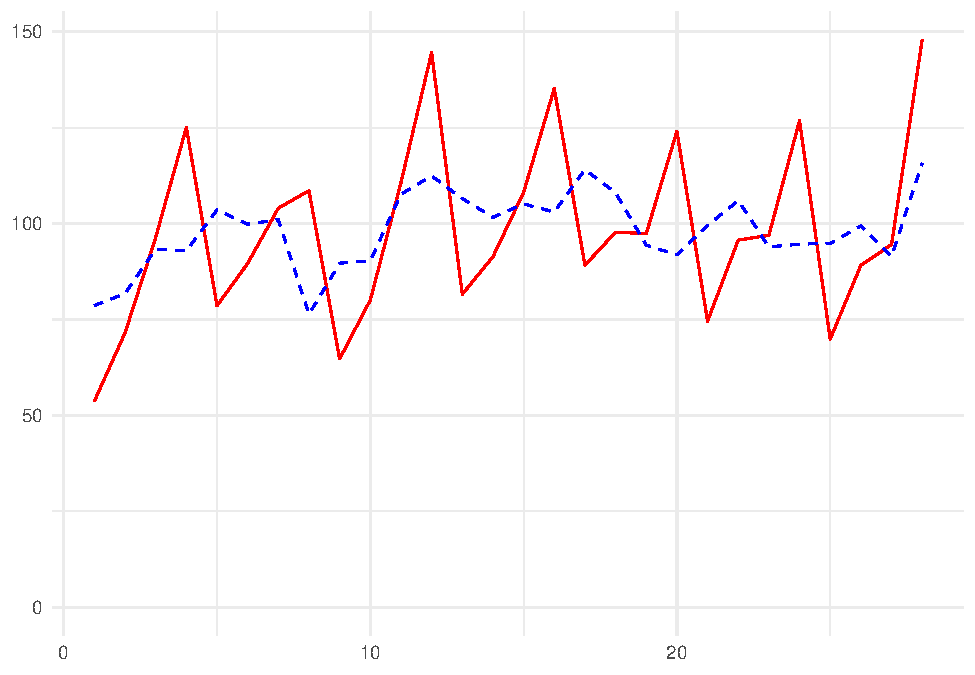
\includegraphics{rEkonometri_files/figure-latex/unnamed-chunk-71-1.pdf}

Modeli daha da genişletebiliriz. Aşağıdaki bağımsız değişkenleri modele ekleyelim:

\begin{itemize}
\item
  \textbf{rpdi:} Reel kişisel harcanabilir gelir
\item
  \textbf{conf:} Tüketici güven endeksi
\end{itemize}

\begin{Shaded}
\begin{Highlighting}[]
\NormalTok{model <-}\StringTok{ }\KeywordTok{lm}\NormalTok{(}\DataTypeTok{formula =}\NormalTok{ sales }\OperatorTok{~}\StringTok{ }\NormalTok{d2 }\OperatorTok{+}\StringTok{ }\NormalTok{d3 }\OperatorTok{+}\StringTok{ }\NormalTok{d4 }\OperatorTok{+}\StringTok{ }\NormalTok{rpdi }\OperatorTok{+}\StringTok{ }\NormalTok{conf, }\DataTypeTok{data =}\NormalTok{ df3)}
\KeywordTok{summary}\NormalTok{(model)}
\end{Highlighting}
\end{Shaded}

\begin{verbatim}
## 
## Call:
## lm(formula = sales ~ d2 + d3 + d4 + rpdi + conf, data = df3)
## 
## Residuals:
##      Min       1Q   Median       3Q      Max 
## -13.5677  -5.8781   0.0709   5.1689  11.8362 
## 
## Coefficients:
##               Estimate Std. Error t value Pr(>|t|)    
## (Intercept) -152.92922   52.59149  -2.908 0.008157 ** 
## d2            15.04522    4.31538   3.486 0.002091 ** 
## d3            26.00247    4.32524   6.012 4.74e-06 ***
## d4            60.87226    4.42744  13.749 2.80e-12 ***
## rpdi           1.59890    0.37016   4.320 0.000276 ***
## conf           0.29391    0.08438   3.483 0.002107 ** 
## ---
## Signif. codes:  0 '***' 0.001 '**' 0.01 '*' 0.05 '.' 0.1 ' ' 1
## 
## Residual standard error: 8.048 on 22 degrees of freedom
## Multiple R-squared:  0.9054, Adjusted R-squared:  0.8839 
## F-statistic:  42.1 on 5 and 22 DF,  p-value: 1.532e-10
\end{verbatim}

Bu eklediğimiz değişkenler mevsimsel etkilerden arındırıldı mı?

Frisch-Waugh teoremine göre evet. Yani, modele mevimsel kuklaları katarak aslında bütün zaman serilerini mevsimsellikten arındırmış oluyoruz.

Yukarıdaki çıktı bize mevsimsel faktörleri yansıtan kesmelerin çeyrekten çeyreğe değiştiğini fakat rpdi ve conf eğim parametrelerinin baştan sona sabit kaldığını varsaymaktadır. Bu varsayımı kademeli eğim kuklaları ile test edelim.

\(Sales_t = \beta_1 + \beta_2D_{2t} + \beta_3D_{t3} + \beta_4RPDI_t + \beta_5CONF_t + \beta_6(D_2*RPDI_t) + \beta_7(D_3*RPDI_t) +\)

\(\beta_8(D_4*RPDI_t) + \beta_9(D_2*CONF_t) + \beta_{10}(D_3*CONF_t) + \beta_{11}(D_4*CONF_t) + \epsilon_t\)

Varsayımı test etmemizi sağlayacak olan \(\beta_6\)'dan \(\beta_{11}\)'e kadar olan kademeli eğim parametreleridir.

\begin{Shaded}
\begin{Highlighting}[]
\NormalTok{df3 }\OperatorTok\StringTok{ }
\StringTok{  }\KeywordTok{mutate}\NormalTok{(}\DataTypeTok{d2_rpdi =}\NormalTok{ d2}\OperatorTok{*}\NormalTok{rpdi,}
         \DataTypeTok{d3_rpdi =}\NormalTok{ d3}\OperatorTok{*}\NormalTok{rpdi,}
         \DataTypeTok{d4_rpdi =}\NormalTok{ d4}\OperatorTok{*}\NormalTok{rpdi,}
         \DataTypeTok{d2_conf =}\NormalTok{ d2}\OperatorTok{*}\NormalTok{conf,}
         \DataTypeTok{d3_conf =}\NormalTok{ d3}\OperatorTok{*}\NormalTok{conf,}
         \DataTypeTok{d4_conf =}\NormalTok{ d4}\OperatorTok{*}\NormalTok{conf)}

\NormalTok{model <-}\StringTok{ }\KeywordTok{lm}\NormalTok{(}\DataTypeTok{formula =}\NormalTok{ sales }\OperatorTok{~}\StringTok{ }\NormalTok{d2 }\OperatorTok{+}\StringTok{ }\NormalTok{d3 }\OperatorTok{+}\StringTok{ }\NormalTok{d4 }\OperatorTok{+}\StringTok{ }\NormalTok{rpdi }\OperatorTok{+}\StringTok{ }\NormalTok{conf }\OperatorTok{+}\StringTok{ }\NormalTok{d2_rpdi }\OperatorTok{+}\StringTok{ }\NormalTok{d3_rpdi }\OperatorTok{+}\StringTok{ }\NormalTok{d4_rpdi }\OperatorTok{+}\StringTok{ }\NormalTok{d2_conf }\OperatorTok{+}\StringTok{ }\NormalTok{d3_conf }\OperatorTok{+}\StringTok{ }\NormalTok{d4_conf, }\DataTypeTok{data =}\NormalTok{ df3)}
\KeywordTok{summary}\NormalTok{(model)}
\end{Highlighting}
\end{Shaded}

\begin{verbatim}
## 
## Call:
## lm(formula = sales ~ d2 + d3 + d4 + rpdi + conf + d2_rpdi + d3_rpdi + 
##     d4_rpdi + d2_conf + d3_conf + d4_conf, data = df3)
## 
## Residuals:
##      Min       1Q   Median       3Q      Max 
## -11.2537  -4.0821   0.0971   3.1040  14.5502 
## 
## Coefficients:
##               Estimate Std. Error t value Pr(>|t|)  
## (Intercept) -191.58462  107.98136  -1.774   0.0951 .
## d2           196.70196  221.26332   0.889   0.3872  
## d3           123.13869  163.43984   0.753   0.4621  
## d4            50.96447  134.78844   0.378   0.7103  
## rpdi           2.04979    0.79989   2.563   0.0209 *
## conf           0.28094    0.15690   1.791   0.0923 .
## d2_rpdi       -1.11058    1.40395  -0.791   0.4405  
## d3_rpdi       -1.21807    1.13419  -1.074   0.2988  
## d4_rpdi       -0.04987    1.01416  -0.049   0.9614  
## d2_conf       -0.29482    0.38178  -0.772   0.4512  
## d3_conf        0.06524    0.25986   0.251   0.8050  
## d4_conf        0.05787    0.20107   0.288   0.7772  
## ---
## Signif. codes:  0 '***' 0.001 '**' 0.01 '*' 0.05 '.' 0.1 ' ' 1
## 
## Residual standard error: 8.157 on 16 degrees of freedom
## Multiple R-squared:  0.9293, Adjusted R-squared:  0.8807 
## F-statistic: 19.12 on 11 and 16 DF,  p-value: 3.777e-07
\end{verbatim}

Kademeli eğim parametrelerinin hiçbiri istatistiksel olarak anlamlı çıkmamıştır. Bu bize rpdi ile conf parametrelerinin sezonlar arasında değişmediğini göstermektedir. Bunun yanında mevsimsel kuklaların da istatistiksel olarak anlamlı çıkmadığını görüyoruz. Dolayısıyla, moda satışlarında mevsimsel değişimler yoktur deriz ancak kademeli eğim parametrelerini modelden çıkardığımızda (bir önceki çıktı) güçlü bir mevimsel faktör olduğunu görürüz.

\hypertarget{paruxe7alux131-doux11frusal-regresyondaki-roluxfc}{%
\section{Parçalı Doğrusal Regresyondaki Rolü}\label{paruxe7alux131-doux11frusal-regresyondaki-roluxfc}}

Parçalı doğrusal regresyonu anlamak için Türkiye'ye ait Covid-19 verilerini kullanacağız. Bu veriler 98 vaka ve sonrasına ait 13 günü kapsamaktadır.

\begin{Shaded}
\begin{Highlighting}[]
\NormalTok{zaman <-}\StringTok{ }\KeywordTok{seq}\NormalTok{(}\DecValTok{1}\NormalTok{,}\DecValTok{13}\NormalTok{,}\DecValTok{1}\NormalTok{)}
\NormalTok{vaka <-}\StringTok{ }\KeywordTok{c}\NormalTok{(}\DecValTok{98}\NormalTok{, }\DecValTok{192}\NormalTok{, }\DecValTok{359}\NormalTok{, }\DecValTok{670}\NormalTok{, }\DecValTok{947}\NormalTok{, }\DecValTok{1236}\NormalTok{, }\DecValTok{1529}\NormalTok{, }\DecValTok{1872}\NormalTok{, }\DecValTok{2433}\NormalTok{, }\DecValTok{3629}\NormalTok{, }\DecValTok{5698}\NormalTok{, }\DecValTok{7402}\NormalTok{, }\DecValTok{9217}\NormalTok{)}
\NormalTok{df <-}\StringTok{ }\KeywordTok{data.frame}\NormalTok{(}\DataTypeTok{zaman =}\NormalTok{ zaman, }\DataTypeTok{vaka =}\NormalTok{ vaka)}

\KeywordTok{ggplot}\NormalTok{(df, }\KeywordTok{aes}\NormalTok{(}\DataTypeTok{x =} \KeywordTok{factor}\NormalTok{(zaman), }\DataTypeTok{y =}\NormalTok{ vaka)) }\OperatorTok{+}
\StringTok{  }\KeywordTok{geom_point}\NormalTok{() }\OperatorTok{+}
\StringTok{  }\KeywordTok{geom_vline}\NormalTok{(}\DataTypeTok{xintercept =} \DecValTok{9}\NormalTok{, }\DataTypeTok{linetype =} \StringTok{"dashed"}\NormalTok{) }\OperatorTok{+}
\StringTok{  }\KeywordTok{theme_minimal}\NormalTok{() }\OperatorTok{+}
\StringTok{  }\KeywordTok{labs}\NormalTok{(}\DataTypeTok{x =} \StringTok{"zaman"}\NormalTok{)}
\end{Highlighting}
\end{Shaded}

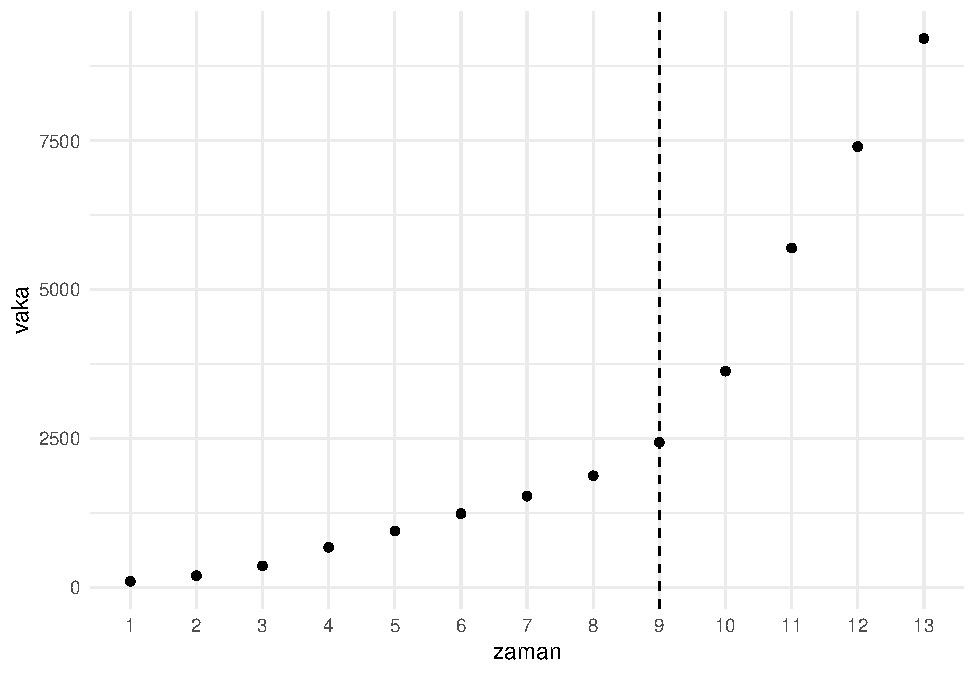
\includegraphics{rEkonometri_files/figure-latex/unnamed-chunk-74-1.pdf}

Vaka sayısının 9. güne kadar normal bir seyirde giderken bundan sonra yönünü yukarı kırdığını görüyoruz. Yani, iki farklı doğru görmekteyiz. 9. gün için eşik değer diyebiliriz. İşte bu bir parçalı doğrusal regresyondur ve bu parçaların kendilerine ait eğimleri vardır. Bu ayrıklığı hesaba katmak için kukla değişkenlerden yararlanacağız:

\(Y_i = \beta_1 + \beta_2X_i + \beta_3(X_i - X^*)D_i + \epsilon_i\)

Burada, Y vaka sayısı; X zaman ya da gündür. \(X^*\) zamanın önceden bilinen eşik değeridir ve D = 1 (\(X_i > X^*\)), D = 0 (\(X_i < X^*\)) olur. \(\beta_3\) istatistiksel olarak anlamlı ise farklı eğimler olduğu sonucuna ulaşırız.

Parçalara ayrılmış regresyon doğruları şöyle olur:

\(E(Y_i) = \beta_1 + \beta_2X_i, D_i = 0\) için

\(E(Y_i) = (\beta_1 - \beta_3X^*) + (\beta_2 + \beta_3)X_i, D_i = 1\) için

\(\beta_2\) eşikten önceki regresyon doğrusunun; \(\beta_2 + \beta_3\) ise eşikten sonraki regresyon doğrusunun eğimini verir.

\begin{Shaded}
\begin{Highlighting}[]
\NormalTok{df}\OperatorTok{$}\NormalTok{A <-}\StringTok{ }\NormalTok{df}\OperatorTok{$}\NormalTok{zaman }\OperatorTok{-}\StringTok{ }\DecValTok{9} \CommentTok{#eşik değerden çıkar.}
\NormalTok{df}\OperatorTok{$}\NormalTok{D <-}\StringTok{ }\KeywordTok{ifelse}\NormalTok{(df}\OperatorTok{$}\NormalTok{A }\OperatorTok{>}\StringTok{ }\DecValTok{0}\NormalTok{, }\DecValTok{1}\NormalTok{, }\DecValTok{0}\NormalTok{) }\CommentTok{#0'dan büyükse 1; değilse 0 ata.}
\NormalTok{df}\OperatorTok{$}\NormalTok{AD <-}\StringTok{ }\NormalTok{df}\OperatorTok{$}\NormalTok{A }\OperatorTok{*}\StringTok{ }\NormalTok{df}\OperatorTok{$}\NormalTok{D }\CommentTok{#her iki sütunu çarp.}

\NormalTok{model <-}\StringTok{ }\KeywordTok{lm}\NormalTok{(}\DataTypeTok{formula =}\NormalTok{ vaka }\OperatorTok{~}\StringTok{ }\NormalTok{zaman }\OperatorTok{+}\StringTok{ }\NormalTok{AD, }\DataTypeTok{data =}\NormalTok{ df)}
\KeywordTok{summary}\NormalTok{(model)}
\end{Highlighting}
\end{Shaded}

\begin{verbatim}
## 
## Call:
## lm(formula = vaka ~ zaman + AD, data = df)
## 
## Residuals:
##     Min      1Q  Median      3Q     Max 
## -257.84  -71.39   -7.90   45.57  307.69 
## 
## Coefficients:
##             Estimate Std. Error t value Pr(>|t|)    
## (Intercept)  -365.27     106.90  -3.417  0.00658 ** 
## zaman         276.73      18.05  15.329 2.84e-08 ***
## AD           1484.80      51.56  28.796 5.94e-11 ***
## ---
## Signif. codes:  0 '***' 0.001 '**' 0.01 '*' 0.05 '.' 0.1 ' ' 1
## 
## Residual standard error: 151 on 10 degrees of freedom
## Multiple R-squared:  0.9978, Adjusted R-squared:  0.9974 
## F-statistic:  2286 on 2 and 10 DF,  p-value: 4.948e-14
\end{verbatim}

Tahmin edilen bütün regresyon parametreleri tek tek (t) ve toplu (F) olarak istatistiksel açıdan anlamlıdır. İki regresyon doğrusunun da eğim parametrelerinin farklı olduğunu söyleyebiliriz.

Ortalama Vaka Sayısı = -365.27 + 276.73Zaman, Zaman \textless{} 9

Ortalama Vaka Sayısı = (-365.27 - 1484.80*9) + (276.73 + 1484.80)Zaman, Zaman \textgreater{} 9

Ortalama Vaka sayısı = -13728.47 + 1761.53Zaman, Zaman \textgreater{} 9

Eşik güne kadar zamandaki birim artış başına birim vaka sayısı 277 artarken; eşikten sonra 1762 artmıştır.

\begin{Shaded}
\begin{Highlighting}[]
\CommentTok{#Paket yardımı ile aşağıdaki gibi bulunabilir:}
\NormalTok{model <-}\StringTok{ }\KeywordTok{segmented}\NormalTok{(}\DataTypeTok{obj =} \KeywordTok{lm}\NormalTok{(vaka }\OperatorTok{~}\StringTok{ }\NormalTok{zaman, }\DataTypeTok{data =}\NormalTok{ df), }\DataTypeTok{seg.Z =} \OperatorTok{~}\NormalTok{zaman, }\DataTypeTok{psi =} \KeywordTok{list}\NormalTok{(}\DataTypeTok{zaman =} \DecValTok{9}\NormalTok{)) }\CommentTok{#Kırılma birden fazla ise c(...) ile eklenebilir.}
\CommentTok{#summary(model)}
\CommentTok{#slope(model)}
\end{Highlighting}
\end{Shaded}

\hypertarget{uxe7oklu-doux11frusal-baux11flantux131}{%
\chapter{Çoklu Doğrusal Bağlantı}\label{uxe7oklu-doux11frusal-baux11flantux131}}

Bağımsız değişkenler arasında tam ya da tama yakın doğrusal bir ilişki yoktur. Eğer bağımsız değişkenler arasında böyle bir ilişki varsa çoklu doğrusal bağlantı olarak tanımlanabilir.

Öncelikle tam bir doğrusal bağlantı olduğu durumda Sıradan En Küçük Kareler tahminlerinin elde edilmesi mekanik olarak olanaksızdır. Bununla birlikte bağımsız değişkenler arasında tama yakın bir doğrusal bir ilişki de bulunabilir. Kennedy'nin altını çizdiği şu nokta önemlidir: \emph{Çoklu doğrusallık bağımsız değişkenler arasındaki teorik ya da gerçek doğrusal ilişkinin var olup olmamasına bağlı değildir; varlığı üzerinde çalışılan veri kümesinde yaklaşık doğrusal bir ilişkinin var olup olmadığı ile ilgilidir.}

Çoklu doğrusal bağlantı varsa neler olur?

\begin{itemize}
\item
  Sıradan En Küçük Kareler tahmincileri BLUE'dur (Best Linear Unbiased Estimator, En İyi Doğrusal Yansız Tahmin Edici). Fakat hassas tahmini zorlaştıran büyük varyans ve kovaryanslar olacaktır.
\item
  Güven aralıkları daha geniş olma eğiliminde olacaktır. Bunun sonucu olarak gerçek anakütle parametresinin sıfır olduğunu söyleyen \(H_0\)'ı reddedemeyebiliriz.
\item
  En az bir parametrenin t oranı istatistiksel olarak anlamlı çıkmama eğiliminde olacaktır.
\item
  Regresyon parametreleri istatistiksel olarak anlamlı olmamasına rağmen \(R^2\) değeri yüksek çıkabilir.
\item
  Sıradan En Küçük Kareler tahmincileri ve bunların standart hataları verilerdeki küçük değişimlere duyarlı olabilir.
\item
  Seçilen regresyon modeline doğrusal bağlantılı bir değişken eklemek modeldeki diğer değişkenlere ait parametre değerlerini değiştirebilecektir.
\end{itemize}

\begin{Shaded}
\begin{Highlighting}[]
\KeywordTok{library}\NormalTok{(corrplot);}\KeywordTok{library}\NormalTok{(psych);}\KeywordTok{library}\NormalTok{(car);}\KeywordTok{library}\NormalTok{(factoextra);}\KeywordTok{library}\NormalTok{(FactoMineR);}\KeywordTok{library}\NormalTok{(lmridge);}\KeywordTok{library}\NormalTok{(tidyverse)}

\KeywordTok{setwd}\NormalTok{(}\StringTok{"C:/Users/datanerd/Desktop/Github/rEkonometri/data"}\NormalTok{)}
\NormalTok{df1 <-}\StringTok{ }\KeywordTok{read.table}\NormalTok{(}\StringTok{"yagis.txt"}\NormalTok{, }\DataTypeTok{sep =} \StringTok{" "}\NormalTok{, }\DataTypeTok{header =} \OtherTok{TRUE}\NormalTok{)}
\NormalTok{df2 <-}\StringTok{ }\KeywordTok{read.table}\NormalTok{(}\StringTok{"yumurta.txt"}\NormalTok{, }\DataTypeTok{sep =} \StringTok{" "}\NormalTok{, }\DataTypeTok{header =} \OtherTok{TRUE}\NormalTok{)}
\end{Highlighting}
\end{Shaded}

10 tane istasyona ait yıllık yağış (mm) verileri ile havza yıllık getirisi (mm) aşağıdaki gibidir:

\begin{Shaded}
\begin{Highlighting}[]
\NormalTok{df1}
\end{Highlighting}
\end{Shaded}

\begin{verbatim}
##    Year   x1   x2   x3   x4   x5   x6   x7   x8   x9  x10      y
## 1  1979 1948 4177 5496 2922 5713 3640 3203 2739 2167 2299 3255.2
## 2  1980 2261 3670 7797 3327 6934 4424 3692 3451 2866 2653 3682.7
## 3  1981 1989 4353 7392 2837 6275 4827 4476 4403 3568 3241 3921.9
## 4  1982 1999 3307 7061 3439 6641 4815 4256 4129 3447 3046 3909.3
## 5  1983 2086 4230 6564 2987 6675 3959 3900 3559 4078 3583 3768.9
## 6  1984 1717 2714 5919 3394 5605 3648 3085 2440 2631 2587 3106.4
## 7  1985 1383 2357 5053 2958 5144 3106 4052 3006 3049 2890 3069.4
## 8  1986 1470 3004 3951 2691 5116 3557 2775 1909 1952 1723 2940.2
## 9  1987 1350 2446 4280 2397 4722 3556 2818 2945 2931 2733 3015.3
## 10 1988 1602 4188 5910 3619 6869 5142 3190 3660 3964 3107 3953.2
## 11 1989 1417 3631 5145 3282 5226 3793 2663 3017 2579 3367 3172.4
## 12 1990 1662 4683 6384 6376 7313 4679 3037 3666 3142 2621 3791.0
## 13 1991 1955 4553 5679 6141 6068 3651 2601 2791 2148 2448 3344.8
## 14 1992 1974 3836 6021 5646 5876 4026 3037 3920 2583 2742 3650.3
## 15 1993 2094 4183 6733 6720 6044 6573 2465 3406 2410 2539 3878.7
## 16 1994 3149 6128 8151 9048 8384 7467 2888 3522 2496 2895 4606.2
## 17 1995 1471 2952 4151 4975 5149 4733 2603 3493 3396 3554 3498.8
## 18 1996 1691 3711 4200 4962 5359 3782 3185 3099 3381 2938 3241.0
## 19 1997 2373 4836 6704 6563 6197 5001 3902 3685 3636 3365 4013.5
\end{verbatim}

Çoklu doğrusal bağlantıyı tespit edelim.

Önce bir model kuralım.

\begin{Shaded}
\begin{Highlighting}[]
\NormalTok{model <-}\StringTok{ }\KeywordTok{lm}\NormalTok{(y }\OperatorTok{~}\NormalTok{., df1[,}\OperatorTok{-}\DecValTok{1}\NormalTok{]) }\CommentTok{#yıl sütunu hariç.}
\KeywordTok{summary}\NormalTok{(model)}
\end{Highlighting}
\end{Shaded}

\begin{verbatim}
## 
## Call:
## lm(formula = y ~ ., data = df1[, -1])
## 
## Residuals:
##      Min       1Q   Median       3Q      Max 
## -126.482  -28.635   -0.011   21.701   72.102 
## 
## Coefficients:
##               Estimate Std. Error t value Pr(>|t|)   
## (Intercept) 782.347374 209.902668   3.727  0.00581 **
## x1            0.186129   0.112160   1.659  0.13560   
## x2            0.048356   0.041101   1.177  0.27321   
## x3           -0.019849   0.045533  -0.436  0.67441   
## x4            0.001912   0.019025   0.101  0.92240   
## x5            0.119623   0.055763   2.145  0.06426 . 
## x6            0.155540   0.032434   4.796  0.00136 **
## x7            0.023158   0.065288   0.355  0.73198   
## x8            0.194765   0.061793   3.152  0.01356 * 
## x9            0.079910   0.075390   1.060  0.32012   
## x10          -0.004085   0.076757  -0.053  0.95886   
## ---
## Signif. codes:  0 '***' 0.001 '**' 0.01 '*' 0.05 '.' 0.1 ' ' 1
## 
## Residual standard error: 72.81 on 8 degrees of freedom
## Multiple R-squared:  0.9877, Adjusted R-squared:  0.9723 
## F-statistic: 64.28 on 10 and 8 DF,  p-value: 1.537e-06
\end{verbatim}

\begin{itemize}
\tightlist
\item
  Yüksek \(R^2\) fakat az sayıda anlamlı t oranı ya da en az bir parametrenin t oranının istatistiksel olarak anlamlı çıkmaması:
\end{itemize}

Uygulamamızda \(R^2\) değeri olan \%99 yüksektir. Birçok t oranı istatistiksel olarak anlamlı çıkmadı.

\begin{itemize}
\tightlist
\item
  Bağımsız değişkenler arasındaki yüksek ikili korelasyonlar:
\end{itemize}

\begin{Shaded}
\begin{Highlighting}[]
\KeywordTok{corrplot}\NormalTok{(}\KeywordTok{cor}\NormalTok{(df1[,}\OperatorTok{-}\KeywordTok{c}\NormalTok{(}\DecValTok{1}\NormalTok{,}\DecValTok{12}\NormalTok{)]), }\DataTypeTok{method =} \StringTok{"number"}\NormalTok{, }\DataTypeTok{type =} \StringTok{"lower"}\NormalTok{)}
\end{Highlighting}
\end{Shaded}

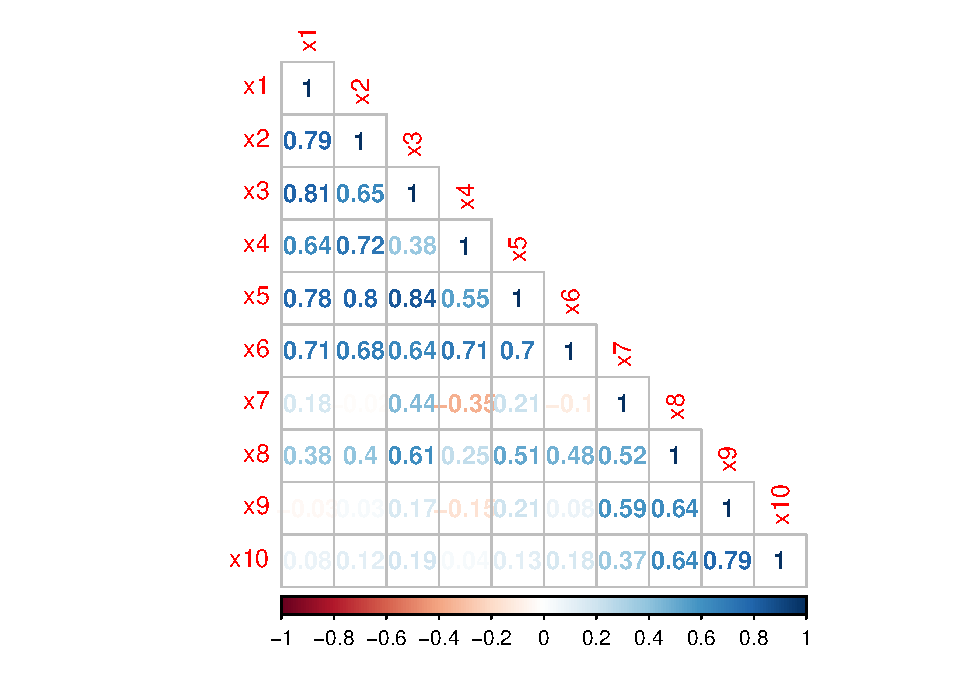
\includegraphics{rEkonometri_files/figure-latex/unnamed-chunk-80-1.pdf}

Söylendiği üzere yüksek korelasyonlar göze çarpıyor fakat ikili değişkenli korelasyon parametrelerine ne kadar güveneceğiz? Çünkü bu korelasyonlar hesaplanırken modeldeki diğer değişkenler sabit kalmaz.

\begin{itemize}
\tightlist
\item
  Kısmi korelasyon parametreleri:
\end{itemize}

Yukarıda diğer değişkenlerin sabit kalmayacağından bahsetmiştik. Üç tane değişkenimiz (\(x_1, x_2, x_3\)) olduğunu varsayalım. \(x_2\) ile \(x_3\) arasında \%90'lık bir korelasyon olabilir. Fakat burada \(x_1\)'in etkisini hesaba katmadık. \(x_1\) değişkeni hem \(x_2\)'yi hem de \(x_3\)'ü etkiliyor olabilir. Yani, \(x_2\) ile \(x_3\) arasındaki yüksek korelasyon \(x_1\)'in her ikisini etkiliyor olmasından kaynaklı olabilir. Kısmi korelasyon ile \(x_1\)'in etkisi çıkarılarak \(x_2\) ve \(x_3\) arasındaki korelasyon hesaplanır. Bu değer de örneğin \%30'a düşebilir.

\begin{Shaded}
\begin{Highlighting}[]
\KeywordTok{corrplot}\NormalTok{(}\KeywordTok{partial.r}\NormalTok{(df1[,}\OperatorTok{-}\KeywordTok{c}\NormalTok{(}\DecValTok{1}\NormalTok{,}\DecValTok{12}\NormalTok{)]), }\DataTypeTok{method =} \StringTok{"number"}\NormalTok{, }\DataTypeTok{type =} \StringTok{"lower"}\NormalTok{)}
\end{Highlighting}
\end{Shaded}

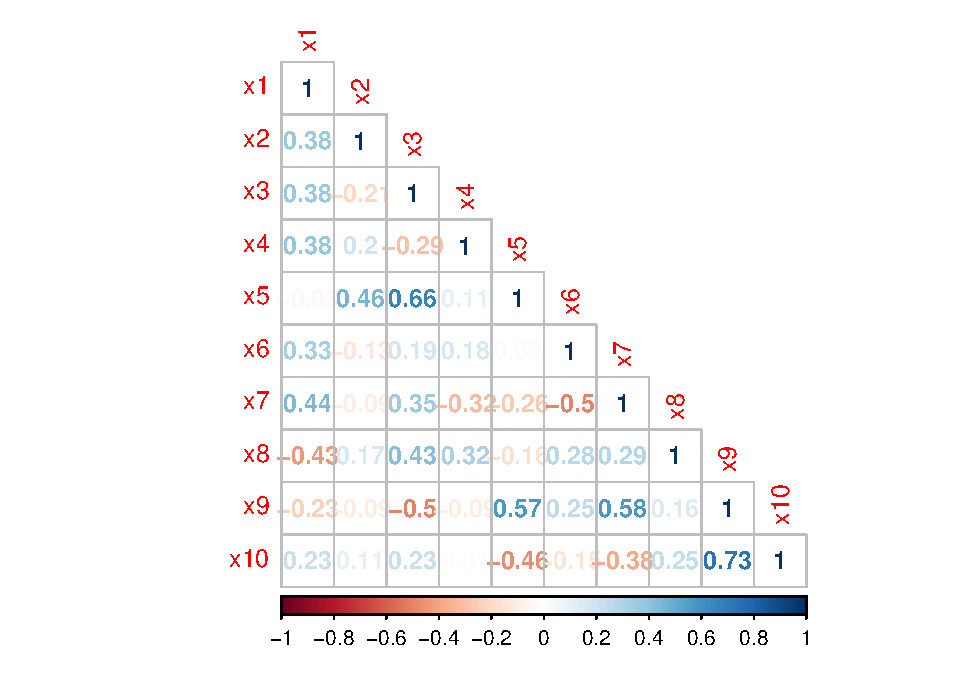
\includegraphics{rEkonometri_files/figure-latex/unnamed-chunk-81-1.pdf}

Mesela, \(x_1\)-\(x_2\) korelasyonu \%79 iken kısmi korelasyon ile \%38'e düştü. İki değişken arasındaki basit korelasyon parametresi anlamlı, fakat kısmi korelasyon parametresi anlamsız ise bu durum çoklu doğrusal bağlantı problemi için bir işaret olabilir. Kısmi korelasyon yaklaşımı her zaman etkili olmamaktadır. Diğer bir anlatımla, kısmi korelasyon parametreleri yüksek olması durumunda bile çoklu doğrusal bağlantı problemi olabilmektedir.

\begin{itemize}
\tightlist
\item
  Yan regresyon hesaplamaları:
\end{itemize}

Modele eklenen diğer bağımsız değişkenlerin hangi bağımsız değişkenlerle yüksek derecede doğrusal bağlantılı olduğunu ortaya koymak için her bir bağımsız değişkenin geriye kalan bağımsız değişkenlere göre regresyonu hesaplanır. Uygulamamızda 10 tane bağımsız değişken vardır. Bundan dolayı 10 tane yan regresyonumuz olacaktır. Burada F testi kullanılır. \(H_0\) reddedilirse doğrusal bağlantı sonucuna ulaşılır. Oldukça yorucu bir yöntem olabilir.

\begin{itemize}
\tightlist
\item
  Varyans şişirme faktörü ve tolerans faktörü: Varyans şişirme faktörü ile parametre tahminlerinin ve varyanslarının çoklu doğrusal bağlantı nedeni ile gerçek değerlerinden ne kadar uzaklaştığı belirlenir. VIF'lerin hesaplanmasını göstermek için aşağıdaki gibi üç bağımsız değişkenli bir regresyon modelini inceleyelim:
\end{itemize}

\(Y_i = \beta_1 + \beta_2X_1 + \beta_3X_2 + \beta_4X_3 + \epsilon_i\)

Adım-1: \(X_1\) bağımlı; \(X_2\) ve \(X_3\) bağımsız. \(R^2\) hesapla. \(X_1\) için \(VIF = \frac{1}{(1 – R^2)}\)

Adım-2: \(X_2\) bağımlı; \(X_1\) ve \(X_3\) bağımsız. \(R^2\) hesapla. \(X_2\) için \(VIF = \frac{1}{(1 – R^2)}\)

Adım-3: \(X_3\) bağımlı; \(X_1\) ve \(X_2\) bağımsız. \(R^2\) hesapla. \(X_3\) için \(VIF = \frac{1}{(1 – R^2)}\)

Bağımlı değişken ile bağımsız değişkenler arasında ilişki yoksa (bu durumda \(R^2\) = 0) VIF \(\frac{1}{(1 – 0)}\)'dan 1'e eşit olacaktır. Eğer tam bir ilişki varsa (bu durumda \(R^2\) = 1) VIF \(\frac{1}{(1 – 1)}\)'den \(\infty\)'a eşit olacaktır. \(R^2\) = 0.9 (ya da \%90) ise VIF 10 olacaktır. Literatürde yer alan pratik bir kurala göre VIF \textgreater{} 10 için çoklu doğrusal bağlantı deniliyor. Tolerans değeri ise 1'den \(R^2\) değerinin çıkarılması ile bulunur. Daha küçük tolerans daha büyük VIF demektir. Küçük veri setlerinde VIF \textgreater{} 5'de bile çoklu doğrusal bağlantı bulunabilir.

\begin{Shaded}
\begin{Highlighting}[]
\NormalTok{car}\OperatorTok{::}\KeywordTok{vif}\NormalTok{(model)}
\end{Highlighting}
\end{Shaded}

\begin{verbatim}
##        x1        x2        x3        x4        x5        x6        x7        x8 
##  8.057920  4.934190 11.000217  4.188910  8.837753  4.254056  5.365104  4.658428 
##        x9       x10 
##  7.457020  4.278819
\end{verbatim}

Düzeltici önlemler için temel bileşenler analizi ve hemen arkasından temel bileşenler regresyonu konularını inceleyeceğiz. Akabinde de ridge regresyona bakacağız.

Aslında düzeltici önemlerden biri hiçbir şey yapmamaktır. Blanchard, çoklu doğrusallık için \emph{Sıradan En Küçük Kareler'in ya da daha genel olarak istatistiğin bir sorunu değil, Tanrı buyruğudur} der.

Bu da bir seçenek olabileceği gibi biz temel bileşenler analizi ve regresyonu ile girişimizi yapalım.

\hypertarget{temel-bileux15fenler-analiziregresyonu}{%
\section{Temel Bileşenler Analizi/Regresyonu}\label{temel-bileux15fenler-analiziregresyonu}}

Temel bileşenler analizi, korelasyonlu değişkenleri korelasyonsuz değişkenlere (ortogonal değişkenler) dönüştürebilmektedir. Bu şekilde elde edilen değişkenlere temel bileşenler denir. Analizin temel düşüncesi şudur: Korelasyonlu değişkenler alt gruplara ayrılır. Herhangi bir alt gruba ait olan değişkenler bunları bir arada hareket ettiren ortak bir faktöre sahip olur. Bu ortak faktör temel bileşendir.

Basit bir ifade ile, 10 tane bağımsız değişkenimiz vardı. Biz boyut indirgeme yaparak daha az sayıda değişkenle (birbirleriyle korelasyonsuz) bağımlı değişkeni tahmin etmeye çalışacağız. Yani, örneğin fazla bilgi kaybetmeden birkaç GB veri boyutunu birkaç MB boyutuna düşürebiliriz.

Değişkenlere boyut indirgedikten sonra elde ettiğimiz değişkenlere regresyon modeli kuracağız. Buna ise temel bileşenler regresyonu denir.

Temel bileşenler analizi ile başlayalım. Burada örneğimizi basit bir şekilde anlatabilmek için değiştiriyoruz.

Adım-1: Elimizde 15 yıla ait rainfall (cm) ve runoff (cm) verileri olsun. Değerler şöyle;

\begin{Shaded}
\begin{Highlighting}[]
\NormalTok{rainfall <-}\StringTok{ }\KeywordTok{c}\NormalTok{(}\DecValTok{105}\NormalTok{,}\DecValTok{115}\NormalTok{,}\DecValTok{103}\NormalTok{,}\DecValTok{94}\NormalTok{,}\DecValTok{95}\NormalTok{,}\DecValTok{104}\NormalTok{,}\DecValTok{120}\NormalTok{,}\DecValTok{121}\NormalTok{,}\DecValTok{127}\NormalTok{,}\DecValTok{79}\NormalTok{,}\DecValTok{133}\NormalTok{,}\DecValTok{111}\NormalTok{,}\DecValTok{127}\NormalTok{,}\DecValTok{108}\NormalTok{,}\DecValTok{85}\NormalTok{)}
\NormalTok{runoff <-}\StringTok{ }\KeywordTok{c}\NormalTok{(}\DecValTok{42}\NormalTok{,}\DecValTok{46}\NormalTok{,}\DecValTok{26}\NormalTok{,}\DecValTok{39}\NormalTok{,}\DecValTok{29}\NormalTok{,}\DecValTok{33}\NormalTok{,}\DecValTok{48}\NormalTok{,}\DecValTok{58}\NormalTok{,}\DecValTok{45}\NormalTok{,}\DecValTok{20}\NormalTok{,}\DecValTok{54}\NormalTok{,}\DecValTok{37}\NormalTok{,}\DecValTok{39}\NormalTok{,}\DecValTok{34}\NormalTok{,}\DecValTok{25}\NormalTok{)}
\NormalTok{df <-}\StringTok{ }\KeywordTok{data.frame}\NormalTok{(}\DataTypeTok{rainfall =}\NormalTok{ rainfall, }\DataTypeTok{runoff =}\NormalTok{ runoff)}
\end{Highlighting}
\end{Shaded}

Adım-2: Verilerin matrise aktarılması ve ortalamadan sapmalarının alınması.

\begin{Shaded}
\begin{Highlighting}[]
\NormalTok{df}\OperatorTok{$}\NormalTok{rainfalldev <-}\StringTok{ }\KeywordTok{round}\NormalTok{(df}\OperatorTok{$}\NormalTok{rainfall }\OperatorTok{-}\StringTok{ }\KeywordTok{mean}\NormalTok{(df}\OperatorTok{$}\NormalTok{rainfall), }\DataTypeTok{digits =} \DecValTok{1}\NormalTok{)}
\NormalTok{df}\OperatorTok{$}\NormalTok{runoffdev <-}\StringTok{ }\KeywordTok{round}\NormalTok{(df}\OperatorTok{$}\NormalTok{runoff }\OperatorTok{-}\StringTok{ }\KeywordTok{mean}\NormalTok{(df}\OperatorTok{$}\NormalTok{runoff), }\DataTypeTok{digits =} \DecValTok{1}\NormalTok{)}
\end{Highlighting}
\end{Shaded}

Adım-3: Kovaryans matrisinin hesaplanması.

\begin{Shaded}
\begin{Highlighting}[]
\NormalTok{covmatrix <-}\StringTok{ }\KeywordTok{cov}\NormalTok{(df[,}\KeywordTok{c}\NormalTok{(}\DecValTok{3}\NormalTok{,}\DecValTok{4}\NormalTok{)])}
\NormalTok{covmatrix}
\end{Highlighting}
\end{Shaded}

\begin{verbatim}
##             rainfalldev runoffdev
## rainfalldev    249.9810  141.0476
## runoffdev      141.0476  117.5238
\end{verbatim}

Adım-4: Özdeğerler ve özvektörlerin hesaplanması.

\begin{Shaded}
\begin{Highlighting}[]
\NormalTok{A <-}\StringTok{ }\KeywordTok{matrix}\NormalTok{(}\KeywordTok{c}\NormalTok{(}\FloatTok{249.9810}\NormalTok{, }\FloatTok{141.0476}\NormalTok{, }\FloatTok{141.0476}\NormalTok{, }\FloatTok{117.5238}\NormalTok{), }\DecValTok{2}\NormalTok{, }\DecValTok{2}\NormalTok{, }\DataTypeTok{byrow =} \OtherTok{TRUE}\NormalTok{)}
\NormalTok{eigen <-}\StringTok{ }\KeywordTok{eigen}\NormalTok{(A)}
\NormalTok{eigen}
\end{Highlighting}
\end{Shaded}

\begin{verbatim}
## eigen() decomposition
## $values
## [1] 339.5749  27.9299
## 
## $vectors
##            [,1]       [,2]
## [1,] -0.8441048  0.5361782
## [2,] -0.5361782 -0.8441048
\end{verbatim}

Adım-5: Temel bileşenlerin açıklama oranlarının hesaplanması.

\begin{Shaded}
\begin{Highlighting}[]
\NormalTok{eigen}\OperatorTok{$}\NormalTok{values[}\DecValTok{1}\NormalTok{] }\OperatorTok{/}\StringTok{ }\NormalTok{(eigen}\OperatorTok{$}\NormalTok{values[}\DecValTok{1}\NormalTok{] }\OperatorTok{+}\StringTok{ }\NormalTok{eigen}\OperatorTok{$}\NormalTok{values[}\DecValTok{2}\NormalTok{])}
\end{Highlighting}
\end{Shaded}

\begin{verbatim}
## [1] 0.9240013
\end{verbatim}

\begin{Shaded}
\begin{Highlighting}[]
\NormalTok{eigen}\OperatorTok{$}\NormalTok{values[}\DecValTok{2}\NormalTok{] }\OperatorTok{/}\StringTok{ }\NormalTok{(eigen}\OperatorTok{$}\NormalTok{values[}\DecValTok{1}\NormalTok{] }\OperatorTok{+}\StringTok{ }\NormalTok{eigen}\OperatorTok{$}\NormalTok{values[}\DecValTok{2}\NormalTok{])}
\end{Highlighting}
\end{Shaded}

\begin{verbatim}
## [1] 0.07599872
\end{verbatim}

Birinci temel bileşen varyansın \%92.4'ünü açıklarken; ikinci temel bileşen \%7.6'sını açıklıyor. Temel bileşenler, değişkenlerin (örneğimizde rainfall ve runoff) doğrusal bir kombinasyonudur. Yani, rainfall \(λ_1\) ve runoff \(λ_2\)'dir ya da tam tersi.

Yazının başındaki veri setine dönelim.

Temel bileşenler analizinde ilk olarak standartlaştırılma işlemi yapılır (farklı ölçümlü verilerin yer alması). Yani, tüm hesaplamalar standart veriler üzerinden yapılır. Bağımlı değişken Y için ise merkezileştirme yapılır. Yani, Y değerlerinden Y ortalama değerleri çıkartılır. Bunu, model kurarken kesme terimine ihtiyacımız kalmaması için yapıyoruz. Bunu yapmak kesin bir kural değildir.

\begin{Shaded}
\begin{Highlighting}[]
\NormalTok{df1_yeni <-}\StringTok{ }\NormalTok{df1[,}\KeywordTok{c}\NormalTok{(}\DecValTok{2}\OperatorTok{:}\DecValTok{11}\NormalTok{)] }\CommentTok{#Sadece X'ler alındı.}
\NormalTok{df1_yeni <-}\StringTok{ }\KeywordTok{as.data.frame}\NormalTok{(}\KeywordTok{apply}\NormalTok{(df1_yeni, }\DataTypeTok{MARGIN =} \DecValTok{2}\NormalTok{, }\DataTypeTok{FUN =} \ControlFlowTok{function}\NormalTok{(x) }\KeywordTok{scale}\NormalTok{(x))) }\CommentTok{#Standardize edildi.}
\NormalTok{df1_yeni}\OperatorTok{$}\NormalTok{y <-}\StringTok{ }\NormalTok{df1}\OperatorTok{$}\NormalTok{y }\OperatorTok{-}\StringTok{ }\KeywordTok{mean}\NormalTok{(df1}\OperatorTok{$}\NormalTok{y) }\CommentTok{#Merkezileştirildi.}
\NormalTok{df1_yeni}
\end{Highlighting}
\end{Shaded}

\begin{verbatim}
##            x1           x2           x3         x4           x5         x6
## 1   0.1721888  0.363397603 -0.343849487 -0.8200257 -0.389046112 -0.7339610
## 2   0.8928130 -0.183230928  1.496820983 -0.6006661  0.945491926 -0.0155772
## 3   0.2665837  0.553154253  1.172843781 -0.8660641  0.225213001  0.3536941
## 4   0.2896068 -0.574604018  0.908062414 -0.5400037  0.625246516  0.3426984
## 5   0.4899081  0.420540231  0.510490392 -0.7848198  0.662408100 -0.4416594
## 6  -0.3596456 -1.213954549 -0.005473299 -0.5643770 -0.507088789 -0.7266306
## 7  -1.1286184 -1.598858662 -0.698224549 -0.8005271 -1.010956140 -1.2232683
## 8  -0.9283171 -0.901287342 -1.579762514 -0.9451419 -1.041559796 -0.8100144
## 9  -1.2045947 -1.502902175 -1.316581035 -1.1043807 -1.472196968 -0.8109307
## 10 -0.6244117  0.375257394 -0.012672792 -0.4425106  0.874447723  0.6423304
## 11 -1.0503397 -0.225279276 -0.624629728 -0.6250394 -0.921331144 -0.5937662
## 12 -0.4862729  0.908947972  0.366500525  1.0507595  1.359734282  0.2180808
## 13  0.1883050  0.768786810 -0.197459789  0.9234767 -0.001035462 -0.7238816
## 14  0.2320490 -0.004255906  0.076120959  0.6553706 -0.210889109 -0.3802669
## 15  0.5083266  0.369866580  0.645680878  1.2370797 -0.027267168  1.9535641
## 16  2.9372675  2.466893194  1.780001055  2.4979911  2.530324158  2.7727416
## 17 -0.9260148 -0.957351806 -1.419773773  0.2919378 -1.005491201  0.2675613
## 18 -0.4195058 -0.139026254 -1.380576531  0.2848966 -0.775963774 -0.6038456
## 19  1.1506721  1.073906878  0.622482511  1.1520440  0.139959957  0.5131313
##             x7         x8          x9         x10          y
## 1  -0.08393555 -0.9481675 -1.29125899 -1.21196071 -314.23158
## 2   0.71920060  0.2396101 -0.16679432 -0.44654778  113.26842
## 3   2.00684630  1.8277621  0.96249637  0.82481608  352.46842
## 4   1.64551715  1.3706679  0.76784655  0.40319031  339.86842
## 5   1.06082089  0.4197786  1.78292124  1.56428282  199.46842
## 6  -0.27773937 -1.4469674 -0.54483323 -0.58925189 -463.03158
## 7   1.31046648 -0.5027509  0.12759342  0.06588970 -500.03158
## 8  -0.78688499 -2.3327959 -1.63712437 -2.45737837 -629.23158
## 9  -0.71626156 -0.6045128 -0.06223037 -0.27357310 -554.13158
## 10 -0.10528682  0.5882695  1.59953215  0.53508350  383.76842
## 11 -0.97083437 -0.4844004 -0.62848439  1.09725119 -397.03158
## 12 -0.35657482  0.5982789  0.27720031 -0.51573765  221.56842
## 13 -1.07266350 -0.8614197 -1.32182384 -0.88979538 -224.63158
## 14 -0.35657482  1.0220085 -0.62204969 -0.25411345   80.86842
## 15 -1.29603061  0.1645399 -0.90035067 -0.69303669  309.26842
## 16 -0.60129320  0.3580542 -0.76200452  0.07670061 1036.76842
## 17 -1.06937869  0.3096756  0.68580407  1.50157950  -70.63158
## 18 -0.11349885 -0.3476058  0.66167392  0.16967450 -328.43158
## 19  1.06410570  0.6299752  1.07188635  1.09292683  444.06842
\end{verbatim}

Kovaryans matrisini aşağıdaki gibi oluşturalım.

\begin{Shaded}
\begin{Highlighting}[]
\NormalTok{cov_m <-}\StringTok{ }\KeywordTok{cov}\NormalTok{(df1_yeni[,}\OperatorTok{-}\DecValTok{11}\NormalTok{])}
\NormalTok{cov_m}
\end{Highlighting}
\end{Shaded}

\begin{verbatim}
##              x1          x2        x3          x4        x5         x6
## x1   1.00000000  0.79404489 0.8099080  0.63970323 0.7752141  0.7129395
## x2   0.79404489  1.00000000 0.6463593  0.72026928 0.7965001  0.6830817
## x3   0.80990796  0.64635934 1.0000000  0.37713523 0.8405912  0.6367616
## x4   0.63970323  0.72026928 0.3771352  1.00000000 0.5453583  0.7086409
## x5   0.77521414  0.79650014 0.8405912  0.54535834 1.0000000  0.7019490
## x6   0.71293954  0.68308169 0.6367616  0.70864090 0.7019490  1.0000000
## x7   0.17691772 -0.01513445 0.4366362 -0.35274604 0.2114573 -0.1030525
## x8   0.37593752  0.39791947 0.6147578  0.24628053 0.5117468  0.4794635
## x9  -0.03410999  0.03326402 0.1690332 -0.15071195 0.2054040  0.0833055
## x10  0.08058727  0.12261396 0.1865701  0.03522937 0.1251372  0.1797110
##              x7        x8          x9        x10
## x1   0.17691772 0.3759375 -0.03410999 0.08058727
## x2  -0.01513445 0.3979195  0.03326402 0.12261396
## x3   0.43663616 0.6147578  0.16903324 0.18657010
## x4  -0.35274604 0.2462805 -0.15071195 0.03522937
## x5   0.21145731 0.5117468  0.20540401 0.12513717
## x6  -0.10305249 0.4794635  0.08330550 0.17971098
## x7   1.00000000 0.5187275  0.59255388 0.36865464
## x8   0.51872746 1.0000000  0.63756523 0.63699489
## x9   0.59255388 0.6375652  1.00000000 0.78544619
## x10  0.36865464 0.6369949  0.78544619 1.00000000
\end{verbatim}

Özdeğerler ve özvektörler hesaplaması aşağıdaki gibi yapılır.

\begin{Shaded}
\begin{Highlighting}[]
\KeywordTok{eigen}\NormalTok{(cov_m)}
\end{Highlighting}
\end{Shaded}

\begin{verbatim}
## eigen() decomposition
## $values
##  [1] 4.94476901 2.63104132 1.04707047 0.36402519 0.30691960 0.25645457
##  [7] 0.20463143 0.13990933 0.06291811 0.04226097
## 
## $vectors
##             [,1]        [,2]        [,3]       [,4]        [,5]        [,6]
##  [1,] -0.3897876 -0.16522080 -0.21072082 -0.1907845  0.45066908 -0.30387108
##  [2,] -0.3806454 -0.18765072  0.05328529 -0.5433636 -0.12726090  0.21447465
##  [3,] -0.3930604  0.02940564 -0.38219638  0.2353422  0.07436552 -0.12807793
##  [4,] -0.2978787 -0.32096244  0.39009458 -0.1108429  0.24606337  0.40030428
##  [5,] -0.4041200 -0.06517945 -0.17945998 -0.1208066 -0.58928364 -0.05631499
##  [6,] -0.3707026 -0.16101943  0.22862469  0.5460864 -0.11565508 -0.39407656
##  [7,] -0.1218575  0.46239873 -0.52101492 -0.1169524  0.23664377  0.14770144
##  [8,] -0.3166949  0.33762572  0.12164964  0.4435065  0.06946022  0.60350442
##  [9,] -0.1355743  0.52896578  0.23733692 -0.2013530 -0.41206563 -0.11032524
## [10,] -0.1602741  0.44251959  0.47691763 -0.1922543  0.35124100 -0.35824970
##              [,7]        [,8]        [,9]       [,10]
##  [1,]  0.14927571 -0.04272884  0.64354163  0.07918716
##  [2,] -0.26478207 -0.57367594 -0.18937047 -0.15666345
##  [3,] -0.32839220  0.31886083 -0.22727222 -0.60006525
##  [4,]  0.42508300  0.43628024 -0.20996465 -0.08876735
##  [5,] -0.09260475  0.39273797  0.01335586  0.52174210
##  [6,]  0.30058576 -0.40178728 -0.24126430  0.08664306
##  [7,]  0.42828739 -0.13571246 -0.39282174  0.22854077
##  [8,] -0.24112450 -0.13427020  0.33293430  0.13475719
##  [9,]  0.38790353  0.03103737  0.27474898 -0.44277958
## [10,] -0.35791414  0.15482791 -0.23500463  0.23465300
\end{verbatim}

10 tane özvektör elde ettik. Bu özvektörler varyansın yüzde kaçını açıklıyor? Örneğin, \(λ_1\) olan 4.94476901'i tüm λ'ların toplamına bölerek yüzdeleri bulabiliyorduk.

\begin{Shaded}
\begin{Highlighting}[]
\KeywordTok{summary}\NormalTok{(}\KeywordTok{princomp}\NormalTok{(df1_yeni[,}\OperatorTok{-}\DecValTok{11}\NormalTok{]))}
\end{Highlighting}
\end{Shaded}

\begin{verbatim}
## Importance of components:
##                           Comp.1    Comp.2    Comp.3     Comp.4     Comp.5
## Standard deviation     2.1643747 1.5787861 0.9959726 0.58725290 0.53922717
## Proportion of Variance 0.4944769 0.2631041 0.1047070 0.03640252 0.03069196
## Cumulative Proportion  0.4944769 0.7575810 0.8622881 0.89869060 0.92938256
##                            Comp.6     Comp.7     Comp.8      Comp.9     Comp.10
## Standard deviation     0.49290664 0.44029690 0.36406824 0.244144693 0.200091760
## Proportion of Variance 0.02564546 0.02046314 0.01399093 0.006291811 0.004226097
## Cumulative Proportion  0.95502802 0.97549116 0.98948209 0.995773903 1.000000000
\end{verbatim}

Bu sonuçları görselleştirebiliriz.

\begin{Shaded}
\begin{Highlighting}[]
\KeywordTok{fviz_eig}\NormalTok{(}\KeywordTok{PCA}\NormalTok{(df1_yeni[,}\OperatorTok{-}\DecValTok{11}\NormalTok{], }\DataTypeTok{scale.unit =} \OtherTok{TRUE}\NormalTok{, }\DataTypeTok{ncp =} \DecValTok{10}\NormalTok{, }\DataTypeTok{graph =} \OtherTok{FALSE}\NormalTok{), }\DataTypeTok{addlabels =} \OtherTok{TRUE}\NormalTok{, }\DataTypeTok{ylim =} \KeywordTok{c}\NormalTok{(}\DecValTok{0}\NormalTok{, }\DecValTok{100}\NormalTok{))}
\end{Highlighting}
\end{Shaded}

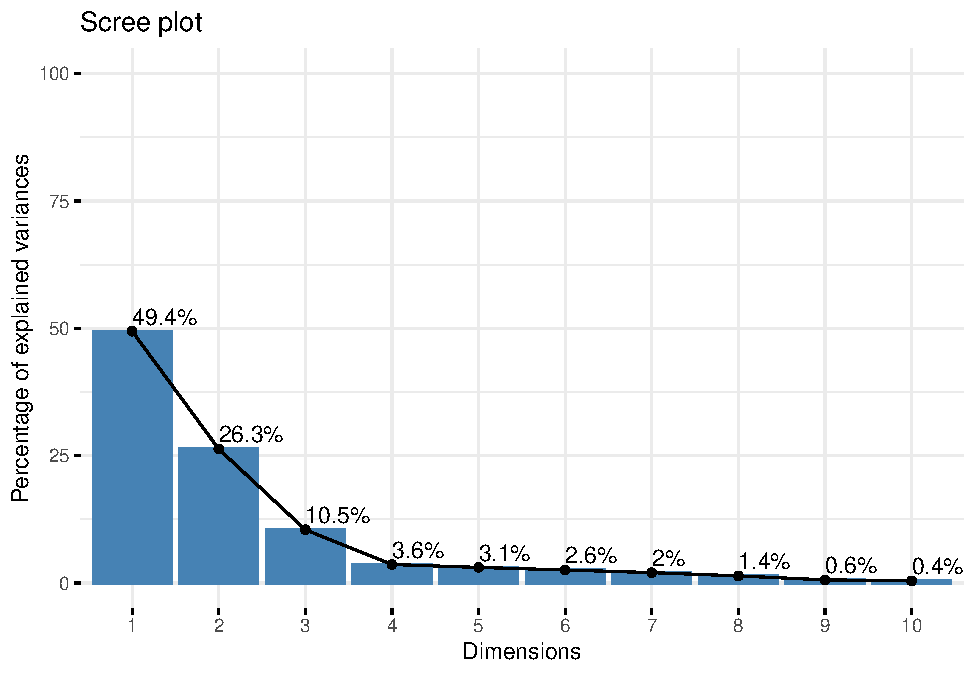
\includegraphics{rEkonometri_files/figure-latex/unnamed-chunk-92-1.pdf}

Mesela burada ilk altısı bizi tatmin ediyor. Çünkü kümülatife baktığımızda \%95.5'ini açıklıyor. Bu durumda kalan dördünü atabiliriz.

İlk altı özvektörü kullanalım. Standardize edilmiş veri seti ile skorları (ilk altısı) çarpıp yeni bir matris elde edeceğiz.

\begin{Shaded}
\begin{Highlighting}[]
\NormalTok{pcr <-}\StringTok{ }\KeywordTok{princomp}\NormalTok{(df1_yeni[,}\OperatorTok{-}\DecValTok{11}\NormalTok{])}
\NormalTok{df_ <-}\StringTok{ }\KeywordTok{lm}\NormalTok{(df1_yeni}\OperatorTok{$}\NormalTok{y }\OperatorTok{~}\StringTok{ }\DecValTok{0} \OperatorTok{+}\StringTok{ }\NormalTok{pcr}\OperatorTok{$}\NormalTok{scores[,}\DecValTok{1}\NormalTok{] }\OperatorTok{+}\StringTok{ }\NormalTok{pcr}\OperatorTok{$}\NormalTok{scores[,}\DecValTok{2}\NormalTok{] }\OperatorTok{+}\StringTok{ }\NormalTok{pcr}\OperatorTok{$}\NormalTok{scores[,}\DecValTok{3}\NormalTok{] }\OperatorTok{+}\StringTok{ }\NormalTok{pcr}\OperatorTok{$}\NormalTok{scores[,}\DecValTok{4}\NormalTok{] }\OperatorTok{+}\StringTok{ }\NormalTok{pcr}\OperatorTok{$}\NormalTok{scores[,}\DecValTok{5}\NormalTok{] }\OperatorTok{+}\StringTok{ }\NormalTok{pcr}\OperatorTok{$}\NormalTok{scores[,}\DecValTok{6}\NormalTok{])}
\KeywordTok{summary}\NormalTok{(df_)}
\end{Highlighting}
\end{Shaded}

\begin{verbatim}
## 
## Call:
## lm(formula = df1_yeni$y ~ 0 + pcr$scores[, 1] + pcr$scores[, 
##     2] + pcr$scores[, 3] + pcr$scores[, 4] + pcr$scores[, 5] + 
##     pcr$scores[, 6])
## 
## Residuals:
##     Min      1Q  Median      3Q     Max 
## -91.680 -50.984  -8.005  45.460 133.215 
## 
## Coefficients:
##                 Estimate Std. Error t value Pr(>|t|)    
## pcr$scores[, 1]  192.162      8.041  23.896 3.98e-12 ***
## pcr$scores[, 2]  -13.275     11.024  -1.204   0.2500    
## pcr$scores[, 3]  -33.127     17.475  -1.896   0.0805 .  
## pcr$scores[, 4]  -73.941     29.637  -2.495   0.0268 *  
## pcr$scores[, 5]  -64.063     32.277  -1.985   0.0687 .  
## pcr$scores[, 6]   15.674     35.310   0.444   0.6644    
## ---
## Signif. codes:  0 '***' 0.001 '**' 0.01 '*' 0.05 '.' 0.1 ' ' 1
## 
## Residual standard error: 75.87 on 13 degrees of freedom
## Multiple R-squared:  0.9783, Adjusted R-squared:  0.9683 
## F-statistic: 97.74 on 6 and 13 DF,  p-value: 4.701e-10
\end{verbatim}

Bu sonuçlardan bağımlı değişken Y'yi en iyi PC1 ile PC4'ün açıkladığını söyleyebiliriz. Gujarati şöyle der: \emph{Kuşkusuz buradaki güçlük bu temel bileşenleri nasıl yorumlamamız gerektiğini bilmiyor olmamızdandır. Ancak temel bileşenler yöntemi korelasyonlu açıklayıcı değişken sayısını korelasyonsuz birkaç değişkene indirgemede kullanışlı bir yoldur. Sonuç olarak doğrusal bağlantı sorunuyla karşılaşmayız.}

\hypertarget{ridge-regresyon}{%
\section{Ridge Regresyon}\label{ridge-regresyon}}

Bu konuyu, \emph{Yumurta tavukçuluğunda gelirin Ridge Regresyon analizi ile tahmini} çalışmasından faydalanarak inceleyeceğiz.

\begin{Shaded}
\begin{Highlighting}[]
\NormalTok{df2}\OperatorTok{$}\NormalTok{yas_hafta <-}\StringTok{ }\OtherTok{NULL} \CommentTok{#Buradaki yaş, ay ile ilgilidir. O nedenle hafta sütunu atıldı.}
\KeywordTok{head}\NormalTok{(df2, }\DecValTok{10}\NormalTok{)}
\end{Highlighting}
\end{Shaded}

\begin{verbatim}
##    yas_ay yasama_gucu yumurta_verimi yumurta_agirligi gelir
## 1       1        99.9            1.0             43.0    78
## 2       1        99.8           11.0             44.4   839
## 3       1        99.7           35.0             45.4  3257
## 4       1        99.6           53.0             47.9  4927
## 5       2        99.5           77.0             49.1  7061
## 6       2        99.4           91.0             50.4 10078
## 7       2        99.3           92.0             52.5  9779
## 8       2        99.2           93.0             53.6  9929
## 9       3        99.1           94.0             54.6 10080
## 10      3        99.0           94.5             55.4 10587
\end{verbatim}

Bağımlı değişken:

\begin{itemize}
\tightlist
\item
  \textbf{gelir}
\end{itemize}

Bağımsız değişken(ler):

\begin{itemize}
\item
  \textbf{yasama\_gucu}
\item
  \textbf{yumurta\_verimi}
\item
  \textbf{yumurta\_agirligi}
\item
  \textbf{yas\_ay}
\end{itemize}

Ridge regresyon bir sapmalı tahmin yöntemidir. Sapmalı tahmin yöntemi, parametrelerde gerçekleşmesi beklenen sonuçlara ulaşmayı ve bu sonuçlara ulaşırken varyansların küçülmesini sağlar.

Kısa bir hatırlatma:

Matrisler ile parametre tahminini \(\hat{\beta} = (X'X)^{-1} (X'Y)\) eşitliği ile buluyorduk.

Çoklu doğrusal bağlantı sözkonusu olduğunda \((X'X)^{-1}\) matrisinin köşegen elemanları çok büyük değerler almaktadır. Bu sorunu giderebilmek için \(X'X\) matrisinin köşegen elemanlarına bir sabitin eklenmesi ile \((X'X + kI)^{-1}\) şeklinde ridge tahmincisi oluşturulmuş olur. Bu sabit k'dır. Bu değer seçilirken \(\frac{1}{n}\sum (Y_i - \hat{Y_i})^2\) ile bulunan ortalama hata kareyi azaltmaya ve sapmayı mümkün olduğunca küçük tutmaya dikkat edilmelidir. 0-1 arasında değer alan k'nın 0'a yakın olması istenir. Eğer 0 olursa Sıradan En Küçük Kareler tahminleri ile aynı olur.

Önce bildiğimiz haliyle regresyon modelini kuralım.

\begin{Shaded}
\begin{Highlighting}[]
\NormalTok{model1 <-}\StringTok{ }\KeywordTok{lm}\NormalTok{(}\DataTypeTok{formula =}\NormalTok{ gelir }\OperatorTok{~}\StringTok{ }\NormalTok{yasama_gucu }\OperatorTok{+}\StringTok{ }\NormalTok{yumurta_verimi }\OperatorTok{+}\StringTok{ }\NormalTok{yumurta_agirligi }\OperatorTok{+}\StringTok{ }\NormalTok{yas_ay, }\DataTypeTok{data =}\NormalTok{ df2)}
\KeywordTok{summary}\NormalTok{(model1) }\CommentTok{#Verileri defalarca kez kontrol etmeme rağmen çalışma ile aynı çıktıyı alamadım. İşaretlerde bir problem yok.}
\end{Highlighting}
\end{Shaded}

\begin{verbatim}
## 
## Call:
## lm(formula = gelir ~ yasama_gucu + yumurta_verimi + yumurta_agirligi + 
##     yas_ay, data = df2)
## 
## Residuals:
##     Min      1Q  Median      3Q     Max 
## -870.50 -131.17    1.62  116.92  602.18 
## 
## Coefficients:
##                   Estimate Std. Error t value Pr(>|t|)    
## (Intercept)      24655.490  28766.223   0.857   0.3949    
## yasama_gucu       -270.874    285.774  -0.948   0.3471    
## yumurta_verimi     103.992      3.634  28.616   <2e-16 ***
## yumurta_agirligi    47.181     20.534   2.298   0.0252 *  
## yas_ay             -47.987    112.979  -0.425   0.6726    
## ---
## Signif. codes:  0 '***' 0.001 '**' 0.01 '*' 0.05 '.' 0.1 ' ' 1
## 
## Residual standard error: 248 on 58 degrees of freedom
## Multiple R-squared:  0.9857, Adjusted R-squared:  0.9848 
## F-statistic:  1002 on 4 and 58 DF,  p-value: < 2.2e-16
\end{verbatim}

Değişkenler arası korelasyonlar:

\begin{Shaded}
\begin{Highlighting}[]
\KeywordTok{corrplot}\NormalTok{(}\KeywordTok{cor}\NormalTok{(df2[,}\OperatorTok{-}\DecValTok{1}\NormalTok{]), }\DataTypeTok{method =} \StringTok{"number"}\NormalTok{, }\DataTypeTok{type =} \StringTok{"lower"}\NormalTok{)}
\end{Highlighting}
\end{Shaded}

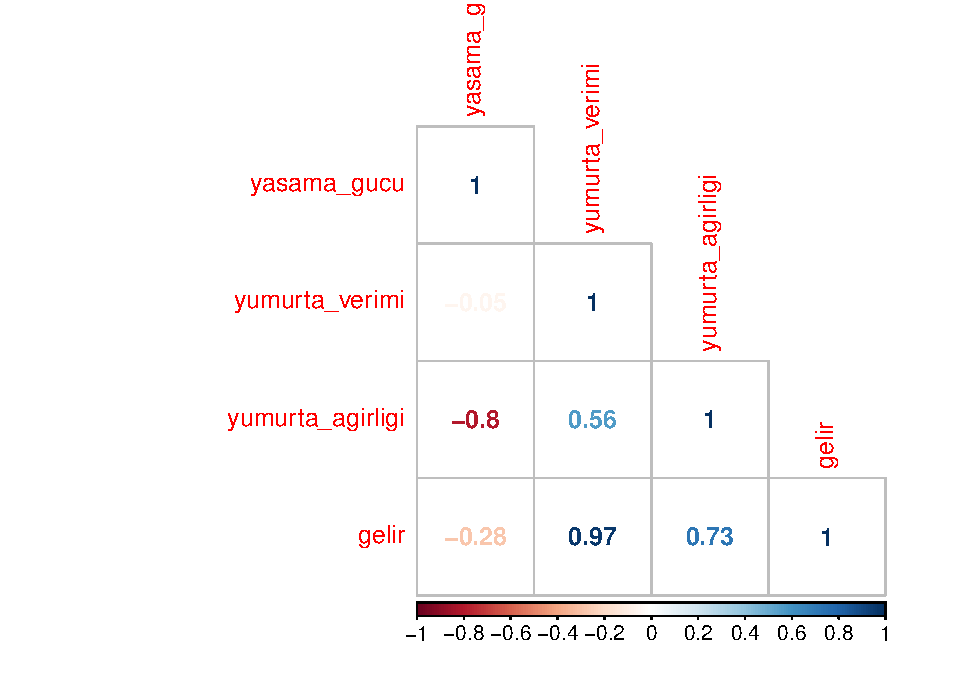
\includegraphics{rEkonometri_files/figure-latex/unnamed-chunk-96-1.pdf}

Yüksek \(R^2\), güçlü korelasyonlar ve istatistiksel olarak anlamlı olmayan parametreler elde ettik.

VIF değerleri ise aşağıdaki gibidir:

\begin{Shaded}
\begin{Highlighting}[]
\NormalTok{car}\OperatorTok{::}\KeywordTok{vif}\NormalTok{(model1)}
\end{Highlighting}
\end{Shaded}

\begin{verbatim}
##      yasama_gucu   yumurta_verimi yumurta_agirligi           yas_ay 
##       276.549977         3.943549        10.769081       270.325334
\end{verbatim}

Yumurta verimi dışındaki değişkenlerin \textgreater10 olduğunu görüyoruz.

Aslında çoklu doğrusal bağlantının sinyallerini almış olduk.

Modeli kurmadan önce ridge izi kavramını bilmemiz gerekiyor. Ridge regresyon yönteminde en önemli nokta olan k değerinin seçimi için çeşitli yol ve algoritmalar geliştirilmiştir. Bunlardan biri ridge izidir. Burada amaç çoklu doğrusal bağlantının etkilerini görerek uygun k değerinin seçilmesidir.

Ridge regresyon modelini kuralım. Ardından hem ridge hem de VIF grafiklerine bakalım.

\begin{Shaded}
\begin{Highlighting}[]
\NormalTok{model2 <-}\StringTok{ }\KeywordTok{lmridge}\NormalTok{(}\DataTypeTok{formula =}\NormalTok{ gelir }\OperatorTok{~}\NormalTok{., }\DataTypeTok{data =}\NormalTok{ df2, }\DataTypeTok{K =} \KeywordTok{seq}\NormalTok{(}\DecValTok{0}\NormalTok{, }\FloatTok{0.1}\NormalTok{, }\FloatTok{0.01}\NormalTok{))}

\KeywordTok{seq}\NormalTok{(}\DecValTok{0}\NormalTok{, }\FloatTok{0.1}\NormalTok{, }\FloatTok{0.01}\NormalTok{) }\CommentTok{#En uygun k, şunlardan biri olacak.}
\end{Highlighting}
\end{Shaded}

\begin{verbatim}
##  [1] 0.00 0.01 0.02 0.03 0.04 0.05 0.06 0.07 0.08 0.09 0.10
\end{verbatim}

Aşağıdaki ridge izi grafiğinde çok küçük bir k değerinden sonra parametrelerin yataylaştığını gözlemliyoruz.

\begin{Shaded}
\begin{Highlighting}[]
\KeywordTok{plot}\NormalTok{(model2, }\DataTypeTok{type =} \StringTok{"ridge"}\NormalTok{)}
\end{Highlighting}
\end{Shaded}

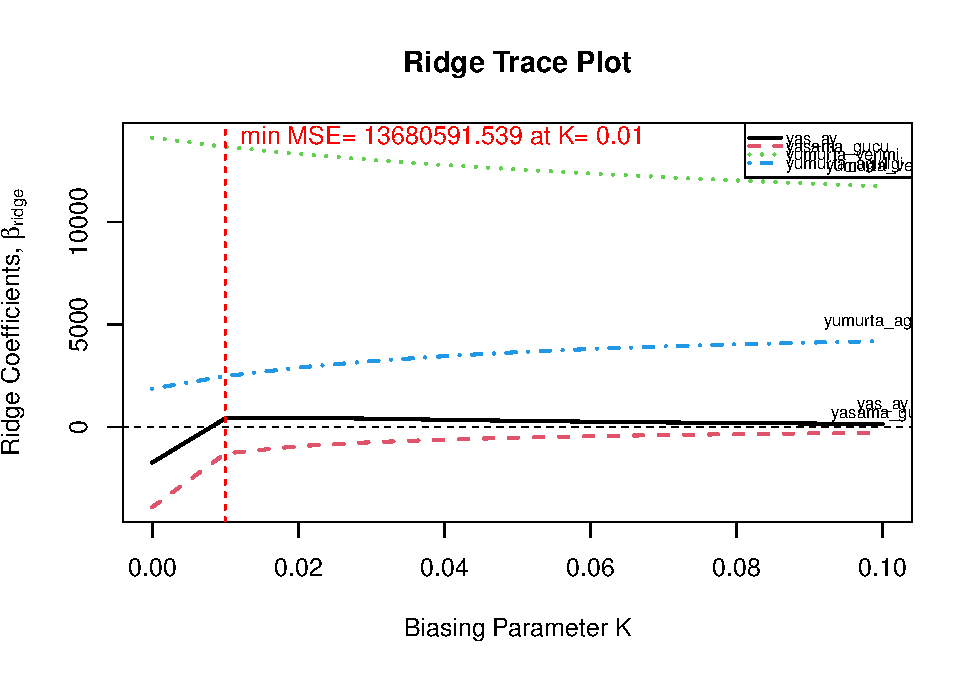
\includegraphics{rEkonometri_files/figure-latex/unnamed-chunk-99-1.pdf}

Aşağıdaki VIF grafiğinde ise yine aynı k değerinden sonra değerler 10 sınırının altına iniyor.

\begin{Shaded}
\begin{Highlighting}[]
\KeywordTok{plot}\NormalTok{(model2, }\DataTypeTok{type =} \StringTok{"vif"}\NormalTok{)}
\end{Highlighting}
\end{Shaded}

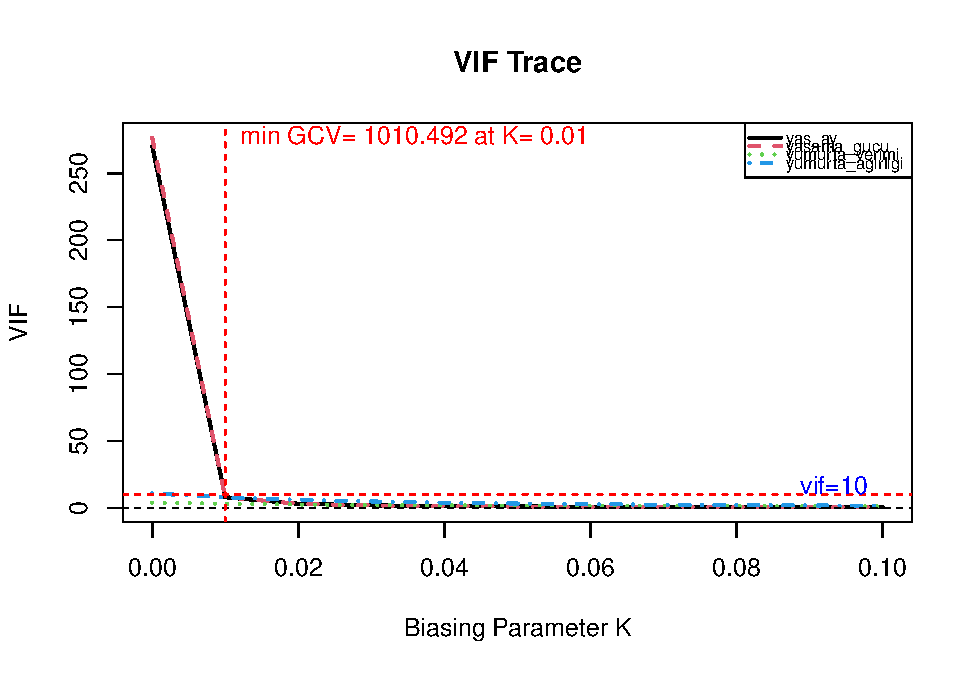
\includegraphics{rEkonometri_files/figure-latex/unnamed-chunk-100-1.pdf}

Çalışmada da olduğu gibi en uygun k değerini 0.01 olarak bulduk. k = 0.01'e ait parametreler (2. sıra) şöyledir:

\begin{Shaded}
\begin{Highlighting}[]
\KeywordTok{coef}\NormalTok{(model2)}
\end{Highlighting}
\end{Shaded}

\begin{verbatim}
##         Intercept    yas_ay yasama_gucu yumurta_verimi yumurta_agirligi
## K=0    24655.4905 -47.98664  -270.87431      103.99232         47.18072
## K=0.01  5941.3695  11.59113   -89.39626      100.73553         62.46986
## K=0.02  3112.2073  12.59763   -64.61345       98.16766         73.03809
## K=0.03  1539.2932  11.25819   -51.35461       96.03373         80.98819
## K=0.04   473.4126   9.72173   -42.46333       94.20393         87.14092
## K=0.05  -302.4989   8.33787   -35.97024       92.59687         92.00060
## K=0.06  -887.3391   7.16174   -31.01780       91.15870         95.89881
## K=0.07 -1336.6124   6.18190   -27.14084       89.85224         99.06321
## K=0.08 -1685.2260   5.37242   -24.05395       88.65103        101.65538
## K=0.09 -1956.7308   4.70682   -21.56798       87.53565        103.79320
## K=0.1  -2167.7917   4.16175   -19.55083       86.49155        105.56471
\end{verbatim}

k = 0 iken parametrelerin önceki model ile aynı olduğuna dikkat edin. \emph{Eğer 0 olursa Sıradan En Küçük Kareler tahminleri ile aynı olur} demiştik.

Modeli k = 0.01 ile yeniden kuralım.

\begin{Shaded}
\begin{Highlighting}[]
\NormalTok{model2 <-}\StringTok{ }\KeywordTok{lmridge}\NormalTok{(}\DataTypeTok{formula =}\NormalTok{ gelir }\OperatorTok{~}\StringTok{ }\NormalTok{., }\DataTypeTok{data =}\NormalTok{ df2, }\DataTypeTok{K =} \FloatTok{0.01}\NormalTok{)}
\KeywordTok{summary}\NormalTok{(model2)}
\end{Highlighting}
\end{Shaded}

\begin{verbatim}
## 
## Call:
## lmridge.default(formula = gelir ~ ., data = df2, K = 0.01)
## 
## 
## Coefficients: for Ridge parameter K= 0.01 
##                     Estimate Estimate (Sc) StdErr (Sc) t-value (Sc) Pr(>|t|)
## Intercept         5.9414e+03   -1.1371e+06  8.6849e+04     -13.0931   <2e-16
## yas_ay            1.1591e+01    4.1838e+02  6.9544e+02       0.6016   0.5497
## yasama_gucu      -8.9396e+01   -1.2903e+03  6.9652e+02      -1.8525   0.0690
## yumurta_verimi    1.0074e+02    1.3653e+04  4.3104e+02      31.6751   <2e-16
## yumurta_agirligi  6.2470e+01    2.4762e+03  6.9175e+02       3.5796   0.0007
##                     
## Intercept        ***
## yas_ay              
## yasama_gucu      .  
## yumurta_verimi   ***
## yumurta_agirligi ***
## ---
## Signif. codes:  0 '***' 0.001 '**' 0.01 '*' 0.05 '.' 0.1 ' ' 1
## 
## Ridge Summary
##         R2     adj-R2   DF ridge          F        AIC        BIC 
##    0.96990    0.96840    2.99721 1012.09783  696.71631  964.15722 
## Ridge minimum MSE= 13680592 at K= 0.01 
## P-value for F-test ( 2.99721 , 59.73467 ) = 3.901713e-51 
## -------------------------------------------------------------------
\end{verbatim}

Çalışmanın sonuç bölümünden:

\emph{Sonuç olarak, bu çalışmada yumurta tavukçuluğunda satış gelirini etkileyebilecek değişkenler arasında, güçlü çoklu doğrusal bağlantı yapısından, RR (Ridge Regresyon) yönteminin EKK (En Küçük Kareler) yöntemine göre daha geçerli, tutarlı, durağan ve beklentilere uygun tahminler sağladığı görülmüştür. Çoklu regresyon analizinde eğer çoklu doğrusal bağlantı söz konusu ise, EKK yöntemiyle parametre tahmininde bulunmak yanlış sonuçlar alınmasına ve yorumlanmasına neden olabilir.}

\hypertarget{deux11fiux15fen-varyans}{%
\chapter{Değişen Varyans}\label{deux11fiux15fen-varyans}}

Regresyon modelindeki hata terimi gözlemler boyunca sabit varyanslıdır (homoscedasticity). Sabit varyans olmaması durumu ise değişen varyanstır (heteroscedasticity). Burada bir noktanın altını çizmek gerekiyor: Bu varsayım, her bir gözlemin varyansının aynı olmasını ifade eder; örnek gözlemlerinin tümü için varyansın sabit olmasını değil. Bunu Stock ve Watson'ın kitabında bulunan bir örnek ile açıklayalım.

\begin{Shaded}
\begin{Highlighting}[]
\KeywordTok{library}\NormalTok{(AER);}\KeywordTok{library}\NormalTok{(ggplot2)}
\KeywordTok{data}\NormalTok{(}\StringTok{"CPSSWEducation"}\NormalTok{) }\CommentTok{#Kitaptaki verilere AER paketi yardımı ile ulaşılabilir.}
\KeywordTok{head}\NormalTok{(CPSSWEducation, }\DecValTok{10}\NormalTok{)}
\end{Highlighting}
\end{Shaded}

\begin{verbatim}
##    age gender  earnings education
## 1   30   male 34.615383        16
## 2   30 female 19.230770        16
## 3   30 female 13.736263        12
## 4   30 female 13.942307        13
## 5   30 female 19.230770        16
## 6   30 female  8.000000        12
## 7   30   male 19.230770        12
## 8   29   male 26.153847        16
## 9   29   male 26.442308        16
## 10  30 female  6.221719        12
\end{verbatim}

\begin{Shaded}
\begin{Highlighting}[]
\KeywordTok{ggplot}\NormalTok{(}\DataTypeTok{data =}\NormalTok{ CPSSWEducation, }\KeywordTok{aes}\NormalTok{(}\DataTypeTok{x =}\NormalTok{ education, }\DataTypeTok{y =}\NormalTok{ earnings)) }\OperatorTok{+}
\StringTok{  }\KeywordTok{geom_point}\NormalTok{() }\OperatorTok{+}
\StringTok{  }\KeywordTok{geom_smooth}\NormalTok{(}\DataTypeTok{method =} \StringTok{"lm"}\NormalTok{, }\DataTypeTok{se =} \OtherTok{FALSE}\NormalTok{, }\DataTypeTok{color =} \StringTok{"red"}\NormalTok{) }\OperatorTok{+}
\StringTok{  }\KeywordTok{theme_minimal}\NormalTok{()}
\end{Highlighting}
\end{Shaded}

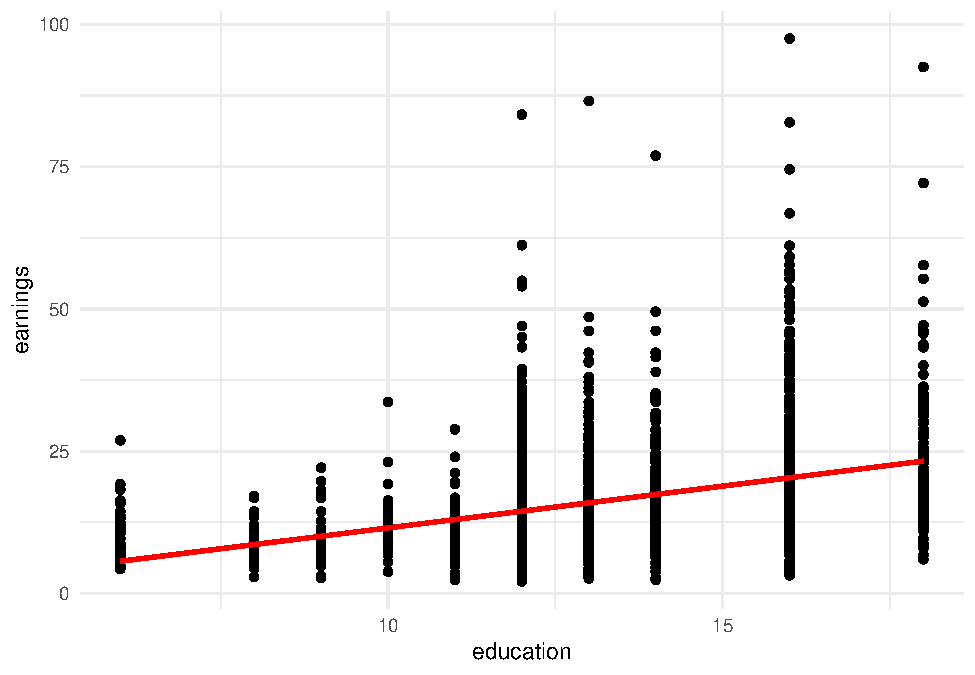
\includegraphics{rEkonometri_files/figure-latex/unnamed-chunk-103-1.pdf}

Eğitim düzeyi daha yüksek olan çalışanların eğitim düzeyi daha düşük olan çalışanlara göre kazançları (earnings) ortalama olarak daha fazladır. Ancak kazancı daha yüksek olan işler eğitim düzeyi daha yüksek olan kişiler tarafından alınıyorsa kazançların dağılımının \emph{varyansı} eğitim düzeyi yüksek olan çalışanlar için daha büyük olabilir.

Şimdi bir model kuralım.

Bağımlı değişken:

\begin{itemize}
\tightlist
\item
  \textbf{earnings:} Saatlik kazanç
\end{itemize}

Bağımsız değişken(ler):

\begin{itemize}
\tightlist
\item
  \textbf{education:} Eğitim düzeyi (6-18 yıl arasında değişen)
\end{itemize}

\begin{Shaded}
\begin{Highlighting}[]
\NormalTok{model <-}\StringTok{ }\KeywordTok{lm}\NormalTok{(}\DataTypeTok{formula =}\NormalTok{ earnings }\OperatorTok{~}\StringTok{ }\NormalTok{education, }\DataTypeTok{data =}\NormalTok{ CPSSWEducation)}
\KeywordTok{summary}\NormalTok{(model)}
\end{Highlighting}
\end{Shaded}

\begin{verbatim}
## 
## Call:
## lm(formula = earnings ~ education, data = CPSSWEducation)
## 
## Residuals:
##     Min      1Q  Median      3Q     Max 
## -17.270  -5.355  -1.513   3.194  77.164 
## 
## Coefficients:
##             Estimate Std. Error t value Pr(>|t|)    
## (Intercept) -3.13437    0.95925  -3.268   0.0011 ** 
## education    1.46693    0.06978  21.021   <2e-16 ***
## ---
## Signif. codes:  0 '***' 0.001 '**' 0.01 '*' 0.05 '.' 0.1 ' ' 1
## 
## Residual standard error: 8.769 on 2948 degrees of freedom
## Multiple R-squared:  0.1304, Adjusted R-squared:  0.1301 
## F-statistic: 441.9 on 1 and 2948 DF,  p-value: < 2.2e-16
\end{verbatim}

Ortalama olarak saatlik kazanç her bir ilave eğitim yılı için 1.47 \$ artmaktadır. Güven aralığı \%95 güven düzeyinde aşağıdaki gibidir:

\begin{Shaded}
\begin{Highlighting}[]
\KeywordTok{confint}\NormalTok{(model, }\DataTypeTok{level =} \FloatTok{0.95}\NormalTok{)}
\end{Highlighting}
\end{Shaded}

\begin{verbatim}
##                 2.5 %    97.5 %
## (Intercept) -5.015248 -1.253495
## education    1.330098  1.603753
\end{verbatim}

Standart sapma değerleri yıl olarak eğitim düzeyine göre farklılaştığı için regresyon modeline ilişkin kalıntıların varyansı bağımsız değişkene (yıl olarak eğitim düzeyi) bağlıdır. Yani, değişen varyans söz konusudur.

\begin{Shaded}
\begin{Highlighting}[]
\KeywordTok{library}\NormalTok{(dplyr)}

\NormalTok{CPSSWEducation }\OperatorTok\StringTok{ }
\StringTok{  }\KeywordTok{group_by}\NormalTok{(education) }\OperatorTok\StringTok{ }
\StringTok{  }\KeywordTok{summarise}\NormalTok{(}\DataTypeTok{ss =} \KeywordTok{round}\NormalTok{(}\KeywordTok{sd}\NormalTok{(earnings), }\DataTypeTok{digits =} \DecValTok{2}\NormalTok{)) }\CommentTok{#Standart sapmalar alındı.}
\end{Highlighting}
\end{Shaded}

\begin{verbatim}
## # A tibble: 10 x 2
##    education    ss
##        <int> <dbl>
##  1         6  4.48
##  2         8  3.53
##  3         9  4.26
##  4        10  5.46
##  5        11  5.13
##  6        12  7.43
##  7        13  8.05
##  8        14  8.23
##  9        16 10.8 
## 10        18 11.8
\end{verbatim}

Değişen varyansın nedenleri aşağıdaki gibi sıralanabilir.

\begin{itemize}
\item
  Hatasını öğrenen modellerde, tıpkı insanların öğrenmesi gibi davranış hataları zamanla azalır ya da hata sayıları daha tutarlı hale gelir.
\item
  Örneğin, gelir yükseldikçe insanların istedikleri gibi harcayabilecekleri gelir daha çok olur, seçenekler gelişir (varyans artırıcı etki) ya da daha çok kar eden şirketlerin temettü dağıtımlarında düşük karlı şirketlere göre genellikle daha çok değişkenlik göstermesi beklenir (varyans artırıcı etki).
\item
  Verilerin toplanmasında bazı hatalar yapılabilir. Veri derleme teknikleri geliştikçe (daha az hataların ortaya çıkması) varyans da düşebilir.
\item
  Aykırı/uç değerlerin varlığı.
\item
  Model kurma hataları.
\item
  Modelde yer alan değişkenlerin birinde ya da birkaçında bulunan çarpıklık.
\item
  Yanlış veri dönüştürmeleri ya da yanlış fonksiyon kalıbı.
\end{itemize}

Değişen varyans varsa neler olur?

\begin{itemize}
\item
  Sıradan En Küçük Kareler tahmincileri için BLUE'dur (Best Linear Unbiased Estimator, En İyi Doğrusal Yansız Tahmin Edici) demiştik. Değişen varyans olması durumunda doğrusal yansız tahmin edici olur.
\item
  t ve F testlerine olan güven azalır.
\item
  Değişen varyans durumunda BLUE tahmincilerini ağırlıklı en küçük kareler yöntemi verir.
\end{itemize}

Değişen varyans durumunun tespiti konusunda iki testten yararlanacağız: Breusch-Pagan ve White testleri.

Ne tür düzeltici önlemler alabiliriz?

\begin{enumerate}
\def\labelenumi{\roman{enumi}.}
\item
  Eğer gerçek hata terimi varyansı bağımsız değişkenlerden birinin karesi ile orantılı ise eşitliğin her iki tarafı bu değişkene bölünüp regresyon çalıştırabilir. Ardından bunları Breusch-Pagan ve White testlerinden geçirebiliriz.
\item
  Eğer gerçek hata terimi varyansı bağımsız değişkenlerden birisi ile orantılıysa karekök dönüşümü kullanılabilir. Yani, her iki taraf belirlenen bağımsız değişkenin kareköküne bölünür. Ardından Breusch-Pagan ve White testlerinden geçirebiliriz.
\item
  Eğer değerler pozitifse bağımlı değişkenin logaritması alınabilir.
\end{enumerate}

\begin{Shaded}
\begin{Highlighting}[]
\KeywordTok{library}\NormalTok{(readxl);}\KeywordTok{library}\NormalTok{(tidyverse);}\KeywordTok{library}\NormalTok{(magrittr);}\KeywordTok{library}\NormalTok{(lmtest);}\KeywordTok{library}\NormalTok{(estimatr)}
\end{Highlighting}
\end{Shaded}

\begin{Shaded}
\begin{Highlighting}[]
\KeywordTok{setwd}\NormalTok{(}\StringTok{"C:/Users/datanerd/Desktop/Github/rEkonometri/data"}\NormalTok{)}
\NormalTok{df <-}\StringTok{ }\KeywordTok{read_excel}\NormalTok{(}\StringTok{"Table1_1.xls"}\NormalTok{)}
\NormalTok{df }\OperatorTok\StringTok{ }
\StringTok{  }\NormalTok{dplyr}\OperatorTok{::}\KeywordTok{select}\NormalTok{(wage, female, nonwhite, union, education, exper)}
\end{Highlighting}
\end{Shaded}

\hypertarget{breusch-pagan}{%
\section{Breusch-Pagan}\label{breusch-pagan}}

Büyük örneklemler içindir. Sıradan En Küçük Kareler regresyonu tahmin edilip bu regresyondan kalıntı kareleri elde edilir. Ardından kalıntı karelerin bir veya daha fazla X değişkeni ile ilişkili olup olmadığını görmek için kalıntı karelerin modele dahil edilen bağımsız değişkenlere göre regresyonu alınır. Buradaki \(H_0\) hata teriminin sabit varyanslı olduğudur. Bu hipotezin testi için F testini (pay ve payda sırasıyla k-1 ve n-k serbestlik dereceli olacak) kullanabiliriz. F istatistiği istatistiksel olarak anlamlı ise \(H_0\) reddedilir. F istatistiğine alternatif olarak \(\chi^2\) istatistiği de kullanılabilir. \(\chi^2\) değeri küçük bir p değerine sahipse \(H_0\) reddedilebilir.

Öncelikle modeli normal bir şekilde kuralım.

\begin{Shaded}
\begin{Highlighting}[]
\NormalTok{model <-}\StringTok{ }\KeywordTok{lm}\NormalTok{(}\DataTypeTok{formula =}\NormalTok{ wage }\OperatorTok{~}\StringTok{ }\NormalTok{female }\OperatorTok{+}\StringTok{ }\NormalTok{nonwhite }\OperatorTok{+}\StringTok{ }\NormalTok{union }\OperatorTok{+}\StringTok{ }\NormalTok{education }\OperatorTok{+}\StringTok{ }\NormalTok{exper, }\DataTypeTok{data =}\NormalTok{ df)}
\KeywordTok{summary}\NormalTok{(model)}
\end{Highlighting}
\end{Shaded}

\begin{verbatim}
## 
## Call:
## lm(formula = wage ~ female + nonwhite + union + education + exper, 
##     data = df)
## 
## Residuals:
##     Min      1Q  Median      3Q     Max 
## -20.781  -3.760  -1.044   2.418  50.414 
## 
## Coefficients:
##             Estimate Std. Error t value Pr(>|t|)    
## (Intercept) -7.18334    1.01579  -7.072 2.51e-12 ***
## female      -3.07488    0.36462  -8.433  < 2e-16 ***
## nonwhite    -1.56531    0.50919  -3.074  0.00216 ** 
## union        1.09598    0.50608   2.166  0.03052 *  
## education    1.37030    0.06590  20.792  < 2e-16 ***
## exper        0.16661    0.01605  10.382  < 2e-16 ***
## ---
## Signif. codes:  0 '***' 0.001 '**' 0.01 '*' 0.05 '.' 0.1 ' ' 1
## 
## Residual standard error: 6.508 on 1283 degrees of freedom
## Multiple R-squared:  0.3233, Adjusted R-squared:  0.3207 
## F-statistic: 122.6 on 5 and 1283 DF,  p-value: < 2.2e-16
\end{verbatim}

Ardından bu modelden kalıntı kareleri elde edip bir model daha kuralım.

\begin{Shaded}
\begin{Highlighting}[]
\NormalTok{df}\OperatorTok{$}\NormalTok{res <-}\StringTok{ }\NormalTok{(model}\OperatorTok{$}\NormalTok{residuals)}\OperatorTok{^}\DecValTok{2}
\NormalTok{modelres <-}\StringTok{ }\KeywordTok{lm}\NormalTok{(res }\OperatorTok{~}\StringTok{ }\NormalTok{female }\OperatorTok{+}\StringTok{ }\NormalTok{nonwhite }\OperatorTok{+}\StringTok{ }\NormalTok{union }\OperatorTok{+}\StringTok{ }\NormalTok{education }\OperatorTok{+}\StringTok{ }\NormalTok{exper, }\DataTypeTok{data =}\NormalTok{ df)}
\KeywordTok{summary}\NormalTok{(modelres)}
\end{Highlighting}
\end{Shaded}

\begin{verbatim}
## 
## Call:
## lm(formula = res ~ female + nonwhite + union + education + exper, 
##     data = df)
## 
## Residuals:
##     Min      1Q  Median      3Q     Max 
## -110.57  -36.73  -18.33   -1.47 2483.23 
## 
## Coefficients:
##             Estimate Std. Error t value Pr(>|t|)    
## (Intercept) -73.3377    19.6801  -3.726 0.000203 ***
## female       -9.7007     7.0642  -1.373 0.169924    
## nonwhite    -12.6683     9.8651  -1.284 0.199321    
## union       -27.2099     9.8049  -2.775 0.005598 ** 
## education     7.9624     1.2768   6.236 6.08e-10 ***
## exper         1.1665     0.3109   3.752 0.000183 ***
## ---
## Signif. codes:  0 '***' 0.001 '**' 0.01 '*' 0.05 '.' 0.1 ' ' 1
## 
## Residual standard error: 126.1 on 1283 degrees of freedom
## Multiple R-squared:  0.04292,    Adjusted R-squared:  0.03919 
## F-statistic: 11.51 on 5 and 1283 DF,  p-value: 6.878e-11
\end{verbatim}

\%4.3 olan bir \(R^2\) elde ettik. Bu değeri gözlem sayısı olan 1289 ile çarpıp aşağıdaki \(\chi^2\) değerini elde ederiz.

\begin{Shaded}
\begin{Highlighting}[]
\KeywordTok{summary}\NormalTok{(modelres)}\OperatorTok{$}\NormalTok{r.squared }\OperatorTok{*}\StringTok{ }\KeywordTok{nrow}\NormalTok{(df)}
\end{Highlighting}
\end{Shaded}

\begin{verbatim}
## [1] 55.32705
\end{verbatim}

Tabi bunu paket yardımı ile de yapabiliriz. Hatta buradan p değerini de elde edip hipotezin red olup olmayacağına karar vereceğiz.

\begin{Shaded}
\begin{Highlighting}[]
\KeywordTok{bptest}\NormalTok{(model)}
\end{Highlighting}
\end{Shaded}

\begin{verbatim}
## 
##  studentized Breusch-Pagan test
## 
## data:  model
## BP = 55.327, df = 5, p-value = 1.118e-10
\end{verbatim}

5 serbestlik dereceli (bağımsız değişken sayımız) en az bu değerde bir \(\chi^2\) bulma olasılığı neredeyse sıfırdır (0.0000000001118). Yani, \(H_0\) reddedilir. Bu da değişen varyansa işaret ediyor.

\hypertarget{white}{%
\section{White}\label{white}}

Büyük örneklemler içindir. Yukarıdaki teste göre daha genel ve daha esnektir. Burada da \(\chi^2\) istatistiği kullanılabilir. White testinin uygulanması için kurulan model tahmin edilerek kalıntılar belirlenir. Belirlenen kalıntıların karelerinin bağımlı değişken olduğu, bağımsız değişkenlerin ise modelin bağımsız değişkenleri, bağımsız değişkenlerin kareleri ve bağımsız değişkenlerin birbirleri ile çarpımlarından oluşan yardımcı regresyon modeli tahmin edilir.

\begin{Shaded}
\begin{Highlighting}[]
\NormalTok{model <-}\StringTok{ }\KeywordTok{lm}\NormalTok{(}\DataTypeTok{formula =}\NormalTok{ wage }\OperatorTok{~}\StringTok{ }\NormalTok{female }\OperatorTok{+}\StringTok{ }\NormalTok{nonwhite }\OperatorTok{+}\StringTok{ }\NormalTok{union }\OperatorTok{+}\StringTok{ }\NormalTok{education }\OperatorTok{+}\StringTok{ }\NormalTok{exper, }\DataTypeTok{data =}\NormalTok{ df)}
\KeywordTok{bptest}\NormalTok{(model, }\OperatorTok{~}\StringTok{ }\NormalTok{female}\OperatorTok{*}\NormalTok{nonwhite }\OperatorTok{+}\StringTok{ }\NormalTok{female}\OperatorTok{*}\NormalTok{union }\OperatorTok{+}\StringTok{ }\NormalTok{female}\OperatorTok{*}\NormalTok{education }\OperatorTok{+}\StringTok{ }\NormalTok{female}\OperatorTok{*}\NormalTok{exper }\OperatorTok{+}\StringTok{ }\NormalTok{nonwhite}\OperatorTok{*}\NormalTok{union }\OperatorTok{+}\StringTok{ }\NormalTok{nonwhite}\OperatorTok{*}\NormalTok{education }\OperatorTok{+}\StringTok{ }\NormalTok{nonwhite}\OperatorTok{*}\NormalTok{exper }\OperatorTok{+}\StringTok{ }\NormalTok{union}\OperatorTok{*}\NormalTok{education }\OperatorTok{+}\StringTok{ }\NormalTok{union}\OperatorTok{*}\NormalTok{exper }\OperatorTok{+}\StringTok{ }\NormalTok{education}\OperatorTok{*}\NormalTok{exper }\OperatorTok{+}\StringTok{ }\KeywordTok{I}\NormalTok{(female}\OperatorTok{^}\DecValTok{2}\NormalTok{) }\OperatorTok{+}\StringTok{ }\KeywordTok{I}\NormalTok{(nonwhite}\OperatorTok{^}\DecValTok{2}\NormalTok{) }\OperatorTok{+}\StringTok{ }\KeywordTok{I}\NormalTok{(union}\OperatorTok{^}\DecValTok{2}\NormalTok{) }\OperatorTok{+}\StringTok{ }\KeywordTok{I}\NormalTok{(education}\OperatorTok{^}\DecValTok{2}\NormalTok{) }\OperatorTok{+}\StringTok{ }\KeywordTok{I}\NormalTok{(exper}\OperatorTok{^}\DecValTok{2}\NormalTok{), }\DataTypeTok{data =}\NormalTok{ df)}
\end{Highlighting}
\end{Shaded}

\begin{verbatim}
## 
##  studentized Breusch-Pagan test
## 
## data:  model
## BP = 79.431, df = 17, p-value = 4.839e-10
\end{verbatim}

Yukarıdaki fonksiyon bağımsız değişkenlerin karesel ve çarpraz terimlerini model ekler. p değeri burada da sıfıra yakın çıktı (0.0000000004839). Yani, White = 79.431 veya daha büyük bir \(\chi^2\) değeri bulma olasılığı neredeyse sıfırdır; \(H_0\) reddedilir. Bu da değişen varyans sorununa işaret eder.

Daha önce bağımlı değişkene logaritma almayı uygulamıştık. Acaba bu model değişen varyans içeriyor mu?

\begin{Shaded}
\begin{Highlighting}[]
\NormalTok{df }\OperatorTok\StringTok{ }
\StringTok{  }\KeywordTok{mutate}\NormalTok{(}\DataTypeTok{lnwage =} \KeywordTok{log}\NormalTok{(wage)) ->}\StringTok{ }\NormalTok{df}

\NormalTok{model <-}\StringTok{ }\KeywordTok{lm}\NormalTok{(}\DataTypeTok{formula =}\NormalTok{ lnwage }\OperatorTok{~}\StringTok{ }\NormalTok{female }\OperatorTok{+}\StringTok{ }\NormalTok{nonwhite }\OperatorTok{+}\StringTok{ }\NormalTok{union }\OperatorTok{+}\StringTok{ }\NormalTok{education }\OperatorTok{+}\StringTok{ }\NormalTok{exper, }\DataTypeTok{data =}\NormalTok{ df)}
\KeywordTok{bptest}\NormalTok{(model)}
\end{Highlighting}
\end{Shaded}

\begin{verbatim}
## 
##  studentized Breusch-Pagan test
## 
## data:  model
## BP = 30.35, df = 5, p-value = 1.258e-05
\end{verbatim}

\begin{Shaded}
\begin{Highlighting}[]
\KeywordTok{bptest}\NormalTok{(model, }\OperatorTok{~}\StringTok{ }\NormalTok{female}\OperatorTok{*}\NormalTok{nonwhite }\OperatorTok{+}\StringTok{ }\NormalTok{female}\OperatorTok{*}\NormalTok{union }\OperatorTok{+}\StringTok{ }\NormalTok{female}\OperatorTok{*}\NormalTok{education }\OperatorTok{+}\StringTok{ }\NormalTok{female}\OperatorTok{*}\NormalTok{exper }\OperatorTok{+}\StringTok{ }\NormalTok{nonwhite}\OperatorTok{*}\NormalTok{union }\OperatorTok{+}\StringTok{ }\NormalTok{nonwhite}\OperatorTok{*}\NormalTok{education }\OperatorTok{+}\StringTok{ }\NormalTok{nonwhite}\OperatorTok{*}\NormalTok{exper }\OperatorTok{+}\StringTok{ }\NormalTok{union}\OperatorTok{*}\NormalTok{education }\OperatorTok{+}\StringTok{ }\NormalTok{union}\OperatorTok{*}\NormalTok{exper }\OperatorTok{+}\StringTok{ }\NormalTok{education}\OperatorTok{*}\NormalTok{exper }\OperatorTok{+}\StringTok{ }\KeywordTok{I}\NormalTok{(female}\OperatorTok{^}\DecValTok{2}\NormalTok{) }\OperatorTok{+}\StringTok{ }\KeywordTok{I}\NormalTok{(nonwhite}\OperatorTok{^}\DecValTok{2}\NormalTok{) }\OperatorTok{+}\StringTok{ }\KeywordTok{I}\NormalTok{(union}\OperatorTok{^}\DecValTok{2}\NormalTok{) }\OperatorTok{+}\StringTok{ }\KeywordTok{I}\NormalTok{(education}\OperatorTok{^}\DecValTok{2}\NormalTok{) }\OperatorTok{+}\StringTok{ }\KeywordTok{I}\NormalTok{(exper}\OperatorTok{^}\DecValTok{2}\NormalTok{), }\DataTypeTok{data =}\NormalTok{ df)}
\end{Highlighting}
\end{Shaded}

\begin{verbatim}
## 
##  studentized Breusch-Pagan test
## 
## data:  model
## BP = 45.541, df = 17, p-value = 0.0002022
\end{verbatim}

p değerleri büyüdü ama yine de değişen varyans sorununa işaret ediyor.

Çoklu doğrusal bağlantıda da belirtmiştik: Hiçbir şey yapmamak. Değişen varyans için de aslında sorun ciddiyse düzeltmeye gidileceği önerilir. Bu durumu her hastalık için ilaç almamaya benzetiyorum ama yine de önlemlerin ne olabileceğini bilmeliyiz.

\hypertarget{robust-standart-hatalar}{%
\section{Robust Standart Hatalar}\label{robust-standart-hatalar}}

Örneklem genişliği büyük olduğunda, White, değişen varyansı düzeltilmiş standart hataları bulmak için bir yöntem önermiştir. Literatürde White-Huber standart hataları ya da robust (dirençli) standart hatalar olarak geçer. Bu yöntem ile birazdan çıktıda da göreceğiniz üzere parametreler değişmez ama değişen varyansı hesaba katmak amacıyla standart hatalar düzeltilir. Değişen varyans yoksa diye soracak olursak, robust standart hatalar geleneksel Sıradan En Küçük Kareler standart hataları olacaktır. Yani, sabit varyans durumunda bile bu robust standart hatalar geçerli olacaktır. Altını çizmemiz gereken yer büyük bir örnekleme ihtiyacımız olacağıdır (küçük örneklerde dirençli t istatistikleri t dağılımına çok da yakın olmayan bir dağılım sergiler). Robust standart hatalar ile F istatistiği kullanmak yerine değişen varyans robust Wald istatistiği kullanılır. Değişen varyans robust Wald istatistiğinin F istatistiğine dönüştürülebilir olduğunu da bilelim.

\begin{Shaded}
\begin{Highlighting}[]
\KeywordTok{summary}\NormalTok{(}\KeywordTok{lm_robust}\NormalTok{(}\DataTypeTok{formula =}\NormalTok{ wage }\OperatorTok{~}\StringTok{ }\NormalTok{female }\OperatorTok{+}\StringTok{ }\NormalTok{nonwhite }\OperatorTok{+}\StringTok{ }\NormalTok{union }\OperatorTok{+}\StringTok{ }\NormalTok{education }\OperatorTok{+}\StringTok{ }\NormalTok{exper, }\DataTypeTok{data =}\NormalTok{ df, }\DataTypeTok{se_type =} \StringTok{"stata"}\NormalTok{))}
\end{Highlighting}
\end{Shaded}

\begin{verbatim}
## 
## Call:
## lm_robust(formula = wage ~ female + nonwhite + union + education + 
##     exper, data = df, se_type = "stata")
## 
## Standard error type:  HC1 
## 
## Coefficients:
##             Estimate Std. Error t value  Pr(>|t|) CI Lower CI Upper   DF
## (Intercept)  -7.1833    1.09006  -6.590 6.412e-11  -9.3218  -5.0448 1283
## female       -3.0749    0.36426  -8.442 8.355e-17  -3.7895  -2.3603 1283
## nonwhite     -1.5653    0.39763  -3.937 8.706e-05  -2.3454  -0.7852 1283
## union         1.0960    0.42580   2.574 1.017e-02   0.2606   1.9313 1283
## education     1.3703    0.08349  16.414 4.200e-55   1.2065   1.5341 1283
## exper         0.1666    0.01605  10.381 2.678e-24   0.1351   0.1981 1283
## 
## Multiple R-squared:  0.3233 ,    Adjusted R-squared:  0.3207 
## F-statistic: 100.9 on 5 and 1283 DF,  p-value: < 2.2e-16
\end{verbatim}

İşte, hepsi bu kadar. White'ın robust standart hatalarını hesaplayarak değişen varyans sorununu basitçe düzelttik. Regresyon parametreleri (ilk görseldeki modele bakın) aynı kaldı. Bazı standart hatalar değişti bu da doğal olarak t değerlerini değiştirdi.

\hypertarget{otokorelasyon}{%
\chapter{Otokorelasyon}\label{otokorelasyon}}

Hata terimleri korelasyonsuzdur. Yani, bir hata teriminin bir önceki ya da geçmiş dönemlerdeki hata terimiyle korelasyonlu olmamasıdır.

Otokorelasyon aşağıdaki nedenler dolayı ortaya çıkabilir.

\begin{itemize}
\item
  Dışlanan değişkenler.
\item
  Yanlış belirlenen fonksiyon kalıbı.
\item
  Ölçme hataları.
\item
  Tesadüfi olarak ortaya çıkan savaş, kuraklık gibi olaylar etkilerini ortaya çıktıkları dönemlerden sonra da sürdürebilirler. Bu durum hata terimini etkileyceğinden otokorelasyona neden olabilir.
\end{itemize}

Otokorelasyon varsa neler olur?

\begin{itemize}
\item
  Sıradan En Küçük Kareler tahmincileri yansız ve tutarlı olmayı sürdürecektir. Aynı zamanda tahminciler büyük örneklemlerde normal dağılımlı olmayı da sürdürücektir.
\item
  Fakat tahminciler artık etkin olmayacaktır. Çoğu durumda Sıradan En Küçük Kareler standart hataları düşük tahmin edilmiş olacak. Bu, tahmini t değerlerinin şişirilmesidir. Bu ise bir parametrenin gerçekte olması gerekenden daha anlamlı görünmesini sağlayacaktır. Sonuç olarak güven azalacağından t ve F testleri geçerliliğini kaybedebilir (değişen varyansta da aynısı söylemiştik).
\end{itemize}

\begin{Shaded}
\begin{Highlighting}[]
\KeywordTok{library}\NormalTok{(readxl);}\KeywordTok{library}\NormalTok{(tidyverse);}\KeywordTok{library}\NormalTok{(magrittr);}\KeywordTok{library}\NormalTok{(lmtest);}\KeywordTok{library}\NormalTok{(sandwich);}\KeywordTok{library}\NormalTok{(car)}
\end{Highlighting}
\end{Shaded}

\begin{Shaded}
\begin{Highlighting}[]
\KeywordTok{setwd}\NormalTok{(}\StringTok{"C:/Users/datanerd/Desktop/Github/rEkonometri/data"}\NormalTok{)}
\NormalTok{df <-}\StringTok{ }\KeywordTok{read_excel}\NormalTok{(}\StringTok{"Table6_1.xls"}\NormalTok{)}
\NormalTok{df }\OperatorTok\StringTok{ }
\StringTok{  }\NormalTok{dplyr}\OperatorTok{::}\KeywordTok{select}\NormalTok{(consumption, income, wealth, interest)}

\KeywordTok{str}\NormalTok{(df)}
\end{Highlighting}
\end{Shaded}

\begin{verbatim}
## tibble [54 x 4] (S3: tbl_df/tbl/data.frame)
##  $ consumption: num [1:54] 976 998 1025 1091 1107 ...
##  $ income     : num [1:54] 1035 1090 1096 1193 1227 ...
##  $ wealth     : num [1:54] 5167 5281 5607 5760 6086 ...
##  $ interest   : num [1:54] -10.351 -4.72 1.044 0.407 -5.283 ...
\end{verbatim}

Bağımlı değişken:

\begin{itemize}
\tightlist
\item
  \textbf{consumption:} Reel tüketim harcamaları
\end{itemize}

Bağımsız değişken(ler):

\begin{itemize}
\item
  \textbf{income:} Reel harcanabilir kişisel gelir
\item
  \textbf{wealth:} Reel servet
\item
  \textbf{interest:} Reel faiz oranları
\end{itemize}

\begin{Shaded}
\begin{Highlighting}[]
\NormalTok{df }\OperatorTok\StringTok{ }
\StringTok{  }\KeywordTok{mutate}\NormalTok{(}\DataTypeTok{lnconsumption =} \KeywordTok{log}\NormalTok{(consumption),}
         \DataTypeTok{lnincome =} \KeywordTok{log}\NormalTok{(income),}
         \DataTypeTok{lnwealth =} \KeywordTok{log}\NormalTok{(wealth)) }\CommentTok{#interest değişkeni negatif değerler içerdiği için logaritması alınmadı.}
\end{Highlighting}
\end{Shaded}

Modeli kuralım.

\begin{Shaded}
\begin{Highlighting}[]
\NormalTok{model <-}\StringTok{ }\KeywordTok{lm}\NormalTok{(}\DataTypeTok{formula =}\NormalTok{ lnconsumption }\OperatorTok{~}\StringTok{ }\NormalTok{lnincome }\OperatorTok{+}\StringTok{ }\NormalTok{lnwealth }\OperatorTok{+}\StringTok{ }\NormalTok{interest, }\DataTypeTok{data =}\NormalTok{ df)}
\KeywordTok{summary}\NormalTok{(model)}
\end{Highlighting}
\end{Shaded}

\begin{verbatim}
## 
## Call:
## lm(formula = lnconsumption ~ lnincome + lnwealth + interest, 
##     data = df)
## 
## Residuals:
##       Min        1Q    Median        3Q       Max 
## -0.018441 -0.010001  0.000337  0.007039  0.032578 
## 
## Coefficients:
##               Estimate Std. Error t value Pr(>|t|)    
## (Intercept) -0.4677110  0.0427781 -10.933 7.33e-15 ***
## lnincome     0.8048729  0.0174979  45.998  < 2e-16 ***
## lnwealth     0.2012700  0.0175926  11.441 1.43e-15 ***
## interest    -0.0026891  0.0007619  -3.529 0.000905 ***
## ---
## Signif. codes:  0 '***' 0.001 '**' 0.01 '*' 0.05 '.' 0.1 ' ' 1
## 
## Residual standard error: 0.01193 on 50 degrees of freedom
## Multiple R-squared:  0.9996, Adjusted R-squared:  0.9995 
## F-statistic: 3.783e+04 on 3 and 50 DF,  p-value: < 2.2e-16
\end{verbatim}

Klasik doğrusal regresyon modelinin standart varsayımları sağlandığı kabulü altında parametrelerin tamamı istatistiksel olarak anlamlıdır (p değerleri düşük).

Diğer değişkenler sabit tutulduğunda;

income \%1 arttığında consumption \%0.8 artacaktır.

wealth \%1 arttığında \%0.2 artacaktır.

interest bir yüzdelik puan (\%1 değil) arttığında consumption \%0.26 azalacaktır.

Yeri gelmişken belirtelim: Yüzde değişme ile yüzde puanlık değişme aynı şeyler değildir. Örneğin, işsizlik oranı \%10 olsun. Bu oran \%15'e çıkarsa işsizlik oranında \%5 puanlık bir değişme olur. (15 - 10) / 10 ise yüzde değişmedir ki bu da \%50'dir.

1'e yakın \(R^2\) sahte korelasyon izlenimi uyandırıyor.

Modelimizde otokorelasyon olup olmadığını kontrol edelim.

Chatfield, \emph{bir zaman serisini çizimini yapmadan analiz etmeye çalışan kimse sorun arıyordur} der. Biz de testlere geçmeden önce grafik yöntemi ile otokorelasyon kovalayacağız.

Otokorelasyon, hata terimleri arasındaki korelasyon olduğu için hata terimlerini kronolojik olarak grafiğe aktarabiliriz. Grafiğe aktaracağımız şey hata terimleri değil bunların temsilcileridir. Tabi örneklem büyüklüğü arttıkça gerçek değerlere yaklaşabiliriz ama bu veri setinde 54 gözlem bulunmaktadır.

Aşağıdaki şekilde kırmızı düz çizgi kalıntıları temsil ederken; siyah kesikli çizgi kalıntıların regresyonun standart hatasına bölünmüş halidir. Grafikte gösterebilmek için kalıntıları 100 ile çarptık.

\begin{Shaded}
\begin{Highlighting}[]
\NormalTok{df}\OperatorTok{$}\NormalTok{res <-}\StringTok{ }\NormalTok{model}\OperatorTok{$}\NormalTok{residuals}
\NormalTok{df}\OperatorTok{$}\StringTok{`}\DataTypeTok{standartlaştırılmış}\StringTok{`}\NormalTok{ <-}\StringTok{ }\NormalTok{df}\OperatorTok{$}\NormalTok{res }\OperatorTok{/}\StringTok{ }\KeywordTok{summary}\NormalTok{(model)}\OperatorTok{$}\NormalTok{sigma}

\NormalTok{df }\OperatorTok\StringTok{ }
\StringTok{  }\KeywordTok{mutate}\NormalTok{(}\StringTok{`}\DataTypeTok{yıl}\StringTok{`}\NormalTok{ =}\StringTok{ }\KeywordTok{seq}\NormalTok{(}\DecValTok{1947}\NormalTok{, }\DecValTok{2000}\NormalTok{, }\DecValTok{1}\NormalTok{)) }\OperatorTok\StringTok{ }
\StringTok{  }\KeywordTok{ggplot}\NormalTok{() }\OperatorTok{+}
\StringTok{  }\KeywordTok{geom_line}\NormalTok{(}\KeywordTok{aes}\NormalTok{(}\DataTypeTok{x =} \StringTok{`}\DataTypeTok{yıl}\StringTok{`}\NormalTok{, }\DataTypeTok{y =}\NormalTok{ res }\OperatorTok{*}\StringTok{ }\DecValTok{100}\NormalTok{, }\DataTypeTok{group =} \DecValTok{1}\NormalTok{), }\DataTypeTok{color =} \StringTok{"red"}\NormalTok{) }\OperatorTok{+}
\StringTok{  }\KeywordTok{geom_line}\NormalTok{(}\KeywordTok{aes}\NormalTok{(}\DataTypeTok{x =} \StringTok{`}\DataTypeTok{yıl}\StringTok{`}\NormalTok{, }\DataTypeTok{y =} \StringTok{`}\DataTypeTok{standartlaştırılmış}\StringTok{`}\NormalTok{, }\DataTypeTok{group =} \DecValTok{1}\NormalTok{), }\DataTypeTok{linetype =} \StringTok{"dashed"}\NormalTok{) }\OperatorTok{+}
\StringTok{  }\KeywordTok{theme_minimal}\NormalTok{() }\OperatorTok{+}
\StringTok{  }\KeywordTok{theme}\NormalTok{(}\DataTypeTok{axis.title =} \KeywordTok{element_blank}\NormalTok{())}
\end{Highlighting}
\end{Shaded}

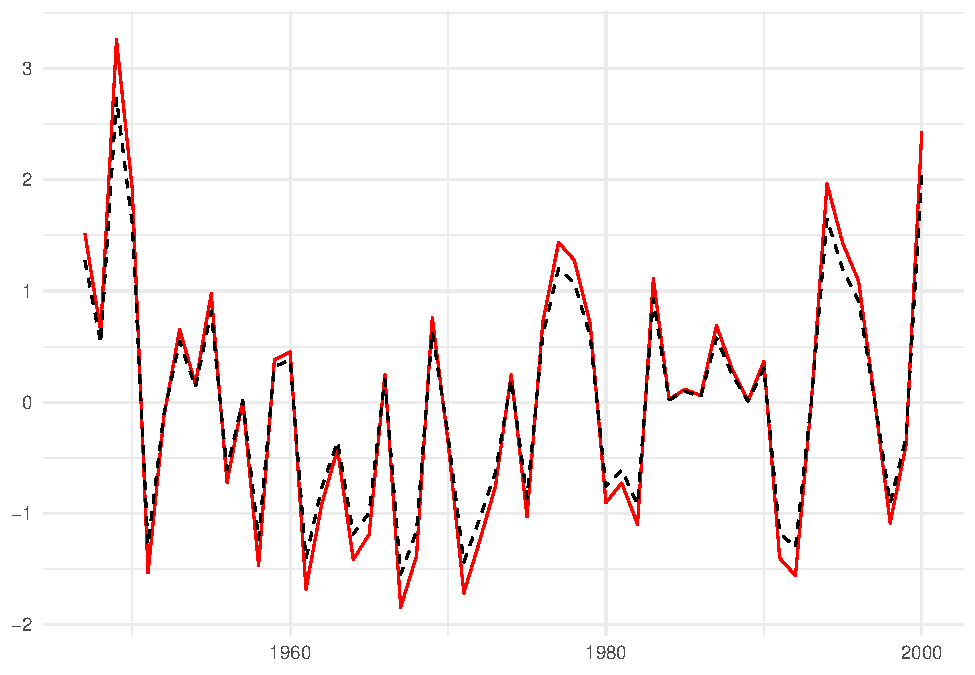
\includegraphics{rEkonometri_files/figure-latex/unnamed-chunk-120-1.pdf}

Yukarıdaki inişli-çıkışlı örüntü, korelasyon sergilemektedir. Ne tür bir korelasyon olduğunu görmek için kalıntıları bir dönem gecikmeleri ile serpilme grafiğine aktaracağız.

\begin{Shaded}
\begin{Highlighting}[]
\NormalTok{df}\OperatorTok{$}\NormalTok{res2 <-}\StringTok{ }\KeywordTok{lag}\NormalTok{(df}\OperatorTok{$}\NormalTok{res)}

\NormalTok{df }\OperatorTok\StringTok{ }
\StringTok{  }\KeywordTok{ggplot}\NormalTok{(}\KeywordTok{aes}\NormalTok{(}\DataTypeTok{x =}\NormalTok{ res2, }\DataTypeTok{y =}\NormalTok{ res)) }\OperatorTok{+}
\StringTok{  }\KeywordTok{geom_point}\NormalTok{(}\DataTypeTok{alpha =} \FloatTok{0.5}\NormalTok{) }\OperatorTok{+}
\StringTok{  }\KeywordTok{geom_smooth}\NormalTok{(}\DataTypeTok{method =} \StringTok{"lm"}\NormalTok{, }\DataTypeTok{se =} \OtherTok{FALSE}\NormalTok{, }\DataTypeTok{color =} \StringTok{"red"}\NormalTok{) }\OperatorTok{+}
\StringTok{  }\KeywordTok{theme_minimal}\NormalTok{()}
\end{Highlighting}
\end{Shaded}

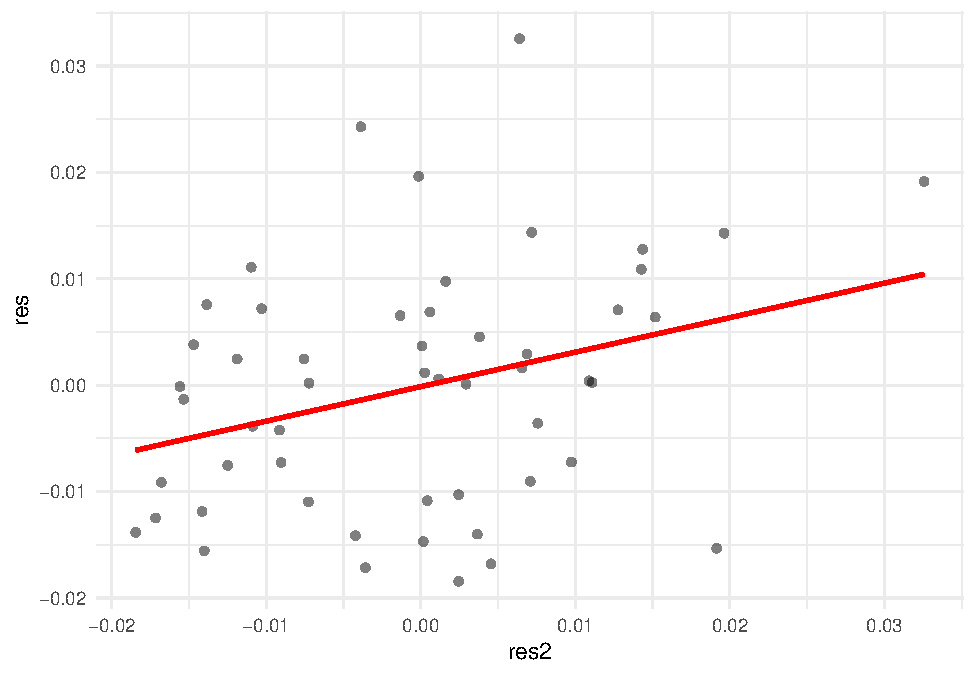
\includegraphics{rEkonometri_files/figure-latex/unnamed-chunk-121-1.pdf}

Kalıntıların pozitif korelasyonlu olduklarını görüyoruz.

Bu yaptığımız ipucu verse de öznel ya da nitel testtir. Bir de nicel testler bulunmaktadır.

\hypertarget{durbin-watson-d}{%
\section{Durbin-Watson d}\label{durbin-watson-d}}

d değeri 0-4 arasındadır. 0'a yakınlık pozitif otokorelasyonun kanıtını artırır; 4'e yakınlık negatif otokorelasyonun kanıtını artırır; 2 civarı pozitif ya da negatif otokorelasyon kanıtı yoktur demektir.

\begin{Shaded}
\begin{Highlighting}[]
\KeywordTok{durbinWatsonTest}\NormalTok{(model)}
\end{Highlighting}
\end{Shaded}

\begin{verbatim}
##  lag Autocorrelation D-W Statistic p-value
##    1       0.2977616      1.289218   0.002
##  Alternative hypothesis: rho != 0
\end{verbatim}

Kurduğumuz model için d istatistiğini 1.29 bulduk. Peki, nasıl karar vereceğiz?

\(d_L\) alt sınır; \(d_U\) ise üst sınır olmak üzere eğer;

\begin{enumerate}
\def\labelenumi{\roman{enumi}.}
\item
  d \textless{} \(d_L\) ise pozitif otokorelasyonun muhtemel kanıtı vardır.
\item
  d \textgreater{} \(d_U\) ise pozitif otokorelasyonun muhtemel kanıtı yoktur.
\item
  \(d_L\) \textless{} d \textless{} \(d_U\) ise pozitif otokorelasyon ile ilgili kesin bir sonuca varılamaz.
\item
  \(d_U\) \textless{} d \textless{} 4 -- \(d_U\) ise pozitif ya da negatif otokorelasyonun muhtemel kanıtı yoktur.
\item
  4 -- \(d_U\) \textless{} d \textless{} 4 -- \(d_L\) ise negatif otokorelasyonla ilgili kesin bir sonuca varılamaz.
\item
  4 -- \(d_L\) \textless{} d \textless{} 4 ise negatif otokorelasyonun muhtemel kanıtı vardır.
\end{enumerate}

Tablo değerlerine \href{https://www3.nd.edu/~wevans1/econ30331/Durbin_Watson_tables.pdf}{buradan} ulaşabilirsiniz. n'i 54 alıyoruz ama tabloda n = 55 alınabilir. k ise bağımsız değişken sayısıdır ki bu da 3'tür. \%5 için d değerleri 1.452 ve 1.681'dir.

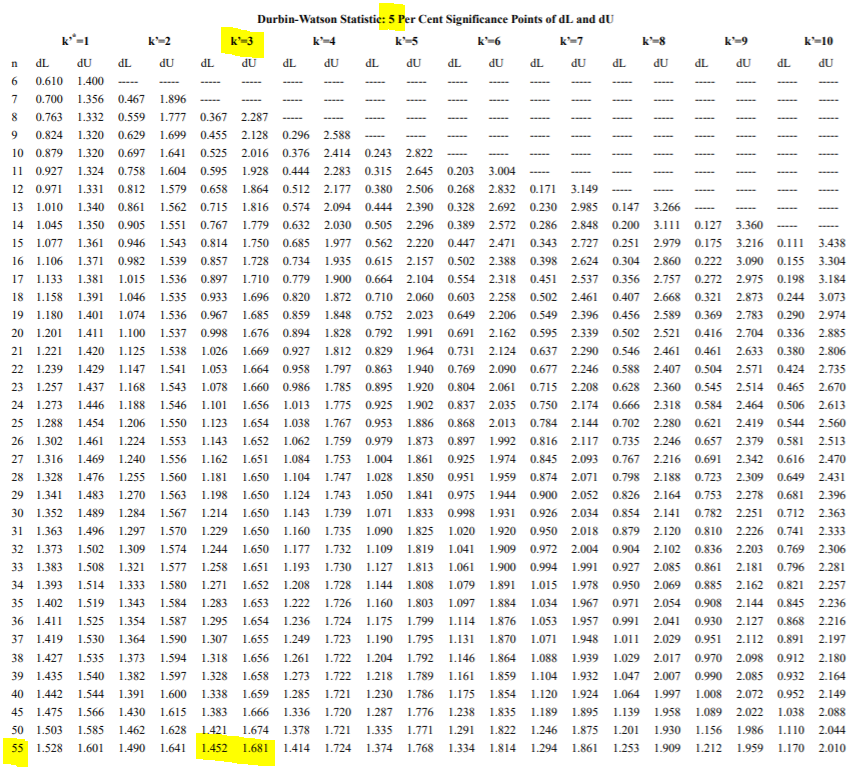
\includegraphics[width=1\linewidth]{C:/Users/datanerd/Desktop/Github/rEkonometri/img/durbin-watson}

Hesapladığımız d değeri 1.29 idi. Bu da alt sınıra yakın demektir. d \textless{} \(d_L\) için pozitif otokorelasyonun muhtemel kanıtı vardır demiştik. Grafik ile de aynı sonuca ulaşmıştık.

Tabi d istatistiğinin varsayımlarını atlamamak gerekiyor:

\begin{enumerate}
\def\labelenumi{\roman{enumi}.}
\item
  Regresyon modeli kesme terimi içerecek.
\item
  Yinelenen örneklemlerde bağımsız değişkenler sabit olacak (hata teriminden bağımsızlık).
\item
  Hata terimi birinci dereceden otoregresif olacak. Yani, bugünkü hata terimi ile bir önceki hata terimi.
\item
  Hata terimi normal dağılımlı olacak.
\item
  Bağımsız değişkenler bağımlı değişkenin gecikmeli değerlerini içermeyecek.
\end{enumerate}

Durbin-Watson d testini kullanamadığımız bir durum vardır. Eğer bu modeli otoregresif model yaparsak; yani, modelde bağımsız değişkenlerden bir tanesi bağımlı değişkenin gecikmeli değerini içeriyorsa bu test kullanılamaz.

\hypertarget{breusch-godfrey}{%
\section{Breusch-Godfrey}\label{breusch-godfrey}}

Bu test ile az önce gördüğümüz testin kısıtlarından kurtulacağız. Bu test ile bağımlı değişkenlerin gecikmeli değerleri bağımsız değişkenlere dahil edilebilecek, daha yüksek mertebeli otoregresifler olabilecek, hata teriminin hareketli ortalama terimlerine imkan tanınabilecek.

Testteki ilk adım Sıradan En Küçük Kareler ile modeli oluşturmak ve kalıntıları bulmaktır. Ardından bu kalıntıların bağımsız değişkenler ile otoregresif terimlere göre regresyonu alınır. Büyük örneklemde \(\chi^2\) dağılımı izler (alternatif olarak F değeri kullanılabilir). \(\chi^2\) değeri belirlenen anlamlılık düzeyindeki kritik değeri aşıyorsa \(H_0\) reddedilir. Bu red de otokorelasyonun varlığına işaret eder. Aynı yorum F için de geçerlidir. p değeri düşükse \(H_0\)'ı reddedebiliriz.

\begin{Shaded}
\begin{Highlighting}[]
\KeywordTok{bgtest}\NormalTok{(model, }\DataTypeTok{order =} \DecValTok{1}\NormalTok{, }\DataTypeTok{type =} \StringTok{"F"}\NormalTok{)}
\end{Highlighting}
\end{Shaded}

\begin{verbatim}
## 
##  Breusch-Godfrey test for serial correlation of order up to 1
## 
## data:  model
## LM test = 5.3462, df1 = 1, df2 = 49, p-value = 0.02501
\end{verbatim}

Sadece bir gecikmeli değer aldık ve F ve \(\chi^2\) için ayrı ayrı gösterdik. p değerleri düşük olması \(H_0\)'ın reddi olup otokorelasyonun varlığına işarettir. Buna ikinci ve üçüncü derecede de bakılabilir.

\begin{Shaded}
\begin{Highlighting}[]
\KeywordTok{bgtest}\NormalTok{(model, }\DataTypeTok{order =} \DecValTok{2}\NormalTok{, }\DataTypeTok{type =} \StringTok{"F"}\NormalTok{)}
\end{Highlighting}
\end{Shaded}

\begin{verbatim}
## 
##  Breusch-Godfrey test for serial correlation of order up to 2
## 
## data:  model
## LM test = 3.2541, df1 = 2, df2 = 48, p-value = 0.04728
\end{verbatim}

\begin{Shaded}
\begin{Highlighting}[]
\KeywordTok{bgtest}\NormalTok{(model, }\DataTypeTok{order =} \DecValTok{2}\NormalTok{, }\DataTypeTok{type =} \StringTok{"Chisq"}\NormalTok{)}
\end{Highlighting}
\end{Shaded}

\begin{verbatim}
## 
##  Breusch-Godfrey test for serial correlation of order up to 2
## 
## data:  model
## LM test = 6.4476, df = 2, p-value = 0.0398
\end{verbatim}

\begin{Shaded}
\begin{Highlighting}[]
\KeywordTok{bgtest}\NormalTok{(model, }\DataTypeTok{order =} \DecValTok{3}\NormalTok{, }\DataTypeTok{type =} \StringTok{"F"}\NormalTok{)}
\end{Highlighting}
\end{Shaded}

\begin{verbatim}
## 
##  Breusch-Godfrey test for serial correlation of order up to 3
## 
## data:  model
## LM test = 2.2032, df1 = 3, df2 = 47, p-value = 0.1001
\end{verbatim}

\begin{Shaded}
\begin{Highlighting}[]
\KeywordTok{bgtest}\NormalTok{(model, }\DataTypeTok{order =} \DecValTok{3}\NormalTok{, }\DataTypeTok{type =} \StringTok{"Chisq"}\NormalTok{)}
\end{Highlighting}
\end{Shaded}

\begin{verbatim}
## 
##  Breusch-Godfrey test for serial correlation of order up to 3
## 
## data:  model
## LM test = 6.6577, df = 3, p-value = 0.08365
\end{verbatim}

İkinci dereceden otoregresifin de istatistiksel olarak anlamlı çıkacağı görülecektir. Bu da ikinci dereceden otoregresif hata yapısının model için daha uygun olduğunu söyler.

Breusch-Godfrey aşağıdaki özelliklere sahiptir:

\begin{enumerate}
\def\labelenumi{\roman{enumi}.}
\item
  Test, bağımsız değişken değerleri ile hata teriminin gecikmeli değerleri verildiğinde hata teriminin sabit varyanslı olduğunu varsayar.
\item
  Testin uygulanmasında pratik bir sorun gecikmeli hata terimlerinin sayısının seçimidir. Bu, zaman serisinin türüne bağlı olabilmektedir. Aylık: 11, çeyrek: 3, yıllık: 1 yeterli olabilir.
\end{enumerate}

Otokorelasyonun varlığını ortaya koyduk. Düzeltmek için neler yapabiliriz?

Birinci fark ya da genelleştirilmiş dönüşüm gibi yöntemler kullanılabilir. Bunlar deneme-yanılma yöntemleridir. Biz düzeltici önlem olarak Newey-West'in Sıradan En Küçük Kareler standart hatalarını düzeltme yöntemini göreceğiz.

\hypertarget{hac-yuxf6ntemi}{%
\section{HAC Yöntemi}\label{hac-yuxf6ntemi}}

Buradaki şart örneklemin büyük olmasıdır. Bu yöntem ile düzeltilen standart hatalar değişen varyans ve otokorelasyon tutarlı standart hatalar (heteroskedasticity and autocorrelation consistent, hac) olarak da bilinir. Genel anlamda, eğer otokorelasyon varsa hac standart hatalarının her zamanki Sıradan En Küçük Kareler standart hatalarından daha büyük olduğu bulunmuştur.

\begin{Shaded}
\begin{Highlighting}[]
\KeywordTok{coeftest}\NormalTok{(model, }\DataTypeTok{vcov =} \KeywordTok{NeweyWest}\NormalTok{(model))}
\end{Highlighting}
\end{Shaded}

\begin{verbatim}
## 
## t test of coefficients:
## 
##                Estimate  Std. Error  t value  Pr(>|t|)    
## (Intercept) -0.46771100  0.04440193 -10.5336 2.716e-14 ***
## lnincome     0.80487293  0.01621446  49.6392 < 2.2e-16 ***
## lnwealth     0.20126996  0.01452512  13.8567 < 2.2e-16 ***
## interest    -0.00268906  0.00082005  -3.2791    0.0019 ** 
## ---
## Signif. codes:  0 '***' 0.001 '**' 0.01 '*' 0.05 '.' 0.1 ' ' 1
\end{verbatim}

Hac yöntemi sadece standart hataları ve dolayısıyla t istatistiklerini ve p değerlerini değiştirir.

Eğer ilk kurduğumuz model ile karşılaştırırsak aralarında önemli bir fark olmadığını göreceğiz. Bu durum değişik otokorelasyon sınamalarına dayanan otokorelasyon kanıtlarına rağmen otokorelasyon sorununun çok ciddi görünmediğini ortaya koyar.

Eğer örneklem genişliği yeterince büyükse, otokorelasyon yapısıyla ilgili herhangi bir özel bilgi gerektirmeyen robust standart hataları ya da hac standart hatalarını kullanabiliriz.

\hypertarget{model-tanux131mlama-hatalarux131}{%
\chapter{Model Tanımlama Hataları}\label{model-tanux131mlama-hatalarux131}}

\begin{quote}
\emph{Uygulamalı ekonometri gözü kapalı yapılamaz; anlama, sezgi, ustalık gerektirir.} -Cuthbertson, Hall, Taylor
\end{quote}

Modelin doğru tanımlanması klasik doğrusal regresyon modeli varsayımlarından biridir.

\begin{Shaded}
\begin{Highlighting}[]
\KeywordTok{library}\NormalTok{(readxl);}\KeywordTok{library}\NormalTok{(tidyverse);}\KeywordTok{library}\NormalTok{(magrittr);}\KeywordTok{library}\NormalTok{(lmtest);}\KeywordTok{library}\NormalTok{(psych);}\KeywordTok{library}\NormalTok{(moments)}

\NormalTok{df <-}\StringTok{ }\KeywordTok{read_excel}\NormalTok{(}\StringTok{"C:/Users/datanerd/Desktop/Github/rEkonometri/data/Table1_1.xls"}\NormalTok{)}
\NormalTok{df }\OperatorTok\StringTok{ }
\StringTok{  }\NormalTok{dplyr}\OperatorTok{::}\KeywordTok{select}\NormalTok{(wage, female, nonwhite, union, education, exper, age)}
\end{Highlighting}
\end{Shaded}

\hypertarget{eksik-tanux131mlanmux131ux15f-modeller}{%
\section{Eksik Tanımlanmış Modeller}\label{eksik-tanux131mlanmux131ux15f-modeller}}

Eksik tanımlı model olursa ne olur?

\begin{itemize}
\item
  Tahmin edilen parametreler yanlıdır ve tutarlı değildir. Bu, dışarıda bırakılan değişkenlerle modeldeki değişkenlerin korelasyonlu olması durumunda geçerlidir.
\item
  Herhangi bir korelasyon olmasa bile modelin kesme terimi yanlıdır.
\item
  Hata varyansı yanlış tahmin edilir.
\item
  Parametre tahminlerine ait varyanslar yanlıdır. Bunun sonucu olarak standart hatalar da yanlıdır.
\item
  Her zamanki güven aralıkları ve hipotez testi yöntemlerinin güvenilirliği azalır ve bu da istatistiksel anlamlılık hakkında yanıltıcı bilgilere yol açar.
\item
  Öngörü ve öngörü güven aralıkları sağlıklı olmaz.
\end{itemize}

Gujarati, \emph{doğru tanımlanmış modeli bulmaya çalışmak kutsal kaseyi bulmaya çalışmak gibidir} der. En iyi yolun ise dikkate alınacak alternatif bir modelle karşılaştırmak olacağını savunur.

\begin{Shaded}
\begin{Highlighting}[]
\NormalTok{df1 <-}\StringTok{ }\NormalTok{df}
\NormalTok{model <-}\StringTok{ }\KeywordTok{lm}\NormalTok{(}\DataTypeTok{formula =}\NormalTok{ wage }\OperatorTok{~}\StringTok{ }\NormalTok{female }\OperatorTok{+}\StringTok{ }\NormalTok{nonwhite }\OperatorTok{+}\StringTok{ }\NormalTok{union }\OperatorTok{+}\StringTok{ }\NormalTok{education }\OperatorTok{+}\StringTok{ }\NormalTok{exper, }\DataTypeTok{data =}\NormalTok{ df1)}
\KeywordTok{summary}\NormalTok{(model)}
\end{Highlighting}
\end{Shaded}

\begin{verbatim}
## 
## Call:
## lm(formula = wage ~ female + nonwhite + union + education + exper, 
##     data = df1)
## 
## Residuals:
##     Min      1Q  Median      3Q     Max 
## -20.781  -3.760  -1.044   2.418  50.414 
## 
## Coefficients:
##             Estimate Std. Error t value Pr(>|t|)    
## (Intercept) -7.18334    1.01579  -7.072 2.51e-12 ***
## female      -3.07488    0.36462  -8.433  < 2e-16 ***
## nonwhite    -1.56531    0.50919  -3.074  0.00216 ** 
## union        1.09598    0.50608   2.166  0.03052 *  
## education    1.37030    0.06590  20.792  < 2e-16 ***
## exper        0.16661    0.01605  10.382  < 2e-16 ***
## ---
## Signif. codes:  0 '***' 0.001 '**' 0.01 '*' 0.05 '.' 0.1 ' ' 1
## 
## Residual standard error: 6.508 on 1283 degrees of freedom
## Multiple R-squared:  0.3233, Adjusted R-squared:  0.3207 
## F-statistic: 122.6 on 5 and 1283 DF,  p-value: < 2.2e-16
\end{verbatim}

wage'in belirleyicileri olarak female, nonwhite, union, education ve exper değişkenlerini kattık.

Şunu biliyoruz: İş deneyimi arttıkça ücretler de artacaktır. Ama şunu bilmiyoruz: İş deneyimi arttıkça ücretler daha yavaş bir oranda mı artar yoksa daha hızlı bir oranda mı? Bunun için iş deneyimini temsil eden exper değişkeninin karesini modele ekleyeceğiz.

\begin{Shaded}
\begin{Highlighting}[]
\NormalTok{df1 }\OperatorTok\StringTok{ }
\StringTok{  }\KeywordTok{mutate}\NormalTok{(}\DataTypeTok{exper2 =}\NormalTok{ exper}\OperatorTok{^}\DecValTok{2}\NormalTok{)}

\NormalTok{model <-}\StringTok{ }\KeywordTok{lm}\NormalTok{(}\DataTypeTok{formula =}\NormalTok{ wage }\OperatorTok{~}\StringTok{ }\NormalTok{female }\OperatorTok{+}\StringTok{ }\NormalTok{nonwhite }\OperatorTok{+}\StringTok{ }\NormalTok{union }\OperatorTok{+}\StringTok{ }\NormalTok{education }\OperatorTok{+}\StringTok{ }\NormalTok{exper }\OperatorTok{+}\StringTok{ }\NormalTok{exper2, }\DataTypeTok{data =}\NormalTok{ df1)}
\KeywordTok{summary}\NormalTok{(model)}
\end{Highlighting}
\end{Shaded}

\begin{verbatim}
## 
## Call:
## lm(formula = wage ~ female + nonwhite + union + education + exper + 
##     exper2, data = df1)
## 
## Residuals:
##     Min      1Q  Median      3Q     Max 
## -19.883  -3.751  -0.855   2.455  50.125 
## 
## Coefficients:
##              Estimate Std. Error t value Pr(>|t|)    
## (Intercept) -8.419035   1.035710  -8.129 1.01e-15 ***
## female      -3.009360   0.361432  -8.326  < 2e-16 ***
## nonwhite    -1.536077   0.504448  -3.045  0.00237 ** 
## union        1.026979   0.501521   2.048  0.04079 *  
## education    1.323745   0.065937  20.076  < 2e-16 ***
## exper        0.424463   0.053580   7.922 5.03e-15 ***
## exper2      -0.006183   0.001227  -5.039 5.34e-07 ***
## ---
## Signif. codes:  0 '***' 0.001 '**' 0.01 '*' 0.05 '.' 0.1 ' ' 1
## 
## Residual standard error: 6.447 on 1282 degrees of freedom
## Multiple R-squared:  0.3365, Adjusted R-squared:  0.3334 
## F-statistic: 108.4 on 6 and 1282 DF,  p-value: < 2.2e-16
\end{verbatim}

Yeni eklediğimiz \(exper^2\) değişkeninin istatistiksel olarak oldukça anlamlı (düşük p değeri) olduğunu görüyoruz. Fakat parametre işaretinin negatif olduğuna dikkat edelim. exper değişkeni pozitif idi. Bu da iş deneyimine bağlı olarak ücretlerin artış gösterdiğini ama azalan oranda bir artış olduğunu göstermektedir.

Aslında \(exper^2\) değişkenini modelden dışlayarak bu değişkenin (belki de değişkenlerin) modelden dışlanması yanlılığına düştük. Şimdi bir de modele cinsiyet ve deneyim arasındaki etkileşimi dahil edelim.

\begin{Shaded}
\begin{Highlighting}[]
\NormalTok{df1 }\OperatorTok\StringTok{ }
\StringTok{  }\KeywordTok{mutate}\NormalTok{(}\DataTypeTok{female_exper =}\NormalTok{ female }\OperatorTok{*}\StringTok{ }\NormalTok{exper)}

\NormalTok{model <-}\StringTok{ }\KeywordTok{lm}\NormalTok{(}\DataTypeTok{formula =}\NormalTok{ wage }\OperatorTok{~}\StringTok{ }\NormalTok{female }\OperatorTok{+}\StringTok{ }\NormalTok{nonwhite }\OperatorTok{+}\StringTok{ }\NormalTok{union }\OperatorTok{+}\StringTok{ }\NormalTok{education }\OperatorTok{+}\StringTok{ }\NormalTok{exper }\OperatorTok{+}\StringTok{ }\NormalTok{exper2 }\OperatorTok{+}\StringTok{ }\NormalTok{female_exper, }\DataTypeTok{data =}\NormalTok{ df1)}
\KeywordTok{summary}\NormalTok{(model)}
\end{Highlighting}
\end{Shaded}

\begin{verbatim}
## 
## Call:
## lm(formula = wage ~ female + nonwhite + union + education + exper + 
##     exper2 + female_exper, data = df1)
## 
## Residuals:
##     Min      1Q  Median      3Q     Max 
## -20.586  -3.644  -0.823   2.365  49.870 
## 
## Coefficients:
##               Estimate Std. Error t value Pr(>|t|)    
## (Intercept)  -9.200668   1.072115  -8.582  < 2e-16 ***
## female       -1.433980   0.680797  -2.106  0.03537 *  
## nonwhite     -1.481891   0.503577  -2.943  0.00331 ** 
## union         0.949027   0.501081   1.894  0.05846 .  
## education     1.318365   0.065801  20.036  < 2e-16 ***
## exper         0.471974   0.056212   8.396  < 2e-16 ***
## exper2       -0.006274   0.001224  -5.125 3.44e-07 ***
## female_exper -0.084151   0.030848  -2.728  0.00646 ** 
## ---
## Signif. codes:  0 '***' 0.001 '**' 0.01 '*' 0.05 '.' 0.1 ' ' 1
## 
## Residual standard error: 6.431 on 1281 degrees of freedom
## Multiple R-squared:  0.3403, Adjusted R-squared:  0.3367 
## F-statistic: 94.41 on 7 and 1281 DF,  p-value: < 2.2e-16
\end{verbatim}

Eklediğimiz female\_exper değişkeninin tıpkı \(exper^2\) değişkeninde olduğu gibi istatistiksel olarak anlamlı olduğunu görüyoruz. Bu yeni değişkenin parametresi negatiftir. Bu da kadınların benzer iş deneyimi olan erkek meslektaşlarına göre daha az kazandığını belirtmektedir.

Peki, orijinal modeli genişletmeye değer mi? Öyle olduğu görülüyor ama bunu F ile de test edebiliriz.

İlk model kısıtlanmış; genişlettiğimiz model ise kısıtlanmamış model olsun.

\(F = \frac{(R^2_{ur} - R^2_r) / m}{(1 - R^2_{ur}) / (n - k)}\)

Burada, \(R^2_{r}\) kısıtlanmış; \(R^2_{ur}\) kısıtlanmamış \(R^2\)'yi temsil etmektedir. Ayrıca m kısıtlama sayısı (kısıtlanmış model 2 değişkeni dışarıda bıraktı), n gözlem sayısı (1289) ve k kısıtlanmamış modeldeki bağımsız değişken sayısıdır (2 tane de sonradan ekledik ve 8 oldu).

\begin{Shaded}
\begin{Highlighting}[]
\KeywordTok{summary}\NormalTok{(}\KeywordTok{lm}\NormalTok{(}\DataTypeTok{formula =}\NormalTok{ wage }\OperatorTok{~}\StringTok{ }\NormalTok{female }\OperatorTok{+}\StringTok{ }\NormalTok{nonwhite }\OperatorTok{+}\StringTok{ }\NormalTok{union }\OperatorTok{+}\StringTok{ }\NormalTok{education }\OperatorTok{+}\StringTok{ }\NormalTok{exper }\OperatorTok{+}\StringTok{ }\NormalTok{exper2 }\OperatorTok{+}\StringTok{ }\NormalTok{female_exper, }\DataTypeTok{data =}\NormalTok{ df1))}\OperatorTok{$}\NormalTok{r.squared }\CommentTok{#Kısıtlanmamış modele ait R2}
\end{Highlighting}
\end{Shaded}

\begin{verbatim}
## [1] 0.3403154
\end{verbatim}

\begin{Shaded}
\begin{Highlighting}[]
\KeywordTok{summary}\NormalTok{(}\KeywordTok{lm}\NormalTok{(}\DataTypeTok{formula =}\NormalTok{ wage }\OperatorTok{~}\StringTok{ }\NormalTok{female }\OperatorTok{+}\StringTok{ }\NormalTok{nonwhite }\OperatorTok{+}\StringTok{ }\NormalTok{union }\OperatorTok{+}\StringTok{ }\NormalTok{education }\OperatorTok{+}\StringTok{ }\NormalTok{exper, }\DataTypeTok{data =}\NormalTok{ df1))}\OperatorTok{$}\NormalTok{r.squared }\CommentTok{#Kısıtlanmış modele ait R2}
\end{Highlighting}
\end{Shaded}

\begin{verbatim}
## [1] 0.3233388
\end{verbatim}

\(F = \frac{((0.3403154 – 0.3233388) / 2)}{((1 – 0.3403154) / (1289 – 8))} = 16.4829\)

F değeri m = 2 pay ve n - k = 1281 payda serbestlik derecesi için oldukça anlamlıdır. Bu da belirlediğimiz iki değişkenin orijinal modele eklenmesini desteklemektedir. Evet, \(R^2\)'lerde önemli bir değişiklik olmadı ama F testi bize bunun önemli olduğunu gösterdi. Biz burada değişkenlerin dışlanması ile orijinal modeldeki parametrelerin yanlı olabileceğini gördük çünkü ilgili değişkenleri ekleyince parametreler de önemli ölçüde değişti. Şunu da bilelim: Örneklem büyüklüğü arttıkça yanlılığın ortadan kalkacağına dair bir garanti yoktur.

Dışlanan değişkenlerle ilgili iki test göreceğiz: Ramsey Reset ve Lagrange Çarpan (LM).

Ramsey Reset:

İlk olarak kurduğumuz modelden tahmin değerlerini elde ederiz. Bu tahmin değerlerinin ikinci, üçüncü ve belki daha yüksek kuvvetlerini bağımsız değişken olarak modele ilave ederek yeniden bir tahminleme yaparız. Ardından F testi ile kısıtlanmış-kısıtlanmamış model yaparız. Eğer F testi istatistiksel olarak anlamlı ise \(H_0\)'ı reddedip kısıtlanmış modelin uygun olmadığını söyleriz.

Önce modeli kuralım. Ardından test edelim.

\begin{Shaded}
\begin{Highlighting}[]
\NormalTok{df1}\OperatorTok{$}\NormalTok{tahmin <-}\StringTok{ }\KeywordTok{lm}\NormalTok{(}\DataTypeTok{formula =}\NormalTok{ wage }\OperatorTok{~}\StringTok{ }\NormalTok{female }\OperatorTok{+}\StringTok{ }\NormalTok{nonwhite }\OperatorTok{+}\StringTok{ }\NormalTok{union }\OperatorTok{+}\StringTok{ }\NormalTok{education }\OperatorTok{+}\StringTok{ }\NormalTok{exper, }\DataTypeTok{data =}\NormalTok{ df1)}\OperatorTok{$}\NormalTok{fitted.values}
\NormalTok{df1}\OperatorTok{$}\NormalTok{tahmin2 <-}\StringTok{ }\NormalTok{df1}\OperatorTok{$}\NormalTok{tahmin}\OperatorTok{^}\DecValTok{2}
\NormalTok{df1}\OperatorTok{$}\NormalTok{tahmin3 <-}\StringTok{ }\NormalTok{df1}\OperatorTok{$}\NormalTok{tahmin}\OperatorTok{^}\DecValTok{3}

\NormalTok{model <-}\StringTok{ }\KeywordTok{lm}\NormalTok{(}\DataTypeTok{formula =}\NormalTok{ wage }\OperatorTok{~}\StringTok{ }\NormalTok{female }\OperatorTok{+}\StringTok{ }\NormalTok{nonwhite }\OperatorTok{+}\StringTok{ }\NormalTok{union }\OperatorTok{+}\StringTok{ }\NormalTok{education }\OperatorTok{+}\StringTok{ }\NormalTok{exper }\OperatorTok{+}\StringTok{ }\NormalTok{tahmin2 }\OperatorTok{+}\StringTok{ }\NormalTok{tahmin3, }\DataTypeTok{data =}\NormalTok{ df1)}
\KeywordTok{summary}\NormalTok{(model)}
\end{Highlighting}
\end{Shaded}

\begin{verbatim}
## 
## Call:
## lm(formula = wage ~ female + nonwhite + union + education + exper + 
##     tahmin2 + tahmin3, data = df1)
## 
## Residuals:
##     Min      1Q  Median      3Q     Max 
## -25.769  -3.483  -0.997   2.324  50.870 
## 
## Coefficients:
##               Estimate Std. Error t value Pr(>|t|)  
## (Intercept)  4.4129809  2.4536171   1.799   0.0723 .
## female      -0.0590166  0.7975349  -0.074   0.9410  
## nonwhite    -0.1954657  0.6316463  -0.309   0.7570  
## union        0.1241080  0.5641605   0.220   0.8259  
## education    0.0801244  0.3023952   0.265   0.7911  
## exper        0.0009687  0.0424703   0.023   0.9818  
## tahmin2      0.0447380  0.0207669   2.154   0.0314 *
## tahmin3     -0.0003106  0.0006007  -0.517   0.6052  
## ---
## Signif. codes:  0 '***' 0.001 '**' 0.01 '*' 0.05 '.' 0.1 ' ' 1
## 
## Residual standard error: 6.413 on 1281 degrees of freedom
## Multiple R-squared:  0.344,  Adjusted R-squared:  0.3404 
## F-statistic: 95.94 on 7 and 1281 DF,  p-value: < 2.2e-16
\end{verbatim}

\begin{Shaded}
\begin{Highlighting}[]
\KeywordTok{resettest}\NormalTok{(}\KeywordTok{lm}\NormalTok{(}\DataTypeTok{formula =}\NormalTok{ wage }\OperatorTok{~}\StringTok{ }\NormalTok{female }\OperatorTok{+}\StringTok{ }\NormalTok{nonwhite }\OperatorTok{+}\StringTok{ }\NormalTok{union }\OperatorTok{+}\StringTok{ }\NormalTok{education }\OperatorTok{+}\StringTok{ }\NormalTok{exper, }\DataTypeTok{data =}\NormalTok{ df1))}
\end{Highlighting}
\end{Shaded}

\begin{verbatim}
## 
##  RESET test
## 
## data:  lm(formula = wage ~ female + nonwhite + union + education + exper,     data = df1)
## RESET = 20.124, df1 = 2, df2 = 1281, p-value = 2.483e-09
\end{verbatim}

F değeri istatistiksel olarak oldukça anlamlıdır (neredeyse sıfır bir p değerine sahip). Bu da \(H_0\)'ın reddi olup model tanımlama hatasına kanıttır.

Ramsey Reset testi bu kanıtı bulsa da alternatif bir yol önermez. Ayrıca modele eklenecek tahmin değerlerinin kuvvetlerinin sayısı hakkında da bilgi vermez.

Şimdi bir de Lagrange Çarpan ya da LM testine bakalım. Bu test için öncelikle orijinal modelden elde edilen kalıntıları buluruz. Eğer model doğruysa kalıntılarla modelden dışlanan değişkenler arasında ilişki olmamalıdır. Ardından kalıntıların orijinal modeldeki ve dışlanan değişkenlere göre regresyonunu alırız. Hesaplanan \(\chi^2\) değeri kritik \(\chi^2\) değerini belirlenen anlamlılık düzeyinde geçerse (p değeri yeterince küçükse) orijinal regresyonu reddederiz. Yani, orijinal model yanlış tanımlanmıştır.

Önce modeli kuralım. Ardından test edelim.

\begin{Shaded}
\begin{Highlighting}[]
\NormalTok{df1}\OperatorTok{$}\StringTok{`}\DataTypeTok{kalıntılar}\StringTok{`}\NormalTok{ <-}\StringTok{ }\KeywordTok{lm}\NormalTok{(}\DataTypeTok{formula =}\NormalTok{ wage }\OperatorTok{~}\StringTok{ }\NormalTok{female }\OperatorTok{+}\StringTok{ }\NormalTok{nonwhite }\OperatorTok{+}\StringTok{ }\NormalTok{union }\OperatorTok{+}\StringTok{ }\NormalTok{education }\OperatorTok{+}\StringTok{ }\NormalTok{exper, }\DataTypeTok{data =}\NormalTok{ df1)}\OperatorTok{$}\NormalTok{residuals}

\NormalTok{model <-}\StringTok{ }\KeywordTok{lm}\NormalTok{(}\DataTypeTok{formula =} \StringTok{`}\DataTypeTok{kalıntılar}\StringTok{`} \OperatorTok{~}\StringTok{ }\NormalTok{female }\OperatorTok{+}\StringTok{ }\NormalTok{nonwhite }\OperatorTok{+}\StringTok{ }\NormalTok{union }\OperatorTok{+}\StringTok{ }\NormalTok{education }\OperatorTok{+}\StringTok{ }\NormalTok{exper }\OperatorTok{+}\StringTok{ }\NormalTok{exper2 }\OperatorTok{+}\StringTok{ }\NormalTok{female_exper, }\DataTypeTok{data =}\NormalTok{ df1)}
\KeywordTok{summary}\NormalTok{(model)}
\end{Highlighting}
\end{Shaded}

\begin{verbatim}
## 
## Call:
## lm(formula = kalıntılar ~ female + nonwhite + union + education + 
##     exper + exper2 + female_exper, data = df1)
## 
## Residuals:
##     Min      1Q  Median      3Q     Max 
## -20.586  -3.644  -0.823   2.365  49.870 
## 
## Coefficients:
##               Estimate Std. Error t value Pr(>|t|)    
## (Intercept)  -2.017330   1.072115  -1.882  0.06011 .  
## female        1.640895   0.680797   2.410  0.01608 *  
## nonwhite      0.083422   0.503577   0.166  0.86845    
## union        -0.146949   0.501081  -0.293  0.76937    
## education    -0.051936   0.065801  -0.789  0.43009    
## exper         0.305367   0.056212   5.432 6.65e-08 ***
## exper2       -0.006274   0.001224  -5.125 3.44e-07 ***
## female_exper -0.084151   0.030848  -2.728  0.00646 ** 
## ---
## Signif. codes:  0 '***' 0.001 '**' 0.01 '*' 0.05 '.' 0.1 ' ' 1
## 
## Residual standard error: 6.431 on 1281 degrees of freedom
## Multiple R-squared:  0.02509,    Adjusted R-squared:  0.01976 
## F-statistic: 4.709 on 7 and 1281 DF,  p-value: 3.126e-05
\end{verbatim}

Gözlem sayısı * \(R^2\) değeri = 1289 * 0.02509 = 32.34101 olup 2 serbestlik derecesi için bu değeri veya daha büyüğünü elde etme olasılığı son derece düşüktür. Bu da Ramsey Reset testini destekleyen bir Lagrange Çarpan testi sonucudur. Yani, orijinal model yanlış belirlenmiştir.

\hypertarget{aux15fux131rux131-tanux131mlanmux131ux15f-modeller}{%
\section{Aşırı Tanımlanmış Modeller}\label{aux15fux131rux131-tanux131mlanmux131ux15f-modeller}}

\(R^2\) yükseldikçe modelin daha iyi olacağına inanılır. Bunun için de modele değişkenler eklenir. Bu da bir modeli aşırı tanımlama sorununa götürebilir.

Aşırı tanımlı model olursa ne olur?

\begin{itemize}
\item
  Aşırı tanımlanmış modelin bütün Sıradan En Küçük Kareler tahmincileri yansızdır ve tutarlıdır.
\item
  Hata terimi varyansı doğru tahmin edilir.
\item
  Güven aralığı ve hipotez testleri güvenilirdir.
\item
  Ancak böyle bir modelin parametre tahminleri genelde etkin değildir. Yani, varyanslar gerçek modelinkilerden daha yüksektir.
\end{itemize}

Aşırı tanımlı modelde şunu bilmek gerekiyor: Hem tahmincilerde etkinlik kaybı söz konusu olacak hem de çoklu doğrusal bağlantı sorununu doğurabilir.

Bunu anlatabilmek için aynı örnek üzerinden gidelim. Veri setini tekrar alalım ve bu defa age değişkenini de ekleyelim.

\begin{Shaded}
\begin{Highlighting}[]
\NormalTok{df2 <-}\StringTok{ }\NormalTok{df}

\NormalTok{model <-}\StringTok{ }\KeywordTok{lm}\NormalTok{(}\DataTypeTok{formula =}\NormalTok{ wage }\OperatorTok{~}\StringTok{ }\NormalTok{female }\OperatorTok{+}\StringTok{ }\NormalTok{nonwhite }\OperatorTok{+}\StringTok{ }\NormalTok{union }\OperatorTok{+}\StringTok{ }\NormalTok{education }\OperatorTok{+}\StringTok{ }\NormalTok{exper }\OperatorTok{+}\StringTok{ }\NormalTok{age, }\DataTypeTok{data =}\NormalTok{ df2)}
\KeywordTok{summary}\NormalTok{(model)}
\end{Highlighting}
\end{Shaded}

\begin{verbatim}
## 
## Call:
## lm(formula = wage ~ female + nonwhite + union + education + exper + 
##     age, data = df2)
## 
## Residuals:
##     Min      1Q  Median      3Q     Max 
## -20.781  -3.760  -1.044   2.418  50.414 
## 
## Coefficients: (1 not defined because of singularities)
##             Estimate Std. Error t value Pr(>|t|)    
## (Intercept) -7.18334    1.01579  -7.072 2.51e-12 ***
## female      -3.07488    0.36462  -8.433  < 2e-16 ***
## nonwhite    -1.56531    0.50919  -3.074  0.00216 ** 
## union        1.09598    0.50608   2.166  0.03052 *  
## education    1.37030    0.06590  20.792  < 2e-16 ***
## exper        0.16661    0.01605  10.382  < 2e-16 ***
## age               NA         NA      NA       NA    
## ---
## Signif. codes:  0 '***' 0.001 '**' 0.01 '*' 0.05 '.' 0.1 ' ' 1
## 
## Residual standard error: 6.508 on 1283 degrees of freedom
## Multiple R-squared:  0.3233, Adjusted R-squared:  0.3207 
## F-statistic: 122.6 on 5 and 1283 DF,  p-value: < 2.2e-16
\end{verbatim}

age ve exper arasındaki tama yakın doğrusal bağlantı nedeniyle regresyonu çalıştıramadık. Hatırlayın, exper değişkeni = yaş -- eğitim süresi -- 6 okula başlama yaşı olarak tanımlanmıştı. age ve exper değişkenleri arasındaki korelasyon:

\begin{Shaded}
\begin{Highlighting}[]
\KeywordTok{cor}\NormalTok{(df2}\OperatorTok{$}\NormalTok{exper, df2}\OperatorTok{$}\NormalTok{age)}
\end{Highlighting}
\end{Shaded}

\begin{verbatim}
## [1] 0.970575
\end{verbatim}

age veya exper değişkenini modele ekleyebilir ama her ikisini birden tama yakın doğrusal bağlantı nedeniyle modele ekleyemeyiz.

\hypertarget{yanlux131ux15f-fonksiyon-yapux131sux131}{%
\section{Yanlış Fonksiyon Yapısı}\label{yanlux131ux15f-fonksiyon-yapux131sux131}}

Saatlik ücretler ile ilgili iki tane regresyon modeli kurmuştuk: Doğrusal ve Log-Doğrusal.

\begin{Shaded}
\begin{Highlighting}[]
\NormalTok{df3 <-}\StringTok{ }\NormalTok{df }\OperatorTok\StringTok{ }
\StringTok{  }\NormalTok{dplyr}\OperatorTok{::}\KeywordTok{select}\NormalTok{(wage, female, nonwhite, union, education, exper) }\OperatorTok\StringTok{ }
\StringTok{  }\KeywordTok{mutate}\NormalTok{(}\DataTypeTok{exper2 =}\NormalTok{ exper}\OperatorTok{^}\DecValTok{2}\NormalTok{,}
         \DataTypeTok{female_exper =}\NormalTok{ female }\OperatorTok{*}\StringTok{ }\NormalTok{exper,}
         \DataTypeTok{lnwage =} \KeywordTok{log}\NormalTok{(wage))}
\end{Highlighting}
\end{Shaded}

Doğrusal model:

\begin{Shaded}
\begin{Highlighting}[]
\NormalTok{linmodel <-}\StringTok{ }\KeywordTok{lm}\NormalTok{(}\DataTypeTok{formula =}\NormalTok{ wage }\OperatorTok{~}\NormalTok{., }\DataTypeTok{data =}\NormalTok{ df3[,}\OperatorTok{-}\DecValTok{9}\NormalTok{]) }\CommentTok{#9. sütunu alma.}
\KeywordTok{summary}\NormalTok{(linmodel)}
\end{Highlighting}
\end{Shaded}

\begin{verbatim}
## 
## Call:
## lm(formula = wage ~ ., data = df3[, -9])
## 
## Residuals:
##     Min      1Q  Median      3Q     Max 
## -20.586  -3.644  -0.823   2.365  49.870 
## 
## Coefficients:
##               Estimate Std. Error t value Pr(>|t|)    
## (Intercept)  -9.200668   1.072115  -8.582  < 2e-16 ***
## female       -1.433980   0.680797  -2.106  0.03537 *  
## nonwhite     -1.481891   0.503577  -2.943  0.00331 ** 
## union         0.949027   0.501081   1.894  0.05846 .  
## education     1.318365   0.065801  20.036  < 2e-16 ***
## exper         0.471974   0.056212   8.396  < 2e-16 ***
## exper2       -0.006274   0.001224  -5.125 3.44e-07 ***
## female_exper -0.084151   0.030848  -2.728  0.00646 ** 
## ---
## Signif. codes:  0 '***' 0.001 '**' 0.01 '*' 0.05 '.' 0.1 ' ' 1
## 
## Residual standard error: 6.431 on 1281 degrees of freedom
## Multiple R-squared:  0.3403, Adjusted R-squared:  0.3367 
## F-statistic: 94.41 on 7 and 1281 DF,  p-value: < 2.2e-16
\end{verbatim}

Log-Doğrusal model:

\begin{Shaded}
\begin{Highlighting}[]
\NormalTok{loglinmodel <-}\StringTok{ }\KeywordTok{lm}\NormalTok{(}\DataTypeTok{formula =}\NormalTok{ lnwage }\OperatorTok{~}\NormalTok{., }\DataTypeTok{data =}\NormalTok{ df3[,}\OperatorTok{-}\DecValTok{1}\NormalTok{]) }\CommentTok{#1. sütunu alma.}
\KeywordTok{summary}\NormalTok{(loglinmodel)}
\end{Highlighting}
\end{Shaded}

\begin{verbatim}
## 
## Call:
## lm(formula = lnwage ~ ., data = df3[, -1])
## 
## Residuals:
##      Min       1Q   Median       3Q      Max 
## -2.35597 -0.26963  0.01568  0.29182  1.87681 
## 
## Coefficients:
##                Estimate Std. Error t value Pr(>|t|)    
## (Intercept)   7.324e-01  7.761e-02   9.437  < 2e-16 ***
## female       -1.481e-01  4.928e-02  -3.004 0.002715 ** 
## nonwhite     -1.273e-01  3.646e-02  -3.492 0.000496 ***
## union         1.685e-01  3.627e-02   4.645 3.76e-06 ***
## education     9.479e-02  4.764e-03  19.900  < 2e-16 ***
## exper         4.195e-02  4.069e-03  10.308  < 2e-16 ***
## exper2       -6.370e-04  8.863e-05  -7.187 1.12e-12 ***
## female_exper -5.043e-03  2.233e-03  -2.258 0.024109 *  
## ---
## Signif. codes:  0 '***' 0.001 '**' 0.01 '*' 0.05 '.' 0.1 ' ' 1
## 
## Residual standard error: 0.4656 on 1281 degrees of freedom
## Multiple R-squared:  0.373,  Adjusted R-squared:  0.3696 
## F-statistic: 108.9 on 7 and 1281 DF,  p-value: < 2.2e-16
\end{verbatim}

İki model de çok cazip duruyor. Biz bunlardan hangisini seçmeliyiz?

\(R^2\)'lerini karşılaştırabilir miyiz?

Hayır cevabını daha önce vermiştik. \(R^2\) doğrusal modelde bağımlı değişkendeki değişkenliğin bütün bağımsız değişkenlerce açıklanan oranını ölçerken, yarı-logaritmik modelde bağımlı değişkenin logaritmasındaki değişkenliğin oranını ölçer. Bu ikisi aynı şey değildir.

Şu adımları izleyelim.

\begin{enumerate}
\def\labelenumi{\roman{enumi}.}
\tightlist
\item
  Bağımlı değişken wage'lerin geometrik ortalamasını alalım.
\end{enumerate}

\begin{Shaded}
\begin{Highlighting}[]
\KeywordTok{geometric.mean}\NormalTok{(df3}\OperatorTok{$}\NormalTok{wage)}
\end{Highlighting}
\end{Shaded}

\begin{verbatim}
## [1] 10.40634
\end{verbatim}

\begin{Shaded}
\begin{Highlighting}[]
\CommentTok{#ya da}
\KeywordTok{exp}\NormalTok{(}\KeywordTok{mean}\NormalTok{(}\KeywordTok{log}\NormalTok{(df3}\OperatorTok{$}\NormalTok{wage)))}
\end{Highlighting}
\end{Shaded}

\begin{verbatim}
## [1] 10.40634
\end{verbatim}

\begin{enumerate}
\def\labelenumi{\roman{enumi}.}
\setcounter{enumi}{1}
\tightlist
\item
  wage'leri bu geometrik ortalamaya bölelim.
\end{enumerate}

\begin{Shaded}
\begin{Highlighting}[]
\NormalTok{df3}\OperatorTok{$}\NormalTok{go_wage <-}\StringTok{ }\NormalTok{df3}\OperatorTok{$}\NormalTok{wage }\OperatorTok{/}\StringTok{ }\KeywordTok{exp}\NormalTok{(}\KeywordTok{mean}\NormalTok{(}\KeywordTok{log}\NormalTok{(df3}\OperatorTok{$}\NormalTok{wage)))}
\end{Highlighting}
\end{Shaded}

\begin{enumerate}
\def\labelenumi{\roman{enumi}.}
\setcounter{enumi}{2}
\tightlist
\item
  Artık bağımlı değişken wage yerine geometrik ortalamaya bölünmüş wage'i kullanarak modeli yeniden oluşturalım.
\end{enumerate}

\begin{Shaded}
\begin{Highlighting}[]
\NormalTok{yenimodel <-}\StringTok{ }\KeywordTok{lm}\NormalTok{(}\DataTypeTok{formula =}\NormalTok{ go_wage }\OperatorTok{~}\NormalTok{., }\DataTypeTok{data =}\NormalTok{ df3[,}\OperatorTok{-}\KeywordTok{c}\NormalTok{(}\DecValTok{1}\NormalTok{,}\DecValTok{9}\NormalTok{)]) }\CommentTok{#1. ve 9. sütunları alma}
\end{Highlighting}
\end{Shaded}

Buradan kalıntı kareler toplamını elde edelim. Yani, kalıntıların karelerini alıp toplayacağız.

\begin{Shaded}
\begin{Highlighting}[]
\KeywordTok{sum}\NormalTok{((yenimodel}\OperatorTok{$}\NormalTok{residuals)}\OperatorTok{^}\DecValTok{2}\NormalTok{)}
\end{Highlighting}
\end{Shaded}

\begin{verbatim}
## [1] 489.2251
\end{verbatim}

\begin{enumerate}
\def\labelenumi{\roman{enumi}.}
\setcounter{enumi}{3}
\tightlist
\item
  Bağımlı değişken lnwage yerine geometrik ortalamaya bölünmüş wage'in logaritmasını kullanıp model kuralım ve yine yukarıda olduğu gibi kalıntı kareler toplamını elde edelim.
\end{enumerate}

\begin{Shaded}
\begin{Highlighting}[]
\NormalTok{df3}\OperatorTok{$}\NormalTok{go_lnwage <-}\StringTok{ }\KeywordTok{log}\NormalTok{(df3}\OperatorTok{$}\NormalTok{go_wage)}
\NormalTok{yenimodel2 <-}\StringTok{ }\KeywordTok{lm}\NormalTok{(}\DataTypeTok{formula =}\NormalTok{ go_lnwage }\OperatorTok{~}\NormalTok{., }\DataTypeTok{data =}\NormalTok{ df3[,}\OperatorTok{-}\KeywordTok{c}\NormalTok{(}\DecValTok{1}\NormalTok{,}\DecValTok{9}\NormalTok{,}\DecValTok{10}\NormalTok{)]) }\CommentTok{#1., 9. ve 10. sütunları alma}

\KeywordTok{sum}\NormalTok{((yenimodel2}\OperatorTok{$}\NormalTok{residuals)}\OperatorTok{^}\DecValTok{2}\NormalTok{)}
\end{Highlighting}
\end{Shaded}

\begin{verbatim}
## [1] 277.6474
\end{verbatim}

\begin{enumerate}
\def\labelenumi{\alph{enumi}.}
\setcounter{enumi}{21}
\tightlist
\item
  Kalıntı kareler toplamı olan RSS'ler bulunduktan sonra aşağıdaki değeri hesaplayalım.
\end{enumerate}

\(λ = \frac{n}{2} * ln(\frac{RSS_1}{RSS_2})\sim\chi^2_1\)

n gözlem sayısıdır.

Büyük olan RSS değeri paya koyulur.

\begin{Shaded}
\begin{Highlighting}[]
\KeywordTok{nrow}\NormalTok{(df3) }\OperatorTok{/}\StringTok{ }\DecValTok{2} \OperatorTok{*}\StringTok{ }\KeywordTok{log}\NormalTok{(}\KeywordTok{sum}\NormalTok{(yenimodel}\OperatorTok{$}\NormalTok{residuals}\OperatorTok{^}\DecValTok{2}\NormalTok{) }\OperatorTok{/}\StringTok{ }\KeywordTok{sum}\NormalTok{(yenimodel2}\OperatorTok{$}\NormalTok{residuals}\OperatorTok{^}\DecValTok{2}\NormalTok{))}
\end{Highlighting}
\end{Shaded}

\begin{verbatim}
## [1] 365.0904
\end{verbatim}

1 serbestlik derecesi için bu \(\chi^2\) değeri oldukça yüksektir. Bu da istatistiksel olarak anlamlı olup küçük RSS'e sahip modelin daha iyi olduğu sonucunu destekler. Yani, ilk başta kurduğumuz modelin fonksiyon kalıbı yanlış seçilmiştir. Artık log-doğrusal modeli kullanacağız. Log-Doğrusal modelin daha üstün olduğunu istatistiksel olarak göstermiş olduk.

\hypertarget{uxf6luxe7uxfcm-hatalarux131}{%
\section{Ölçüm Hataları}\label{uxf6luxe7uxfcm-hatalarux131}}

Verileri derlerken çok dikkatli ve bazı aşikar hataların giderildiğinden emin olunmalıdır. Eğer bu hatalar bağımlı değişkenlere aitse Sıradan En Küçük Kareler tahmini üzerinde çok ciddi etkileri olmaz. Yani, Sıradan En Küçük Kareler tahmincileri, varyansları ve standart hataları yansızdır ama tahmin edilen varyanslar ve dolayısıyla standart hatalar ölçüm hatalarının olmamasına göre daha büyüktür. Eğer ölçüm hataları bağımsız değişkenlere aitse Sıradan En Küçük Kareler tahmincileri hem yanlı olma hem tutarlı olmama gibi durumlara girer. Hatta tek bir bağımsız değişken diğer bağımsız değişkenlerin yanlı olmasına ve tutarlı olmamasına yol açar.

\begin{quote}
\emph{Hükümetler istatistik biriktirmeye son derece meraklıdır. Onları toplarlar, eklerler, n.~kuvvete yükseltirler, küp kökünü alırlar ve harika diagramlar oluştururlar. Ancak hiçbir zaman unutmamamız gereken bir gerçek bu rakamların her birinin başlangıçta ne bildirdiğini pek de umursamayan köy bekçisi (village watchman) tarafından oluşturulduğudur.} -Stamp
\end{quote}

\hypertarget{aykux131rux131-deux11fer-yuxfcksek-kaldux131rauxe7-etkisi-baskux131n-nokta-ve-simuxfcle-edilmiux15f-veriler}{%
\section{Aykırı Değer, Yüksek Kaldıraç Etkisi, Baskın Nokta ve Simüle Edilmiş Veriler}\label{aykux131rux131-deux11fer-yuxfcksek-kaldux131rauxe7-etkisi-baskux131n-nokta-ve-simuxfcle-edilmiux15f-veriler}}

Regresyon analizi bazında kalıntısı diğer gözlemlerin kalıntılarından büyük olan gözleme aykırı değer denir. Tabi birden fazla olabilir. İşaretleri ortadan kaldırmak için kalıntılara kareleri alınarak da bakılabilir.

Eğer bir gözlem örneklemdeki gözlem yığınlarından aşırı derecede uzaktaysa yüksek kaldıraç etkisi ortaya koyabilir. Bu tür gözlemler regresyon doğrusunu kendine doğru çekebilir ve doğrunun eğiminde değişimlere yol açabilir.

Eğer gözlem, kaldıraç etkisiyle regresyon doğrusunu kendine çekerse buna baskın nokta adı verilir.

\begin{Shaded}
\begin{Highlighting}[]
\NormalTok{ulke <-}\StringTok{ }\KeywordTok{c}\NormalTok{(}\StringTok{"ABD"}\NormalTok{, }\StringTok{"Avustralya"}\NormalTok{, }\StringTok{"Büyük Britanya"}\NormalTok{, }\StringTok{"Danimarka"}\NormalTok{, }\StringTok{"Finlandiya"}\NormalTok{, }\StringTok{"Hollanda"}\NormalTok{, }\StringTok{"İsveç"}\NormalTok{, }\StringTok{"İsviçre"}\NormalTok{, }\StringTok{"İzlanda"}\NormalTok{, }\StringTok{"Kanada"}\NormalTok{, }\StringTok{"Norveç"}\NormalTok{)}
\NormalTok{kisibasinasigara <-}\StringTok{ }\KeywordTok{c}\NormalTok{(}\DecValTok{1300}\NormalTok{, }\DecValTok{480}\NormalTok{, }\DecValTok{1100}\NormalTok{, }\DecValTok{380}\NormalTok{, }\DecValTok{1100}\NormalTok{, }\DecValTok{490}\NormalTok{, }\DecValTok{300}\NormalTok{, }\DecValTok{510}\NormalTok{, }\DecValTok{230}\NormalTok{, }\DecValTok{500}\NormalTok{, }\DecValTok{250}\NormalTok{)}
\NormalTok{milyondaolumoranlari <-}\StringTok{ }\KeywordTok{c}\NormalTok{(}\DecValTok{200}\NormalTok{, }\DecValTok{180}\NormalTok{, }\DecValTok{460}\NormalTok{, }\DecValTok{170}\NormalTok{, }\DecValTok{350}\NormalTok{, }\DecValTok{240}\NormalTok{, }\DecValTok{110}\NormalTok{, }\DecValTok{250}\NormalTok{, }\DecValTok{60}\NormalTok{, }\DecValTok{150}\NormalTok{, }\DecValTok{90}\NormalTok{)}
\NormalTok{df4 <-}\StringTok{ }\KeywordTok{data.frame}\NormalTok{(}\DataTypeTok{ulke =}\NormalTok{ ulke, }\DataTypeTok{kisibasinasigara =}\NormalTok{ kisibasinasigara, }\DataTypeTok{milyondaolumoranlari =}\NormalTok{ milyondaolumoranlari)}

\NormalTok{df4 }\OperatorTok\StringTok{ }
\StringTok{  }\KeywordTok{ggplot}\NormalTok{(}\KeywordTok{aes}\NormalTok{(}\DataTypeTok{x =}\NormalTok{ kisibasinasigara, }\DataTypeTok{y =}\NormalTok{ milyondaolumoranlari)) }\OperatorTok{+}
\StringTok{  }\KeywordTok{geom_point}\NormalTok{(}\DataTypeTok{size =} \DecValTok{3}\NormalTok{) }\OperatorTok{+}
\StringTok{  }\NormalTok{ggrepel}\OperatorTok{::}\KeywordTok{geom_label_repel}\NormalTok{(}\KeywordTok{aes}\NormalTok{(}\DataTypeTok{label =}\NormalTok{ ulke)) }\OperatorTok{+}
\StringTok{  }\KeywordTok{geom_smooth}\NormalTok{(}\DataTypeTok{method =} \StringTok{"lm"}\NormalTok{, }\DataTypeTok{se =} \OtherTok{FALSE}\NormalTok{, }\DataTypeTok{color =} \StringTok{"red"}\NormalTok{) }\OperatorTok{+}
\StringTok{  }\KeywordTok{theme_minimal}\NormalTok{() }\OperatorTok{+}
\StringTok{  }\KeywordTok{labs}\NormalTok{(}\DataTypeTok{x =} \StringTok{"Kişi Başına Sigara"}\NormalTok{, }\DataTypeTok{y =} \StringTok{"1 Milyonda Ölüm Oranı"}\NormalTok{)}
\end{Highlighting}
\end{Shaded}

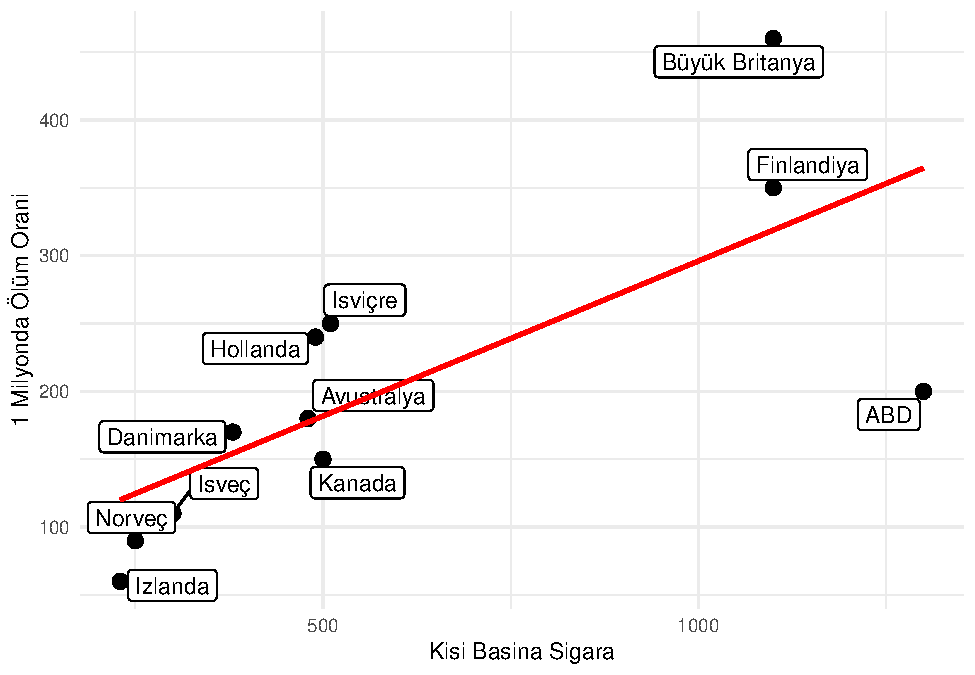
\includegraphics{rEkonometri_files/figure-latex/unnamed-chunk-146-1.pdf}

ABD, sigara tüketiminin en yüksek olduğu yer fakat ölüm oranı nispeten düşük. Aykırı değer diyebilir miyiz? ABD'nin olduğu ve olmadığı iki farklı model kuralım.

\begin{Shaded}
\begin{Highlighting}[]
\NormalTok{abdli_model <-}\StringTok{ }\KeywordTok{lm}\NormalTok{(}\DataTypeTok{formula =}\NormalTok{ milyondaolumoranlari }\OperatorTok{~}\StringTok{ }\NormalTok{kisibasinasigara, }\DataTypeTok{data =}\NormalTok{ df4)}
\KeywordTok{summary}\NormalTok{(abdli_model)}
\end{Highlighting}
\end{Shaded}

\begin{verbatim}
## 
## Call:
## lm(formula = milyondaolumoranlari ~ kisibasinasigara, data = df4)
## 
## Residuals:
##      Min       1Q   Median       3Q      Max 
## -164.531  -33.225    2.789   45.831  141.157 
## 
## Coefficients:
##                  Estimate Std. Error t value Pr(>|t|)   
## (Intercept)      67.56087   49.06048   1.377  0.20176   
## kisibasinasigara  0.22844    0.06976   3.275  0.00961 **
## ---
## Signif. codes:  0 '***' 0.001 '**' 0.01 '*' 0.05 '.' 0.1 ' ' 1
## 
## Residual standard error: 83.49 on 9 degrees of freedom
## Multiple R-squared:  0.5437, Adjusted R-squared:  0.493 
## F-statistic: 10.72 on 1 and 9 DF,  p-value: 0.009612
\end{verbatim}

Bu çıktı sigara ile ölüm oranları arasında pozitif bir ilişki (nedensellik değil) ortaya koyuyor. İstatistiksel olarak da anlamlı olduğunu görüyoruz.

\begin{Shaded}
\begin{Highlighting}[]
\NormalTok{abdsiz_model <-}\StringTok{ }\KeywordTok{lm}\NormalTok{(}\DataTypeTok{formula =}\NormalTok{ milyondaolumoranlari }\OperatorTok{~}\StringTok{ }\NormalTok{kisibasinasigara, }\DataTypeTok{data =}\NormalTok{ df4[}\OperatorTok{-}\DecValTok{1}\NormalTok{,])}
\KeywordTok{summary}\NormalTok{(abdsiz_model)}
\end{Highlighting}
\end{Shaded}

\begin{verbatim}
## 
## Call:
## lm(formula = milyondaolumoranlari ~ kisibasinasigara, data = df4[-1, 
##     ])
## 
## Residuals:
##     Min      1Q  Median      3Q     Max 
## -64.658 -28.273  -7.914  39.200  52.848 
## 
## Coefficients:
##                  Estimate Std. Error t value Pr(>|t|)    
## (Intercept)        9.1393    28.2331   0.324    0.754    
## kisibasinasigara   0.3686     0.0461   7.996 4.38e-05 ***
## ---
## Signif. codes:  0 '***' 0.001 '**' 0.01 '*' 0.05 '.' 0.1 ' ' 1
## 
## Residual standard error: 43.71 on 8 degrees of freedom
## Multiple R-squared:  0.8888, Adjusted R-squared:  0.8749 
## F-statistic: 63.94 on 1 and 8 DF,  p-value: 4.381e-05
\end{verbatim}

Modeli ABD olmadan kurduğumuz zaman parametre değerlerinin, standart hataların ve \(R^2\) değerinin oldukça farklılaştığını görüyoruz. Aslında ABD aynı zamanda baskın noktadır. Aşağıdaki görsel ise ABD olmadan çizilmiştir.

\begin{Shaded}
\begin{Highlighting}[]
\NormalTok{df4 }\OperatorTok\StringTok{ }
\StringTok{  }\KeywordTok{filter}\NormalTok{(ulke }\OperatorTok{!=}\StringTok{ "ABD"}\NormalTok{) }\OperatorTok\StringTok{ }
\StringTok{  }\KeywordTok{ggplot}\NormalTok{(}\KeywordTok{aes}\NormalTok{(}\DataTypeTok{x =}\NormalTok{ kisibasinasigara, }\DataTypeTok{y =}\NormalTok{ milyondaolumoranlari)) }\OperatorTok{+}
\StringTok{  }\KeywordTok{geom_point}\NormalTok{(}\DataTypeTok{size =} \DecValTok{3}\NormalTok{) }\OperatorTok{+}
\StringTok{  }\NormalTok{ggrepel}\OperatorTok{::}\KeywordTok{geom_label_repel}\NormalTok{(}\KeywordTok{aes}\NormalTok{(}\DataTypeTok{label =}\NormalTok{ ulke)) }\OperatorTok{+}
\StringTok{  }\KeywordTok{geom_smooth}\NormalTok{(}\DataTypeTok{method =} \StringTok{"lm"}\NormalTok{, }\DataTypeTok{se =} \OtherTok{FALSE}\NormalTok{, }\DataTypeTok{color =} \StringTok{"red"}\NormalTok{) }\OperatorTok{+}
\StringTok{  }\KeywordTok{theme_minimal}\NormalTok{() }\OperatorTok{+}
\StringTok{  }\KeywordTok{labs}\NormalTok{(}\DataTypeTok{x =} \StringTok{"Kişi Başına Sigara"}\NormalTok{, }\DataTypeTok{y =} \StringTok{"1 Milyonda Ölüm Oranı"}\NormalTok{)}
\end{Highlighting}
\end{Shaded}

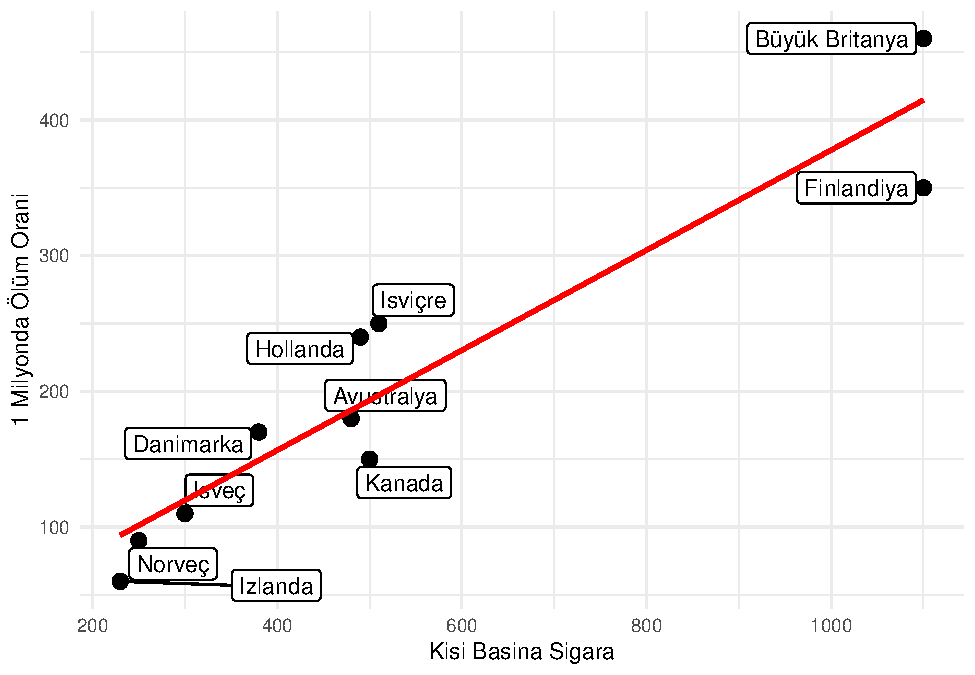
\includegraphics{rEkonometri_files/figure-latex/unnamed-chunk-149-1.pdf}

Buradan aykırı değerlerin gereksiz olduğu ve atılması gerektiği sonucu çıkmasın. Her zaman değil!

Aşağıda simüle edilmiş verilerle çalışacağız. Üç tanımı da anladık ama bunları birbirleri ile karıştırmamak gerekiyor.

0 ile 5 arasında 20 tane veri elde edelim. Bunlar bağımsız değişkene ait olsun. Ardından da 1 + 3x + \(\epsilon_i\) ile de \(Y_i\) değerlerini belirleyelim. Gerçek parametrelerimiz \(β_0\) = 1 ve \(β_1\) = 3.

\begin{Shaded}
\begin{Highlighting}[]
\KeywordTok{set.seed}\NormalTok{(}\DecValTok{1}\NormalTok{)}
\NormalTok{n <-}\StringTok{ }\DecValTok{20}
\NormalTok{x <-}\StringTok{ }\KeywordTok{runif}\NormalTok{(n, }\DataTypeTok{min=}\DecValTok{0}\NormalTok{, }\DataTypeTok{max=}\DecValTok{5}\NormalTok{)}
\NormalTok{y <-}\StringTok{ }\DecValTok{1} \OperatorTok{+}\StringTok{ }\DecValTok{3}\OperatorTok{*}\NormalTok{x }\OperatorTok{+}\StringTok{ }\KeywordTok{rnorm}\NormalTok{(n,}\DecValTok{0}\NormalTok{,}\DecValTok{1}\NormalTok{)}
\NormalTok{df5 <-}\StringTok{ }\KeywordTok{data.frame}\NormalTok{(}\DataTypeTok{y=}\NormalTok{y, }\DataTypeTok{x=}\NormalTok{x)}
\end{Highlighting}
\end{Shaded}

Doğrusal regresyon modelini kuralım.

\begin{Shaded}
\begin{Highlighting}[]
\NormalTok{model1 <-}\StringTok{ }\KeywordTok{lm}\NormalTok{(}\DataTypeTok{formula =}\NormalTok{ y }\OperatorTok{~}\StringTok{ }\NormalTok{x, }\DataTypeTok{data =}\NormalTok{ df5)}
\KeywordTok{summary}\NormalTok{(model1)}
\end{Highlighting}
\end{Shaded}

\begin{verbatim}
## 
## Call:
## lm(formula = y ~ x, data = df5)
## 
## Residuals:
##     Min      1Q  Median      3Q     Max 
## -2.3192 -0.3494  0.1744  0.5882  1.0544 
## 
## Coefficients:
##             Estimate Std. Error t value Pr(>|t|)    
## (Intercept)   1.9412     0.4593   4.226 0.000508 ***
## x             2.6817     0.1479  18.135 5.18e-13 ***
## ---
## Signif. codes:  0 '***' 0.001 '**' 0.01 '*' 0.05 '.' 0.1 ' ' 1
## 
## Residual standard error: 0.9221 on 18 degrees of freedom
## Multiple R-squared:  0.9481, Adjusted R-squared:  0.9452 
## F-statistic: 328.9 on 1 and 18 DF,  p-value: 5.181e-13
\end{verbatim}

\begin{Shaded}
\begin{Highlighting}[]
\NormalTok{df5 }\OperatorTok\StringTok{ }
\StringTok{  }\KeywordTok{ggplot}\NormalTok{(}\KeywordTok{aes}\NormalTok{(}\DataTypeTok{x=}\NormalTok{x, }\DataTypeTok{y=}\NormalTok{y)) }\OperatorTok{+}
\StringTok{  }\KeywordTok{geom_point}\NormalTok{() }\OperatorTok{+}
\StringTok{  }\KeywordTok{geom_smooth}\NormalTok{(}\DataTypeTok{method =} \StringTok{"lm"}\NormalTok{, }\DataTypeTok{se =} \OtherTok{FALSE}\NormalTok{) }\OperatorTok{+}
\StringTok{  }\KeywordTok{theme_minimal}\NormalTok{()}
\end{Highlighting}
\end{Shaded}

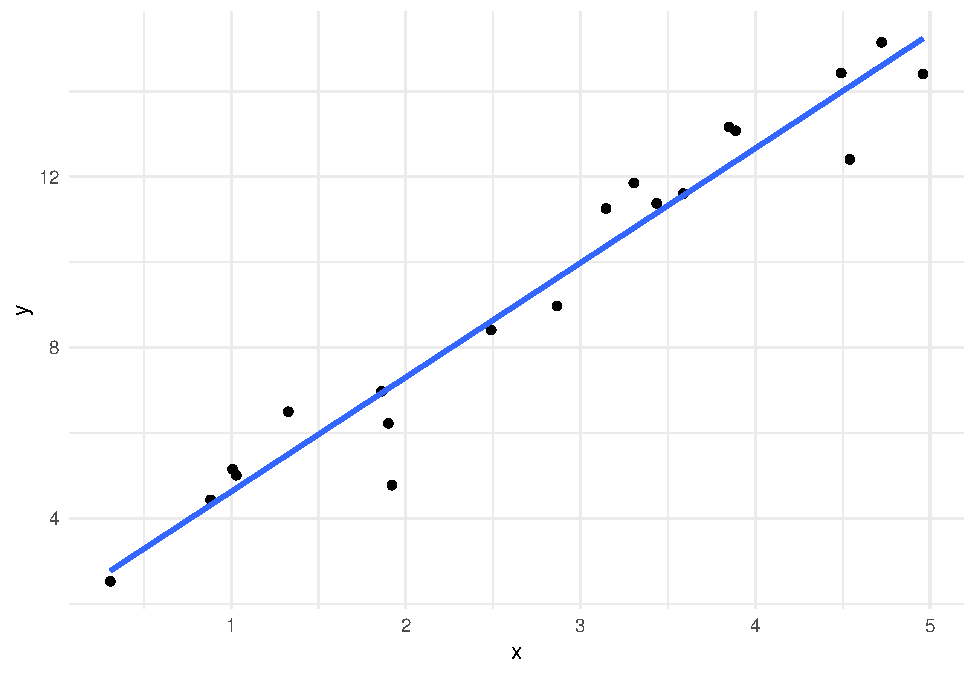
\includegraphics{rEkonometri_files/figure-latex/unnamed-chunk-152-1.pdf}

Her aykırı değerin kaldıraç etkisi yaratmadığını gösterelim.

\begin{Shaded}
\begin{Highlighting}[]
\NormalTok{y2 <-}\StringTok{ }\KeywordTok{c}\NormalTok{(y,}\DecValTok{18}\NormalTok{)}
\NormalTok{x2 <-}\StringTok{ }\KeywordTok{c}\NormalTok{(x,}\FloatTok{2.5}\NormalTok{)}
\NormalTok{df6 <-}\StringTok{ }\KeywordTok{data.frame}\NormalTok{(}\DataTypeTok{y=}\NormalTok{y2, }\DataTypeTok{x=}\NormalTok{x2)}
\NormalTok{model2 <-}\StringTok{ }\KeywordTok{lm}\NormalTok{(}\DataTypeTok{formula =}\NormalTok{ y }\OperatorTok{~}\StringTok{ }\NormalTok{x, }\DataTypeTok{data =}\NormalTok{ df6)}
\KeywordTok{summary}\NormalTok{(model2)}
\end{Highlighting}
\end{Shaded}

\begin{verbatim}
## 
## Call:
## lm(formula = y ~ x, data = df6)
## 
## Residuals:
##     Min      1Q  Median      3Q     Max 
## -2.8178 -0.8492 -0.2492  0.3396  8.8926 
## 
## Coefficients:
##             Estimate Std. Error t value Pr(>|t|)    
## (Intercept)   2.5610     1.1236   2.279   0.0344 *  
## x             2.6186     0.3648   7.179 8.06e-07 ***
## ---
## Signif. codes:  0 '***' 0.001 '**' 0.01 '*' 0.05 '.' 0.1 ' ' 1
## 
## Residual standard error: 2.277 on 19 degrees of freedom
## Multiple R-squared:  0.7306, Adjusted R-squared:  0.7164 
## F-statistic: 51.53 on 1 and 19 DF,  p-value: 8.056e-07
\end{verbatim}

\begin{Shaded}
\begin{Highlighting}[]
\KeywordTok{ggplot}\NormalTok{() }\OperatorTok{+}
\StringTok{  }\KeywordTok{geom_point}\NormalTok{(}\DataTypeTok{data =}\NormalTok{ df5, }\KeywordTok{aes}\NormalTok{(}\DataTypeTok{x =}\NormalTok{ x, }\DataTypeTok{y =}\NormalTok{ y), }\DataTypeTok{color =} \StringTok{"red"}\NormalTok{, }\DataTypeTok{size =} \DecValTok{3}\NormalTok{) }\OperatorTok{+}
\StringTok{  }\KeywordTok{geom_smooth}\NormalTok{(}\DataTypeTok{data =}\NormalTok{ df5, }\KeywordTok{aes}\NormalTok{(}\DataTypeTok{x =}\NormalTok{ x, }\DataTypeTok{y =}\NormalTok{ y), }\DataTypeTok{method =} \StringTok{"lm"}\NormalTok{, }\DataTypeTok{se =} \OtherTok{FALSE}\NormalTok{, }\DataTypeTok{color =} \StringTok{"red"}\NormalTok{) }\OperatorTok{+}
\StringTok{  }\KeywordTok{geom_point}\NormalTok{(}\DataTypeTok{data =}\NormalTok{ df6, }\KeywordTok{aes}\NormalTok{(}\DataTypeTok{x =}\NormalTok{ x, }\DataTypeTok{y =}\NormalTok{ y), }\DataTypeTok{color =} \StringTok{"blue"}\NormalTok{) }\OperatorTok{+}
\StringTok{  }\KeywordTok{geom_smooth}\NormalTok{(}\DataTypeTok{data =}\NormalTok{ df6, }\KeywordTok{aes}\NormalTok{(}\DataTypeTok{x =}\NormalTok{ x, }\DataTypeTok{y =}\NormalTok{ y), }\DataTypeTok{method =} \StringTok{"lm"}\NormalTok{, }\DataTypeTok{se =} \OtherTok{FALSE}\NormalTok{, }\DataTypeTok{color =} \StringTok{"blue"}\NormalTok{) }\OperatorTok{+}
\StringTok{  }\KeywordTok{theme_minimal}\NormalTok{()}
\end{Highlighting}
\end{Shaded}

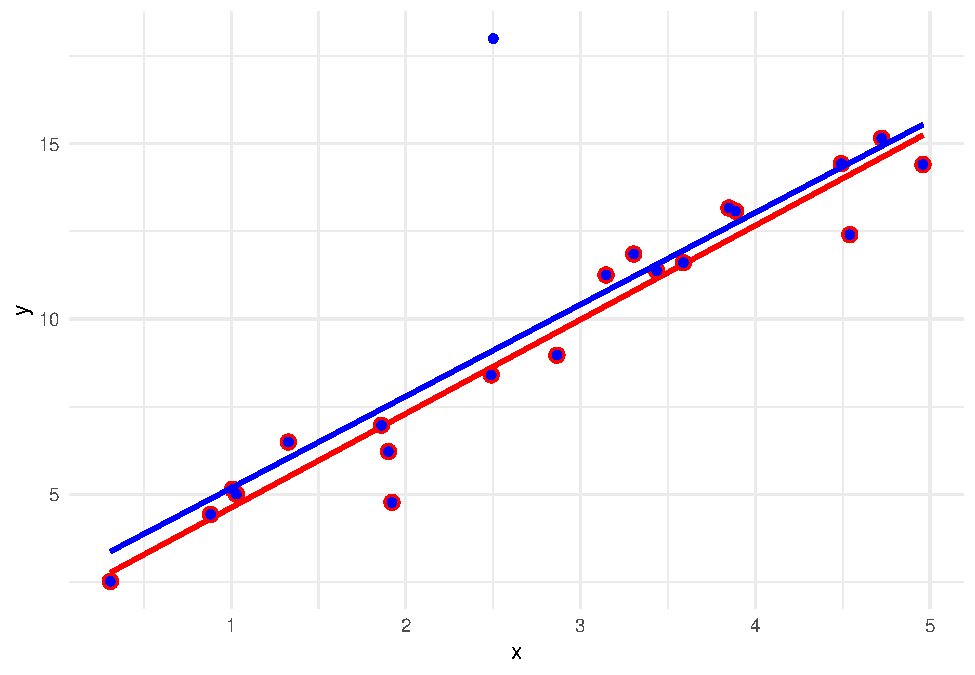
\includegraphics{rEkonometri_files/figure-latex/unnamed-chunk-154-1.pdf}

Eklediğimiz aykırı değer \(β_0\)'da etkiye neden oldu fakat \(β_1\)'de onun kadar bir etki göstermedi.

Yüksek kaldıraç etkisi olan ama baskın nokta olmayan bir gözleme örnek verelim.

\begin{Shaded}
\begin{Highlighting}[]
\NormalTok{y3 <-}\StringTok{ }\KeywordTok{c}\NormalTok{(y,}\DecValTok{25}\NormalTok{)}
\NormalTok{x3 <-}\StringTok{ }\KeywordTok{c}\NormalTok{(x,}\DecValTok{8}\NormalTok{)}
\NormalTok{df7 <-}\StringTok{ }\KeywordTok{data.frame}\NormalTok{(}\DataTypeTok{y=}\NormalTok{y3, }\DataTypeTok{x=}\NormalTok{x3)}
\NormalTok{model3 <-}\StringTok{ }\KeywordTok{lm}\NormalTok{(}\DataTypeTok{formula =}\NormalTok{ y }\OperatorTok{~}\StringTok{ }\NormalTok{x, }\DataTypeTok{data =}\NormalTok{ df7)}
\KeywordTok{summary}\NormalTok{(model3)}
\end{Highlighting}
\end{Shaded}

\begin{verbatim}
## 
## Call:
## lm(formula = y ~ x, data = df7)
## 
## Residuals:
##     Min      1Q  Median      3Q     Max 
## -2.2597 -0.2156  0.1867  0.6765  1.1257 
## 
## Coefficients:
##             Estimate Std. Error t value Pr(>|t|)    
## (Intercept)   1.6453     0.4081   4.032 0.000713 ***
## x             2.8048     0.1167  24.043 1.09e-15 ***
## ---
## Signif. codes:  0 '***' 0.001 '**' 0.01 '*' 0.05 '.' 0.1 ' ' 1
## 
## Residual standard error: 0.9396 on 19 degrees of freedom
## Multiple R-squared:  0.9682, Adjusted R-squared:  0.9665 
## F-statistic:   578 on 1 and 19 DF,  p-value: 1.095e-15
\end{verbatim}

\begin{Shaded}
\begin{Highlighting}[]
\KeywordTok{ggplot}\NormalTok{() }\OperatorTok{+}
\StringTok{  }\KeywordTok{geom_point}\NormalTok{(}\DataTypeTok{data =}\NormalTok{ df5, }\KeywordTok{aes}\NormalTok{(}\DataTypeTok{x =}\NormalTok{ x, }\DataTypeTok{y =}\NormalTok{ y), }\DataTypeTok{color =} \StringTok{"red"}\NormalTok{, }\DataTypeTok{size =} \DecValTok{3}\NormalTok{) }\OperatorTok{+}
\StringTok{  }\KeywordTok{geom_smooth}\NormalTok{(}\DataTypeTok{data =}\NormalTok{ df5, }\KeywordTok{aes}\NormalTok{(}\DataTypeTok{x =}\NormalTok{ x, }\DataTypeTok{y =}\NormalTok{ y), }\DataTypeTok{method =} \StringTok{"lm"}\NormalTok{, }\DataTypeTok{se =} \OtherTok{FALSE}\NormalTok{, }\DataTypeTok{color =} \StringTok{"red"}\NormalTok{) }\OperatorTok{+}
\StringTok{  }\KeywordTok{geom_point}\NormalTok{(}\DataTypeTok{data =}\NormalTok{ df7, }\KeywordTok{aes}\NormalTok{(}\DataTypeTok{x =}\NormalTok{ x, }\DataTypeTok{y =}\NormalTok{ y), }\DataTypeTok{color =} \StringTok{"blue"}\NormalTok{) }\OperatorTok{+}
\StringTok{  }\KeywordTok{geom_smooth}\NormalTok{(}\DataTypeTok{data =}\NormalTok{ df7, }\KeywordTok{aes}\NormalTok{(}\DataTypeTok{x =}\NormalTok{ x, }\DataTypeTok{y =}\NormalTok{ y), }\DataTypeTok{method =} \StringTok{"lm"}\NormalTok{, }\DataTypeTok{se =} \OtherTok{FALSE}\NormalTok{, }\DataTypeTok{color =} \StringTok{"blue"}\NormalTok{) }\OperatorTok{+}
\StringTok{  }\KeywordTok{theme_minimal}\NormalTok{()}
\end{Highlighting}
\end{Shaded}

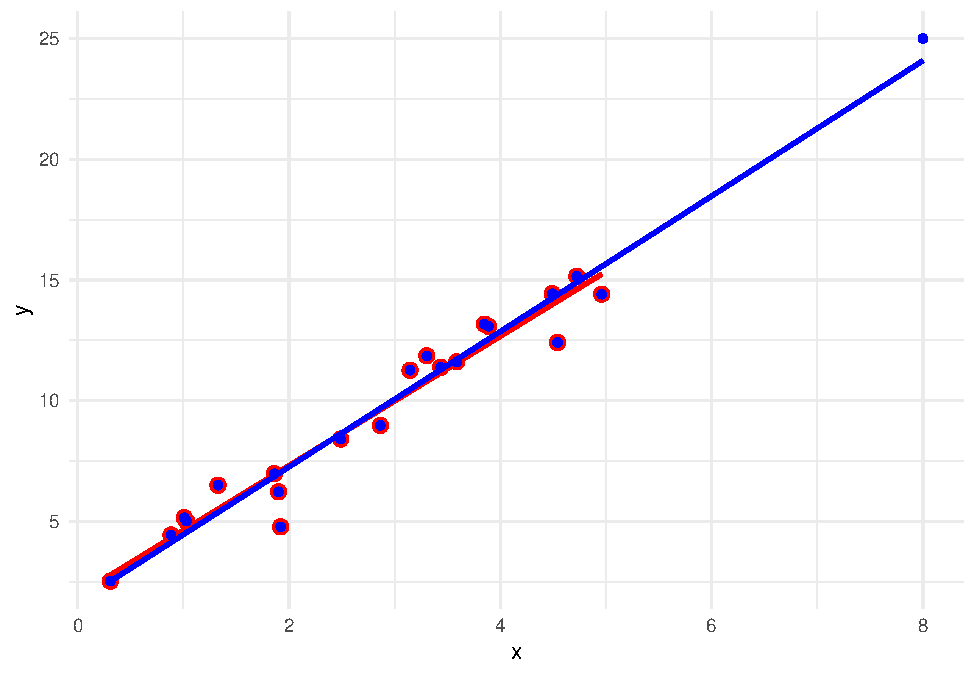
\includegraphics{rEkonometri_files/figure-latex/unnamed-chunk-156-1.pdf}

Kaldıraca sahip gözlem eğimi etkilemedi çünkü zaten doğrunun üzerinde. Böylece kaldıraç özelliğine sahip oldu ama baskın nokta olamadı.

Baskın nokta öyle değil böyle olur demek için son örneği görelim.

\begin{Shaded}
\begin{Highlighting}[]
\NormalTok{y4 <-}\StringTok{ }\KeywordTok{c}\NormalTok{(y,}\DecValTok{5}\NormalTok{)}
\NormalTok{x4 <-}\StringTok{ }\KeywordTok{c}\NormalTok{(x,}\DecValTok{8}\NormalTok{)}
\NormalTok{df8 <-}\StringTok{ }\KeywordTok{data.frame}\NormalTok{(}\DataTypeTok{y=}\NormalTok{y4, }\DataTypeTok{x=}\NormalTok{x4)}
\NormalTok{model4 <-}\StringTok{ }\KeywordTok{lm}\NormalTok{(}\DataTypeTok{formula =}\NormalTok{ y }\OperatorTok{~}\StringTok{ }\NormalTok{x, }\DataTypeTok{data =}\NormalTok{ df8)}
\KeywordTok{summary}\NormalTok{(model4)}
\end{Highlighting}
\end{Shaded}

\begin{verbatim}
## 
## Call:
## lm(formula = y ~ x, data = df8)
## 
## Residuals:
##      Min       1Q   Median       3Q      Max 
## -10.5000  -1.5247  -0.0009   2.3244   3.8185 
## 
## Coefficients:
##             Estimate Std. Error t value Pr(>|t|)   
## (Intercept)   5.3320     1.4385   3.707  0.00150 **
## x             1.2710     0.4112   3.091  0.00602 **
## ---
## Signif. codes:  0 '***' 0.001 '**' 0.01 '*' 0.05 '.' 0.1 ' ' 1
## 
## Residual standard error: 3.312 on 19 degrees of freedom
## Multiple R-squared:  0.3346, Adjusted R-squared:  0.2995 
## F-statistic: 9.553 on 1 and 19 DF,  p-value: 0.006017
\end{verbatim}

\begin{Shaded}
\begin{Highlighting}[]
\KeywordTok{ggplot}\NormalTok{() }\OperatorTok{+}
\StringTok{  }\KeywordTok{geom_point}\NormalTok{(}\DataTypeTok{data =}\NormalTok{ df5, }\KeywordTok{aes}\NormalTok{(}\DataTypeTok{x =}\NormalTok{ x, }\DataTypeTok{y =}\NormalTok{ y), }\DataTypeTok{color =} \StringTok{"red"}\NormalTok{, }\DataTypeTok{size =} \DecValTok{3}\NormalTok{) }\OperatorTok{+}
\StringTok{  }\KeywordTok{geom_smooth}\NormalTok{(}\DataTypeTok{data =}\NormalTok{ df5, }\KeywordTok{aes}\NormalTok{(}\DataTypeTok{x =}\NormalTok{ x, }\DataTypeTok{y =}\NormalTok{ y), }\DataTypeTok{method =} \StringTok{"lm"}\NormalTok{, }\DataTypeTok{se =} \OtherTok{FALSE}\NormalTok{, }\DataTypeTok{color =} \StringTok{"red"}\NormalTok{) }\OperatorTok{+}
\StringTok{  }\KeywordTok{geom_point}\NormalTok{(}\DataTypeTok{data =}\NormalTok{ df8, }\KeywordTok{aes}\NormalTok{(}\DataTypeTok{x =}\NormalTok{ x, }\DataTypeTok{y =}\NormalTok{ y), }\DataTypeTok{color =} \StringTok{"blue"}\NormalTok{) }\OperatorTok{+}
\StringTok{  }\KeywordTok{geom_smooth}\NormalTok{(}\DataTypeTok{data =}\NormalTok{ df8, }\KeywordTok{aes}\NormalTok{(}\DataTypeTok{x =}\NormalTok{ x, }\DataTypeTok{y =}\NormalTok{ y), }\DataTypeTok{method =} \StringTok{"lm"}\NormalTok{, }\DataTypeTok{se =} \OtherTok{FALSE}\NormalTok{, }\DataTypeTok{color =} \StringTok{"blue"}\NormalTok{) }\OperatorTok{+}
\StringTok{  }\KeywordTok{theme_minimal}\NormalTok{()}
\end{Highlighting}
\end{Shaded}

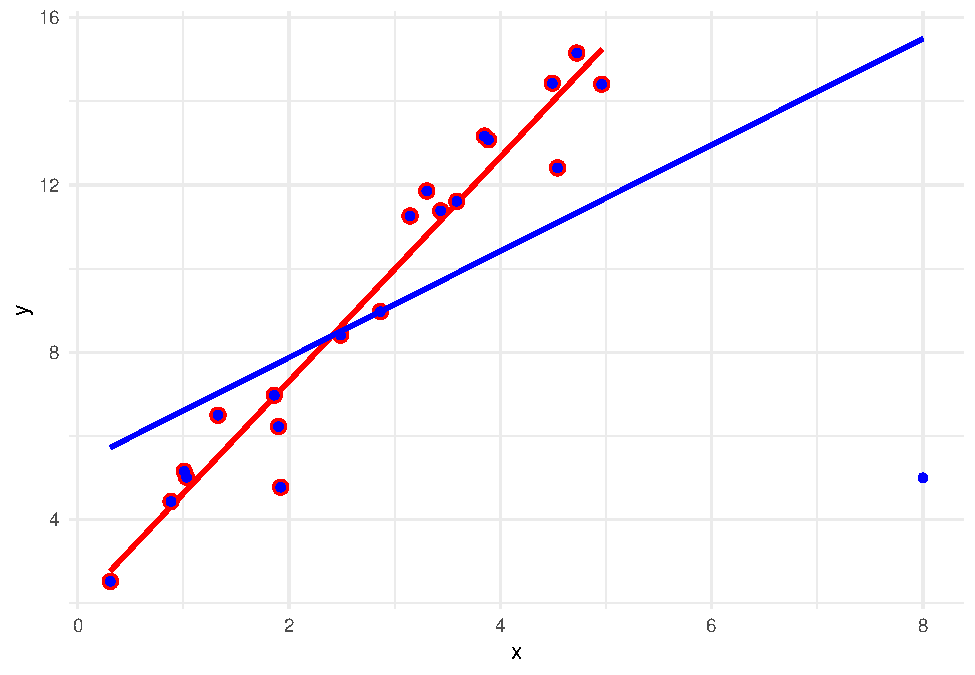
\includegraphics{rEkonometri_files/figure-latex/unnamed-chunk-158-1.pdf}

Eğimi oldukça değiştirdi ve baskın nokta özelliği kazandı.

\hypertarget{hata-teriminin-olasux131lux131k-daux11fux131lux131mux131}{%
\section{Hata Teriminin Olasılık Dağılımı}\label{hata-teriminin-olasux131lux131k-daux11fux131lux131mux131}}

Klasik doğrusal regresyon modelinin varsayımlarından biri modeldeki hata teriminin normal dağıldığı yönündedir. Eğer örneklem büyüklüğü nispeten küçükse varsayım oldukça önem kazanır çünkü t ve F testleri normallik varsayımına dayanır.

Biz daha önce Jarque-Bera (J-B) testinden bahsetmiştik. J-B, normallik testlerinden bir tanesidir ve büyük örneklemlerde çalışır (küçük örneklemlerde yanıltıcı olabilir). Daha önce formülünü görmemiştik ama şimdi öğrenelim: \(n * [\frac{S^2}{6} + \frac{(K-3)^2}{24}]\sim\chi^2_2\). Burada, n örneklem sayısı, S skewness ya da çarpıklık, K kurtosis ya da basıklıktır. Normal dağılım için S = 0 ve K = 3'tür. Bu değerler sağlandığında J-B = 0 olur. Bu da J-B'nin sıfıra yaklaştıkça normallik varsayımını güçlendirdiğini söyler. Ama biz ek olarak J-B'nin istatistiksel anlamlılığını bulmak isteriz ve bunun için de \(\chi^2\) dağılımını kullanırız. Karar verme aşamasında şuna bakacağız: Eğer J-B istatistiği ya da \(\chi^2\) istatistiği, örneğin \%5 seviyesinde, kritik \(\chi^2\) değerini aşarsa \(H_0\)'ı reddederiz. \(H_0\) hata teriminin normal dağıldığını varsayar. Uygulamada gerçek hata terimini kullanamadığımız için kalıntıyı (hata teriminin temsili) kullanırız.

\hypertarget{doux11frusal-olasux131lux131k-logit-ve-probit-modeller}{%
\chapter{Doğrusal Olasılık, Logit ve Probit Modeller}\label{doux11frusal-olasux131lux131k-logit-ve-probit-modeller}}

Yalnızca Cumhur İttifakı ve Millet İttifakı gibi iki grubun olduğunu varsayalım. Burada bağımlı değişken iki siyasal grup arasında seçimdir. Oy, Cumhur'a verilmişse Y = 1, Millet'e verilmişse Y = 0 diyelim. Ek olarak oy tercihlerini etkileyecek bazı bağımsız değişkenler de olacaktır (Oy vermede sizin tarafınızda neler etkili ise onları düşünebilirsiniz). Dikkat etmemiz gereken yer bağımlı değişken niteldir. Yani, bağımlı değişken ya öyledir ya da böyle.

Tabi ki tepki değişkenimizi iki şıklı değişkenlerle sınırlamak zorunda değiliz. Yukarıdaki varsayımı bozup üç gruba da çıkarabilirdik. Yani, çok şıklı tepki değişkenlerimiz olabilir.

Y bağımlı değişkeninin nicel olduğu bir regresyon modeli ile nitel olduğu bir regresyon modeli arasında nasıl bir fark vardır?

Kısa cevap: Biri nicel diğeri niteldir.

Uzun cevap: Y bağımlı değişkeninin nicel olduğu bir modelde amacımız Y'nin beklenen ya da ortalama değerini bulmaktır. Fakat Y bağımlı değişkeninin nitel olduğu bir modelde bir olayın gerçekleşme olasılığına odaklanırız. Millet İttifakı'na oy verme olasılığı gibi.

İki şıklı varsayımımız devam ediyor\ldots{}

İki şıklı bir tepki değişkeni için olasılık modelleri:

\begin{enumerate}
\def\labelenumi{\roman{enumi}.}
\item
  Doğrusal olasılık modeli
\item
  Logit modeli
\item
  Probit modeli
\item
  Tobit modeli
\end{enumerate}

\hypertarget{doux11frusal-olasux131lux131k}{%
\section{Doğrusal Olasılık}\label{doux11frusal-olasux131lux131k}}

Bildiğimiz model üzerinden gidelim: \(Y_i = \beta_1 + \beta_2X_i + \epsilon_i\)

X = aile geliri, Y = aile ev sahibi ise 1; değilse 0 olsun. Bu bildiğimiz doğrusal regresyon modeli değil mi? Fakat bağımlı değişken Y ikili olduğu için bu, doğrusal olasılık modeli adını alacaktır.

\(Y_i\) = 1 olma (olayın gerçekleşmesi) olasılığına \(P_i\), \(Y_i\) = 0 olma (olayın gerçekleşmemesi) olasılığına 1 -- \(P_i\) dersek; \(Y_i\) bernoulli olasılık dağılımına uyar. Bu arada n tane bağımsız deneme varsa, her birinin başarı olasılığı P, başarısızlık olasılığı 1-P ise ve bu denemelerden x tanesi başarılıysa, x'in binom dağılıma uyduğu söylenebilir.

Kısaca şunları bilmekte fayda olacaktır:

\begin{enumerate}
\def\labelenumi{\roman{enumi}.}
\item
  Doğrusal olasılık modelleri için \(u_i\)'lerin normal dağıldığını söyleyemeyiz. Çünkü, \(\epsilon_i\)'ler de \(Y_i\)'ler gibi ikili değer alır. Yani, bernoulli dağılımına uyar.
\item
  \(\epsilon_i\)'lerin sabit varyanslı oldukları ileri sürülemez. Yani, doğrusal olasılık modellerinde hata teriminin varyansı değişkendir.
\item
  \(\hat{Y_i}\)'nin 0 ile 1 arasında olup olmadığını anlamanın iki yolu:
\end{enumerate}

\begin{itemize}
\item
  Doğrusal olasılık modeli Sıradan En Küçük Kareler yöntemi ile tahmin edilip \(\hat{Y_i}\)'nin 0 ile 1 arasında olup olmadığına bakılır. Eğer bazıları 0'dan küçükse \(\hat{Y_i}\) 0; 1'den büyükse 1 sayılır.
\item
  Logit ve probit modelleri tahmin edilen olasılıkların 0 ile 1 mantıksal sınırları içinde kalmasını sağlar.
\end{itemize}

\begin{enumerate}
\def\labelenumi{\roman{enumi}.}
\setcounter{enumi}{3}
\tightlist
\item
  \(R^2\)'nin yararı sınırlıdır. Bu nedenle, bu istatistiğin kullanılmasından kaçınılması gerektiği ileri sürülür.
\end{enumerate}

\begin{Shaded}
\begin{Highlighting}[]
\KeywordTok{library}\NormalTok{(readxl);}\KeywordTok{library}\NormalTok{(tidyverse);}\KeywordTok{library}\NormalTok{(magrittr)}

\KeywordTok{setwd}\NormalTok{(}\StringTok{"C:/Users/datanerd/Desktop/Github/rEkonometri/data"}\NormalTok{)}
\NormalTok{df1 <-}\StringTok{ }\KeywordTok{read.table}\NormalTok{(}\DataTypeTok{file =} \StringTok{"http://www.econometrics.com/comdata/gujarati/data_15.1.shd"}\NormalTok{, }\DataTypeTok{sep =} \StringTok{""}\NormalTok{, }\DataTypeTok{header =} \OtherTok{FALSE}\NormalTok{, }\DataTypeTok{col.names =} \KeywordTok{c}\NormalTok{(}\StringTok{"y"}\NormalTok{,}\StringTok{"x"}\NormalTok{))}
\NormalTok{df2 <-}\StringTok{ }\KeywordTok{read_excel}\NormalTok{(}\StringTok{"Table8_1.xls"}\NormalTok{)}
\end{Highlighting}
\end{Shaded}

\begin{Shaded}
\begin{Highlighting}[]
\KeywordTok{str}\NormalTok{(df1)}
\end{Highlighting}
\end{Shaded}

\begin{verbatim}
## 'data.frame':    40 obs. of  2 variables:
##  $ y: int  0 1 1 0 0 1 1 0 0 0 ...
##  $ x: int  8 16 18 11 12 19 20 13 9 10 ...
\end{verbatim}

40 aile için verileri inceleyelim.

Bağımlı değişken:

\begin{itemize}
\tightlist
\item
  \textbf{y:} Ev sahipliği (Ev sahibi ise 1 değilse 0)
\end{itemize}

Bağımsız değişken(ler):

\begin{itemize}
\tightlist
\item
  \textbf{x:} Aile geliri
\end{itemize}

Sıradan En Küçük Kareler yöntemi ile tahmin edelim.

\begin{Shaded}
\begin{Highlighting}[]
\NormalTok{model <-}\StringTok{ }\KeywordTok{lm}\NormalTok{(}\DataTypeTok{formula =}\NormalTok{ y }\OperatorTok{~}\StringTok{ }\NormalTok{x, }\DataTypeTok{data =}\NormalTok{ df1)}
\KeywordTok{summary}\NormalTok{(model)}
\end{Highlighting}
\end{Shaded}

\begin{verbatim}
## 
## Call:
## lm(formula = y ~ x, data = df1)
## 
## Residuals:
##     Min      1Q  Median      3Q     Max 
## -0.4842 -0.1777  0.0052  0.2095  0.3329 
## 
## Coefficients:
##             Estimate Std. Error t value Pr(>|t|)    
## (Intercept) -0.94569    0.12284  -7.698 2.85e-09 ***
## x            0.10213    0.00816  12.515 4.73e-15 ***
## ---
## Signif. codes:  0 '***' 0.001 '**' 0.01 '*' 0.05 '.' 0.1 ' ' 1
## 
## Residual standard error: 0.2264 on 38 degrees of freedom
## Multiple R-squared:  0.8048, Adjusted R-squared:  0.7996 
## F-statistic: 156.6 on 1 and 38 DF,  p-value: 4.726e-15
\end{verbatim}

-0.94569 kesme terimi, sıfır gelirli bir ailenin ev sahibi olma olasılığını verir. Fakat değer eksi olmayacağı için bu değeri sıfırmış gibi görürüz.

0.10213 eğim değeriyse gelirdeki 1 birimlik artışın (örnekte 1000 \$), ev sahibi olma olasılığını ortalama olarak 0.10213 ya da \textasciitilde{} \%10 artıracağı anlamına gelir.

Örneğin, aile geliri 15 (15000) ise ev sahibi olma olasılığı aşağıdaki gibidir:

\begin{Shaded}
\begin{Highlighting}[]
\NormalTok{model}\OperatorTok{$}\NormalTok{coefficients[}\DecValTok{1}\NormalTok{] }\OperatorTok{+}\StringTok{ }\NormalTok{model}\OperatorTok{$}\NormalTok{coefficients[}\DecValTok{2}\NormalTok{] }\OperatorTok{*}\StringTok{ }\DecValTok{15}
\end{Highlighting}
\end{Shaded}

\begin{verbatim}
## (Intercept) 
##   0.5862786
\end{verbatim}

Aslında bize şu özellikleri taşıyan bir olasılık modeli gerekiyor:

\begin{enumerate}
\def\labelenumi{\roman{enumi})}
\item
  \(X_i\) arttıkça \(P_i\) de artar ama 0-1 aralığı dışına hiç çıkmaz
\item
  \(P_i\) ile \(X_i\) arasındaki ilişki doğrusal değildir (\(X_i\) küçüldükçe \(P_i\) gitgide daha yavaş 0'a yaklaşır; \(X_i\) çok büyük değerlere çıktıkça \(P_i\) gitgide daha yavaş 1'e yaklaşır).
\end{enumerate}

Bir uygulama daha yapıp ABD'li 1196 erkeğe ait rassal bir örneklemi inceleyelim.

\begin{Shaded}
\begin{Highlighting}[]
\NormalTok{df2 }\OperatorTok\StringTok{ }
\StringTok{  }\NormalTok{dplyr}\OperatorTok{::}\KeywordTok{select}\NormalTok{(}\KeywordTok{c}\NormalTok{(}\DecValTok{6}\NormalTok{,}\DecValTok{1}\NormalTok{,}\DecValTok{2}\NormalTok{,}\DecValTok{3}\NormalTok{,}\DecValTok{4}\NormalTok{))}

\KeywordTok{str}\NormalTok{(df2)}
\end{Highlighting}
\end{Shaded}

\begin{verbatim}
## tibble [1,196 x 5] (S3: tbl_df/tbl/data.frame)
##  $ smoker : num [1:1196] 0 1 0 0 1 0 0 1 0 1 ...
##  $ educ   : num [1:1196] 12 15 10 12 12 15 12 13.5 0 12 ...
##  $ age    : num [1:1196] 21 28 67 20 32 46 58 27 83 24 ...
##  $ income : num [1:1196] 8500 12500 12500 12500 20000 30000 30000 30000 6500 20000 ...
##  $ pcigs79: num [1:1196] 60.6 60.6 60.6 60.6 60.6 ...
\end{verbatim}

Bağımlı değişken:

\begin{itemize}
\tightlist
\item
  \textbf{smoker:} Sigara içiyorsa 1; içmiyorsa 0
\end{itemize}

Bağımsız değişken(ler):

\begin{itemize}
\item
  \textbf{educ:} Eğitim süresi
\item
  \textbf{age:} Yaş
\item
  \textbf{income:} Aile geliri
\item
  \textbf{pcigs79:} Eyaletteki sigaranın 1979 yılındaki fiyatları
\end{itemize}

Bağımsız değişken değerleri (educ, age, income, pcigs79) verildiğinde bağımlı değişkenin (smoker) koşullu beklentisi, sigara içme olayının gerçekleşmesinin koşullu olasılığı olarak yorumlanabilir.

\begin{Shaded}
\begin{Highlighting}[]
\NormalTok{model <-}\StringTok{ }\KeywordTok{lm}\NormalTok{(}\DataTypeTok{formula =}\NormalTok{ smoker }\OperatorTok{~}\NormalTok{., }\DataTypeTok{data =}\NormalTok{ df2)}
\KeywordTok{summary}\NormalTok{(model)}
\end{Highlighting}
\end{Shaded}

\begin{verbatim}
## 
## Call:
## lm(formula = smoker ~ ., data = df2)
## 
## Residuals:
##     Min      1Q  Median      3Q     Max 
## -0.6417 -0.3880 -0.2782  0.5563  0.8405 
## 
## Coefficients:
##               Estimate Std. Error t value Pr(>|t|)    
## (Intercept)  1.123e+00  1.884e-01   5.963 3.27e-09 ***
## educ        -2.061e-02  4.616e-03  -4.465 8.76e-06 ***
## age         -4.726e-03  8.290e-04  -5.701 1.50e-08 ***
## income       1.026e-06  1.632e-06   0.629   0.5298    
## pcigs79     -5.132e-03  2.852e-03  -1.799   0.0723 .  
## ---
## Signif. codes:  0 '***' 0.001 '**' 0.01 '*' 0.05 '.' 0.1 ' ' 1
## 
## Residual standard error: 0.477 on 1191 degrees of freedom
## Multiple R-squared:  0.03877,    Adjusted R-squared:  0.03554 
## F-statistic: 12.01 on 4 and 1191 DF,  p-value: 1.431e-09
\end{verbatim}

En az \%10 anlamlılık düzeyinde income hariç bütün değişkenler tek başına istatistiksel olarak anlamlıdır.

age, educ ve pcigs79 değişkenlerinin smoker üzerine negatif etkisi vardır.

Bağımsız değişkenler toplu halde anlamlıdır çünkü F değerinin neredeyse sıfıra yakın bir p değeri vardır.

Diğer tüm değişkenleri sabit tuttuğumuzda;

Muhtemelen sigara içmenin sağlık üzerindeki olumsuz etkisine bağlı olarak kişinin yaşı ilerledikçe sigara içme olasılığı yaklaşık olarak 0.005 oranında azalmaktadır (age).

Eğitimin 1 yıl artması sigara içme olasılığını 0.02 kadar azaltmaktadır (educ).

Sigara fiyatı 1 \$ yükseldiğinde sigara içme olasılığı yaklaşık olarak 0.005 kadar azalmaktadır (pcigs79).

0.038 olan \(R^2\) değeri çok düşüktür fakat bununla ilgili yukarıda yararının sınırlı olduğunu söylemiştik. Çünkü bağımlı değişken sadece 0-1 değerlerini alan bir nominal değişkendir.

Doğrusal olasılık modeli bizi yine de tatmin etmeyecek. Çünkü;

\begin{enumerate}
\def\labelenumi{\roman{enumi}.}
\item
  Doğrusal olasılık modeli sigara içme olasılığının bağımsız değişken değeriyle doğrusal hareket ettiğini varsayar.
\item
  Mantıken olasılık değeri 0-1 arasında yer alır ama doğrusal olasılık modelinde 0-1 dışına çıkabilir. Çünkü Sıradan En Küçük Kareler yöntemi bunu umursamaz.
\item
  Bağımlı değişken 0-1 değerlerini aldığından hata terimi için normal dağılım varsayımı geçerli olmaz.
\item
  Doğrusal olasılık modelindeki hata terimi değişen varyanslı olup, geleneksel anlamlılık testlerini şüpheli hale getirir.
\end{enumerate}

\hypertarget{logit-modeli}{%
\section{Logit Modeli}\label{logit-modeli}}

\(L_i = ln(\frac{P_i}{1-P_i}) = Z_i = \beta_1 + \beta_2X_i\)

Yukarıda yazılan model doğal logaritma alınarak oluşturulmuştur.

Logit modelinin özellikleri şöyledir:

\begin{enumerate}
\def\labelenumi{\roman{enumi}.}
\item
  P, 0'dan 1'e giderken (\(Z_i\), \(-\infty\)'dan \(+\infty\)'a doğru değişirken), logit (L) de \(-\infty\)'dan \(+\infty\)'a doğru değişir. Yani olasılıklar 0 ile 1 arasında yer alırken logitler böyle sınırlı değildir.
\item
  L, X'e göre doğrusal olmakla birlikte olasılıkların kendileri böyle değildir. Yani, olasılıkların X ile birlikte doğrusal olarak arttığı doğrusal olasılık modeli ile zıttır.
\item
  Tek bir bağımsız değişken değil; birden fazla bağımsız değişken de modele eklenebilir. Yani, birden fazla X.
\item
  Ev sahibi olma olasılığı \(P_i\) idi. O zaman ev sahibi olmama olasılığı \(1-P_i\) olmaz mı? Bu durumda \(\frac{P_i}{(1-P_i)}\) ev sahibi olmanın bahis oranı olur. Eğer logit L artıysa, bağımsız değişkenlerin değeri arttıkça, bağımlı değişkenin 1 olmasının bahis oranı yükselir; eğer logit L eksiyse, X büyüdükçe bağımlı değişkenin 1 olmasının bahis oranı düşer.
\item
  \(\beta_2\) eğimi, X'teki 1 birim değişmeye karşılık L'deki değişmeyi ölçer. Örneğin, gelir 1000 \$ değiştiğinde ev sahibi olmanın log-bahis oranının nasıl değiştiğini bildirir.
\item
  Kesme terimi \(\beta_1\) ise gelir sıfır olursa, ev sahibi olmanın log-bahis oranı değeridir.
\item
  Eğer belli bir değeri almadan ev sahibi olmanın kendi olasılığını tahmin etmek istersek, \(\beta_1\) ile \(\beta_2\) tahminleri bir kez elde edildikten sonra bunu \(P_i = \frac{e^z}{(1 + e^z)}\) ile bulabiliriz.
\item
  Bir önceki konuda adı geçen doğrusal olasılık modeli \(P_i\)'nin \(X_i\) ile doğrusal ilişki içinde olduğunu varsayarken, logit modeli log-bahis oranının \(X_i\) ile doğrusal ilişki içinde olduğunu varsayar.
\end{enumerate}

\(L_i = ln(\frac{P_i}{1-P_i}) = Z_i = \beta_1 + \beta_2X_i + u_i\)

Yazdığımız modeli tahmin etmek için \(X_i\)'den başka, bağımlı değişkenin ya da logit \(L_i\)'nin değerine gerek vardır. Bu da çözümleme için eldeki verinin türüne bağlıdır. İki tür veri ayırt ediyoruz: i) Tekil ya da mikro düzeydeki veri, ii) Gruplanmış veri ya da yinelenmiş veri.

Modeli kuralım. Model kurarken en çok olabilirlik yönteminden yararlanacağız.

\begin{Shaded}
\begin{Highlighting}[]
\NormalTok{logitmodel <-}\StringTok{ }\KeywordTok{glm}\NormalTok{(smoker }\OperatorTok{~}\StringTok{ }\NormalTok{educ }\OperatorTok{+}\StringTok{ }\NormalTok{age }\OperatorTok{+}\StringTok{ }\NormalTok{income }\OperatorTok{+}\StringTok{ }\NormalTok{pcigs79, }\DataTypeTok{family =} \KeywordTok{binomial}\NormalTok{(}\DataTypeTok{link =} \StringTok{"logit"}\NormalTok{), }\DataTypeTok{data =}\NormalTok{ df2)}
\KeywordTok{summary}\NormalTok{(logitmodel)}
\end{Highlighting}
\end{Shaded}

\begin{verbatim}
## 
## Call:
## glm(formula = smoker ~ educ + age + income + pcigs79, family = binomial(link = "logit"), 
##     data = df2)
## 
## Deviance Residuals: 
##     Min       1Q   Median       3Q      Max  
## -1.4608  -0.9829  -0.8055   1.2769   1.8384  
## 
## Coefficients:
##               Estimate Std. Error z value Pr(>|z|)    
## (Intercept)  2.745e+00  8.292e-01   3.311 0.000931 ***
## educ        -9.097e-02  2.067e-02  -4.402 1.07e-05 ***
## age         -2.085e-02  3.739e-03  -5.577 2.44e-08 ***
## income       4.720e-06  7.170e-06   0.658 0.510356    
## pcigs79     -2.232e-02  1.247e-02  -1.789 0.073538 .  
## ---
## Signif. codes:  0 '***' 0.001 '**' 0.01 '*' 0.05 '.' 0.1 ' ' 1
## 
## (Dispersion parameter for binomial family taken to be 1)
## 
##     Null deviance: 1588.9  on 1195  degrees of freedom
## Residual deviance: 1541.7  on 1191  degrees of freedom
## AIC: 1551.7
## 
## Number of Fisher Scoring iterations: 4
\end{verbatim}

educ ve age değişkenleri istatistiksel olarak oldukça anlamlıdır. İşaretler de negatiftir. Yani, insanların eğitimi ya da yaşı arttıkça sigara içme olasılıkları azalmaktadır.

pcigs79 değişkeni de \%7'de anlamlıdır. Yani, sigara fiyatı arttıkça sigara içme olasılığı düşer.

income istatistiksel olarak anlamlı değildir.

Diğer değişkenler sabit tutulduğunda;

Eğitimdeki bir yıllık artış ortalama logit değerini 0.09 azaltacaktır (educ). Yani, sigara içme lehine olan bahis oranının logaritması 0.09 azalacaktır. \(P_i\), sigara içme; \(1-P_i\) ise sigara içmeme olasılığı olsun. \(\frac{P_i}{1-P_i}\) basitçe sigara içme lehine olan bahis oranıdır.

Yaştaki bir yıllık artış ortalama logit değerini 0.02 azaltacaktır (age). Yani, sigara içme lehine olan bahis oranının logaritması 0.02 azalacaktır.

Sigara fiyatlarındaki 1 \$'lık artış ortalama logit değerini 0.02 azaltacaktır (pcigs79). Yani, sigara içme lehine olan bahis oranının logaritması 0.02 azalacaktır.

\(R^2\)'nin çok anlamlı olmayacağından bahsetmiştik. Fakat bunun yerine sayma \(R^2\) kullanabiliriz. Bu, doğru kestirim sayısının gözlem sayısına oranıdır. Eğer kestirilen değer 0.5'ten büyükse 1; küçükse 0 değerini alır. Bu durumda sayma \(R^2\);

\begin{Shaded}
\begin{Highlighting}[]
\NormalTok{df2 }\OperatorTok\StringTok{ }
\StringTok{  }\KeywordTok{mutate}\NormalTok{(}\DataTypeTok{fitted =}\NormalTok{ logitmodel}\OperatorTok{$}\NormalTok{fitted.values) }\OperatorTok\StringTok{ }
\StringTok{  }\KeywordTok{mutate}\NormalTok{(}\DataTypeTok{tahmin =} \KeywordTok{ifelse}\NormalTok{(fitted }\OperatorTok{>}\StringTok{ }\FloatTok{0.5}\NormalTok{, }\DecValTok{1}\NormalTok{, }\DecValTok{0}\NormalTok{)) }\OperatorTok\StringTok{ }
\StringTok{  }\KeywordTok{mutate}\NormalTok{(}\DataTypeTok{durum =} \KeywordTok{ifelse}\NormalTok{(smoker }\OperatorTok{==}\StringTok{ }\NormalTok{tahmin, }\StringTok{"başarılı"}\NormalTok{, }\StringTok{"başarısız"}\NormalTok{))}

\NormalTok{df2 }\OperatorTok\StringTok{ }
\StringTok{  }\KeywordTok{count}\NormalTok{(durum)}
\end{Highlighting}
\end{Shaded}

\begin{verbatim}
## # A tibble: 2 x 2
##   durum         n
##   <chr>     <int>
## 1 başarılı    730
## 2 başarısız   466
\end{verbatim}

Sayma \(R^2\) değeri 730 / 1196 = 0.6103679 ya da \%61 olacak.

Bizim önceliğimiz regresyon katsayılarının beklenen işaretleri ile istatistiksel anlamlılıkları olacaktır.

Doğrusal olasılık modelinde hata terimi normal olmayan dağılımdaydı. Logit modelde ise hata terimi lojistik dağılıma sahiptir. Şimdi de hata terimi normal dağılımlı olan probit modeli göreceğiz.

\hypertarget{probit-model}{%
\section{Probit Model}\label{probit-model}}

\begin{Shaded}
\begin{Highlighting}[]
\NormalTok{probitmodel <-}\StringTok{ }\KeywordTok{glm}\NormalTok{(smoker }\OperatorTok{~}\StringTok{ }\NormalTok{educ }\OperatorTok{+}\StringTok{ }\NormalTok{age }\OperatorTok{+}\StringTok{ }\NormalTok{income }\OperatorTok{+}\StringTok{ }\NormalTok{pcigs79, }\DataTypeTok{family =} \KeywordTok{binomial}\NormalTok{(}\DataTypeTok{link =} \StringTok{"probit"}\NormalTok{), }\DataTypeTok{data =}\NormalTok{ df2)}
\KeywordTok{summary}\NormalTok{(probitmodel)}
\end{Highlighting}
\end{Shaded}

\begin{verbatim}
## 
## Call:
## glm(formula = smoker ~ educ + age + income + pcigs79, family = binomial(link = "probit"), 
##     data = df2)
## 
## Deviance Residuals: 
##     Min       1Q   Median       3Q      Max  
## -1.4607  -0.9830  -0.8028   1.2774   1.8546  
## 
## Coefficients:
##               Estimate Std. Error z value Pr(>|z|)    
## (Intercept)  1.702e+00  5.096e-01   3.339  0.00084 ***
## educ        -5.623e-02  1.262e-02  -4.456 8.35e-06 ***
## age         -1.297e-02  2.277e-03  -5.695 1.23e-08 ***
## income       2.720e-06  4.411e-06   0.617  0.53741    
## pcigs79     -1.379e-02  7.685e-03  -1.795  0.07268 .  
## ---
## Signif. codes:  0 '***' 0.001 '**' 0.01 '*' 0.05 '.' 0.1 ' ' 1
## 
## (Dispersion parameter for binomial family taken to be 1)
## 
##     Null deviance: 1588.9  on 1195  degrees of freedom
## Residual deviance: 1541.2  on 1191  degrees of freedom
## AIC: 1551.2
## 
## Number of Fisher Scoring iterations: 4
\end{verbatim}

Sonuçlar aslında logit model ile aynı (niceliksel farklılılar var tabi ki).

Gujarati şu notu düşer: \emph{Logit ve probit modelleri genellikle benzer sonuçlar verir. İki model arasındaki temel fark lojistik dağılımın biraz daha şişman kuyruklarının olmasıdır; lojistik dağılımlı rassal bir değişkenin varyansının yaklaşık} \(\frac{\pi^2}{3}\), \emph{oysa (standart) normal dağılımlı değişkeninkinin 1 olduğunu hatırlayalım. Yani, logitte} \(P_i\) \emph{koşullu olasılığı probitten daha düşük bir hızla 0 veya 1'e yaklaşır. Ancak uygulamada birisini diğerine tercih etmenin ikna edici bir nedeni bulunmamaktadır. Nispeten matematiksel kolaylığı sebebiyle araştırmacı logiti probite tercih etmektedir.} Çağlayan ve Güriş ise şuna dikkat çeker: \emph{Aralarındaki fark sadece kuyruklarda bulunmaktadır. Bu fark; logit eğrisinin daha kalın kuyruklu olması yani eksene probit eğrisinden daha geç yaklaşması şeklinde açıklanabilir. (\ldots) özellikle verinin kuyruklardaki yoğunluğuna konsantre olunmadıysa probit model mi logit model mi sorusunun önemi pek bulunmamaktadır.}

\hypertarget{uxe7ok-terimli-regresyon-modelleri}{%
\chapter{Çok Terimli Regresyon Modelleri}\label{uxe7ok-terimli-regresyon-modelleri}}

\begin{Shaded}
\begin{Highlighting}[]
\KeywordTok{library}\NormalTok{(readxl);}\KeywordTok{library}\NormalTok{(tidyverse);}\KeywordTok{library}\NormalTok{(magrittr);}\KeywordTok{library}\NormalTok{(nnet);}\KeywordTok{library}\NormalTok{(mlogit);}\KeywordTok{library}\NormalTok{(stargazer);}\KeywordTok{library}\NormalTok{(Epi)}

\KeywordTok{setwd}\NormalTok{(}\StringTok{"C:/Users/datanerd/Desktop/Github/rEkonometri/data"}\NormalTok{)}
\NormalTok{df1 <-}\StringTok{ }\KeywordTok{read_excel}\NormalTok{(}\StringTok{"Table9_1.xls"}\NormalTok{)}
\NormalTok{df2 <-}\StringTok{ }\KeywordTok{read_excel}\NormalTok{(}\StringTok{"Table9_3.xls"}\NormalTok{)}
\end{Highlighting}
\end{Shaded}

\hypertarget{uxe7ok-terimli-logit-model}{%
\section{Çok Terimli Logit Model}\label{uxe7ok-terimli-logit-model}}

Bağımlı değişkenin ikiden fazla seçenekli olduğu durumlar vardır. Ulaşım tercihleri (araba, metrobüs, metro), eğitim tercihi (lisans, yüksek lisans, doktora), anket cevapları (katılıyorum, kısmen, katılmıyorum) gibi. Bu tür modellere çok terimli regresyon modelleri denir.

Verdiğimiz örneklerde ulaşım ve eğitim tercihleri gibi örnekler nominal ya da sıralamasız çok terimli regresyon modelleri iken; anket cevapları gibi örnekler de sıralamalı çok terimli regresyon modelleridir.

\begin{Shaded}
\begin{Highlighting}[]
\KeywordTok{str}\NormalTok{(df1)}
\end{Highlighting}
\end{Shaded}

\begin{verbatim}
## tibble [1,000 x 8] (S3: tbl_df/tbl/data.frame)
##  $ psechoice: num [1:1000] 2 2 3 3 3 3 2 1 3 3 ...
##  $ hscath   : num [1:1000] 0 0 0 0 0 0 0 0 0 0 ...
##  $ grades   : num [1:1000] 9.08 8.31 7.42 7.42 7.42 ...
##  $ faminc   : num [1:1000] 62.5 42.5 62.5 62.5 62.5 12.5 30 42.5 17.5 42.5 ...
##  $ famsiz   : num [1:1000] 5 4 4 4 4 2 5 4 3 6 ...
##  $ parcoll  : num [1:1000] 0 0 0 0 0 0 0 0 0 0 ...
##  $ female   : num [1:1000] 0 1 1 1 1 1 0 0 1 0 ...
##  $ black    : num [1:1000] 0 0 0 0 0 0 0 0 0 0 ...
\end{verbatim}

Veriler 1000 lise mezununun üç seçenek arasından tercihleri ile alakalıdır. Bu üç seçeneğin olasılık toplamı 1'dir. Çünkü karşılıklı dışlayan ya da birlikte kapsayıcı olayların olasılıkları toplamı 1 yapar. Dolayısıyla herhangi iki seçeneğin olasılığı belirlendiğinde üçüncüsünün olasılığı ortaya çıkmış olacaktır.

Bu uygulama seçene ya da bireye özgü verilerdir. Seçimler seçimi yapanın özelliklerine bağlıdır. Bu tür veriler olduğunda çok terimli logit ya da çok terimli probit modeller ile tahmin edilir.

Bağımlı değişken:

\begin{itemize}
\tightlist
\item
  \textbf{psechoice:} Üniversite ile devam etmeme ise 1, 2 yıllık ise 2, 4 yıllık ise 3
\end{itemize}

Bağımsız değişken(ler):

\begin{itemize}
\item
  \textbf{hscath:} Katolik okul mezunu ise 1; değilse 0
\item
  \textbf{grades:} Matematik, ingilizce ve sosyal bilgiler ortalama puanıdır (1-13 arasında değer alır ve arttıkça zayıf performansı işaret eder)
\item
  \textbf{faminc:} Brüt aile geliri (1000\$)
\item
  \textbf{famsiz:} Ailedeki birey sayısı
\item
  \textbf{parcoll:} En çok eğitimli olan ebeveyn üniversite mezunu ya da daha yükseğine sahipse 1; değilse 0
\item
  \textbf{female:} Kadın ise 1; değilse 0
\item
  \textbf{black:} Siyah ise 1; değilse 0
\end{itemize}

\(\pi_{i1} = \frac{1}{(1 + e^{\alpha_2 + \beta_2X_i} + e^{\alpha_3 + \beta_3X_i})}\)

\(\pi_{i2} = \frac{e^{\alpha_2 + \beta_2X_i}}{(1 + e^{\alpha_2 + \beta_2X_i} + e^{\alpha_3 + \beta_3X_i})}\)

\(\pi_{i3} = \frac{e^{\alpha_3 + \beta_3X_i}}{(1 + e^{\alpha_2 + \beta_2X_i} + e^{\alpha_3 + \beta_3X_i})}\)

Modeli kuralım.

\begin{Shaded}
\begin{Highlighting}[]
\NormalTok{mlogitmodel <-}\StringTok{ }\KeywordTok{multinom}\NormalTok{(psechoice }\OperatorTok{~}\NormalTok{., }\DataTypeTok{data =}\NormalTok{ df1)}
\end{Highlighting}
\end{Shaded}

\begin{verbatim}
## # weights:  27 (16 variable)
## initial  value 1098.612289 
## iter  10 value 877.997257
## iter  20 value 829.888040
## iter  30 value 829.747004
## final  value 829.746599 
## converged
\end{verbatim}

\begin{Shaded}
\begin{Highlighting}[]
\KeywordTok{summary}\NormalTok{(mlogitmodel)}
\end{Highlighting}
\end{Shaded}

\begin{verbatim}
## Call:
## multinom(formula = psechoice ~ ., data = df1)
## 
## Coefficients:
##   (Intercept)    hscath     grades      faminc      famsiz  parcoll      female
## 2    2.268539 -3.038208 -0.2994902 0.009810147 -0.09708496 0.526391  0.14149231
## 3    5.007894 11.556727 -0.6982877 0.014857249 -0.06658362 1.024127 -0.05761971
##       black
## 2 0.5558017
## 3 1.4949591
## 
## Std. Errors:
##   (Intercept)       hscath     grades      faminc     famsiz   parcoll
## 2   0.5782259 1.977826e-08 0.05582942 0.004195157 0.07262562 0.2899024
## 3   0.5671101 9.205296e-07 0.05744761 0.004122069 0.07207269 0.2773820
##      female     black
## 2 0.1961625 0.4296691
## 3 0.1964270 0.4170274
## 
## Residual Deviance: 1659.493 
## AIC: 1691.493
\end{verbatim}

Burada default olarak üniversiteye gitmeme (1) seçilmiştir. Yani, baz kategori 1'dir. Ama bu model kurulmadan önce aşağıdaki gibi değiştirilebilir.

\begin{Shaded}
\begin{Highlighting}[]
\CommentTok{#df1$psechoice <- factor(df1$psechoice)}
\CommentTok{#df1$psechoice <- relevel(df1$psechoice, ref = 1)}
\end{Highlighting}
\end{Shaded}

Baz kategori değiştirilirse çıktıdaki parametreler değişir. Ama tercihlerin olasılıkları hep aynı kalır. Çıktıda yer alan 2 ve 3 şunu ifade etmektedir:

2: Okul tercihi 1 ile ilişkili olarak okul tercihi 2'nin logit tahminleri

3: Okul tercihi 1 ile ilişkili olarak okul tercihi 3'ün logit tahminleri

\begin{Shaded}
\begin{Highlighting}[]
\NormalTok{mlogitdata <-}\StringTok{ }\KeywordTok{mlogit.data}\NormalTok{(df1, }\DataTypeTok{choice=}\StringTok{"psechoice"}\NormalTok{, }\DataTypeTok{shape =} \StringTok{"wide"}\NormalTok{)}
\NormalTok{mlogitmodel <-}\StringTok{ }\KeywordTok{mlogit}\NormalTok{(psechoice }\OperatorTok{~}\StringTok{ }\DecValTok{1}\OperatorTok{|}\StringTok{ }\NormalTok{hscath }\OperatorTok{+}\StringTok{ }\NormalTok{grades }\OperatorTok{+}\StringTok{ }\NormalTok{faminc }\OperatorTok{+}\StringTok{ }\NormalTok{famsiz }\OperatorTok{+}\StringTok{ }\NormalTok{parcoll }\OperatorTok{+}\StringTok{ }\NormalTok{female }\OperatorTok{+}\StringTok{ }\NormalTok{black, }\DataTypeTok{data=}\NormalTok{mlogitdata)}

\KeywordTok{stargazer}\NormalTok{(mlogitmodel, }\DataTypeTok{type=}\StringTok{"text"}\NormalTok{)}
\end{Highlighting}
\end{Shaded}

\begin{verbatim}
## 
## ==========================================
##                    Dependent variable:    
##                ---------------------------
##                         psechoice         
## ------------------------------------------
## 2:(intercept)           2.269***          
##                          (0.578)          
##                                           
## 3:(intercept)           5.008***          
##                          (0.567)          
##                                           
## 2:hscath                 -1.023           
##                        (4,397.323)        
##                                           
## 3:hscath                 17.047           
##                        (3,026.810)        
##                                           
## 2:grades                -0.300***         
##                          (0.056)          
##                                           
## 3:grades                -0.698***         
##                          (0.057)          
##                                           
## 2:faminc                 0.010**          
##                          (0.004)          
##                                           
## 3:faminc                0.015***          
##                          (0.004)          
##                                           
## 2:famsiz                 -0.097           
##                          (0.073)          
##                                           
## 3:famsiz                 -0.067           
##                          (0.072)          
##                                           
## 2:parcoll                0.526*           
##                          (0.290)          
##                                           
## 3:parcoll               1.024***          
##                          (0.277)          
##                                           
## 2:female                  0.142           
##                          (0.196)          
##                                           
## 3:female                 -0.058           
##                          (0.196)          
##                                           
## 2:black                   0.556           
##                          (0.430)          
##                                           
## 3:black                 1.495***          
##                          (0.417)          
##                                           
## ------------------------------------------
## Observations              1,000           
## R2                        0.185           
## Log Likelihood          -829.747          
## LR Test           377.822*** (df = 16)    
## ==========================================
## Note:          *p<0.1; **p<0.05; ***p<0.01
\end{verbatim}

İlk olarak istatistiksel anlamlılıklara bakalım. 2 olanlarda grades, faminc, parcoll; 3 olanlarda grades, faminc, parcoll ve black değişkenleri istatistiksel olarak anlamlıdır.

Yapay \(R^2\) değeri 0.185 olarak bulunmuş. McFadden tarafından geliştirilen bu \(R^2 = 1 – (\frac{ln_{L_u}}{ln_{L_0}})\) olarak ifade edilir. Burada, \(L_u\) uyumu yapılmış modelin olabilirlik oranı iken; \(L_0\) modelin hiçbir açıklayıcı değişkeni olmaksızın olabilirlik oranıdır.

p değeri neredeyse sıfır olan ve 378 olarak tahmin edilen LR tahmini istatistiksel olarak oldukça anlamlıdır. Bu da bu modelin uyumunun iyi olduğunu belirtir (her ne kadar bütün eğim parametreleri istatistiksel olarak anlamlı olmasa da).

Yorumları farklı yollardan yapabiliriz.

1: üniversite ile devam etmeme, 2: 2 yıllık, 3: 4 yıllık.

Diğer tüm değişkenler sabit tutulduğunda;

Bir bağımsız değişkene ait pozitif parametre, tercih 1'e göre tercih 2 için artan bahis oranını belirtir. Bağımsız değişkene ait negatif parametre ise tercih 1'in lehine olan bahis oranının tercih 2'ye göre arttığı anlamına gelir. Çıktıya baktığımızda, pozitif parametreli olan aile geliri (faminc) arttığında tercih 1'e göre tercih 2 bahis oranı artacaktır. Ya da örneğin, negatif parametreli olan puanlar (grades) tercih 1 lehine olan bahis oranının tercih 2'den yüksek olduğunu gösterir. Ortalama puan (grades) 1 birim arttığında üniversiteyi tercih etmemeye göre 2 yıllık bir yeri tercih etmenin logaritmik olasılığı 0.2995 kadar düşer. Üniversiteye gitmemeye göre 2 yıllık bir yeri tercih etme lehine bahis oranı ise 0.7411 ya da \%74 (0.2995'in ters logaritması).

\begin{Shaded}
\begin{Highlighting}[]
\KeywordTok{exp}\NormalTok{(}\OperatorTok{-}\FloatTok{0.2995}\NormalTok{)}
\end{Highlighting}
\end{Shaded}

\begin{verbatim}
## [1] 0.7411887
\end{verbatim}

\hypertarget{koux15fullu-logit-model}{%
\section{Koşullu Logit Model}\label{koux15fullu-logit-model}}

Çok terimli logit modeller için seçimler seçimi yapanın özelliklerine bağlıdır demiştik. Koşullu logit modellerde ise seçime özgü nitelikler vardır. Yani, bireye ait özellikler bulunmamaktadır.

\begin{Shaded}
\begin{Highlighting}[]
\KeywordTok{str}\NormalTok{(df2)}
\end{Highlighting}
\end{Shaded}

\begin{verbatim}
## tibble [840 x 13] (S3: tbl_df/tbl/data.frame)
##  $ choice       : num [1:840] 0 0 0 1 0 0 0 1 0 0 ...
##  $ termtime     : num [1:840] 69 34 35 0 64 44 53 0 69 34 ...
##  $ invehiclecost: num [1:840] 59 31 25 10 58 31 25 11 115 98 ...
##  $ traveltime   : num [1:840] 100 372 417 180 68 354 399 255 125 892 ...
##  $ travelcost   : num [1:840] 70 71 70 30 68 84 85 50 129 195 ...
##  $ income       : num [1:840] 35 35 35 35 30 30 30 30 40 40 ...
##  $ partysize    : num [1:840] 1 1 1 1 2 2 2 2 1 1 ...
##  $ id           : num [1:840] 1 1 1 1 2 2 2 2 3 3 ...
##  $ mode         : chr [1:840] "air" "train" "bus" "car" ...
##  $ air          : num [1:840] 1 0 0 0 1 0 0 0 1 0 ...
##  $ train        : num [1:840] 0 1 0 0 0 1 0 0 0 1 ...
##  $ bus          : num [1:840] 0 0 1 0 0 0 1 0 0 0 ...
##  $ car          : num [1:840] 0 0 0 1 0 0 0 1 0 0 ...
\end{verbatim}

Veriler 210 yolcunun ulaşım tercihleri (hava, otobüs, araba, tren) ile alakalıdır.

Bağımlı değişken:

\begin{itemize}
\tightlist
\item
  \textbf{mode:} air (hava), bus (otobüs), car (araba), tren (train)
\end{itemize}

Bağımsız değişken(ler):

\begin{itemize}
\item
  \textbf{termtime:} Terminal bekleme süresi (araba için 0)
\item
  \textbf{invehiclecost:} Araç maliyeti
\item
  \textbf{traveltime:} Araçla seyahat süresi
\item
  \textbf{travelcost:} Araç maliyeti ile bireye ait zamanın alternatif maliyeti toplamı
\item
  \textbf{income:} Aile geliri
\item
  \textbf{partysize:} Seçilen yöntemdeki yolcu sayısı.
\end{itemize}

Ama koşullu logit modeller için seçime özgü nitelikler var demiştik fakat income ve partysize bireye özgü değişkenler? İşte bunları dahil etmeyeceğiz. Bunları karma modellerde dahil edeceğiz.

Veri setinin içinde one hot encoding yapılmış. Kısaca mesela, ilk satırda mode = air olduğu için air sütunu 1 diğerleri 0 olarak kodlanmıştır.

Çoklu logit modelde olduğu gibi koşullu logit modelde de bir ulaşım aracını baz alacağız. Bu, car olsun.

\begin{Shaded}
\begin{Highlighting}[]
\NormalTok{clogitmodel <-}\StringTok{ }\KeywordTok{clogistic}\NormalTok{(choice }\OperatorTok{~}\StringTok{ }\NormalTok{termtime }\OperatorTok{+}\StringTok{ }\NormalTok{invehiclecost }\OperatorTok{+}\StringTok{ }\NormalTok{traveltime }\OperatorTok{+}\StringTok{ }\NormalTok{travelcost }\OperatorTok{+}\StringTok{ }\NormalTok{air }\OperatorTok{+}\StringTok{ }\NormalTok{train }\OperatorTok{+}\StringTok{ }\NormalTok{bus, }\DataTypeTok{strata =}\NormalTok{ id, }\DataTypeTok{data =}\NormalTok{ df2)}
\NormalTok{clogitmodel}
\end{Highlighting}
\end{Shaded}

\begin{verbatim}
## 
## Call: 
## clogistic(formula = choice ~ termtime + invehiclecost + traveltime + 
##     travelcost + air + train + bus, strata = id, data = df2)
## 
## 
## 
## 
##                  coef exp(coef) se(coef)     z       p
## termtime      -0.1036     0.902  0.01094 -9.48 0.0e+00
## invehiclecost -0.0849     0.919  0.01938 -4.38 1.2e-05
## traveltime    -0.0133     0.987  0.00252 -5.30 1.2e-07
## travelcost     0.0693     1.072  0.01743  3.97 7.0e-05
## air            5.2047   182.133  0.90521  5.75 8.9e-09
## train          4.3606    78.304  0.51067  8.54 0.0e+00
## bus            3.7632    43.087  0.50626  7.43 1.1e-13
## 
## Likelihood ratio test=213  on 7 df, p=0, n=840
\end{verbatim}

p değerlerinin oldukça düşük olduğunu görüyoruz. Bu da parametrelerin istatistiksel olarak anlamlı olduklarını gösteriyor.

Likelihood ratio ya da olabilirlik oranı istatistiği 213 oldukça anlamlıdır. Bu, bütün eğim parametrelerinin aynı anda sıfıra eşit olduğu hipotezinin güçlü bir şekilde reddi anlamına gelir.

Diğer değişkenler sabit tutulduğunda;

termtime: Arabayla seyahate göre terminalde daha uzun bekleme süresi olan ulaşım türü daha az seçilme eğiliminde olacaktır. Herhangi bir ulaşım türü için terminal süresini 1 dakika artırmak bu türü kullanmanın bahis oranını \%10 kadar düşürür.

traveltime: Eğer arabaya göre bir ulaşım aracındaki seyahat süresi daha uzunsa bu ulaşım türü muhtemelen seçilmeyecektir. Herhangi bir ulaşım türü için seyahat süresini 1 dakika artırmak bu türü kullanmanın bahis oranını \%2 kadar düşürür.

travelcost: Arabaya göre daha düşük alternatif maliyeti olan ulaşım türü seçilecektir.

\hypertarget{karma-logit-model}{%
\section{Karma Logit Model}\label{karma-logit-model}}

Çok terimli logit modelde seçimler seçimi yapanın özelliklerine bağlıdır demiştik. Koşullu logit modelde ise seçime ait özellikler var olup bireye ait özellikler bulunmamaktadır demiştik. Şu anki başlığımız olan karma logit modelde her ikisini de modele dahil edebiliriz.

Karma logit modeli, tercih olasılığının hem bireyin özelliklerine hem de tercihin niteliğine bağlı olduğu, hem sabit hem de rassal parametrelerin modelde bulunmasına izin veren ve parametre dağılımlarını da modele katan gelişmiş bir nitel tercih modelidir. Karma logit modelinde, rassal parametrelerin dağılımları konusunda bir sınırlama yoktur. Karma logit modeli, monte carlo metodu, maksimum simüle edilmiş benzerlik metodu, halton dizileri ve bayes yöntemleri kullanılarak tahmin edilebilir.

Ulaşım tercihleri veri setinde yer alan income (aile geliri) ve partysize (yolcu sayısı) bireye özgü niteliklerdi. Bunları ulaşım yöntemleri ile etkileşime sokacağız. Yani, air, train ve bus'ı income ve partysize ile tek tek çarpacağız. Referans olarak ise car'ı almıştık.

\begin{Shaded}
\begin{Highlighting}[]
\NormalTok{df2 }\OperatorTok\StringTok{ }
\StringTok{  }\KeywordTok{mutate}\NormalTok{(}\DataTypeTok{air_income =}\NormalTok{ air}\OperatorTok{*}\NormalTok{income,}
         \DataTypeTok{train_income =}\NormalTok{ train}\OperatorTok{*}\NormalTok{income,}
         \DataTypeTok{bus_income =}\NormalTok{ bus}\OperatorTok{*}\NormalTok{income,}
         \DataTypeTok{air_partysize =}\NormalTok{ air}\OperatorTok{*}\NormalTok{partysize,}
         \DataTypeTok{train_partysize =}\NormalTok{ train}\OperatorTok{*}\NormalTok{partysize,}
         \DataTypeTok{bus_partysize =}\NormalTok{ bus}\OperatorTok{*}\NormalTok{partysize)}
\end{Highlighting}
\end{Shaded}

Ardından veri setini kullanılabilir bir forma getirelim.

\begin{Shaded}
\begin{Highlighting}[]
\NormalTok{df_mlogit.data <-}\StringTok{ }\KeywordTok{mlogit.data}\NormalTok{(}\DataTypeTok{data =}\NormalTok{ df2, }\DataTypeTok{choice =} \StringTok{"mode"}\NormalTok{, }\DataTypeTok{shape =} \StringTok{"long"}\NormalTok{, }\DataTypeTok{alt.levels =} \KeywordTok{c}\NormalTok{(}\StringTok{"air"}\NormalTok{,}\StringTok{"train"}\NormalTok{,}\StringTok{"bus"}\NormalTok{,}\StringTok{"car"}\NormalTok{))}
\end{Highlighting}
\end{Shaded}

Şimdi modeli kurabiliriz.

\begin{Shaded}
\begin{Highlighting}[]
\NormalTok{mlogitmodel <-}\StringTok{ }\KeywordTok{mlogit}\NormalTok{(}\DataTypeTok{formula =}\NormalTok{ choice }\OperatorTok{~}\StringTok{ }\NormalTok{termtime }\OperatorTok{+}\StringTok{ }\NormalTok{invehiclecost }\OperatorTok{+}\StringTok{ }\NormalTok{traveltime }\OperatorTok{+}\StringTok{ }\NormalTok{air }\OperatorTok{+}\StringTok{ }\NormalTok{train }\OperatorTok{+}\StringTok{ }\NormalTok{bus }\OperatorTok{+}\StringTok{ }\NormalTok{air_income }\OperatorTok{+}\StringTok{ }\NormalTok{train_income }\OperatorTok{+}\StringTok{ }\NormalTok{bus_income }\OperatorTok{+}\StringTok{ }\NormalTok{air_partysize }\OperatorTok{+}\StringTok{ }\NormalTok{train_partysize }\OperatorTok{+}\StringTok{ }\NormalTok{bus_partysize }\OperatorTok{|}\StringTok{ }\DecValTok{0}\NormalTok{, }\DataTypeTok{data =}\NormalTok{ df_mlogit.data, }\DataTypeTok{reflevel =} \StringTok{"car"}\NormalTok{)}
\KeywordTok{summary}\NormalTok{(mlogitmodel)}
\end{Highlighting}
\end{Shaded}

\begin{verbatim}
## 
## Call:
## mlogit(formula = choice ~ termtime + invehiclecost + traveltime + 
##     air + train + bus + air_income + train_income + bus_income + 
##     air_partysize + train_partysize + bus_partysize | 0, data = df_mlogit.data, 
##     reflevel = "car", method = "nr")
## 
## Frequencies of alternatives:
##     car     air   train     bus 
## 0.28095 0.27619 0.30000 0.14286 
## 
## nr method
## 5 iterations, 0h:0m:0s 
## g'(-H)^-1g = 2.16E-07 
## gradient close to zero 
## 
## Coefficients :
##                      Estimate  Std. Error z-value  Pr(>|z|)    
## termtime          -0.10117970  0.01114230 -9.0807 < 2.2e-16 ***
## invehiclecost     -0.00866998  0.00787631 -1.1008 0.2709983    
## traveltime        -0.00413073  0.00089282 -4.6266 3.717e-06 ***
## air:(intercept)    6.03515972  1.13818665  5.3024 1.143e-07 ***
## train:(intercept)  5.57352739  0.71129151  7.8358 4.663e-15 ***
## bus:(intercept)    4.50467508  0.79579194  5.6606 1.508e-08 ***
## air_income         0.00748088  0.01320268  0.5666 0.5709737    
## train_income      -0.05922726  0.01489233 -3.9770 6.978e-05 ***
## bus_income        -0.02089836  0.01635051 -1.2781 0.2011975    
## air_partysize     -0.92242034  0.25850645 -3.5683 0.0003593 ***
## train_partysize    0.21627255  0.23363796  0.9257 0.3546155    
## bus_partysize     -0.14792473  0.34276968 -0.4316 0.6660633    
## ---
## Signif. codes:  0 '***' 0.001 '**' 0.01 '*' 0.05 '.' 0.1 ' ' 1
## 
## Log-Likelihood: -172.47
\end{verbatim}

Model tahmin edildikten sonra parametreleri yorumlayabiliriz ve yorum kolaylığı açısından bu parametreler nispi bahis oranlarına dönüştürülebilirler.

termtime, invehiclecost ve traveltime'a ait nispi bahis oranları, bu değişkenlerin her birindeki 1 birim artışın, o ulaşım aracının cazibesini car yolculuğuna göre azaltacağını göstermektedir.

Etkileşim değişkenlerinin nispi bahis oranlarına bakalım. Örneğin, diğer şeyler sabit tutulduğunda, income'daki 1 birimlik artış train ile seyahat etme bahis oranını \%5.8 düşürecektir.

\begin{Shaded}
\begin{Highlighting}[]
\NormalTok{(}\DecValTok{1} \OperatorTok{-}\StringTok{ }\KeywordTok{exp}\NormalTok{(}\OperatorTok{-}\FloatTok{0.05922726}\NormalTok{)) }\OperatorTok{*}\StringTok{ }\DecValTok{100} \CommentTok{#exp(train_income'ın parametresi)}
\end{Highlighting}
\end{Shaded}

\begin{verbatim}
## [1] 5.750745
\end{verbatim}

Bir diğer örnek, diğer şeyler sabit tutulduğunda, partysize'daki 1 birimlik artış air ile seyahat etme bahis oranını \%60.2 düşürecektir.

\begin{Shaded}
\begin{Highlighting}[]
\NormalTok{(}\DecValTok{1} \OperatorTok{-}\StringTok{ }\KeywordTok{exp}\NormalTok{(}\OperatorTok{-}\FloatTok{0.92242034}\NormalTok{)) }\OperatorTok{*}\StringTok{ }\DecValTok{100} \CommentTok{#exp(air_partysize'ın parametresi)}
\end{Highlighting}
\end{Shaded}

\begin{verbatim}
## [1] 60.24443
\end{verbatim}

\hypertarget{sux131ralamalux131-regresyon-modelleri}{%
\chapter{Sıralamalı Regresyon Modelleri}\label{sux131ralamalux131-regresyon-modelleri}}

\begin{Shaded}
\begin{Highlighting}[]
\KeywordTok{library}\NormalTok{(readxl);}\KeywordTok{library}\NormalTok{(tidyverse);}\KeywordTok{library}\NormalTok{(magrittr);}\KeywordTok{library}\NormalTok{(MASS);}\KeywordTok{library}\NormalTok{(stargazer);}\KeywordTok{library}\NormalTok{(VGAM)}

\KeywordTok{setwd}\NormalTok{(}\StringTok{"C:/Users/datanerd/Desktop/Github/rEkonometri/data"}\NormalTok{)}
\NormalTok{df <-}\StringTok{ }\KeywordTok{read_excel}\NormalTok{(}\StringTok{"Table10_4_data.xls"}\NormalTok{)}
\end{Highlighting}
\end{Shaded}

\hypertarget{sux131ralux131-logit-model}{%
\section{Sıralı Logit Model}\label{sux131ralux131-logit-model}}

\begin{Shaded}
\begin{Highlighting}[]
\KeywordTok{str}\NormalTok{(df)}
\end{Highlighting}
\end{Shaded}

\begin{verbatim}
## tibble [400 x 4] (S3: tbl_df/tbl/data.frame)
##  $ apply : chr [1:400] "very likely" "somewhat likely" "unlikely" "somewhat likely" ...
##  $ pared : num [1:400] 0 1 1 0 0 0 0 0 0 1 ...
##  $ public: num [1:400] 0 0 1 0 0 1 0 0 0 0 ...
##  $ gpa   : num [1:400] 3.26 3.21 3.94 2.81 2.53 ...
\end{verbatim}

Üniversite son sınıf öğrencilerinin yüksek lisansa başvurmaları ne durumdadır?

Bağımlı değişken:

\begin{itemize}
\tightlist
\item
  \textbf{apply:} 1: ihtimal dışı, 2: muhtemel, 3: kuvvetle muhtemel
\end{itemize}

Bağımsız değişken(ler):

\begin{itemize}
\item
  \textbf{pared:} En az bir ebeveynin yüksek lisans eğitimi varsa 1
\item
  \textbf{public:} Devlet üniversite ise 1
\item
  \textbf{gpa:} Öğrencinin not ortalaması
\end{itemize}

Modeli kurmadan önce factor olacak apply bağımlı değişkeninin kategorilerini sıralayalım.

\begin{Shaded}
\begin{Highlighting}[]
\NormalTok{df}\OperatorTok{$}\NormalTok{apply <-}\StringTok{ }\KeywordTok{factor}\NormalTok{(df}\OperatorTok{$}\NormalTok{apply, }\DataTypeTok{levels =} \KeywordTok{c}\NormalTok{(}\StringTok{"unlikely"}\NormalTok{,}\StringTok{"somewhat likely"}\NormalTok{,}\StringTok{"very likely"}\NormalTok{))}
\end{Highlighting}
\end{Shaded}

Modeli kuralım.

\begin{Shaded}
\begin{Highlighting}[]
\NormalTok{ologitmodel <-}\StringTok{ }\KeywordTok{polr}\NormalTok{(apply }\OperatorTok{~}\StringTok{ }\NormalTok{pared }\OperatorTok{+}\StringTok{ }\NormalTok{public }\OperatorTok{+}\StringTok{ }\NormalTok{gpa, }\DataTypeTok{data =}\NormalTok{ df, }\DataTypeTok{Hess =} \OtherTok{TRUE}\NormalTok{)}
\KeywordTok{summary}\NormalTok{(ologitmodel)}
\end{Highlighting}
\end{Shaded}

\begin{verbatim}
## Call:
## polr(formula = apply ~ pared + public + gpa, data = df, Hess = TRUE)
## 
## Coefficients:
##           Value Std. Error t value
## pared   1.04769     0.2658  3.9418
## public -0.05879     0.2979 -0.1974
## gpa     0.61594     0.2606  2.3632
## 
## Intercepts:
##                             Value   Std. Error t value
## unlikely|somewhat likely     2.2039  0.7795     2.8272
## somewhat likely|very likely  4.2994  0.8043     5.3453
## 
## Residual Deviance: 717.0249 
## AIC: 727.0249
\end{verbatim}

\begin{Shaded}
\begin{Highlighting}[]
\KeywordTok{stargazer}\NormalTok{(ologitmodel, }\DataTypeTok{type =} \StringTok{"text"}\NormalTok{)}
\end{Highlighting}
\end{Shaded}

\begin{verbatim}
## 
## ========================================
##                  Dependent variable:    
##              ---------------------------
##                         apply           
## ----------------------------------------
## pared                 1.048***          
##                        (0.266)          
##                                         
## public                 -0.059           
##                        (0.298)          
##                                         
## gpa                    0.616**          
##                        (0.261)          
##                                         
## ----------------------------------------
## Observations             400            
## ========================================
## Note:        *p<0.1; **p<0.05; ***p<0.01
\end{verbatim}

pared ve gpa değişkenleri istatistiksel olarak anlamlı çıkarken public aynı sonucu göstermemiştir.

\begin{Shaded}
\begin{Highlighting}[]
\KeywordTok{exp}\NormalTok{(ologitmodel}\OperatorTok{$}\NormalTok{coefficients) }\CommentTok{#Nispi bahis oranları}
\end{Highlighting}
\end{Shaded}

\begin{verbatim}
##     pared    public       gpa 
## 2.8510579 0.9429088 1.8513972
\end{verbatim}

Diğer faktörler sabit tutulduğunda;

pared değişkenini 1 birim artırdığımızda (0'dan 1'e) unlikely ve somewhat likely başvuru bileşimine göre very likely başvuru bahis oranı hiçbir ebeveynin yüksek lisans eğitimi almaması durumunda 2.85 kez büyük olur.

Unlikely ve somewhat likely başvuru kategorilerine göre very likely başvuru kategorisinin bahis oranı gpa'deki 1 birimlik artış için gpa'in artmamış olmasından 1.85 kez daha büyüktür.

Oransal odds varsayım modeli, logit regresyonun sıralı sonuçlara göre genelleştirilmesini sağlayan bir karşılaştırma yaklaşımının kümülatif model türüdür. Oransal odds modelinde bağımlı değişken, kümülatif olasılıklara dayanmakta ve paralel eğimler varsayımı denmektedir. Sıralı logit modelinin temelinde paralel eğimler varsayımı vardır. Bu varsayım, parametrelerin farklı kategorik düzeyler için regresyon eğrilerinin paralel olduğu yani değişmediği kabul eder. Şöyle ki, bağımlı değişken ile bağımsız değişkenler arasındaki korelasyon, bağımlı değişkenin farklı kategorik düzeyleri için değişmez ve parametre tahminleri eşik noktaları için de değişmez. Sıralı logit modelde paralel eğimler varsayımının sağlanıp sağlanmadığını anlamak için Brant'in Wald testi kullanılmaktadır. Burada, paralel eğimler varsayımının çoğunlukla sağlanmadığını ve araştırmacıların bu konuyu ihmal ettiği görülmektedir. Varsayımın sağlanmaması sıralı logit model sonuçlarını güvenilmez yapmaktadır. Biz aşağıda oransallık testi yaptık.

Aynı sonuçları şöyle de alabiliriz:

\begin{Shaded}
\begin{Highlighting}[]
\NormalTok{paralelreg <-}\StringTok{ }\KeywordTok{vglm}\NormalTok{(apply }\OperatorTok{~}\StringTok{ }\NormalTok{pared }\OperatorTok{+}\StringTok{ }\NormalTok{public }\OperatorTok{+}\StringTok{ }\NormalTok{gpa, df, }\DataTypeTok{family =} \KeywordTok{cumulative}\NormalTok{(}\DataTypeTok{link =} \StringTok{"logit"}\NormalTok{, }\DataTypeTok{parallel =} \OtherTok{TRUE}\NormalTok{, }\DataTypeTok{reverse =} \OtherTok{TRUE}\NormalTok{))}
\KeywordTok{summary}\NormalTok{(paralelreg)}
\end{Highlighting}
\end{Shaded}

\begin{verbatim}
## 
## Call:
## vglm(formula = apply ~ pared + public + gpa, family = cumulative(link = "logit", 
##     parallel = TRUE, reverse = TRUE), data = df)
## 
## Pearson residuals:
##                        Min      1Q  Median      3Q   Max
## logitlink(P[Y>=2]) -1.8059 -0.8247 -0.6756  1.1309 1.671
## logitlink(P[Y>=3]) -0.7532 -0.4554 -0.2040 -0.1806 4.057
## 
## Coefficients: 
##               Estimate Std. Error z value Pr(>|z|)    
## (Intercept):1 -2.20335    0.78440  -2.809  0.00497 ** 
## (Intercept):2 -4.29879    0.80915  -5.313 1.08e-07 ***
## pared          1.04766    0.26845   3.903 9.52e-05 ***
## public        -0.05867    0.28861  -0.203  0.83891    
## gpa            0.61575    0.26258   2.345  0.01903 *  
## ---
## Signif. codes:  0 '***' 0.001 '**' 0.01 '*' 0.05 '.' 0.1 ' ' 1
## 
## Names of linear predictors: logitlink(P[Y>=2]), logitlink(P[Y>=3])
## 
## Residual deviance: 717.0249 on 795 degrees of freedom
## 
## Log-likelihood: -358.5124 on 795 degrees of freedom
## 
## Number of Fisher scoring iterations: 4 
## 
## No Hauck-Donner effect found in any of the estimates
## 
## 
## Exponentiated coefficients:
##     pared    public       gpa 
## 2.8509581 0.9430165 1.8510513
\end{verbatim}

Oransallık testi için paralel (az önce kurduk) ve paralel olmayan iki regresyon kuruyoruz.

\begin{Shaded}
\begin{Highlighting}[]
\NormalTok{paraleldegilreg <-}\StringTok{ }\KeywordTok{vglm}\NormalTok{(apply }\OperatorTok{~}\StringTok{ }\NormalTok{pared }\OperatorTok{+}\StringTok{ }\NormalTok{public }\OperatorTok{+}\StringTok{ }\NormalTok{gpa, df, }\DataTypeTok{family =} \KeywordTok{cumulative}\NormalTok{(}\DataTypeTok{link =} \StringTok{"logit"}\NormalTok{, }\DataTypeTok{parallel =} \OtherTok{FALSE}\NormalTok{, }\DataTypeTok{reverse =} \OtherTok{TRUE}\NormalTok{))}
\end{Highlighting}
\end{Shaded}

Olasılığı elde etmek için;

\begin{Shaded}
\begin{Highlighting}[]
\KeywordTok{pchisq}\NormalTok{(}\DataTypeTok{q =} \DecValTok{-2}\OperatorTok{*}\NormalTok{(}\KeywordTok{logLik}\NormalTok{(paralelreg) }\OperatorTok{-}\StringTok{ }\KeywordTok{logLik}\NormalTok{(paraleldegilreg)),}
       \DataTypeTok{df =} \KeywordTok{df.residual}\NormalTok{(paralelreg) }\OperatorTok{-}\StringTok{ }\KeywordTok{df.residual}\NormalTok{(paraleldegilreg),}
       \DataTypeTok{lower.tail =} \OtherTok{FALSE}\NormalTok{)}
\end{Highlighting}
\end{Shaded}

\begin{verbatim}
## [1] 0.2599823
\end{verbatim}

Yüksek bir olasılık elde ettiğimizi için oransal bahis oranı varsayımının geçerli olduğunu görmekteyiz.

\hypertarget{sux131nux131rlux131-baux11fux131mlux131-deux11fiux15fkenli-regresyon-modelleri}{%
\chapter{Sınırlı Bağımlı Değişkenli Regresyon Modelleri}\label{sux131nux131rlux131-baux11fux131mlux131-deux11fiux15fkenli-regresyon-modelleri}}

Artık, bağımlı değişkenin aldığı değerlere sınırlama gelecek.

\begin{Shaded}
\begin{Highlighting}[]
\KeywordTok{library}\NormalTok{(readxl);}\KeywordTok{library}\NormalTok{(tidyverse);}\KeywordTok{library}\NormalTok{(magrittr);}\KeywordTok{library}\NormalTok{(VGAM);}\KeywordTok{library}\NormalTok{(truncreg)}

\KeywordTok{setwd}\NormalTok{(}\StringTok{"C:/Users/datanerd/Desktop/Github/rEkonometri/data"}\NormalTok{)}
\NormalTok{df1 <-}\StringTok{ }\KeywordTok{read_excel}\NormalTok{(}\StringTok{"Table11_1.xls"}\NormalTok{)}
\NormalTok{df2 <-}\StringTok{ }\KeywordTok{read_excel}\NormalTok{(}\StringTok{"Table11_7.xls"}\NormalTok{)}
\end{Highlighting}
\end{Shaded}

Bir uygulama ile gösterelim. Yapılan bir ampirik çalışma ile çeşitli sosyoekonomik değişkenlerin evli kadınların işgücü piyasasındaki çalışma süreleri üzerindeki etkileri belirlenmeye çalışılmış. Veriler 753 evli kadına aittir. İşgücü piyasası dedik ama bu 753 evli kadının 428'i çalışıyor. Kalan 325'i için çalışma saatleri sıfır diyebiliriz. İşte konu burada başlıyor.

\begin{Shaded}
\begin{Highlighting}[]
\NormalTok{df1 }\OperatorTok\StringTok{ }
\StringTok{  }\NormalTok{dplyr}\OperatorTok{::}\KeywordTok{select}\NormalTok{(hours,age,educ,exper,expersq,faminc,kidsl6,hwage,lfp)}

\KeywordTok{str}\NormalTok{(df1)}
\end{Highlighting}
\end{Shaded}

\begin{verbatim}
## tibble [753 x 9] (S3: tbl_df/tbl/data.frame)
##  $ hours  : num [1:753] 1610 1656 1980 456 1568 ...
##  $ age    : num [1:753] 32 30 35 34 31 54 37 54 48 39 ...
##  $ educ   : num [1:753] 12 12 12 12 14 12 16 12 12 12 ...
##  $ exper  : num [1:753] 14 5 15 6 7 33 11 35 24 21 ...
##  $ expersq: num [1:753] 196 25 225 36 49 ...
##  $ faminc : num [1:753] 16310 21800 21040 7300 27300 ...
##  $ kidsl6 : num [1:753] 1 0 1 0 1 0 0 0 0 0 ...
##  $ hwage  : num [1:753] 4.03 8.44 3.58 3.54 10 ...
##  $ lfp    : num [1:753] 1 1 1 1 1 1 1 1 1 1 ...
\end{verbatim}

Bağımlı değişken:

\begin{itemize}
\tightlist
\item
  \textbf{hours:} Saatlik çalışma süresi
\end{itemize}

Bağımsız değişken(ler):

\begin{itemize}
\item
  \textbf{age:} Yaş
\item
  \textbf{educ:} Eğitim süresi
\item
  \textbf{exper:} Deneyim
\item
  \textbf{expersq:} Deneyimin karesi
\item
  \textbf{faminc:} Aile geliri
\item
  \textbf{kidsl6:} 6 yaş altı çocuk sayısı
\item
  \textbf{hwage:} Kocanın ücreti
\end{itemize}

Sıradan En Küçük Kareler uygulayalım.

\begin{Shaded}
\begin{Highlighting}[]
\NormalTok{olsmodel <-}\StringTok{ }\KeywordTok{lm}\NormalTok{(hours }\OperatorTok{~}\NormalTok{., }\DataTypeTok{data =}\NormalTok{ df1 }\OperatorTok\StringTok{ }\NormalTok{dplyr}\OperatorTok{::}\KeywordTok{select}\NormalTok{(}\OperatorTok{-}\NormalTok{lfp))}
\KeywordTok{summary}\NormalTok{(olsmodel)}
\end{Highlighting}
\end{Shaded}

\begin{verbatim}
## 
## Call:
## lm(formula = hours ~ ., data = df1 %>% dplyr::select(-lfp))
## 
## Residuals:
##     Min      1Q  Median      3Q     Max 
## -1619.1  -491.5   -80.5   484.0  3636.3 
## 
## Coefficients:
##               Estimate Std. Error t value Pr(>|t|)    
## (Intercept)  1.298e+03  2.319e+02   5.597 3.06e-08 ***
## age         -2.955e+01  3.864e+00  -7.648 6.32e-14 ***
## educ         5.064e+00  1.256e+01   0.403   0.6868    
## exper        6.852e+01  9.399e+00   7.290 7.91e-13 ***
## expersq     -7.792e-01  3.085e-01  -2.525   0.0118 *  
## faminc       2.899e-02  3.201e-03   9.057  < 2e-16 ***
## kidsl6      -3.956e+02  5.564e+01  -7.110 2.73e-12 ***
## hwage       -7.051e+01  9.025e+00  -7.814 1.89e-14 ***
## ---
## Signif. codes:  0 '***' 0.001 '**' 0.01 '*' 0.05 '.' 0.1 ' ' 1
## 
## Residual standard error: 712 on 745 degrees of freedom
## Multiple R-squared:  0.3385, Adjusted R-squared:  0.3323 
## F-statistic: 54.47 on 7 and 745 DF,  p-value: < 2.2e-16
\end{verbatim}

İlk aşamada sonuçların iyi çıktığını görüyoruz ama 325 kadının çalışmadığını göz önüne alarak temkinli yaklaşmalıyız.

Şimdi bir de çalışan 428 kadına ait verileri kullanarak model kuralım.

\begin{Shaded}
\begin{Highlighting}[]
\NormalTok{olsmodel <-}\StringTok{ }\KeywordTok{lm}\NormalTok{(hours }\OperatorTok{~}\NormalTok{., }\DataTypeTok{data =}\NormalTok{ df1 }\OperatorTok\StringTok{ }\KeywordTok{filter}\NormalTok{(lfp }\OperatorTok{==}\StringTok{ }\DecValTok{1}\NormalTok{))}
\KeywordTok{summary}\NormalTok{(olsmodel)}
\end{Highlighting}
\end{Shaded}

\begin{verbatim}
## 
## Call:
## lm(formula = hours ~ ., data = df1 %>% filter(lfp == 1))
## 
## Residuals:
##     Min      1Q  Median      3Q     Max 
## -1646.7  -517.6    59.9   462.2  3439.6 
## 
## Coefficients: (1 not defined because of singularities)
##               Estimate Std. Error t value Pr(>|t|)    
## (Intercept)  1.817e+03  2.964e+02   6.130 2.02e-09 ***
## age         -1.646e+01  5.365e+00  -3.067 0.002301 ** 
## educ        -3.836e+01  1.607e+01  -2.388 0.017398 *  
## exper        4.949e+01  1.373e+01   3.603 0.000352 ***
## expersq     -5.510e-01  4.169e-01  -1.322 0.187010    
## faminc       2.739e-02  3.995e-03   6.855 2.55e-11 ***
## kidsl6      -2.438e+02  9.216e+01  -2.646 0.008455 ** 
## hwage       -6.651e+01  1.284e+01  -5.179 3.47e-07 ***
## lfp                 NA         NA      NA       NA    
## ---
## Signif. codes:  0 '***' 0.001 '**' 0.01 '*' 0.05 '.' 0.1 ' ' 1
## 
## Residual standard error: 691.8 on 420 degrees of freedom
## Multiple R-squared:  0.2188, Adjusted R-squared:  0.2058 
## F-statistic: 16.81 on 7 and 420 DF,  p-value: < 2.2e-16
\end{verbatim}

Önceki modelde educ parametresi anlamlı değilken bu modelde anlamlı çıktı. Tabi sansürlenmiş olsa da bu sonuçlara da temkinli yaklaşmamız gerekiyor. Çünkü sansürlenmiş regresyon modellerine ait Sıradan En Küçük Kareler tahminleri yanlı olup tutarlı değildir.

İki modelin eğim parametrelerinin neden farklı olabileceğini grafikler ile gösterelim. Bunun için hours ile faminc değişkenlerini alalım.

\begin{Shaded}
\begin{Highlighting}[]
\KeywordTok{ggplot}\NormalTok{() }\OperatorTok{+}
\StringTok{  }\KeywordTok{geom_point}\NormalTok{(}\DataTypeTok{data =}\NormalTok{ df1, }\KeywordTok{aes}\NormalTok{(}\DataTypeTok{x =}\NormalTok{ faminc, }\DataTypeTok{y =}\NormalTok{ hours), }\DataTypeTok{size =} \DecValTok{1}\NormalTok{, }\DataTypeTok{color =} \StringTok{"red"}\NormalTok{) }\OperatorTok{+}
\StringTok{  }\KeywordTok{geom_smooth}\NormalTok{(}\DataTypeTok{data =}\NormalTok{ df1, }\KeywordTok{aes}\NormalTok{(}\DataTypeTok{x =}\NormalTok{ faminc, }\DataTypeTok{y =}\NormalTok{ hours), }\DataTypeTok{method =} \StringTok{"lm"}\NormalTok{, }\DataTypeTok{formula =}\NormalTok{ y}\OperatorTok{~}\NormalTok{x, }\DataTypeTok{color =} \StringTok{"red"}\NormalTok{, }\DataTypeTok{se =} \OtherTok{FALSE}\NormalTok{) }\OperatorTok{+}\StringTok{ }\CommentTok{#325 gözlem yatay eksenin üzerinde = 0}
\StringTok{  }\KeywordTok{geom_point}\NormalTok{(}\DataTypeTok{data =}\NormalTok{ df1 }\OperatorTok\StringTok{ }\KeywordTok{filter}\NormalTok{(lfp }\OperatorTok{==}\StringTok{ }\DecValTok{1}\NormalTok{), }\KeywordTok{aes}\NormalTok{(}\DataTypeTok{x =}\NormalTok{ faminc, }\DataTypeTok{y =}\NormalTok{ hours), }\DataTypeTok{size =} \DecValTok{1}\NormalTok{, }\DataTypeTok{color =} \StringTok{"blue"}\NormalTok{) }\OperatorTok{+}
\StringTok{  }\KeywordTok{geom_smooth}\NormalTok{(}\DataTypeTok{data =}\NormalTok{ df1 }\OperatorTok\StringTok{ }\KeywordTok{filter}\NormalTok{(lfp }\OperatorTok{==}\StringTok{ }\DecValTok{1}\NormalTok{), }\KeywordTok{aes}\NormalTok{(}\DataTypeTok{x =}\NormalTok{ faminc, }\DataTypeTok{y =}\NormalTok{ hours), }\DataTypeTok{method =} \StringTok{"lm"}\NormalTok{, }\DataTypeTok{formula =}\NormalTok{ y}\OperatorTok{~}\NormalTok{x, }\DataTypeTok{color =} \StringTok{"blue"}\NormalTok{, }\DataTypeTok{se =} \OtherTok{FALSE}\NormalTok{) }\OperatorTok{+}
\StringTok{  }\KeywordTok{theme_minimal}\NormalTok{()}
\end{Highlighting}
\end{Shaded}

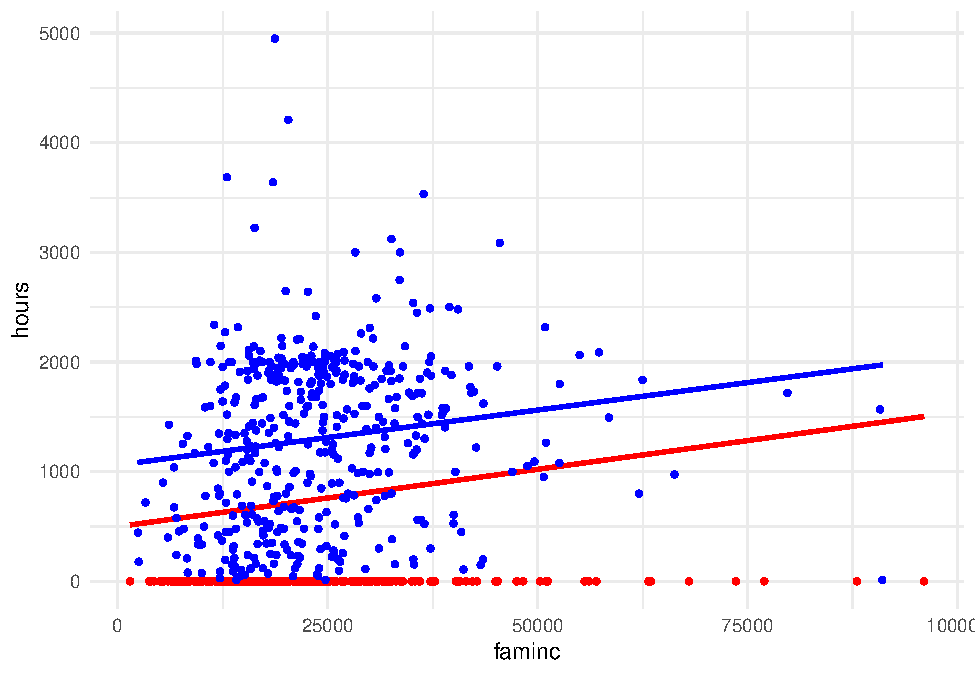
\includegraphics{rEkonometri_files/figure-latex/unnamed-chunk-194-1.pdf}

Sansürlenmiş örneklemleri aşmak için tobit modelini kullanacağız.

Kısa bir bilgi: Tobin (tobit regresyon modeli geliştiricisi), ilk kez dayanıklı tüketim malları üzerine hane halkı harcamalarını analiz ederken, kimi ailelerin dayanıklı tüketim malı harcaması gibi bir harcama kaleminin olmaması sebebiyle bağımlı değişkeni negatif çıkan bir regresyon türü ile karşılaşmıştır. Tobin bu çalışmasında, harcamanın hiçbir zaman negatif olmayacağı gerçeğinden hareketle hane halkı geliri, belli bir düzeyi geçene kadar bu değişkene sıfır değeri atamıştır. O yıllarda tanımladığı bu model sansürlü regresyon modeline klasik bir örnektir.

\begin{Shaded}
\begin{Highlighting}[]
\NormalTok{tobitmodel <-}\StringTok{ }\KeywordTok{vglm}\NormalTok{(hours }\OperatorTok{~}\NormalTok{., tobit, }\DataTypeTok{data =}\NormalTok{ df1 }\OperatorTok\StringTok{ }\NormalTok{dplyr}\OperatorTok{::}\KeywordTok{select}\NormalTok{(}\OperatorTok{-}\NormalTok{lfp))}
\KeywordTok{summary}\NormalTok{(tobitmodel)}
\end{Highlighting}
\end{Shaded}

\begin{verbatim}
## 
## Call:
## vglm(formula = hours ~ ., family = tobit, data = df1 %>% dplyr::select(-lfp))
## 
## Pearson residuals:
##                  Min      1Q  Median     3Q    Max
## mu          -10.1977 -0.7731 -0.1636 0.7504  4.053
## loglink(sd)  -0.9917 -0.5884 -0.2539 0.1925 13.300
## 
## Coefficients: 
##                 Estimate Std. Error z value Pr(>|z|)    
## (Intercept):1  1.126e+03  3.796e+02   2.967 0.003010 ** 
## (Intercept):2  6.964e+00  3.557e-02 195.793  < 2e-16 ***
## age           -5.411e+01  6.549e+00  -8.262  < 2e-16 ***
## educ           3.865e+01  2.063e+01   1.873 0.061019 .  
## exper          1.298e+02  1.597e+01   8.131 4.24e-16 ***
## expersq       -1.845e+00  5.012e-01  -3.681 0.000233 ***
## faminc         4.077e-02  5.275e-03   7.729 1.09e-14 ***
## kidsl6        -7.824e+02  1.024e+02  -7.637 2.22e-14 ***
## hwage         -1.055e+02  1.571e+01  -6.718 1.84e-11 ***
## ---
## Signif. codes:  0 '***' 0.001 '**' 0.01 '*' 0.05 '.' 0.1 ' ' 1
## 
## Names of linear predictors: mu, loglink(sd)
## 
## Log-likelihood: -3789.858 on 1497 degrees of freedom
## 
## Number of Fisher scoring iterations: 6 
## 
## No Hauck-Donner effect found in any of the estimates
\end{verbatim}

Bir bağımsız değişkenin tobit parametresinin bu bağımsız değişkenin gözlenen bağımlı değişken ortalama değeri üzerindeki marjinal etkisini verdiği şeklinde yorumlayamayız. Yani, Sıradan En Küçük Kareler yorumu geçerli değildir. Nedeni ise tobit türündeki sansürlenmiş regresyon modellerinde bağımsız değişken değerindeki 1 birimlik değişimin iki tane olan etkisindendir. Bu iki etkiden birincisi, gözlenen bağımlı değişkenin ortalama değere; ikincisi, gizli değişkenin gerçekte gözlenme olasılığına etkisidir. Örnek olarak age değişkenini alalım. Parametresi 54'tür. Diğer değişkenler sabit tutulduğunda, yaştaki 1 yıllık artışın yıllık çalışma saati olan hours'a doğrudan etkisi 54 saatlik düşüştür. Bunun yanında evli bir kadının işgücüne katılma olasılığının da azalması anlamındadır. Bu nedenle bizim 54'ü bunun gerçekleşme olasılığı ile çarpmamız gerekiyor.

Tobit modelde hata teriminin sıfır ortalamalı ve sabit varyanslı normal dağılım izlediği varsayılır.

Şimdi başa dönelim. 753 kadın değil de 428'i üzerinden Sıradan En Küçük Kareler yöntemini çalıştırmak istemediğimizi söylemiştik. Dolayısıyla örneklem kırpılmış olduğundan kırpılmış normal dağılımı kullanmamız gerekir. Bu modeli kurmak için de en çok olabilirlik gibi doğrusal olmayan bir tahmin yöntemi kullanmalıyız.

\begin{Shaded}
\begin{Highlighting}[]
\NormalTok{mlmodel <-}\StringTok{ }\KeywordTok{truncreg}\NormalTok{(hours }\OperatorTok{~}\NormalTok{., }\DataTypeTok{data =}\NormalTok{ df1 }\OperatorTok\StringTok{ }\KeywordTok{filter}\NormalTok{(lfp }\OperatorTok{==}\StringTok{ }\DecValTok{1}\NormalTok{) }\OperatorTok\StringTok{ }\NormalTok{dplyr}\OperatorTok{::}\KeywordTok{select}\NormalTok{(}\OperatorTok{-}\NormalTok{lfp), }\DataTypeTok{scaled =} \OtherTok{TRUE}\NormalTok{)}
\KeywordTok{summary}\NormalTok{(mlmodel)}
\end{Highlighting}
\end{Shaded}

\begin{verbatim}
## 
## Call:
## truncreg(formula = hours ~ ., data = df1 %>% filter(lfp == 1) %>% 
##     dplyr::select(-lfp), scaled = TRUE)
## 
## BFGS maximization method
## 0 iterations, 0h:0m:0s 
## g'(-H)^-1g = 0.000217 
##  
## 
## 
## Coefficients :
##                Estimate  Std. Error t-value  Pr(>|t|)    
## (Intercept)  1.8637e+03  4.0429e+02  4.6098 4.030e-06 ***
## age         -2.2892e+01  7.3239e+00 -3.1257 0.0017739 ** 
## educ        -5.0796e+01  2.1568e+01 -2.3552 0.0185143 *  
## exper        7.3749e+01  1.9167e+01  3.8477 0.0001193 ***
## expersq     -9.5576e-01  5.5560e-01 -1.7202 0.0853915 .  
## faminc       3.6207e-02  5.3203e-03  6.8054 1.008e-11 ***
## kidsl6      -3.9196e+02  1.3940e+02 -2.8118 0.0049272 ** 
## hwage       -9.3575e+01  1.8413e+01 -5.0820 3.736e-07 ***
## sigma        7.9519e+02  3.8983e+01 20.3985 < 2.2e-16 ***
## ---
## Signif. codes:  0 '***' 0.001 '**' 0.01 '*' 0.05 '.' 0.1 ' ' 1
## 
## Log-Likelihood: -3370 on 9 Df
\end{verbatim}

428 kadın üzerinden modeli kurmuş olduk. En başta Sıradan En Küçük Kareler yöntemi ile de model kurmuştuk. Parametre büyüklükleri ve istatistiksel anlamlılıklarda farklılıklar göreceğiz. Örneğin, sansürlenmiş modelde educ parametresi pozitifti. Kırpılmış regresyonda ise educ parametresi negatif çıktı.

O halde sansürlenmiş ve kırpılmış regresyon modellerinden hangisi daha uygundur? \emph{Tobit model (753 gözlem) kırpılmış regresyon modelinden (428 gözlem) daha fazla bilgi kullandığından, tobit modelden elde edilen tahminlerin daha etkin olacağı beklenir} der Gujarati.

Bir uygulama daha yapacağız. Fakat uygulamaya geçmeden önce iki kavramı biraz daha açalım: Sansürlenmiş, kırpılmış.

Kırpılmış regresyon modeli sansürlenmiş regresyon modelinden önemli bir noktada ayrılır. Veri sansürleme durumunda rassal çekilen her bir birim için hep bağımsız değişkenleri gözlerken veri yalnızca bir eşiğin altında veya üstünde sansürlenmediği zaman Y'nin sonucunu gözleriz. Veri budama ile dikkatimizi örnekleme öncesi anakütlenin bir alt setine sınırlıyoruz; böylece bilgi gözlemediğimiz anakütlenin bir parçası mevcuttur. Bir kırpılmış regresyon modeli örneklemimizdeki anakütlenin bir alt setini dışladığımızda ortaya çıkar. Bağımlı değişkenin değişim aralığının herhangi bir şekilde sınırlandırıldığı regresyon modellerinde eğer belirli bir aralığın dışındaki gözlemler tamamen kaybedilmekte ise kırpılmış model, en azından bağımsız değişkenler gözlenebiliyorsa sansürlü model söz konusu olmaktadır.

İlk evliliklerindeki 601 kadın ve erkeğe ait bir örneklemde evlilik dışı ilişki hakkında sorular sorulmuş ve tepkileri ölçülmüş.

\begin{Shaded}
\begin{Highlighting}[]
\NormalTok{df2 }\OperatorTok\StringTok{ }
\StringTok{  }\NormalTok{dplyr}\OperatorTok{::}\KeywordTok{select}\NormalTok{(naffairs, age, male, educ, kids, ratemarr, relig, yrsmarr)}
\end{Highlighting}
\end{Shaded}

\begin{itemize}
\item
  \textbf{naffairs:} Bağımlı değişkendir. Geçmiş yıldaki evlilik dışı ilişki sayısı
\item
  \textbf{age:} Yaş
\item
  \textbf{male:} Erkek ise 1
\item
  \textbf{educ:} Eğitim yılı
\item
  \textbf{kids:} Çocuk varsa 1
\item
  \textbf{ratemarr:} Evlilik değerlendirmesi (çok mutsuz 1, .., çok mutlu 5)
\item
  \textbf{relig:} Dindarlık seviyesi (dindar değil 1, .., çok dindar 5)
\item
  \textbf{yrsmarr:} Evlilik yılı
\end{itemize}

Referans olması açısından Sıradan En Küçük Kareler yöntemi ile bir model kuralım.

\begin{Shaded}
\begin{Highlighting}[]
\NormalTok{modelref <-}\StringTok{ }\KeywordTok{lm}\NormalTok{(naffairs }\OperatorTok{~}\NormalTok{., }\DataTypeTok{data =}\NormalTok{ df2)}
\KeywordTok{summary}\NormalTok{(modelref)}
\end{Highlighting}
\end{Shaded}

\begin{verbatim}
## 
## Call:
## lm(formula = naffairs ~ ., data = df2)
## 
## Residuals:
##     Min      1Q  Median      3Q     Max 
## -4.8606 -1.7508 -0.7755  0.1734 12.6532 
## 
## Coefficients:
##             Estimate Std. Error t value Pr(>|t|)    
## (Intercept)  5.75759    1.13373   5.078 5.10e-07 ***
## age         -0.04910    0.02257  -2.176    0.030 *  
## male         0.16970    0.28417   0.597    0.551    
## educ         0.01799    0.05825   0.309    0.758    
## kids        -0.21898    0.34428  -0.636    0.525    
## ratemarr    -0.71671    0.11998  -5.974 4.00e-09 ***
## relig       -0.48251    0.11169  -4.320 1.83e-05 ***
## yrsmarr      0.17125    0.04121   4.155 3.73e-05 ***
## ---
## Signif. codes:  0 '***' 0.001 '**' 0.01 '*' 0.05 '.' 0.1 ' ' 1
## 
## Residual standard error: 3.096 on 593 degrees of freedom
## Multiple R-squared:  0.1297, Adjusted R-squared:  0.1194 
## F-statistic: 12.62 on 7 and 593 DF,  p-value: 3.841e-15
\end{verbatim}

age, ratemarr, relig ve yrsmarr değişkenlerinin işaretleri beklentilere paraleldir. Ayrıca istatistiksel olarak da anlamlı çıkmışlardır. Fakat bu veriler sansürlenmiştir. Bu nedenle tahmin edilen parametreler muhtemelen yanlıdır ve tutarlı değildir. Sansürlemeyi hesaba katmak için tobit modelini tahmin edelim. İki modeli de yan yana koyduğumuz zaman tahmin edilen parametrelerinde ve istatistiksel anlamlılıklarında farklılıklar olduğunu göreceğiz.

\begin{Shaded}
\begin{Highlighting}[]
\NormalTok{tobitmodel <-}\StringTok{ }\KeywordTok{vglm}\NormalTok{(naffairs }\OperatorTok{~}\NormalTok{., tobit, }\DataTypeTok{data =}\NormalTok{ df2)}
\KeywordTok{summary}\NormalTok{(tobitmodel)}
\end{Highlighting}
\end{Shaded}

\begin{verbatim}
## 
## Call:
## vglm(formula = naffairs ~ ., family = tobit, data = df2)
## 
## Pearson residuals:
##                 Min      1Q  Median      3Q    Max
## mu          -11.720 -0.5219 -0.3157 -0.1020  5.142
## loglink(sd)  -1.009 -0.2831 -0.2551 -0.1405 11.546
## 
## Coefficients: 
##               Estimate Std. Error z value Pr(>|z|)    
## (Intercept):1  7.36529    3.93373   1.872 0.061159 .  
## (Intercept):2  2.11272    0.06573  32.142  < 2e-16 ***
## age           -0.19042    0.08101  -2.351 0.018743 *  
## male           1.18311    1.00894   1.173 0.240943    
## educ           0.09239    0.20369   0.454 0.650135    
## kids           0.89845    1.27896   0.702 0.482375    
## ratemarr      -2.28996    0.41493  -5.519 3.41e-08 ***
## relig         -1.70985    0.40944  -4.176 2.97e-05 ***
## yrsmarr        0.53799    0.14696   3.661 0.000251 ***
## ---
## Signif. codes:  0 '***' 0.001 '**' 0.01 '*' 0.05 '.' 0.1 ' ' 1
## 
## Names of linear predictors: mu, loglink(sd)
## 
## Log-likelihood: -704.9511 on 1193 degrees of freedom
## 
## Number of Fisher scoring iterations: 7 
## 
## No Hauck-Donner effect found in any of the estimates
\end{verbatim}

Uygulamada sansürlenmiş regresyon modeller budanmış regresyon modellere tercih edilebilir. Çünkü ilkinde örneklemdeki bütün gözlemleri; ikincisinde sadece budanmışları dahil ederiz.

\hypertarget{sayma-verilerini-modelleme}{%
\chapter{Sayma Verilerini Modelleme}\label{sayma-verilerini-modelleme}}

\hypertarget{poisson-regresyon}{%
\section{Poisson Regresyon}\label{poisson-regresyon}}

\begin{itemize}
\item
  Bir ailenin bir yılda çıktığı tatil sayısı,
\item
  Bir firmanın bir yılda aldığı patent sayısı,
\item
  Bir yılda doktora ya da dişçiye gitme sayısı,
\item
  Bir haftada manava gitme sayısı,
\item
  Bir yılda alınan park cezası ya da hız cezası sayısı,
\item
  Belirli bir zaman diliminde hastanede kalınan gün sayısı,
\item
  Beş dakikalık bir zaman diliminde paralı yol gişesinden geçen araç sayısı,
\item
  Bir yılda sinema, tiyatro ya da operaya gitme sayısı \ldots{}
\end{itemize}

Bunun gibi örneklerde bağımlı değişken sayma türündendir. Söz konusu değişkenlerin değeri kesikli ve sonlu sayıdadır. Aynı zamanda aşağıdaki gibi nadir olaylara ilişkin örnekleri de verebiliriz:

\begin{itemize}
\item
  Bir haftalık sürede yıldırım çarpmasına uğramak,
\item
  iki hafta içinde birden çok loto kazanmak,
\item
  Dört hafta içinde iki ya da daha çok kalp krizi geçirmek,
\item
  Bir gün içerisinde en az bir trafik kazası geçirmek \ldots{}
\end{itemize}

Sayma verisine özellikle uyan olasılık dağılımı poisson olasılık dağılımıdır.

Poisson dağılımın olasılık yoğunluk fonksiyonu:

\(f(y_i) = \frac{(\mu^ye^{-\mu})}{y!}\)

y = 0, 1, 2, \ldots{}

f(y), y değişkeninin negatif olmayan tamsayılı değerler alma olasılığıdır.

y! = y * (y-1) * (y-2) * 2 * 1

Poisson dağılımda varyans ortalama ile aynı değere sahiptir (eşit yayılım). Yani;

e(y) = \(\mu\)

var(y) = \(\mu\)

Poisson regresyon modeli şöyle yazılabilir:

\(y_i = e(y_i) + \epsilon_i = \mu_i + \epsilon_i\)

y'ler birbirinden bağımsız dağılmış ve ortalaması \(\mu_i\) olan poisson rassal değişkenlerdir. Şöyle gösterebiliriz:

\(\mu_i = e(y_i) = exp(\beta_1 + \beta_2x_{2i} + ... + \beta_kx_{ki})\) ; exp: doğal logaritma tabanı e'nin () içindeki ifade kadar üssüdür.

Burada x'ler ortalama değeri etkileyebilecek bazı değişkenlerdir. Örneğin, sayma değişkenimiz bir kimsenin Babylon'daki etkinliklere bir yılda katılma sayısı olsun. Bu sayı gelire, ücrete, konum olarak uzaklığa ve otopark parasına bağlı olabilir.

Tahmin amacıyla modeli şöyle yazalım:

\(f(y_i) = \frac{(\mu^ye^{-\mu})}{y!} + \epsilon_i\)

\begin{Shaded}
\begin{Highlighting}[]
\KeywordTok{library}\NormalTok{(readxl);}\KeywordTok{library}\NormalTok{(tidyverse);}\KeywordTok{library}\NormalTok{(magrittr);}\KeywordTok{library}\NormalTok{(moments);}\KeywordTok{library}\NormalTok{(MASS)}

\KeywordTok{setwd}\NormalTok{(}\StringTok{"C:/Users/datanerd/Desktop/Github/rEkonometri/data"}\NormalTok{)}
\NormalTok{df <-}\StringTok{ }\KeywordTok{read_excel}\NormalTok{(}\StringTok{"Table12_1.xls"}\NormalTok{)}
\end{Highlighting}
\end{Shaded}

1990 yılı için 181 uluslararası imalatçı firmadan oluşan veri seti patentler ve Ar-Ge harcamaları olacak.

Amacımız Ar-Ge, endüstri kategorisi ve iki ülkenin, 181 firmanın almış olduğu ortalama patent sayısına etkisini belirlemektir.

Öncelikle patentlerin, Ar-Ge logaritması (lr90 sütunu), beş endüstri (aerosp, chemist, computer, machines, vehicles) kuklası ve iki ülke (Japan, US) kuklasına göre regresyonunu alarak doğrusal bir regresyon modeli kurmak olacak. Bunu karşılaştırma amacıyla yapacağız.

\begin{Shaded}
\begin{Highlighting}[]
\KeywordTok{str}\NormalTok{(df)}
\end{Highlighting}
\end{Shaded}

\begin{verbatim}
## tibble [181 x 11] (S3: tbl_df/tbl/data.frame)
##  $ p91     : num [1:181] 55 67 55 83 0 4 7 0 0 96 ...
##  $ p90     : num [1:181] 80 46 42 102 1 11 55 0 1 67 ...
##  $ lr91    : num [1:181] 6.29 5.15 4.17 6.13 4.87 ...
##  $ lr90    : num [1:181] 6.16 5.14 4.1 6.15 4.82 ...
##  $ aerosp  : num [1:181] 0 0 0 0 0 0 1 0 0 0 ...
##  $ chemist : num [1:181] 0 0 1 1 0 0 0 0 0 1 ...
##  $ computer: num [1:181] 0 0 0 0 0 0 0 0 1 0 ...
##  $ machines: num [1:181] 0 0 0 0 0 0 0 0 0 0 ...
##  $ vehicles: num [1:181] 0 0 0 0 0 0 0 0 0 0 ...
##  $ japan   : num [1:181] 0 0 0 0 0 0 0 0 0 0 ...
##  $ us      : num [1:181] 1 1 1 0 0 0 1 1 1 1 ...
\end{verbatim}

\begin{Shaded}
\begin{Highlighting}[]
\NormalTok{lmodel <-}\StringTok{ }\KeywordTok{lm}\NormalTok{(}\DataTypeTok{formula =}\NormalTok{ p90 }\OperatorTok{~}\StringTok{ }\NormalTok{lr90 }\OperatorTok{+}\StringTok{ }\NormalTok{aerosp }\OperatorTok{+}\StringTok{ }\NormalTok{chemist }\OperatorTok{+}\StringTok{ }\NormalTok{computer }\OperatorTok{+}\StringTok{ }\NormalTok{machines }\OperatorTok{+}\StringTok{ }\NormalTok{vehicles }\OperatorTok{+}\StringTok{ }\NormalTok{japan }\OperatorTok{+}\StringTok{ }\NormalTok{us, }\DataTypeTok{data =}\NormalTok{ df)}
\KeywordTok{summary}\NormalTok{(lmodel)}
\end{Highlighting}
\end{Shaded}

\begin{verbatim}
## 
## Call:
## lm(formula = p90 ~ lr90 + aerosp + chemist + computer + machines + 
##     vehicles + japan + us, data = df)
## 
## Residuals:
##     Min      1Q  Median      3Q     Max 
## -339.29  -52.05   -4.73   37.48  585.04 
## 
## Coefficients:
##             Estimate Std. Error t value Pr(>|t|)    
## (Intercept) -250.839     55.435  -4.525 1.12e-05 ***
## lr90          73.172      7.971   9.180  < 2e-16 ***
## aerosp       -44.162     35.645  -1.239  0.21706    
## chemist       47.081     26.542   1.774  0.07786 .  
## computer      33.856     27.769   1.219  0.22444    
## machines      34.379     27.813   1.236  0.21811    
## vehicles    -191.790     36.704  -5.225 4.98e-07 ***
## japan         26.239     40.920   0.641  0.52223    
## us           -76.854     28.649  -2.683  0.00802 ** 
## ---
## Signif. codes:  0 '***' 0.001 '**' 0.01 '*' 0.05 '.' 0.1 ' ' 1
## 
## Residual standard error: 114.5 on 172 degrees of freedom
## Multiple R-squared:  0.4729, Adjusted R-squared:  0.4484 
## F-statistic: 19.29 on 8 and 172 DF,  p-value: < 2.2e-16
\end{verbatim}

Ar-Ge harcamaları (lr90) ile patent sayısı (p90) arasında istatistiksel olarak oldukça anlamlı pozitif bir ilişki bulunmaktadır. Ar-Ge değişkeni logaritmik; patent değişkeni ise doğrusal yapıdadır.

Diğer değişkenler sabit tutulduğunda;

Ar-Ge harcamalarındaki \%1'lik artış ortalama patent sayısını 0.73 kadar artırır.

Endüstrilerde ise chemist ve vehicles anlamlıdır. Parametrelerine baktığımızda chemist'te verilen ortalama patent miktarı 47 patent daha fazladır; vehicles'da verilen ortalama patent miktarı 192 patent daha düşüktür.

Ülkelere göre baktığımızda sadece us anlamlıdır. Burada, us firmalarının baz gruba göre ortalamada 77 daha az patent almış olduğunu söyleyebiliriz.

Bu modeli karşılaştırma amaçlı kurduğumuzu söylemiştik. ve bu modelin uygun olmadığını göstermiş olduk. Çünkü bazı firmalar büyük sayıda patentler almış olsalar da firma başına bir yılda alınan patent sayısı genellikle düşüktür. Bunu görselleştirelim.

\begin{Shaded}
\begin{Highlighting}[]
\NormalTok{df }\OperatorTok\StringTok{ }
\StringTok{  }\KeywordTok{ggplot}\NormalTok{(}\KeywordTok{aes}\NormalTok{(}\DataTypeTok{x =}\NormalTok{ p90)) }\OperatorTok{+}
\StringTok{  }\KeywordTok{geom_histogram}\NormalTok{() }\OperatorTok{+}
\StringTok{  }\KeywordTok{geom_vline}\NormalTok{(}\DataTypeTok{xintercept =} \DecValTok{200}\NormalTok{, }\DataTypeTok{linetype=}\StringTok{"dashed"}\NormalTok{) }\OperatorTok{+}
\StringTok{  }\KeywordTok{theme_minimal}\NormalTok{()}
\end{Highlighting}
\end{Shaded}

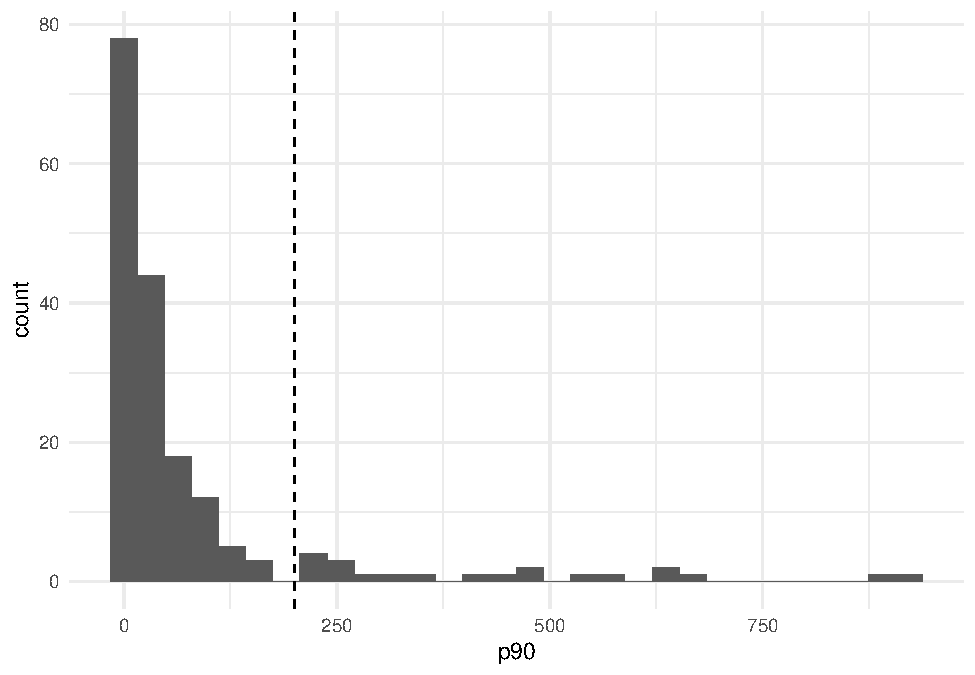
\includegraphics{rEkonometri_files/figure-latex/unnamed-chunk-203-1.pdf}

Firmaların büyük bir çoğunluğunun 200'den daha az patent aldığını görselden net bir şekilde görebiliyoruz. Bu durumu tablo şeklinde de gösterebiliriz.

\begin{Shaded}
\begin{Highlighting}[]
\NormalTok{df }\OperatorTok\StringTok{ }
\StringTok{  }\KeywordTok{mutate}\NormalTok{(}\DataTypeTok{patentler =} \KeywordTok{ifelse}\NormalTok{(p90 }\OperatorTok\StringTok{ }\DecValTok{0}\OperatorTok{:}\DecValTok{199}\NormalTok{, }\StringTok{"[0-200)"}\NormalTok{,}
                            \KeywordTok{ifelse}\NormalTok{(p90 }\OperatorTok\StringTok{ }\DecValTok{200}\OperatorTok{:}\DecValTok{399}\NormalTok{, }\StringTok{"[200-400)"}\NormalTok{,}
                                   \KeywordTok{ifelse}\NormalTok{(p90 }\OperatorTok\StringTok{ }\DecValTok{400}\OperatorTok{:}\DecValTok{599}\NormalTok{, }\StringTok{"[400-600)"}\NormalTok{,}
                                          \KeywordTok{ifelse}\NormalTok{(p90 }\OperatorTok\StringTok{ }\DecValTok{600}\OperatorTok{:}\DecValTok{799}\NormalTok{, }\StringTok{"[600-800)"}\NormalTok{,}
                                                 \KeywordTok{ifelse}\NormalTok{(p90 }\OperatorTok\StringTok{ }\DecValTok{800}\OperatorTok{:}\DecValTok{999}\NormalTok{, }\StringTok{"[800-1000)"}\NormalTok{, }\StringTok{""}\NormalTok{)))))) }\OperatorTok\StringTok{ }
\StringTok{  }\KeywordTok{group_by}\NormalTok{(patentler) }\OperatorTok\StringTok{ }
\StringTok{  }\KeywordTok{summarise}\NormalTok{(}\StringTok{"sayı"}\NormalTok{ =}\StringTok{ }\KeywordTok{n}\NormalTok{()) }\OperatorTok\StringTok{ }
\StringTok{  }\KeywordTok{mutate}\NormalTok{(}\StringTok{"yüzde" = `sayı` / sum(`sayı`) * 100) %>% }
\StringTok{  mutate("}\NormalTok{kümülatif sayı}\StringTok{" = cumsum(`sayı`),}
\StringTok{         "}\NormalTok{kümülatif yüzde}\StringTok{" = cumsum(`yüzde`))}
\end{Highlighting}
\end{Shaded}

\begin{verbatim}
## # A tibble: 5 x 5
##   patentler   sayı yüzde `kümülatif sayı` `kümülatif yüzde`
##   <chr>      <int> <dbl>            <int>             <dbl>
## 1 [0-200)      160 88.4               160              88.4
## 2 [200-400)     10  5.52              170              93.9
## 3 [400-600)      6  3.31              176              97.2
## 4 [600-800)      3  1.66              179              98.9
## 5 [800-1000)     2  1.10              181             100
\end{verbatim}

Patent sayıları özellikle görselden görebileceğimiz gibi çarpık dağılmıştır. Çarpıklık (skewness) değeri:

\begin{Shaded}
\begin{Highlighting}[]
\KeywordTok{skewness}\NormalTok{(df}\OperatorTok{$}\NormalTok{p90)}
\end{Highlighting}
\end{Shaded}

\begin{verbatim}
## [1] 3.264074
\end{verbatim}

Basıklık (kurtosis) değeri ise:

\begin{Shaded}
\begin{Highlighting}[]
\KeywordTok{kurtosis}\NormalTok{(df}\OperatorTok{$}\NormalTok{p90)}
\end{Highlighting}
\end{Shaded}

\begin{verbatim}
## [1] 14.44027
\end{verbatim}

Normal dağılımlı bir değişken için skewness 0, kurtosis değeri 3'tür. Jarque-Bera istatistiği:

\begin{Shaded}
\begin{Highlighting}[]
\KeywordTok{jarque.test}\NormalTok{(df}\OperatorTok{$}\NormalTok{p90)}
\end{Highlighting}
\end{Shaded}

\begin{verbatim}
## 
##  Jarque-Bera Normality Test
## 
## data:  df$p90
## JB = 1308.5, p-value < 2.2e-16
## alternative hypothesis: greater
\end{verbatim}

Mevcut örnekte 1308 olarak tahmin edilen J-B değeri o kadar büyüktür ki, en az bu değeri elde etme olasılığı neredeyse sıfırdır.

Kısaca, sayma verilerini modellemek için normal olasılık dağılımını kullanamayacak; poisson olasılık dağılımınını kullanacağız.

\begin{Shaded}
\begin{Highlighting}[]
\NormalTok{pmodel <-}\StringTok{ }\KeywordTok{glm}\NormalTok{(}\DataTypeTok{formula =}\NormalTok{ p90 }\OperatorTok{~}\StringTok{ }\NormalTok{lr90 }\OperatorTok{+}\StringTok{ }\NormalTok{aerosp }\OperatorTok{+}\StringTok{ }\NormalTok{chemist }\OperatorTok{+}\StringTok{ }\NormalTok{computer }\OperatorTok{+}\StringTok{ }\NormalTok{machines }\OperatorTok{+}\StringTok{ }\NormalTok{vehicles }\OperatorTok{+}\StringTok{ }\NormalTok{japan }\OperatorTok{+}\StringTok{ }\NormalTok{us, }\DataTypeTok{family =} \StringTok{"poisson"}\NormalTok{, }\DataTypeTok{data =}\NormalTok{ df)}
\KeywordTok{summary}\NormalTok{(pmodel)}
\end{Highlighting}
\end{Shaded}

\begin{verbatim}
## 
## Call:
## glm(formula = p90 ~ lr90 + aerosp + chemist + computer + machines + 
##     vehicles + japan + us, family = "poisson", data = df)
## 
## Deviance Residuals: 
##     Min       1Q   Median       3Q      Max  
## -27.163   -5.210   -1.752    2.942   28.359  
## 
## Coefficients:
##              Estimate Std. Error z value Pr(>|z|)    
## (Intercept) -0.745849   0.062136 -12.003   <2e-16 ***
## lr90         0.865149   0.008068 107.234   <2e-16 ***
## aerosp      -0.796538   0.067953 -11.722   <2e-16 ***
## chemist      0.774751   0.023126  33.501   <2e-16 ***
## computer     0.468894   0.023939  19.587   <2e-16 ***
## machines     0.646383   0.038033  16.995   <2e-16 ***
## vehicles    -1.505641   0.039176 -38.433   <2e-16 ***
## japan       -0.003893   0.026866  -0.145    0.885    
## us          -0.418938   0.023094 -18.141   <2e-16 ***
## ---
## Signif. codes:  0 '***' 0.001 '**' 0.01 '*' 0.05 '.' 0.1 ' ' 1
## 
## (Dispersion parameter for poisson family taken to be 1)
## 
##     Null deviance: 30808  on 180  degrees of freedom
## Residual deviance:  9326  on 172  degrees of freedom
## AIC: 10181
## 
## Number of Fisher Scoring iterations: 5
\end{verbatim}

Sadece japan parametresi istatistiksel olarak anlamlı değildir.

lr90 0.8651 çıktı. Ar-Ge harcamaları \%1 arttığında bir firmaya verilen ortalama patent sayısı \%0.86 artar ya da verilen patentlerin arge harcamalarına göre esnekliği 0.86'dır.

Endüstriler arasından machines'i seçelim. machines endüstrisindeki ortalama patent sayısı, karşılaştırma kategorisine göre \% aşağıdaki kadar daha yüksektir.

\begin{Shaded}
\begin{Highlighting}[]
\DecValTok{100} \OperatorTok{*}\StringTok{ }\NormalTok{(}\KeywordTok{exp}\NormalTok{(}\FloatTok{0.6464}\NormalTok{) }\OperatorTok{-}\StringTok{ }\DecValTok{1}\NormalTok{)}
\end{Highlighting}
\end{Shaded}

\begin{verbatim}
## [1] 90.86573
\end{verbatim}

Ülkeler arasından us'i seçelim. Baz grupla karşılaştırıldığında us kukla parametresi \% aşağıdaki kadar daha düşüktür.

\begin{Shaded}
\begin{Highlighting}[]
\DecValTok{100} \OperatorTok{*}\StringTok{ }\NormalTok{(}\KeywordTok{exp}\NormalTok{(}\OperatorTok{-}\FloatTok{0.4189}\NormalTok{) }\OperatorTok{-}\StringTok{ }\DecValTok{1}\NormalTok{)}
\end{Highlighting}
\end{Shaded}

\begin{verbatim}
## [1] -34.223
\end{verbatim}

Biz bir tek parametrelerin istatistiksel olarak anlamlı olup olmadığına bakıp yorum yaptık ama bu şekilde modeli kabul edip konuyu bitirmemiz söz konusu olamaz.

Parametre tahminlerinin yukarıdaki tabloda verilen standart hataları, ancak tahmin edilen modelde poisson dağılımı olduğu varsayımı doğruysa geçerlidir. Yazının başında şunu demiştik: Poisson dağılımda varyans ortalama ile aynı değere sahiptir (eşit yayılım). Bunu kontrol etmemiz gerekiyor.

Eğer aşırı yayılım varsa poisson regresyon modeli tahminleri tutarlı olmasına rağmen etkin değildir. Çünkü standart hatalar aşağı yönlü sapmalıdır. Eğer durum böyleyse, tahmin edilen z değerleri yükselmiş olur ve böylece parametre tahminlerinin istatistiksel anlamlılığını yüksek tahmin eder.

\begin{Shaded}
\begin{Highlighting}[]
\NormalTok{asiriyayilim <-}\StringTok{ }\KeywordTok{glm}\NormalTok{(}\DataTypeTok{formula =}\NormalTok{ p90 }\OperatorTok{~}\StringTok{ }\NormalTok{lr90 }\OperatorTok{+}\StringTok{ }\NormalTok{aerosp }\OperatorTok{+}\StringTok{ }\NormalTok{chemist }\OperatorTok{+}\StringTok{ }\NormalTok{computer }\OperatorTok{+}\StringTok{ }\NormalTok{machines }\OperatorTok{+}\StringTok{ }\NormalTok{vehicles }\OperatorTok{+}\StringTok{ }\NormalTok{japan }\OperatorTok{+}\StringTok{ }\NormalTok{us, }\DataTypeTok{family =} \StringTok{"quasipoisson"}\NormalTok{, }\DataTypeTok{data =}\NormalTok{ df) }
\KeywordTok{summary}\NormalTok{(asiriyayilim)}\OperatorTok{$}\NormalTok{dispersion}
\end{Highlighting}
\end{Shaded}

\begin{verbatim}
## [1] 61.9516
\end{verbatim}

\begin{Shaded}
\begin{Highlighting}[]
\KeywordTok{pchisq}\NormalTok{(}\KeywordTok{summary}\NormalTok{(asiriyayilim)}\OperatorTok{$}\NormalTok{dispersion }\OperatorTok{*}\StringTok{ }\NormalTok{pmodel}\OperatorTok{$}\NormalTok{df.residual, pmodel}\OperatorTok{$}\NormalTok{df.residual, }\DataTypeTok{lower =} \OtherTok{FALSE}\NormalTok{)}
\end{Highlighting}
\end{Shaded}

\begin{verbatim}
## [1] 0
\end{verbatim}

Bu sonuç aşırı yayılım olduğunu gösterir.

\hypertarget{negatif-binom-regresyon}{%
\section{Negatif Binom Regresyon}\label{negatif-binom-regresyon}}

Burada alternatif bir yol olan negatif binom regresyon modeline kaçılabilir. Bu model için varyans ortalamadan daima büyüktür. Negatif binom olasılık dağılımı için \(\sigma^2 = \mu + \frac{\mu^2}{r}\) ; \(\mu\) \textgreater{} 0, r \textgreater{} 0 (r: başarı sayısı) olduğu gösterilebilir. Bu eşitlik, negatif binom olasılık dağılımı için varyansın ortalamadan daima büyük olduğunu gösterir.

\begin{Shaded}
\begin{Highlighting}[]
\NormalTok{nbmodel <-}\StringTok{ }\KeywordTok{glm.nb}\NormalTok{(}\DataTypeTok{formula =}\NormalTok{ p90 }\OperatorTok{~}\StringTok{ }\NormalTok{lr90 }\OperatorTok{+}\StringTok{ }\NormalTok{aerosp }\OperatorTok{+}\StringTok{ }\NormalTok{chemist }\OperatorTok{+}\StringTok{ }\NormalTok{computer }\OperatorTok{+}\StringTok{ }\NormalTok{machines }\OperatorTok{+}\StringTok{ }\NormalTok{vehicles }\OperatorTok{+}\StringTok{ }\NormalTok{japan }\OperatorTok{+}\StringTok{ }\NormalTok{us, }\DataTypeTok{data =}\NormalTok{ df)}
\KeywordTok{summary}\NormalTok{(nbmodel)}
\end{Highlighting}
\end{Shaded}

\begin{verbatim}
## 
## Call:
## glm.nb(formula = p90 ~ lr90 + aerosp + chemist + computer + machines + 
##     vehicles + japan + us, data = df, init.theta = 0.777306951, 
##     link = log)
## 
## Deviance Residuals: 
##     Min       1Q   Median       3Q      Max  
## -2.8148  -1.0293  -0.2992   0.2858   2.5906  
## 
## Coefficients:
##              Estimate Std. Error z value Pr(>|z|)    
## (Intercept) -0.407240   0.558801  -0.729   0.4661    
## lr90         0.867174   0.080344  10.793  < 2e-16 ***
## aerosp      -0.874436   0.364764  -2.397   0.0165 *  
## chemist      0.666191   0.265790   2.506   0.0122 *  
## computer    -0.132057   0.279389  -0.473   0.6365    
## machines     0.008171   0.282563   0.029   0.9769    
## vehicles    -1.515083   0.366812  -4.130 3.62e-05 ***
## japan        0.121004   0.407195   0.297   0.7663    
## us          -0.691413   0.285743  -2.420   0.0155 *  
## ---
## Signif. codes:  0 '***' 0.001 '**' 0.01 '*' 0.05 '.' 0.1 ' ' 1
## 
## (Dispersion parameter for Negative Binomial(0.7773) family taken to be 1)
## 
##     Null deviance: 427.54  on 180  degrees of freedom
## Residual deviance: 214.61  on 172  degrees of freedom
## AIC: 1690.9
## 
## Number of Fisher Scoring iterations: 1
## 
## 
##               Theta:  0.7773 
##           Std. Err.:  0.0820 
## 
##  2 x log-likelihood:  -1670.9010
\end{verbatim}

\hypertarget{dinamik-ekonometri-modelleri}{%
\chapter{Dinamik Ekonometri Modelleri}\label{dinamik-ekonometri-modelleri}}

Zaman serisine ait verilerin kullanıldığı bir regresyon analizinde eğer model, X bağımsız değişkenlerin sadece şimdiki değerlerini değil; gecikmeli ya da geçmişteki değerlerini de içeriyorsa bu modele gecikmesi dağıtılmış model denir. Eğer model, bağımsız değişkenleri arasında bağımlı değişkenin bir ya da birden fazla gecikmeli değerini içeriyorsa buna da otoregresif model denir.

Gecikmesi dağıtılmış model:

\(Y_t = \alpha + \beta_0X_t + \beta_1X_{t-1} + \beta_2X_{t-2} + \epsilon_t\)

Otoregresif model:

\(Y_t = \alpha + \beta X_t + \gamma Y_{t-1} + \epsilon_t\)

Gecikmeler psikolojik, teknolojik ve kurumsal nedenlerden dolayı ortaya çıkabilir.

\hypertarget{otoregresif-daux11fux131tux131lmux131ux15f-gecikme-modelleri-ardl}{%
\section{Otoregresif Dağıtılmış Gecikme Modelleri (ARDL)}\label{otoregresif-daux11fux131tux131lmux131ux15f-gecikme-modelleri-ardl}}

Bu modelleri daha genel bir dinamik regresyon modelinde birleştirebiliriz.

\(Y_t = \theta_0 + \theta_1Y_{t-1} + \theta_2Y_{t-2} + ... + \theta_pY_{t-p} + \beta_0X_t + \beta1X_{t-1} + \beta_2X_{t-2} + ... + \beta_qX_{t-q} + \epsilon_t\)

Yukarıdaki modelde p otoregresif terim; q ise dağıtılmış gecikme terimidir.

ARDL(p,q) olarak yazarsak, gecikmeli Y'ler otoregresif kısmı; gecikmeli X'ler dağıtılmış kısmı oluşturur.

ARDL ile sadece gecikmeli Y'lerin dinamik etkilerini değil, aynı zamanda gecikmeli X'lerin de dinamik etkilerini yakalayabiliriz.

Yine ARDL ile eğer yeterli gecikmeleri model içinde bulundurursak hata terimindeki otokorelasyonu saf dışı edebiliriz.

Aşağıdaki uygulama ile ARDL(1,1) modelini inceleyelim.

\begin{Shaded}
\begin{Highlighting}[]
\KeywordTok{library}\NormalTok{(readxl);}\KeywordTok{library}\NormalTok{(tidyverse);}\KeywordTok{library}\NormalTok{(magrittr);}\KeywordTok{library}\NormalTok{(ARDL);}\KeywordTok{library}\NormalTok{(lmtest);}\KeywordTok{library}\NormalTok{(sandwich)}

\KeywordTok{setwd}\NormalTok{(}\StringTok{"C:/Users/datanerd/Desktop/Github/rEkonometri/data"}\NormalTok{)}
\NormalTok{df <-}\StringTok{ }\KeywordTok{read_excel}\NormalTok{(}\StringTok{"pce_dpi.xls"}\NormalTok{)}

\KeywordTok{str}\NormalTok{(df)}
\end{Highlighting}
\end{Shaded}

\begin{verbatim}
## tibble [50 x 3] (S3: tbl_df/tbl/data.frame)
##  $ obs: num [1:50] 1960 1961 1962 1963 1964 ...
##  $ pce: num [1:50] 9871 9911 10243 10512 10985 ...
##  $ dpi: num [1:50] 10865 11052 11413 11672 12342 ...
\end{verbatim}

Bağımlı değişken:

\begin{itemize}
\tightlist
\item
  \textbf{pce:} Kişisel tüketim harcaması
\end{itemize}

Bağımsız değişken(ler):

\begin{itemize}
\tightlist
\item
  \textbf{dpi:} Vergi sonrası gelir
\end{itemize}

\(Y_t = \theta_0 + \theta_1Y_{t-1} + \beta_0X_t + \beta_1X_{t-1} + \epsilon_t, \theta_1 < 1\)

Burada, Y = pce ve X = dpi'dır.

Model şunu der: Cari dönemdeki kişisel tüketim harcaması (\(Y_t\)) hem bir önceki dönem kişisel tüketim harcamasıyla (\(Y_{t-1}\)) hem de cari (\(X_t\)) ve bir dönem önceki vergi sonrası gelir (\(X_{t-1}\)) ile ilişkilidir.

Vergi sonrası gelirdeki 1 birimlik değişimin etki çarpanı (anlık etkisi) \(\beta_0\)'dır.

Vergi sonrası gelirdeki birim değişim korunduğunda, uzun dönem çarpanı \(\frac{\beta_0 + \beta_1}{1 - \theta_1}\) olur. Bu aynı zamanda, vergi sonrası gelirin birim artışı korunduğunda kişisel tüketim harcamasındaki uzun dönemli sürekli artıştır.

ARDL(1,1) ile ilgili varsayımları atlamamamız gerekiyor.

\begin{itemize}
\item
  Y ve X değişkenleri durağandır (Zaman serisinde göreceğiz).
\item
  Yukarıda da yazdığımız aşağıdaki eşitlikte bağımsız değişken değerleri verildiğinde \(\epsilon_t\) hata teriminin beklenen ortalama değeri sıfırdır.
\end{itemize}

\(Y_t = \theta_0 + \theta_1Y_{t-1} + \theta_2Y_{t-2} + ... + \theta_pY_{t-p} + \beta_0X_t + \beta1X_{t-1} + \beta_2X_{t-2} + ... + \beta_qX_{t-q} + \epsilon_t\)

\begin{itemize}
\item
  Bir önceki maddede yazdığımız eşitlikte yer alan \(\epsilon_t\) hata terimi otokorelasyonlu değilse, bu durumda yazdığımız modelin ya da uygulamadaki modelin Sıradan En Küçük Kareler ile tahmin edilen parametreleri tutarlı olacaktır. Eğer \(\epsilon_t\) hata terimi otokorelasyonlu ise bu modellerdeki Y terimi de hata terimi ile korelasyonlu olacaktır. Bu durumda da Sıradan En Küçük Kareler tahmincileri tutarlı olmayacaktır.
\item
  X değişkenlerinin dışsal (en azından zayıf dışsal) olduğu varsayılır. Yani, hata terimi ile korelasyonlu değildirler.
\end{itemize}

\begin{Shaded}
\begin{Highlighting}[]
\NormalTok{model <-}\StringTok{ }\KeywordTok{ardl}\NormalTok{(}\DataTypeTok{formula =}\NormalTok{ pce }\OperatorTok{~}\StringTok{ }\NormalTok{dpi, }\DataTypeTok{data =}\NormalTok{ df, }\DataTypeTok{order =} \KeywordTok{c}\NormalTok{(}\DecValTok{1}\NormalTok{,}\DecValTok{1}\NormalTok{))}
\KeywordTok{summary}\NormalTok{(model)}
\end{Highlighting}
\end{Shaded}

\begin{verbatim}
## 
## Time series regression with "ts" data:
## Start = 2, End = 50
## 
## Call:
## dynlm::dynlm(formula = full_formula, data = data, start = start, 
##     end = end)
## 
## Residuals:
##     Min      1Q  Median      3Q     Max 
## -555.97 -112.46   10.89  126.53  557.68 
## 
## Coefficients:
##               Estimate Std. Error t value Pr(>|t|)    
## (Intercept) -281.20189  161.07123  -1.746   0.0877 .  
## L(pce, 1)      0.80536    0.08123   9.915 6.80e-13 ***
## dpi            0.82459    0.09798   8.416 8.61e-11 ***
## L(dpi, 1)     -0.63294    0.11886  -5.325 3.10e-06 ***
## ---
## Signif. codes:  0 '***' 0.001 '**' 0.01 '*' 0.05 '.' 0.1 ' ' 1
## 
## Residual standard error: 213.1 on 45 degrees of freedom
## Multiple R-squared:  0.9989, Adjusted R-squared:  0.9989 
## F-statistic: 1.396e+04 on 3 and 45 DF,  p-value: < 2.2e-16
\end{verbatim}

Vergi sonrası gelirdeki (dpi) 1 birimlik değişimin kişisel tüketim harcaması (pce) üzerindeki etki çarpanı (anlık etki) 0.82459'dur. Eğer bu 1 birimlik değişim korunuyorsa bu durumda uzun dönem çarpanı \(\frac{0.82459 + (-0.63294)}{1 - 0.80536} = 0.9846383\) olur. Beklentilere paralel olarak uzun dönem çarpan kısa dönem çarpandan büyüktür. Dolayısıyla vergi sonrası gelirdeki 1 \$'lık sürdürülebilir bir artış ortalama kişisel tüketim harcamasını 0.98 \$ kadar artıracaktır.

Otokorelasyon ihtimaline karşı hac yöntemi ile modeli tekrar kurabiliriz.

\begin{Shaded}
\begin{Highlighting}[]
\KeywordTok{coeftest}\NormalTok{(model, }\DataTypeTok{vcov =} \KeywordTok{NeweyWest}\NormalTok{(model))}
\end{Highlighting}
\end{Shaded}

\begin{verbatim}
## 
## t test of coefficients:
## 
##                Estimate  Std. Error t value  Pr(>|t|)    
## (Intercept) -281.201894  101.664501 -2.7660 0.0082027 ** 
## L(pce, 1)      0.805356    0.057375 14.0367 < 2.2e-16 ***
## dpi            0.824591    0.142609  5.7822 6.567e-07 ***
## L(dpi, 1)     -0.632942    0.152727 -4.1443 0.0001485 ***
## ---
## Signif. codes:  0 '***' 0.001 '**' 0.01 '*' 0.05 '.' 0.1 ' ' 1
\end{verbatim}

Hac yöntemi sadece standart hataları ve dolayısıyla t istatistiklerini ve p değerlerini değiştirir.

Eğer ilk kurduğumuz model ile karşılaştırırsak aralarında önemli bir fark olmadığını göreceğiz. Bu durum değişik otokorelasyon sınamalarına dayanan otokorelasyon kanıtlarına rağmen otokorelasyon sorununun çok ciddi görünmediğini ortaya koyar.

\hypertarget{dilim-kantil-regresyon}{%
\chapter{Dilim (Kantil) Regresyon}\label{dilim-kantil-regresyon}}

\emph{Bazen klasik modelin varsayım ihlallerine karşı, Sıradan En Küçük Kareler'den daha az duyarlı alternatifler olup olmadığına bakmak akıllıca olabilir} diyor Gujarati.

Biz bir olasılık dağılımının temel özelliklerini genellikle ortalama (beklenen değer), varyans, çarpıklık (simetri ölçüsü) ve basıklık (sivrilik derecesi) gibi momentler denilen özet nicelikler açısından ele alırız fakat dilim regresyon ile bunlara bakmak yerine bunları dilimler olarak adlandırılan dağılımın çeşitli segmentleri içinde inceleyebiliriz.

Dilim dediğimiz şey şunlardır: Dörttebirlikler, beştebirlikler, ondabirlikler, yüzdebirlikler/yüzdelikler. Gözlem sayısını belirtilen sayılarda eşit gruplara böleriz. Örneğin, bir arabanın fiyatının 75. yüzdelik dilimde olduğunu söylemek bu arabanın fiyatının diğer arabaların fiyatlarının \%75'ini aştığı anlamına gelir ya da aynı anlama gelecek şekilde \%75'inin x fiyatına veya x fiyatından daha az fiyata sahip olduğunu söyleyebiliriz. Bir olasılık dağılımının \%50 dilimi medyandır.

Y, kümülatif dağılım fonksiyonu ya da CDF'i F olan sürekli bir rassal değişken; p ise 0-1 arasında bir sayı olsun. Y'nin p.~dilimi \(Q_p\) değeridir. Yani;

Pr(Y ≤ \(Q_p\)) = F(\(Q_p\)) = p

Örneğin, \(Q_{0.75}\) = 5 ise Y ≤ 5 olma olasılığı 0.75'e eşittir. CDF'in altında ve \(Q_p\)'nin solunda kalan kısmın alanı p; \(Q_p\)'nin sağında kalan kısmın alanı ise 1-p'dir.

Şimdi dilim regresyon modeline bakabiliriz.

\begin{Shaded}
\begin{Highlighting}[]
\KeywordTok{library}\NormalTok{(readxl);}\KeywordTok{library}\NormalTok{(tidyverse);}\KeywordTok{library}\NormalTok{(magrittr);}\KeywordTok{library}\NormalTok{(quantreg)}

\KeywordTok{setwd}\NormalTok{(}\StringTok{"C:/Users/datanerd/Desktop/Github/rEkonometri/data"}\NormalTok{)}
\NormalTok{df <-}\StringTok{ }\KeywordTok{read_excel}\NormalTok{(}\StringTok{"Table1_1.xls"}\NormalTok{)}
\end{Highlighting}
\end{Shaded}

\begin{Shaded}
\begin{Highlighting}[]
\NormalTok{df }\OperatorTok\StringTok{ }
\StringTok{  }\NormalTok{dplyr}\OperatorTok{::}\KeywordTok{select}\NormalTok{(wage, female, nonwhite, union, education, exper)}
\end{Highlighting}
\end{Shaded}

Sıradan En Küçük Kareler çıktısını hatırlayalım:

\begin{Shaded}
\begin{Highlighting}[]
\NormalTok{model <-}\StringTok{ }\KeywordTok{lm}\NormalTok{(}\DataTypeTok{formula =}\NormalTok{ wage }\OperatorTok{~}\StringTok{ }\NormalTok{female }\OperatorTok{+}\StringTok{ }\NormalTok{nonwhite }\OperatorTok{+}\StringTok{ }\NormalTok{union }\OperatorTok{+}\StringTok{ }\NormalTok{education }\OperatorTok{+}\StringTok{ }\NormalTok{exper, }\DataTypeTok{data =}\NormalTok{ df)}
\KeywordTok{summary}\NormalTok{(model)}
\end{Highlighting}
\end{Shaded}

\begin{verbatim}
## 
## Call:
## lm(formula = wage ~ female + nonwhite + union + education + exper, 
##     data = df)
## 
## Residuals:
##     Min      1Q  Median      3Q     Max 
## -20.781  -3.760  -1.044   2.418  50.414 
## 
## Coefficients:
##             Estimate Std. Error t value Pr(>|t|)    
## (Intercept) -7.18334    1.01579  -7.072 2.51e-12 ***
## female      -3.07488    0.36462  -8.433  < 2e-16 ***
## nonwhite    -1.56531    0.50919  -3.074  0.00216 ** 
## union        1.09598    0.50608   2.166  0.03052 *  
## education    1.37030    0.06590  20.792  < 2e-16 ***
## exper        0.16661    0.01605  10.382  < 2e-16 ***
## ---
## Signif. codes:  0 '***' 0.001 '**' 0.01 '*' 0.05 '.' 0.1 ' ' 1
## 
## Residual standard error: 6.508 on 1283 degrees of freedom
## Multiple R-squared:  0.3233, Adjusted R-squared:  0.3207 
## F-statistic: 122.6 on 5 and 1283 DF,  p-value: < 2.2e-16
\end{verbatim}

wage değişkeninin dağılımına bakalım.

\begin{Shaded}
\begin{Highlighting}[]
\KeywordTok{ggplot}\NormalTok{(df, }\KeywordTok{aes}\NormalTok{(}\DataTypeTok{x =}\NormalTok{ wage)) }\OperatorTok{+}
\StringTok{  }\KeywordTok{geom_histogram}\NormalTok{() }\OperatorTok{+}
\StringTok{  }\KeywordTok{theme_minimal}\NormalTok{()}
\end{Highlighting}
\end{Shaded}

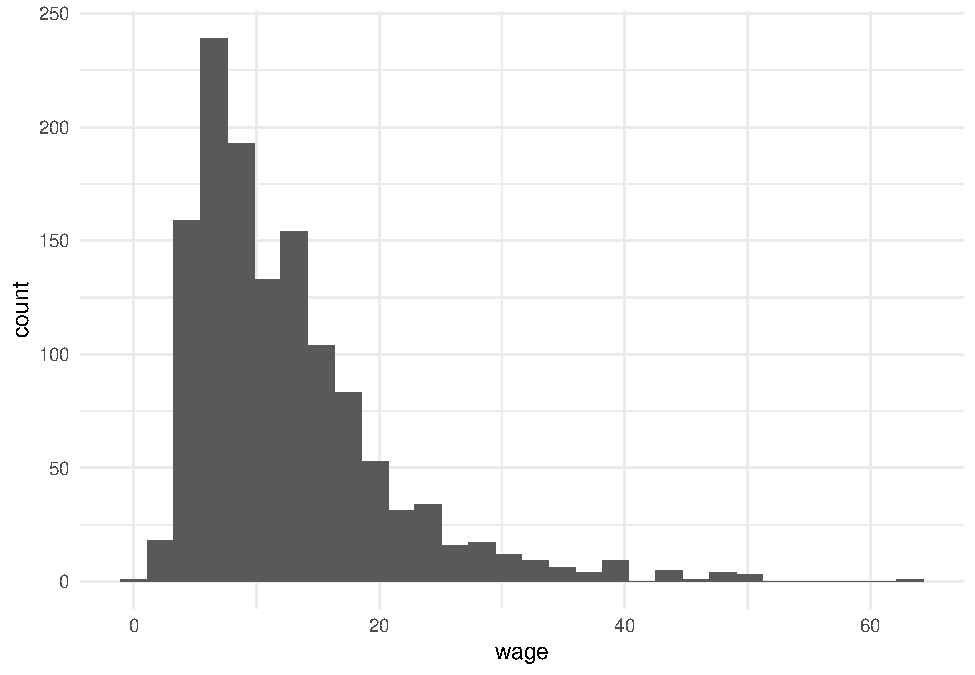
\includegraphics{rEkonometri_files/figure-latex/unnamed-chunk-219-1.pdf}

wage denilen saatlik ücretin sağa doğru uzanan bir kuyruğu olduğunu görüyoruz. Yani, veriler sağa çarpıktır. Buna bakmanın diğer iki yolu aşağıdaki gibidir.

Kümülatif dağılım:

\begin{Shaded}
\begin{Highlighting}[]
\KeywordTok{ggplot}\NormalTok{(df, }\KeywordTok{aes}\NormalTok{(}\DataTypeTok{x =}\NormalTok{ wage)) }\OperatorTok{+}
\StringTok{  }\KeywordTok{stat_ecdf}\NormalTok{(}\DataTypeTok{geom =} \StringTok{"step"}\NormalTok{, }\DataTypeTok{pad =} \OtherTok{FALSE}\NormalTok{) }\OperatorTok{+}
\StringTok{  }\KeywordTok{theme_minimal}\NormalTok{()}
\end{Highlighting}
\end{Shaded}

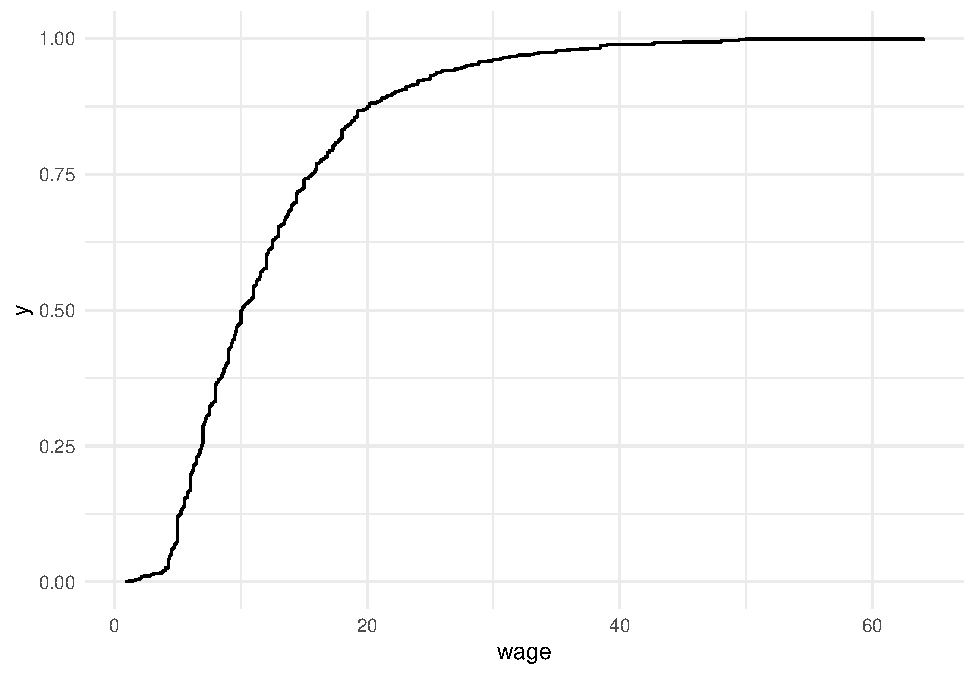
\includegraphics{rEkonometri_files/figure-latex/unnamed-chunk-220-1.pdf}

Kümülatif dağılım fonksiyonun tersi dilimlerdir (\(Q_p = F^{-1}\)).

\begin{Shaded}
\begin{Highlighting}[]
\KeywordTok{ggplot}\NormalTok{(df, }\KeywordTok{aes}\NormalTok{(}\DataTypeTok{x =}\NormalTok{ wage)) }\OperatorTok{+}
\StringTok{  }\KeywordTok{stat_ecdf}\NormalTok{(}\DataTypeTok{geom =} \StringTok{"step"}\NormalTok{, }\DataTypeTok{pad =} \OtherTok{FALSE}\NormalTok{) }\OperatorTok{+}
\StringTok{  }\KeywordTok{theme_minimal}\NormalTok{() }\OperatorTok{+}
\StringTok{  }\KeywordTok{coord_flip}\NormalTok{()}
\end{Highlighting}
\end{Shaded}

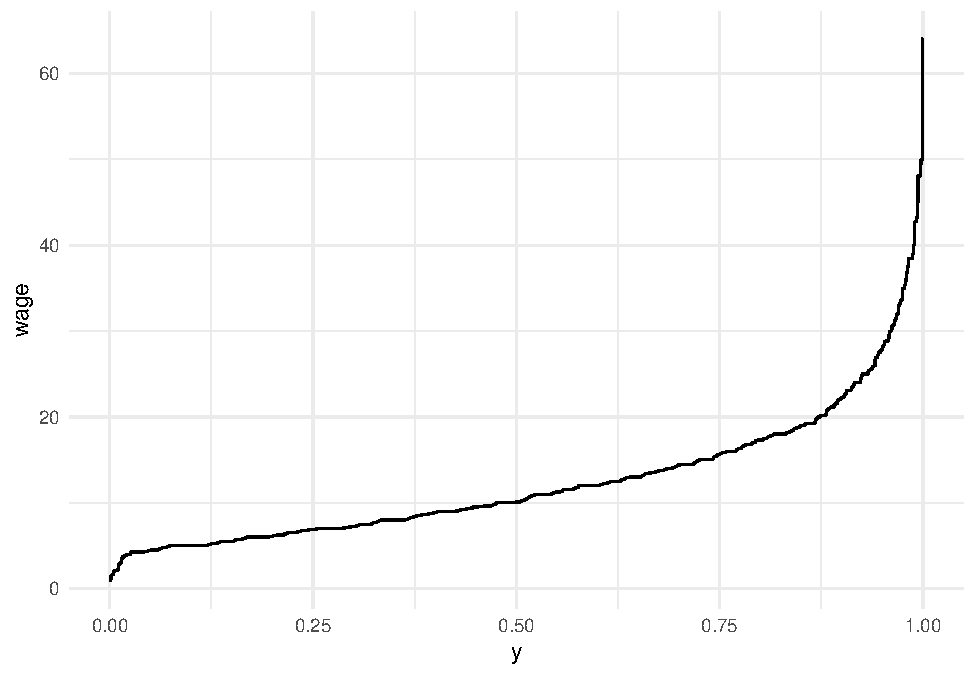
\includegraphics{rEkonometri_files/figure-latex/unnamed-chunk-221-1.pdf}

Modeli kurabiliriz. İlk olarak 50. yüzdelik dilimin (medyan) sonuçlarına bakalım.

\begin{Shaded}
\begin{Highlighting}[]
\NormalTok{model50 <-}\StringTok{ }\KeywordTok{rq}\NormalTok{(}\DataTypeTok{formula =}\NormalTok{ wage }\OperatorTok{~}\NormalTok{., }\DataTypeTok{tau =} \FloatTok{0.5}\NormalTok{, }\DataTypeTok{data =}\NormalTok{ df)}
\KeywordTok{summary.rq}\NormalTok{(model50)}
\end{Highlighting}
\end{Shaded}

\begin{verbatim}
## 
## Call: rq(formula = wage ~ ., tau = 0.5, data = df)
## 
## tau: [1] 0.5
## 
## Coefficients:
##             Value    Std. Error t value  Pr(>|t|)
## (Intercept) -5.92744  0.70550   -8.40174  0.00000
## female      -2.78430  0.31616   -8.80670  0.00000
## nonwhite    -0.82269  0.38292   -2.14848  0.03186
## union        1.67795  0.40668    4.12594  0.00004
## education    1.17843  0.04617   25.52450  0.00000
## exper        0.15224  0.01418   10.73325  0.00000
\end{verbatim}

education'daki 1 birimlik değişim ortalama saatlik ücrette 1.37 \$'lık (bir önceki çıktıya bakın) artışa neden olmaktadır şeklinde yorumluyorduk. Bunu artık 1 birimlik bir değişime karşın medyan ücret oranındaki değişim olarak yorumlayacağız.

exper 1 yıl arttığında medyan ücret 0.15 \$ artar (bir önceki çıktıyla neredeyse aynı).

Kadınların medyan ücreti erkeklerden 2.78 \$ daha düşüktür (female).

Sendikalı işçilerin medyan ücreti sendikalı olmayan işçilerden 1.68 \$ daha yüksektir (union).

Beyaz olmayanların medyan ücreti beyaz işçilerden 0.82 \$ daha düşüktür (nonwhite).

Karşılaştırma yapmak amacıyla 25. ve 75. dilimleri de ekleyelim. regresyon istenilen bir dilimde kurulabilir.

\begin{Shaded}
\begin{Highlighting}[]
\NormalTok{model25 <-}\StringTok{ }\KeywordTok{rq}\NormalTok{(}\DataTypeTok{formula =}\NormalTok{ wage }\OperatorTok{~}\NormalTok{., }\DataTypeTok{tau =} \FloatTok{0.25}\NormalTok{, }\DataTypeTok{data =}\NormalTok{ df)}
\KeywordTok{summary.rq}\NormalTok{(model25)}
\end{Highlighting}
\end{Shaded}

\begin{verbatim}
## 
## Call: rq(formula = wage ~ ., tau = 0.25, data = df)
## 
## tau: [1] 0.25
## 
## Coefficients:
##             Value    Std. Error t value  Pr(>|t|)
## (Intercept) -2.10096  0.71646   -2.93244  0.00342
## female      -2.04231  0.25255   -8.08660  0.00000
## nonwhite    -0.94423  0.19874   -4.75113  0.00000
## union        2.45385  0.27365    8.96705  0.00000
## education    0.70385  0.05933   11.86407  0.00000
## exper        0.09904  0.01109    8.93143  0.00000
\end{verbatim}

\begin{Shaded}
\begin{Highlighting}[]
\NormalTok{model75 <-}\StringTok{ }\KeywordTok{rq}\NormalTok{(}\DataTypeTok{formula =}\NormalTok{ wage }\OperatorTok{~}\NormalTok{., }\DataTypeTok{tau =} \FloatTok{0.75}\NormalTok{, }\DataTypeTok{data =}\NormalTok{ df)}
\KeywordTok{summary.rq}\NormalTok{(model75)}
\end{Highlighting}
\end{Shaded}

\begin{verbatim}
## 
## Call: rq(formula = wage ~ ., tau = 0.75, data = df)
## 
## tau: [1] 0.75
## 
## Coefficients:
##             Value    Std. Error t value  Pr(>|t|)
## (Intercept) -8.17417  1.12813   -7.24574  0.00000
## female      -3.70917  0.46120   -8.04239  0.00000
## nonwhite    -1.50667  0.45322   -3.32439  0.00091
## union        0.68000  0.60359    1.12659  0.26013
## education    1.55250  0.07796   19.91333  0.00000
## exper        0.25333  0.02158   11.73927  0.00000
\end{verbatim}

Dilim parametreleri kendi aralarında istatistiksel olarak farklılaşır mı? Aşağıdaki test ile parametre değerlerinin dilimler arasında aynı olduğu hipotezini güçlü bir şekilde reddediyoruz.

\begin{Shaded}
\begin{Highlighting}[]
\KeywordTok{anova.rq}\NormalTok{(model25, model50, model75)}
\end{Highlighting}
\end{Shaded}

\begin{verbatim}
## Quantile Regression Analysis of Deviance Table
## 
## Model: wage ~ female + nonwhite + union + education + exper
## Joint Test of Equality of Slopes: tau in {  0.25 0.5 0.75  }
## 
##   Df Resid Df F value    Pr(>F)    
## 1 10     3857  17.846 < 2.2e-16 ***
## ---
## Signif. codes:  0 '***' 0.001 '**' 0.01 '*' 0.05 '.' 0.1 ' ' 1
\end{verbatim}

\hypertarget{yararlanux131lan-kaynaklar}{%
\chapter{Yararlanılan Kaynaklar}\label{yararlanux131lan-kaynaklar}}

\emph{Temel Ekonometri; Damodar N. Gujarati, Dawn C. Porter (Ümit Şenesen, Gülay Günlük Şenesen)}

\emph{Örneklerle Ekonometri; Damodar Gujarati (Nasip Bolatoğlu)}

\emph{Örneklerle Ekonometri Veri Setleri: \url{https://www.macmillanihe.com/companion/gujarati-econometrics-by-example-2e/learning-resources/Data-sets/}}

\emph{Ekonometriye Giriş; James H. Stock, Mark W. Watson (Bedriye Saraçoğlu)}

\emph{Ekonometri Kılavuzu; Peter Kennedy (Şenay Açıkgöz, Muzaffer Sarımeşeli)}

\emph{Ekonometrik Çözümleme; William H. Greene (Ümit Şenesen)}

\emph{Ekonometriye Giriş Modern Yaklaşım; Jeffrey M. Wooldridge (Ebru Çağlayan)}

\emph{Ekonometri Temel Kavramlar; Ebru Çağlayan, Selahattin Güriş}

\href{https://www.sas.upenn.edu/~fdiebold/Teaching221/FullBook.pdf}{\emph{Elements of Forecasting; Diebold}}

\href{https://www.tcmb.gov.tr/wps/wcm/connect/TR/TCMB+TR/Main+Menu/Yayinlar/Raporlar/Enflasyon+Raporu/2020/Enflasyon+Raporu+2020+-+I}{\emph{Enflasyon Raporu 2020 - I (30 Ocak 2020)}}

\href{http://professor.ufabc.edu.br/~nelson.faustino/Ensino/IPE2016/Livros/Peter\%20L.\%20Bernstein-Against\%20the\%20Gods_\%20The\%20Remarkable\%20Story\%20of\%20Risk-Wiley\%20(1998)\%20(1).pdf}{\emph{Tanrılara Karşı Riskin Olağanüstü Tarihi; Peter L. Bernstein (Canan Feyyat)}}

\href{https://www.bbc.com/news/magazine-13775520}{\emph{Francis Galton: The man who drew up the `ugly map' of Britain}}

\href{http://galton.org/books/finger-prints/galton-1892-fingerprints-1up.pdf}{\emph{Finger Prints}}

\href{https://www.toraks.org.tr/uploadFiles/book/file/1832014154715-113.pdf}{\emph{İstatistik Sonuçlarının Yorumu: p Değeri ve Güven Aralığı Nedir?}}

\href{https://www.tepav.org.tr/upload/mce/2019/haberler/gece_isiklariyla_il_bazinda_gsyh_tahmini_19922018.pdf}{\emph{1992-2018 Dönemi için Gece Işıklarıyla İl Bazında GSYH Tahmini: 2018'de 81 İlin Büyüme Performansı}}

\href{https://nptel.ac.in/content/storage2/courses/105108079/module7/lecture31.pdf}{\emph{Stochastic Hydrology}}

\href{http://www.acarindex.com/dosyalar/makale/acarindex-1423937309.pdf}{\emph{Çoklu Doğrusal Bağlantı Halinde En Küçük Kareler Tekniğinin Alternatifi Yanlı Tahmin Teknikleri ve Bir Uygulama}}

\href{http://static.dergipark.org.tr:8080/article-download/imported/1025008693/1025007279.pdf?}{\emph{Çoklu Doğrusal Bağlantı Durumunda Ridge ve Temel Bileşenler Regresyon Analiz Yöntemlerinin Kullanımı}}

\href{https://dspace.ankara.edu.tr/xmlui/bitstream/handle/20.500.12575/59591/20427.pdf?sequence=1\&isAllowed=y}{\emph{Yumurta tavukçuluğunda gelirin Ridge Regresyon analizi ile tahmini}}

\href{https://www2.stat.duke.edu/courses/Spring19/sta101.002/post/project/outliers.html}{\emph{Outliers, Leverage Points and Influential Points}}

\href{https://www.researchgate.net/profile/Gozde_Koca/publication/324831528_EKONOMETRIDE_GUNCEL_KONULAR/links/5c2c88c992851c22a3547b3f/EKONOMETRIDE-GUeNCEL-KONULAR.pdf\#page=32}{\emph{Ekonometride Güncel Konular: Mixed Logit Modeli}}

\href{https://www.gecekitapligi.com/Webkontrol/uploads/Fck/yayin4_3.pdf\#page=88}{\emph{Van Belediyelerinin Hizmetlerine Yönelik Memnuniyetin Genelleştirilmiş Sıralı Logit Modeli ile Analizi}}

\href{https://www.semanticscholar.org/paper/Lung-Cancer-Study-with-Tobit-Regression-Analysis\%3A-Zorlutuna-Erilli/327a4952217d1c03c603db02fa6c43c47873f2c0}{\emph{Lung Cancer Study with Tobit Regression Analysis: Sivas Case}}

\href{http://auzefkitap.istanbul.edu.tr/kitap/iktisat_ue/uygulamaliista.pdf}{\emph{Uygulamalı İstatistik}}

  \bibliography{book.bib}

\end{document}
